% !TEX root = ./../main.tex
\chapter{Results}
\label{chap:results}
The results summarized in section~\ref{sec:NPMembraneInt} were obtained using the \ac{STD} \martini{} \ac{FF}, 
with a cut--off method for treating the electrostatic interactions. Unfortunately, as we have seen in 
chapter~\ref{chap:EmpiricalFF}, such method poorly describes the processes that involve the transfer of a charged 
moiety from a polar (e.g. water) environment to an non--polar one (e.g. the membrane core).

Our aim is thus to perform a comparison between the \ac{STD} \martini{} model and two versions of \martini{} that 
better take into account electrostatic interactions. We will consider
\begin{enumerate}[label=\itshape\roman*.]
	\item the \martini{} \ac{FF} with long range electrostatics (\martini{} + \ac{PME});
	\item the \martini{} \ac{FF} with long range electrostatics and \ac{PW} (\martini{} + \ac{PME}/\acs{PW}).
\end{enumerate}

In this chapter we present the main results of this thesis. In section~\ref{sec:resultsBiased} we calculate, using 
the metadynamics method, the free energy barrier for the \ac{NP} anchoring (and dis--anchoring) process using 
versions \textit{i}. and \textit{ii}. of the \martini{} \ac{FF}, and compare the outcomes to those obtained with 
the \ac{STD} \martini{} model and with atomistic simulations. The introduction of long--range electrostatics has 
the overall effect of increasing the energy barriers for the translocation of charged ligands.

In section~\ref{sec:resultsUnBiased} we focus on the description of the molecular processes that take place during the anchoring/dis--anchoring of the \ac{NP}. This analysis will be applied to both biased (metadynamics) trajectories and unbiased \ac{MD} runs, and it will allow to quantify the degree of alteration of the membrane structural properties during the interaction with the \ac{NP}.

% The pathway to improve the model is the use of the \ac{PME} method to better describe the electrostatic interaction and the use of the \ac{PW} model to improve the behavior of the water solvent at a \ac{CG} level. For a comparison to be made, the idea, is to follow the procedure describe in section~\ref{sec:preliminaryMetadyn} and, with metadynamics runs, try to estimate the energy barrier of the anchoring process with the use of the \ac{PME} alone and in combination with the \ac{PW} model.
%
% Preliminary, some tests about the use of the \ac{PME} method and the \ac{PW} model with a pure \ac{POPC} bilayer was performed. Then metadynamics runs for obtaining the \ac{FES} of the anchoring process involving both the striped (\ac{MUS}:\ac{OT} $1$:$1$) and the random (\ac{MUS}:\ac{OT} $1$:$1$) \acp{NP} were performed with the use of the \ac{PME} alone and in combination with the \ac{PW}.
%In view of the results, then, as better described in the next chapter, unbiased \ac{MD} runs with the use of \ac{PME} and \ac{PW} involving all the \ac{NP} configurations were performed in order to investigate a possible change in the kinematic of the all the \ac{NP}--membrane interaction process.

\section{Thermodynamic results}
\label{sec:resultsBiased}
The process that I will consider for the \ac{FES} estimation of the ligand anchoring is composed of two steps: the 
forward process: from the hydrophobic state to the state with one anchor; the backward process: from the anchored 
state to the hydrophobic state again.

\paragraph{\textbf{system set--up}} In all of my biased and unbiased \ac{MD} runs the membrane bilayer is made of 
$256$ \ac{POPC} lipids per leaflet. I will consider both the striped (\ac{MUS}:\ac{OT} $1$:$1$) and the random 
(\ac{MUS}:\ac{OT} $1$:$1$) \acp{NP}. The simulation box is neutralized with $30$ counteracting Na$^+$ 
ions\footnote{The \martini{} model for ions, especially for Na$^+$ and Cl$^-$, associates the ion plus the 
hydration shell to a bead of type Qd positively charged and Qa negatively charged, respectively.} and filled by 
water. In figure~(\ref{fig:startFrameHydro}) it is shown an example of the starting configuration for a striped 
(\ac{MUS}:\ac{OT} $1$:$1$) \ac{NP} in the hydrophobic state. The initial configuration frames with the \ac{PW} are 
obtained from the initial configuration frames with the \ac{STD} \martini{} water using a python script that 
converts the \ac{STD} \martini{} water to the \ac{PW} bead. With the \ac{PW} an equilibration run with the 
parameters shown in the third column of table~(\ref{tab:inputParam}) is necessary to stabilize the system. As 
already shown in figure~(\ref{fig:CVRappresentation}), our metadynamics runs use as \ac{CV} the distance between 
one single charged ligand terminal and the \ac{COM} of \ac{POPC} along the normal. The charged ligand for the 
anchoring process is chosen so as to be the lowest charged ligand attached to the \ac{NP} core. For what concerns 
the metadynamics input parameters used to perform my \ac{MD} runs, if not differently specified, they are 
summarized in table~(\ref{tab:metadynParam}).
\begin{SCfigure}[][!ht]
	\centering
	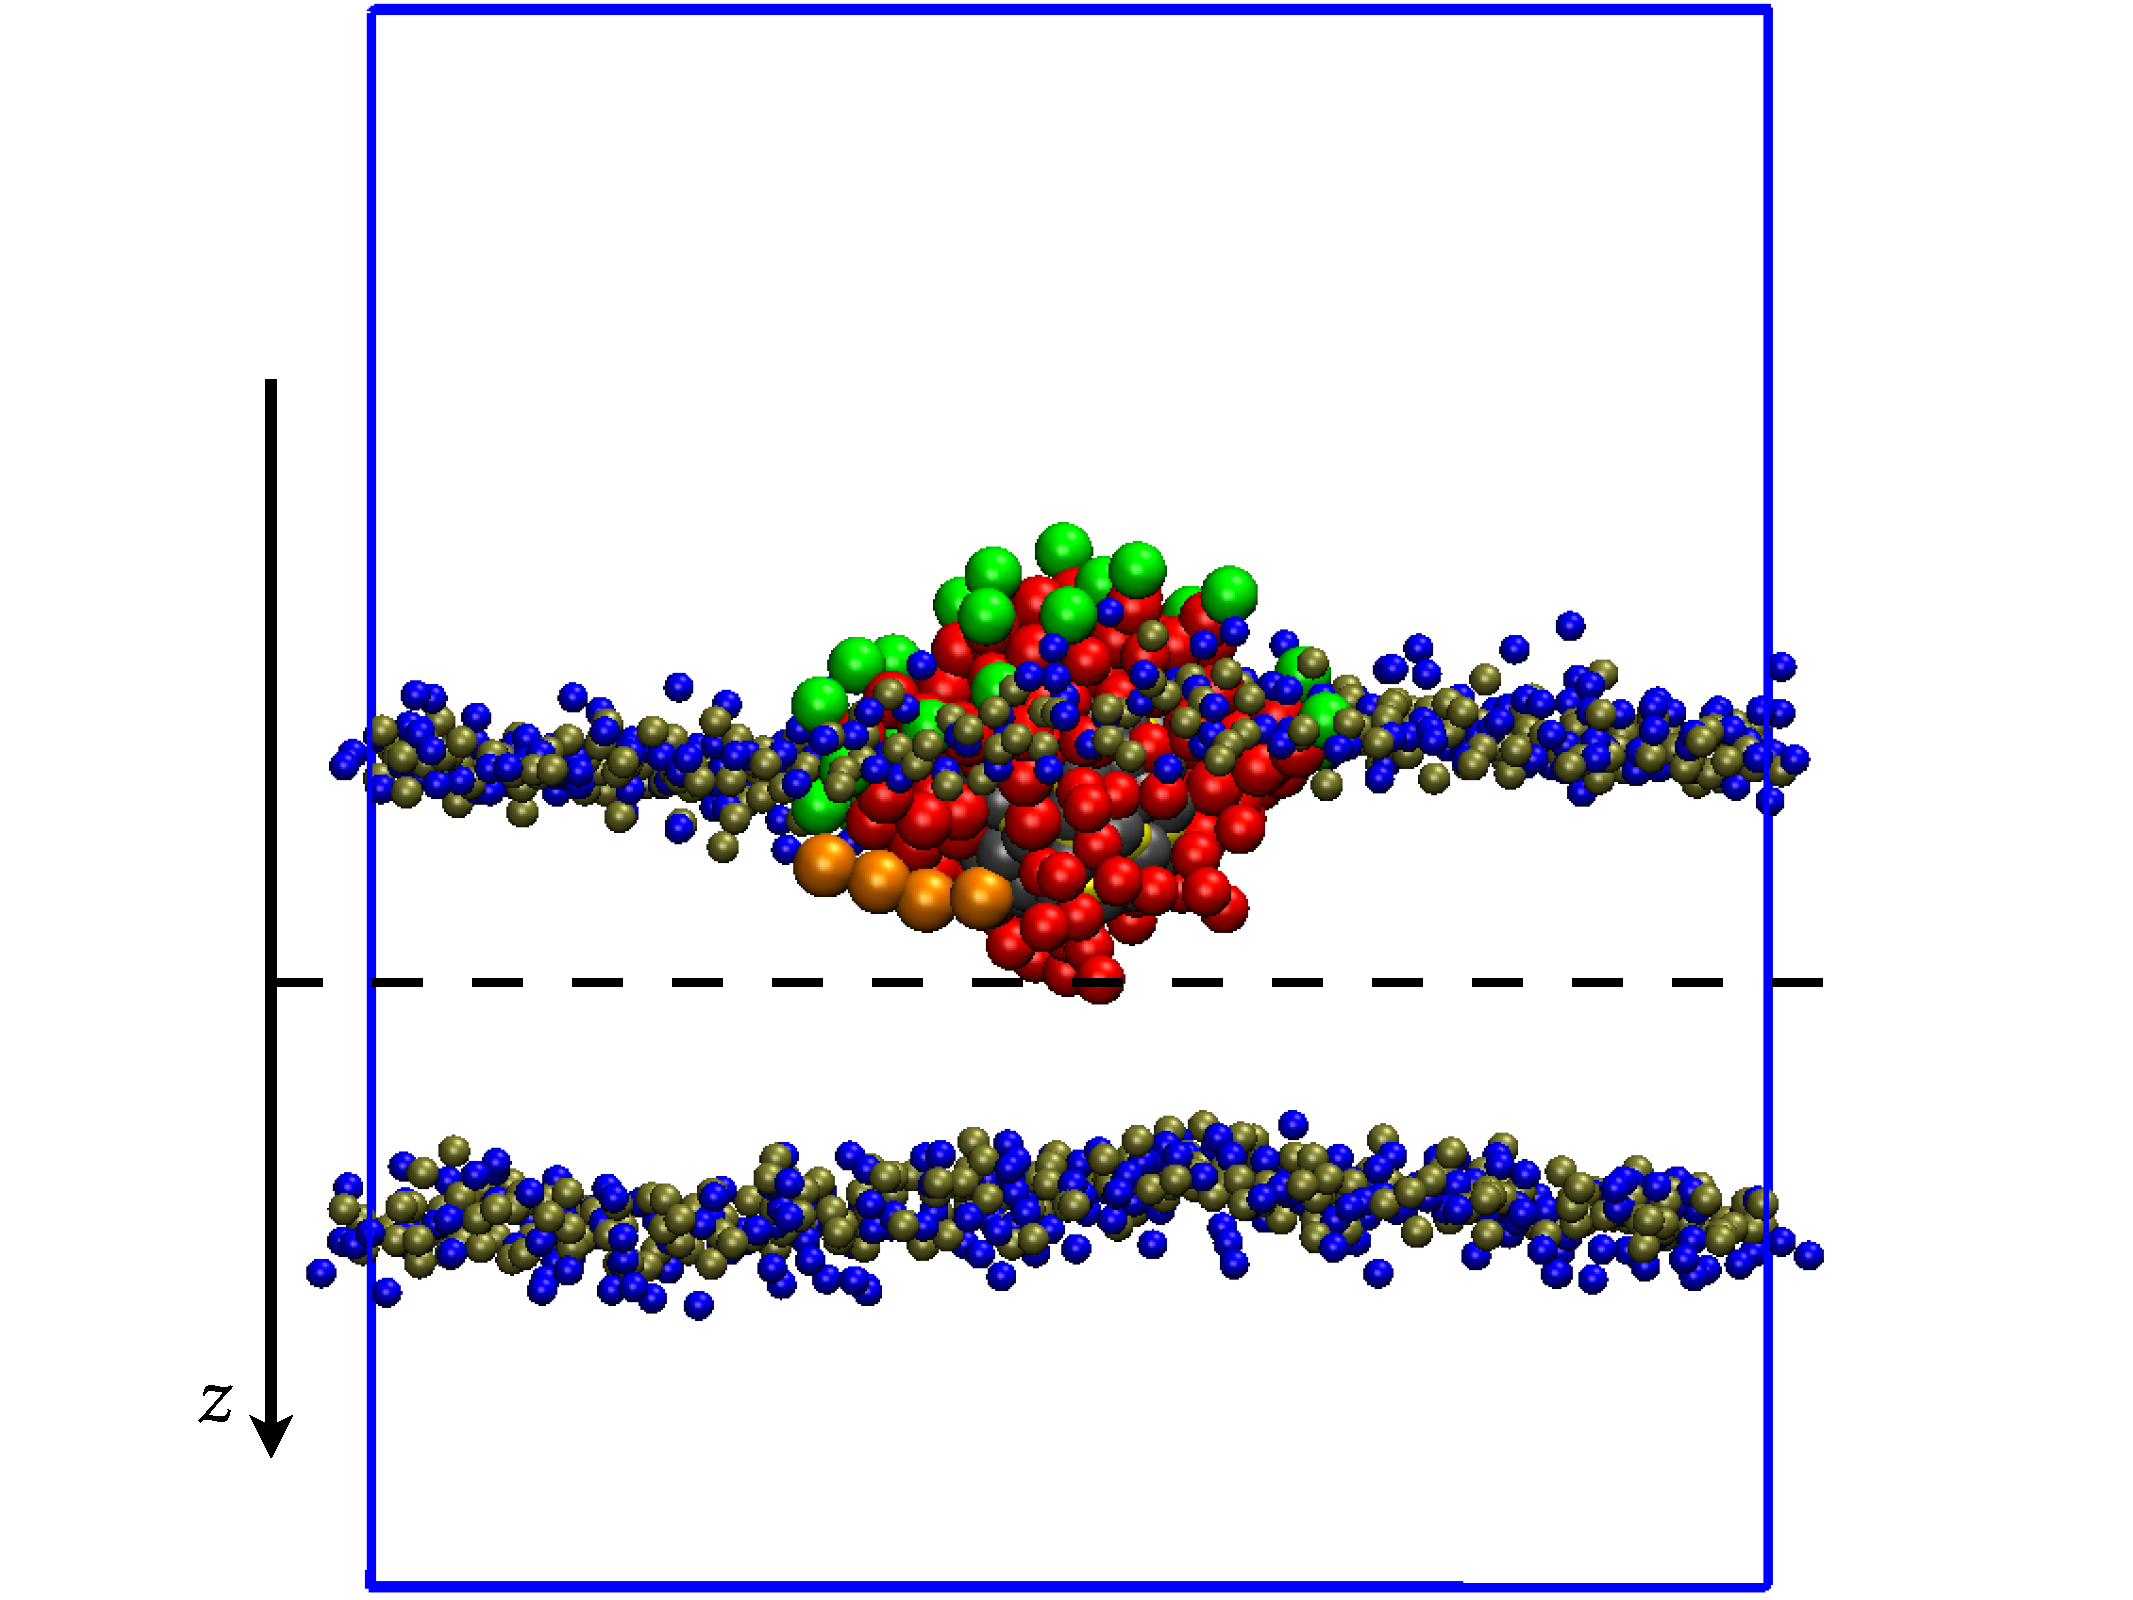
\includegraphics[width=0.42\textwidth]{./img/patchedHydrophobic.pdf}
	\caption{Example of a starting configuration of a metadynamics run of a striped (\ac{MUS}:\ac{OT} $1$:$1$) \ac{NP} in the hydrophobic state. Color code as in figure~(\ref{fig:threeProcess}). The charged ligand chosen for the anchoring process is in orange. The dashed line is the center of the bilayer. The blue contour is the simulation box. Water beads and lipid tails are not shown.}%
	\label{fig:startFrameHydro}
\end{SCfigure}

% \paragraph{\textbf{CV issues}} The \ac{CV} chosen to describe the anchoring process is the $z$ component of the distance between the center of the charged bead and the \ac{COM} of the bilayer. Although this \ac{CV} is a very intuitive and simple, with the introduction of the \ac{PME} method, and more accentuated with the \ac{PW} model, we found that it suffers of some issues. When I perform the metadynamics runs with the \ac{PME} and \ac{PW}, in accordance with the atomistic results, it is observed that the anchored state is more stable than with the \ac{STD} \martini{} models: the increase of the model accuracy make the interaction between the negatively charged bead and the positively charged choline group of the lipid heads of the opposite leaflet, stronger than with the \ac{STD} \martini{}. The same apply with the \ac{PW} beads. Hence, like in figure~(\ref{fig:engulfment}), we observe that when the metadynamics try to dis--anchor the charged bead in the backward process, it pull back the lipid heads slightly deforming the opposite leaflet of the bilayer. This results in a worse estimation of the \ac{CV} because the charged ligand is in the hydrophobic region near the entrance leaflet but still in contact with one or two lipid heads of the opposite leaflet.
% \begin{SCfigure}[][h!t]
% 	\centering
% 	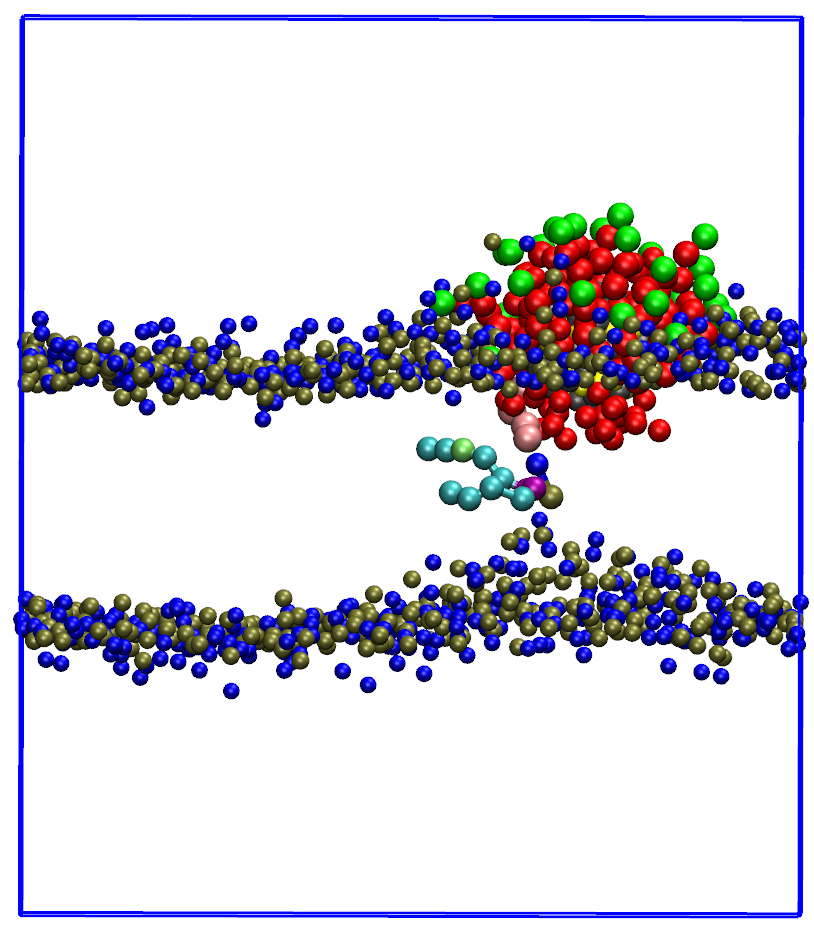
\includegraphics[width=0.5\textwidth]{./img/patchedEngulfment}
% 	\caption{Detail of the engulfment effect in the anchoring leaflet when the ligand tends to dis--anchor. Color code as in figure~(\ref{fig:threeProcess}). Lipid tails are shown in cyan while the glycerol group is represented by the violet beads. Water and other lipid tails are not shown. The choline group (blue bead) is in contact with the charged bead of the ligand (pink beads) and the lipid tails are horizontal instead of vertical as they usually are.}
% 	\label{fig:engulfment}
% \end{SCfigure}
% Another import issue as the simulation time increase and related to the previous issues, is the loss of the ability by the \ac{CV} to well distinguish the two states, although the convergence has not yet reached. In figure~(\ref{fig:NPDist}) the red line is the \ac{CV}. In the region $z > 1$ the ligand have crossed the \ac{COM} of the bilayer and it is anchored in the opposite leaflet. For $z < -1$ the ligand is near the \ac{NP}'s leaflet in the hydrophobic state. While for $-1 < z < 1$ the ligand is in the hydrophobic region of the membrane but it may be in contact with the lipid head beads of the opposite leaflet. Hence inside the dashed black lines there is a region of the \ac{CV} space in which the two states are overlapping. This issue leads in a underestimation of the forward wall of the one anchor \ac{FES} because it tend to lower the saddle point while the metadynamics is still sampling the anchored state.
% \begin{figure}[!ht]
% 	\centering
% 	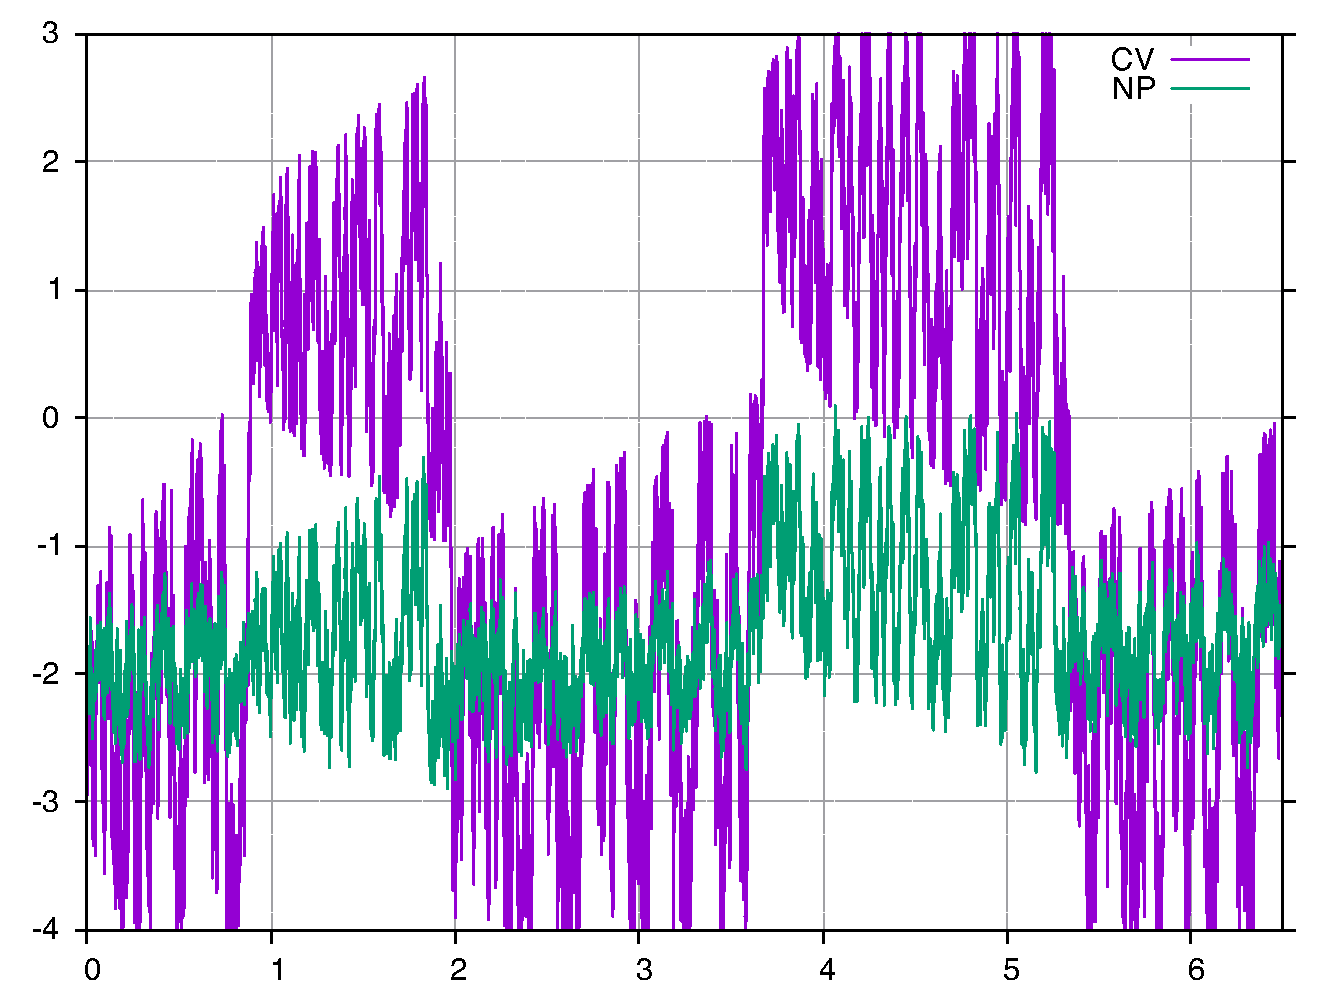
\includegraphics[width=0.7\textwidth]{./img/results/NPDistance/NPDist}
% 	\caption{Correlation between the \acs{CV} (red) and the $z$ component of the distance between the \acs{COM} of the \acs{NP} and the \acs{COM} of the bilayer (green) as a function of the simulation time. The region of the \acs{CV} space inside the dashed black lines is the overlapping region. Data obtained from a $6.5$~$\mu$s metadynamics run of a striped (\acs{MUS}:\acs{OT} $1$:$1$) \acs{NP} with \acs{PW}.}
% 	\label{fig:NPDist}
% \end{figure}
%
% %Moreover, since the interaction with the lipid heads is stronger,
%
% \paragraph{\textbf{convergence problems}} An important issue related to this process is the achievement of the convergence, essential in the \ac{FES} estimation. Our metadynamics runs have not reached the convergence, even in tens of microseconds of simulation, as we can see from figure~(\ref{fig:NPDist}) (red) of a $6.5$~$\mu$s test run in which we try to reach the convergence\footnote{In this run in an attempt to speed up the achievement of the convergence, in addition to the metadynamics bias, I use two other harmonic bias to limit the sampled region. Un upper bias which is activated when the charged bead is far from the bilayer \acs{COM} for more than $3$~nm and a lower bias when the charged bead is far from the bilayer \acs{COM} for more than $-4$~nm. The elastic constant is chosen $k = 100$~kJ/mol for both.}. This is prevalently due to the just described issues associated to the \ac{CV}. But also, in accordance with my unbiased simulations and the atomistic results, because the energy barriers associated to the two metastable state are much higher than what are estimated in \cite{ourPaper}, slowing down the reaching of the convergence. Another issues is related to stronger interaction between the charged bead and the \ac{PW} beads and the charged bead and the lipid heads. From the metadynamics runs, for the random and more pronounced for the striped \acp{NP}, we observe that, respect to the \ac{STD} \martini{} model, the charged ligand spend a not negligible time completely soaked in the water phase ($z>-2$). This leads to sample a region of the \ac{CV} space useless for one anchor \ac{FES} estimation and tend to slow down the achievement of the convergence. Another undesired process that we observe as the simulation time increase, is a small drag of the \ac{NP} inside the bilayer by the charged ligand in the anchored state. From figure~(\ref{fig:NPDist}), since the stronger interaction with water, we see that when the charged bead is approaching the water phase of the opposite leaflet ($z>2$) it is not only due to the ligand itself but also because the \ac{COM} of the \ac{NP} tend to approach the \ac{COM} of the bilayer (green). Despite this can be an important molecular process in order for a comparison to be made, we must not sample the phase phase associated to the movement of the \ac{COM} of the \ac{NP} since we are interested in the \ac{FES} associated to the anchoring process only.
%
% \paragraph{\textbf{worse estimation of the FES}} From the previous explanations it is clear that following the procedure outlined in \cite{ourPaper} leads to a worse estimation of the \ac{FES} associated to the anchoring process. In particular all these issues suggest a different pathway, at molecular level, for the forward process respect to the backward process and that some other \acp{CV} are missing. Hence, using the same \ac{CV}, instead to try to estimate the whole \ac{FES}, we can try to estimate the energy wall associated to the forward process and, separately, the energy wall associated to the backward process. For the estimation of the energy wall of the forward process we need to start the metadynamics runs in the hydrophobic state and stop it when the ligand reach the anchored state. For the backward process we need to do the contrary: start the metadynamics from the anchored state and stop it when the ligand return to \ac{NP} leaflet. Then we can compare the new results with the \ac{STD} \martini{} model and the atomistic one.
%la usiamo per stimare la barriera di andata e ritorno

\subsection{Forward process}
I have performed ten metadynamics runs starting from the hydrophobic state for each of the following 
``configurations'': striped (\ac{MUS}:\ac{OT} $1$:$1$) with \ac{PME}; striped (\ac{MUS}:\ac{OT} $1$:$1$) with 
\ac{PME} and \ac{PW}; random (\ac{MUS}:\ac{OT} $1$:$1$) with \ac{PME} and \ac{PW}. In figure~(\ref{fig:metaFrame}) 
is shown a series of sequential frames of a metadynamics run of a striped \ac{NP} with \ac{PME}$+$\ac{PW} in which 
we can see the anchoring and dis--anchoring processes.
\begin{figure}[t!]
	\centering
		\subfloat[]{
		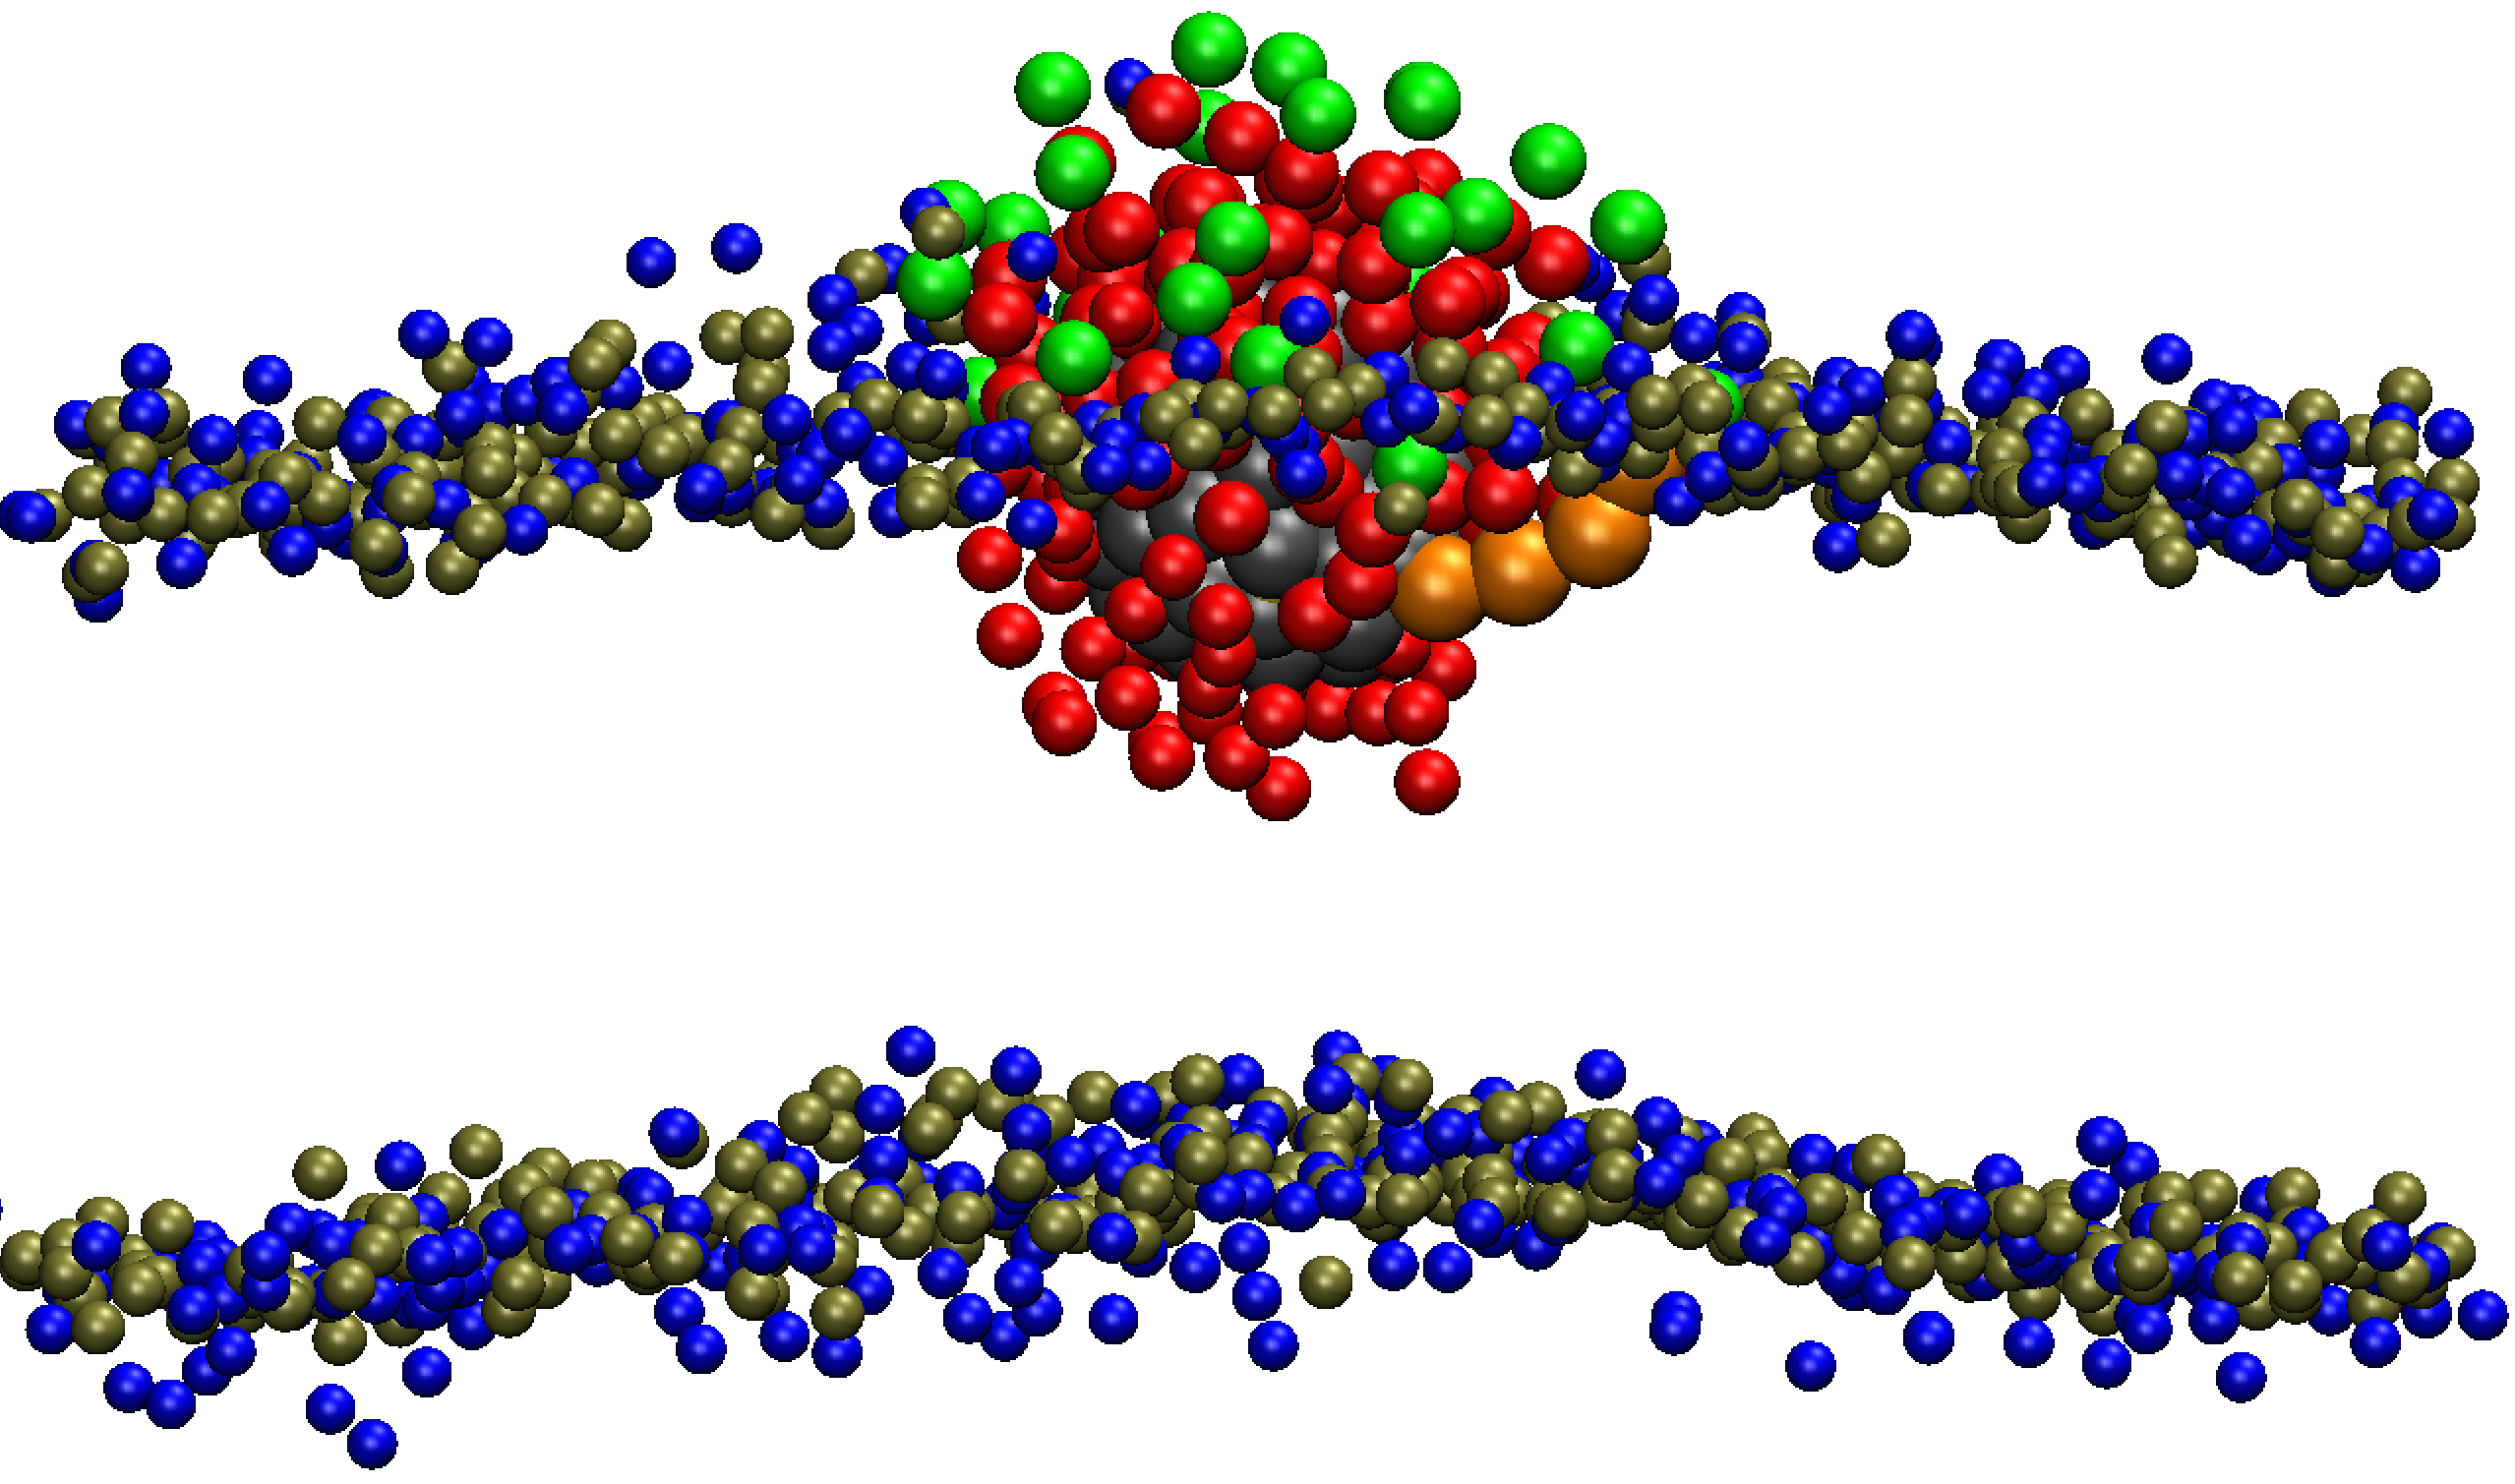
\includegraphics[width=0.47\textwidth]{./img/metadynFrame/a.png}
		}\ %
		\subfloat[]{
		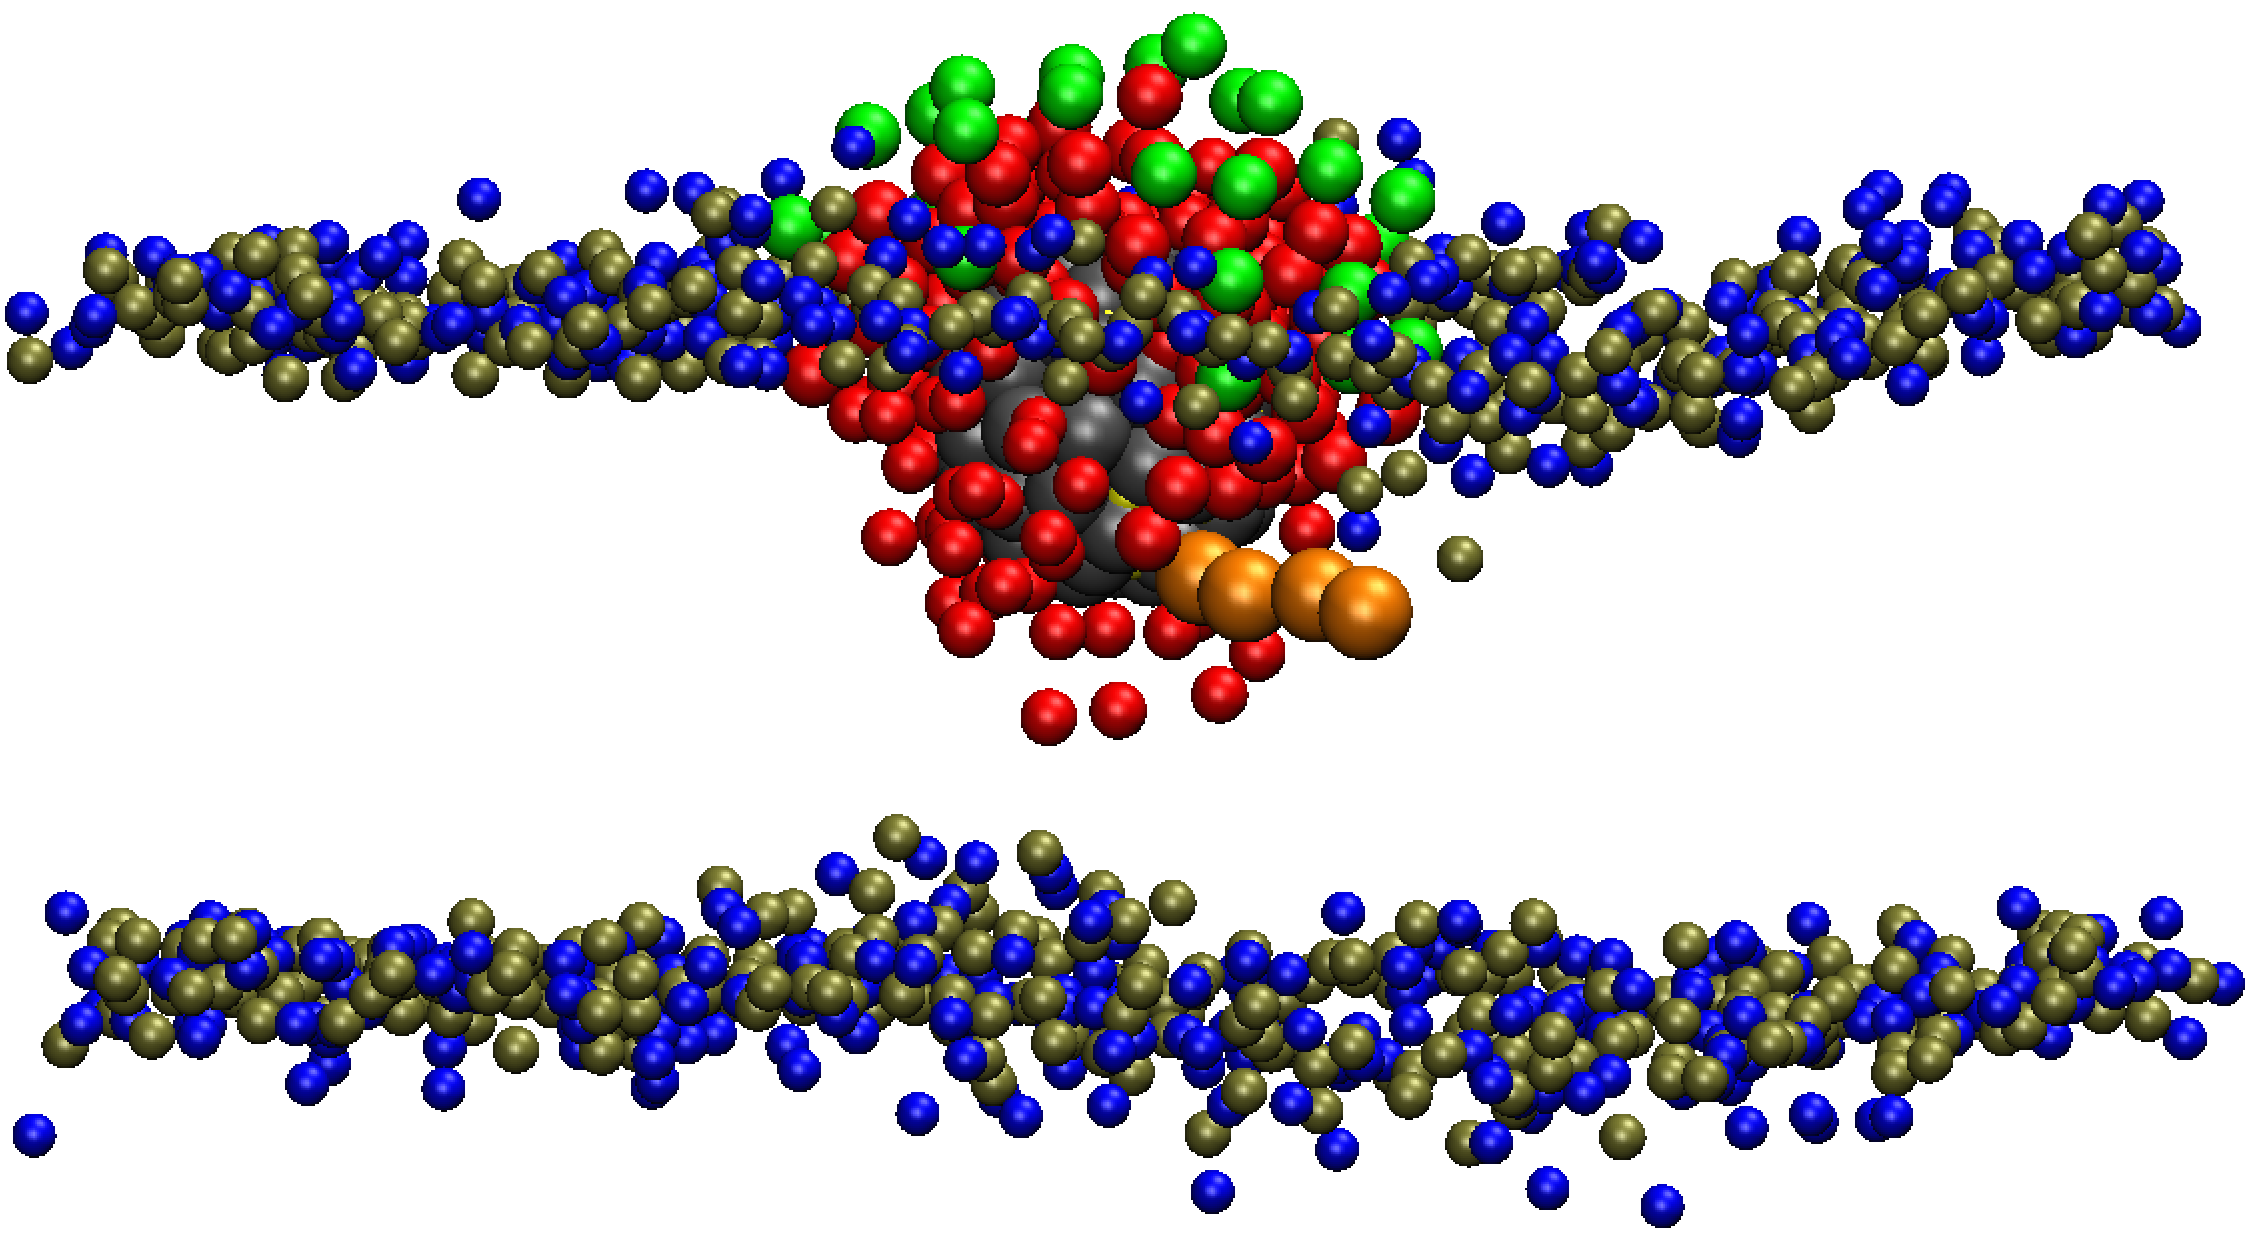
\includegraphics[width=0.47\textwidth]{./img/metadynFrame/b.png}
		}\\\medskip%
		\subfloat[]{
		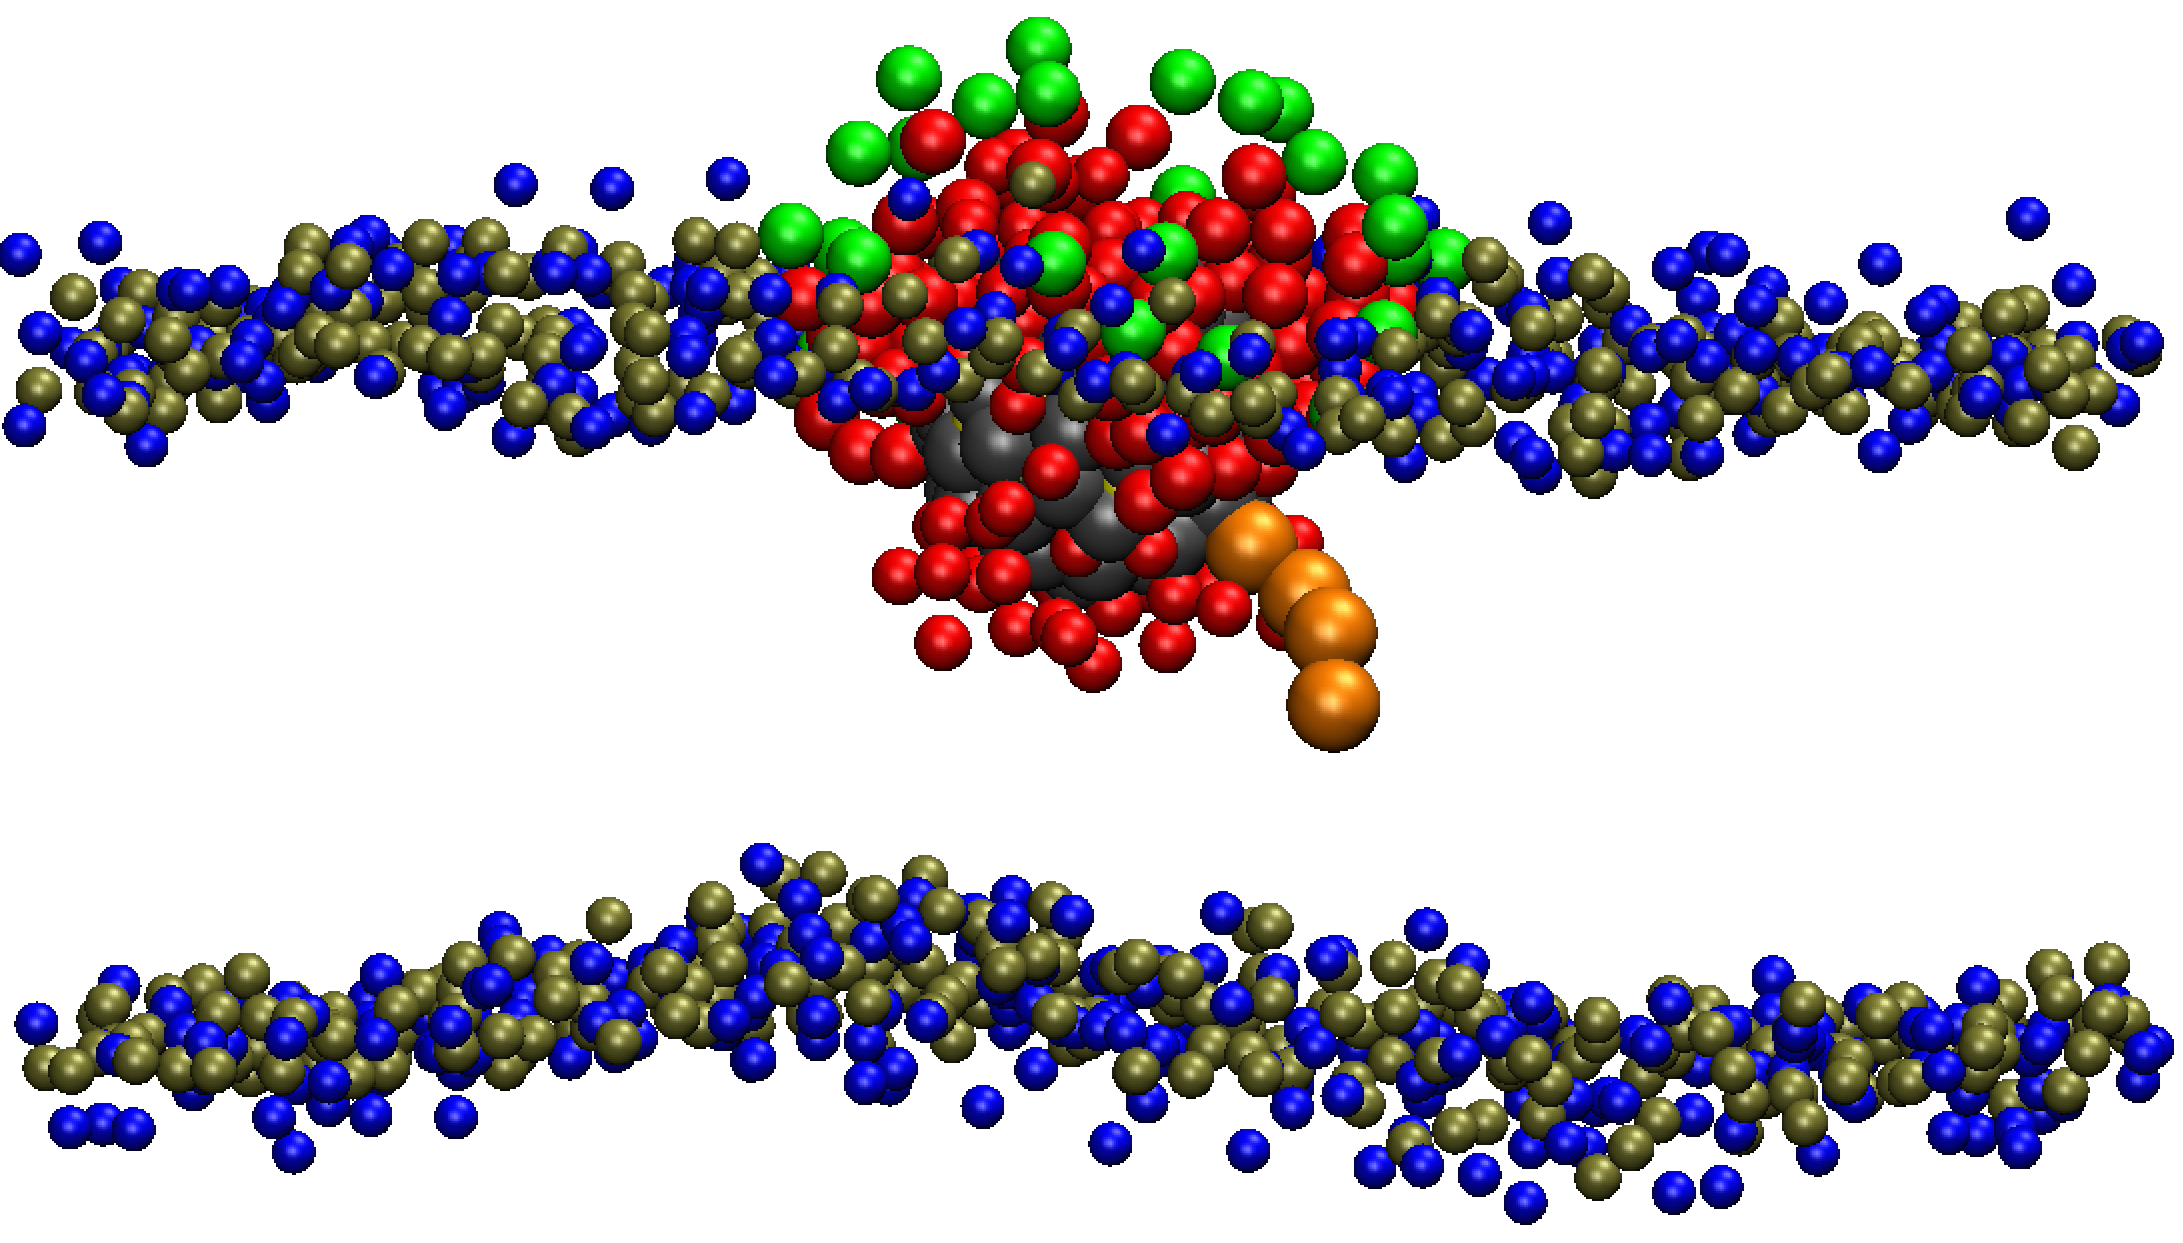
\includegraphics[width=0.47\textwidth]{./img/metadynFrame/c.png}
		}\ %
		\subfloat[]{
		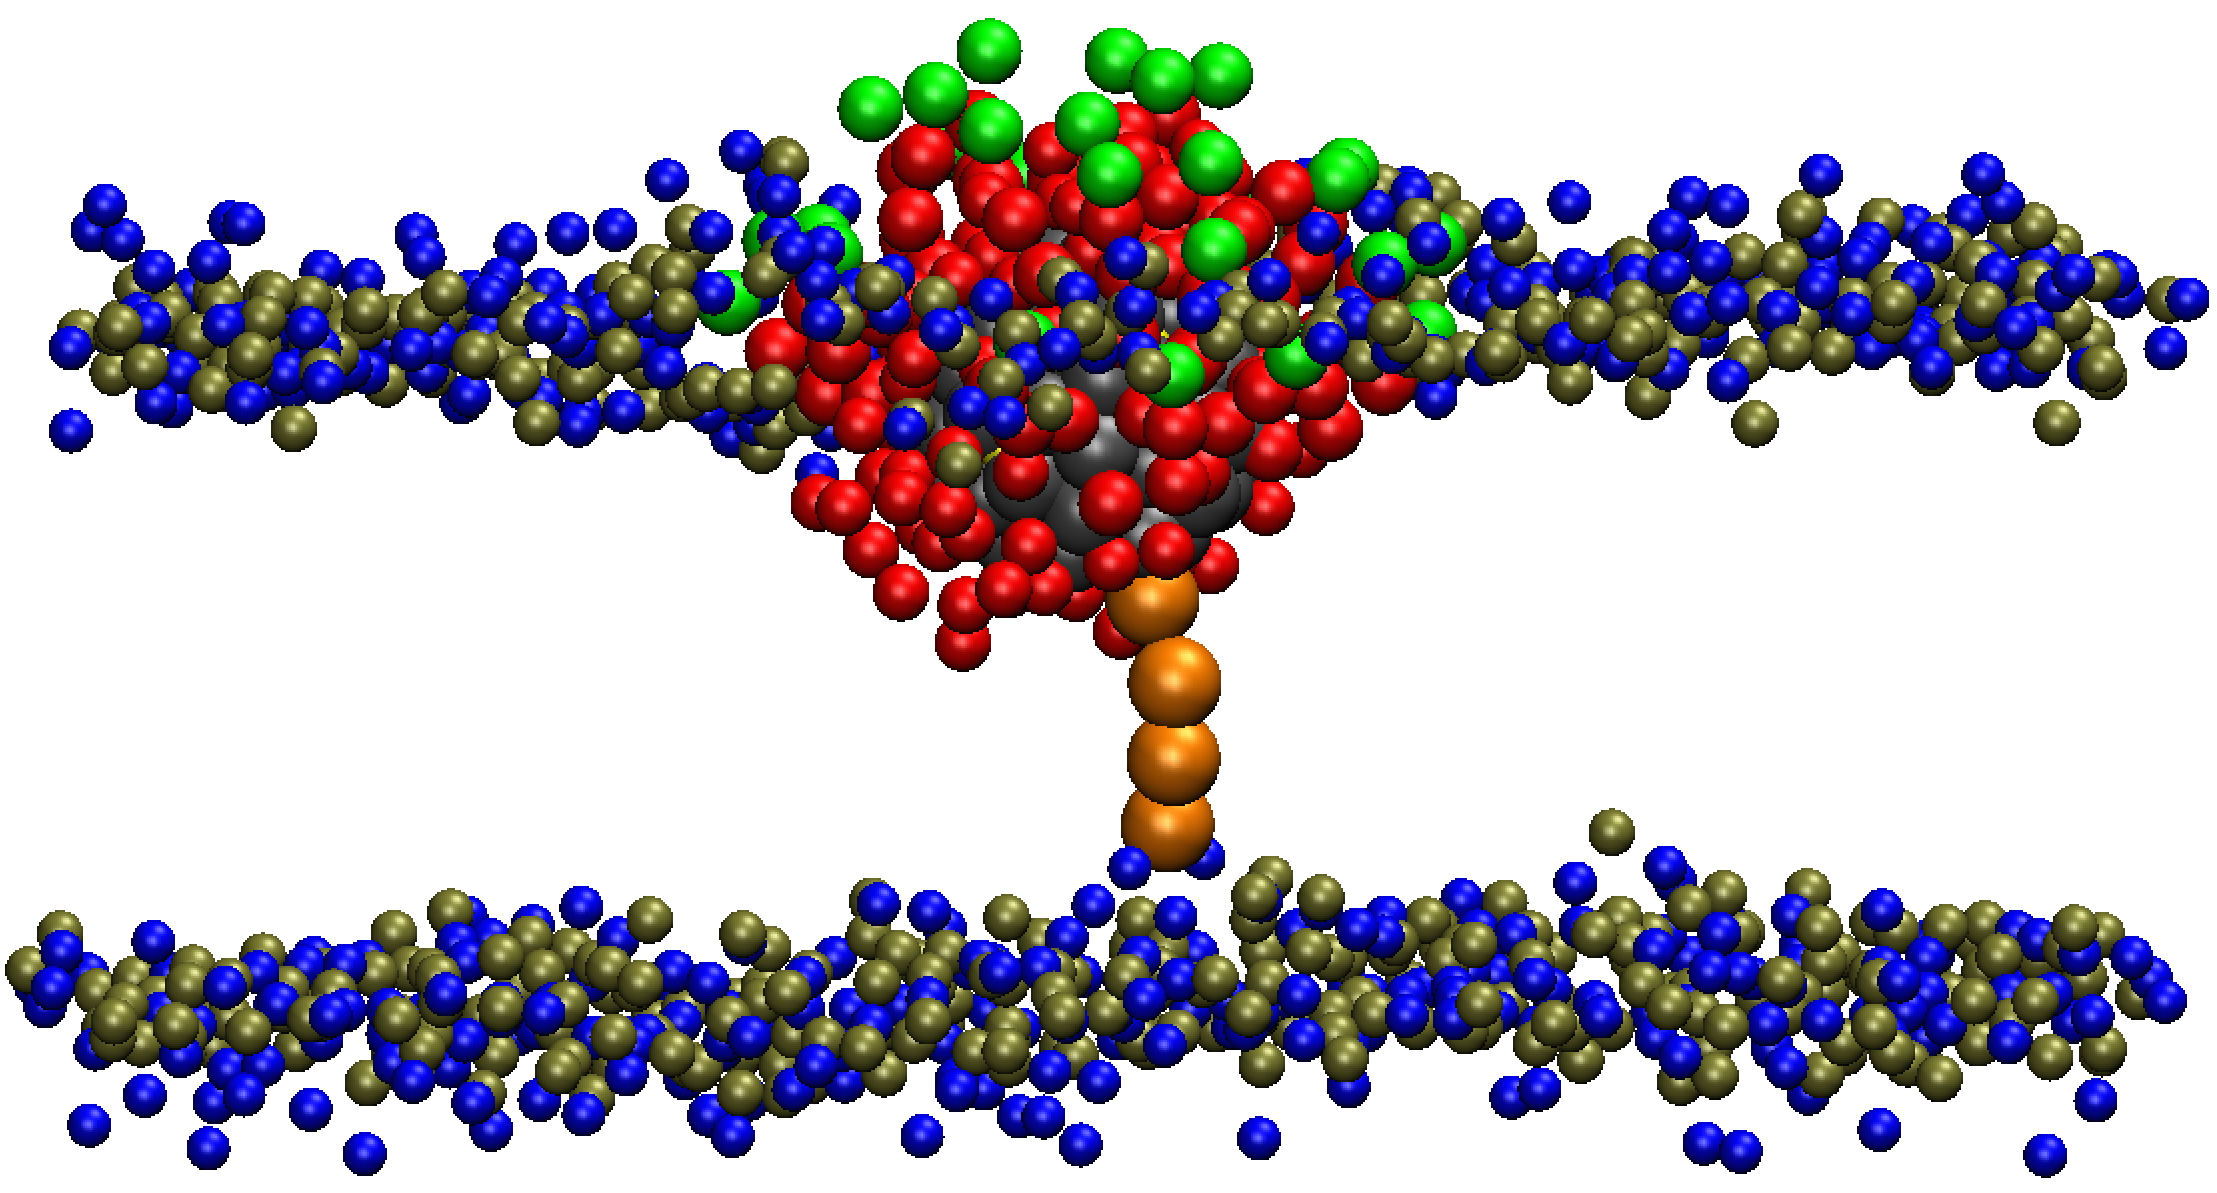
\includegraphics[width=0.47\textwidth]{./img/metadynFrame/d.png}
		}\\\medskip%
		\subfloat[]{
		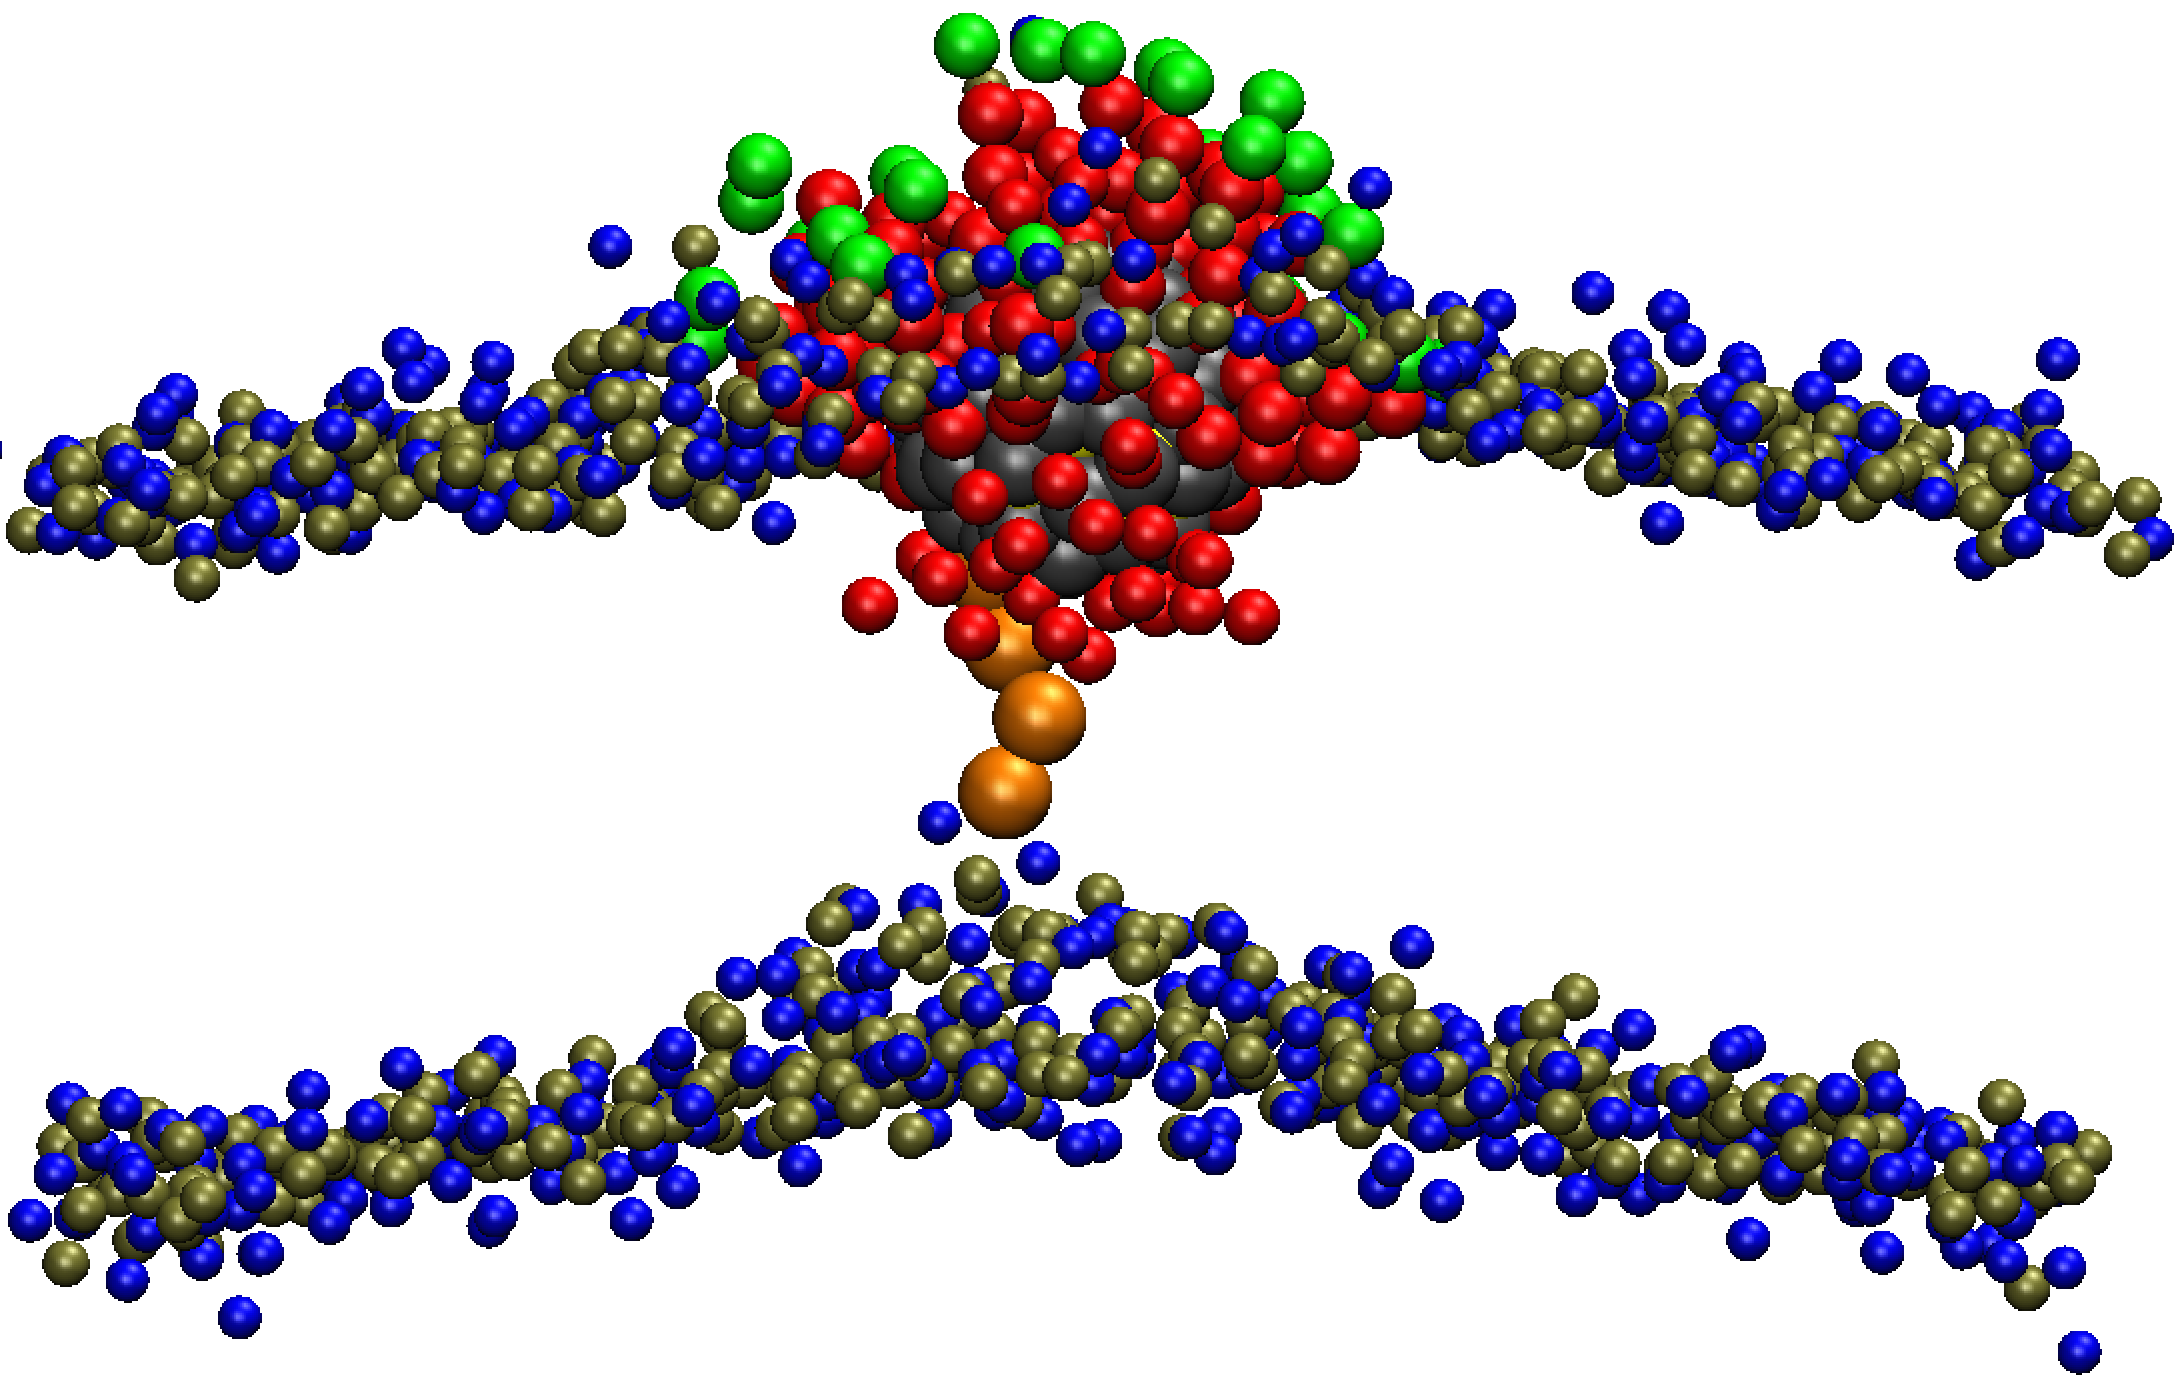
\includegraphics[width=0.47\textwidth]{./img/metadynFrame/e.png}
		}\ %
		\subfloat[]{
		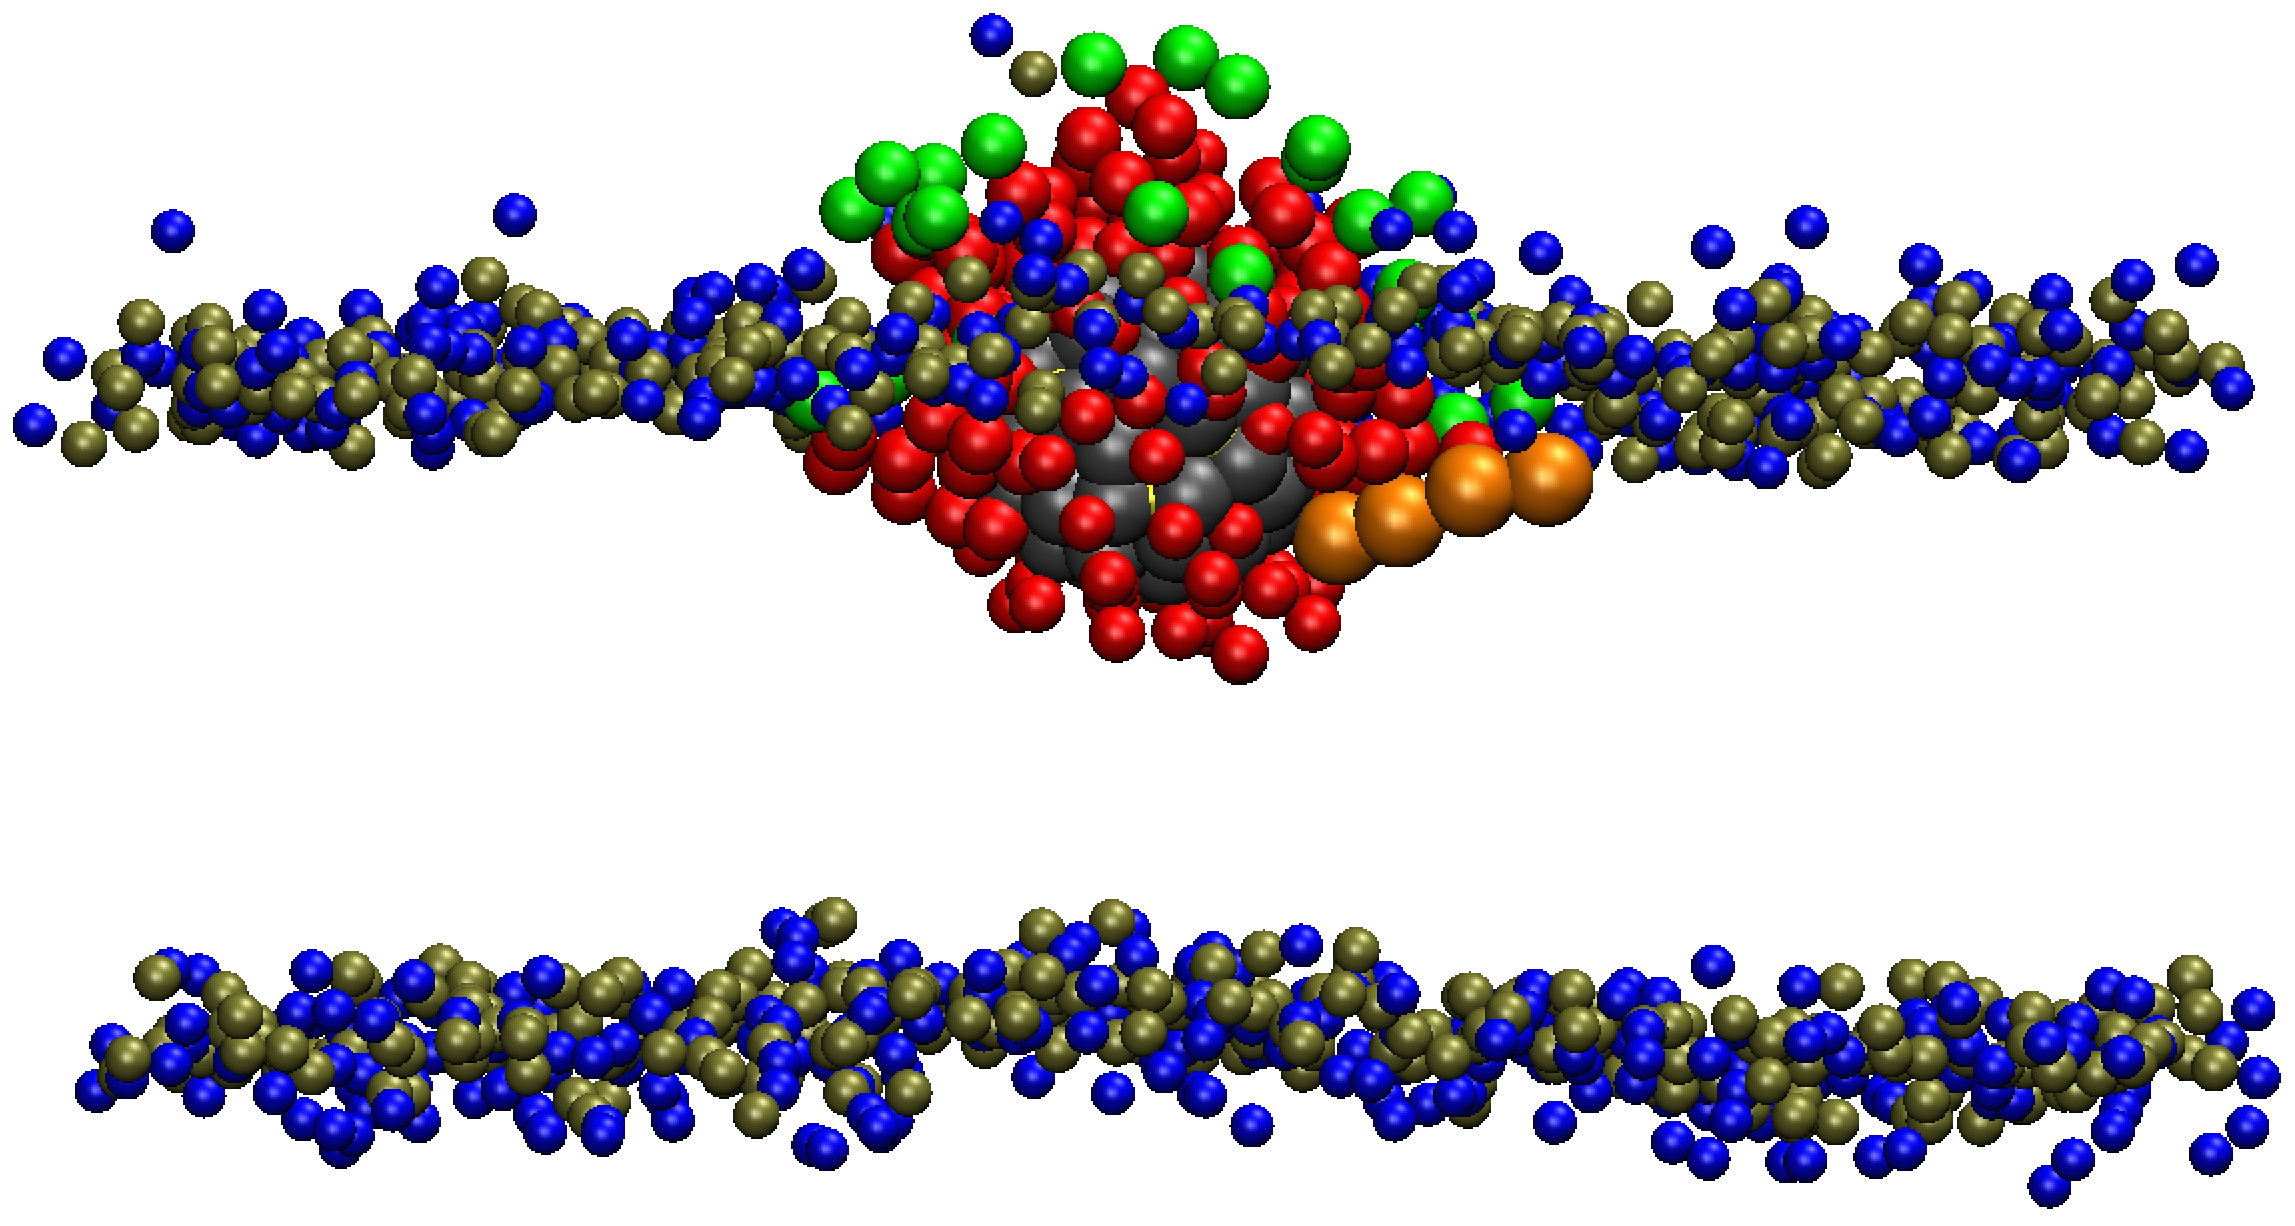
\includegraphics[width=0.47\textwidth]{./img/metadynFrame/f.png}
		}
	\caption{Series of sequential frames of a metadynamics run of a striped \ac{NP} with \acs{PME}$+$\acs{PW}. From (a) to (f): the starting frame in the hydrophobic contact, just before the anchoring, the charged ligand into the hydrophobic region of the bilayer, one anchor state, just before the dis--anchor and the final frame in the hydrophobic state again. Color code as in figure~(\ref{fig:threeProcess}). The charged ligand chosen for the metadynamics is in orange. Water and lipid tails are not shown.}%
	\label{fig:metaFrame}
\end{figure}

For a comparison between our \ac{CG} models and the atomistic model to be made all the distance variables 
involving the bilayer (e.g. the chosen \ac{CV}) are scaled by the ratio between the thickness of a pure \ac{POPC} 
bilayer as obtained with the atomistic \ac{FF} and the one obtained with the \ac{CG} \ac{FF}. This ratio is 
calculated from the bilayer's thickness shown in table~(\ref{tab:POPCData}).

A comparison of the forward barrier obtained for the striped (\ac{MUS}:\ac{OT} $1$:$1$) \ac{NP} with different 
models is shown in figure~(\ref{fig:forwardWall}a) and in table~(\ref{tab:hydroTime}) the average height of the 
barrier with the \ac{CG} models are summarized. The error is estimated using the standard error as in the 
procedure described in section~\ref{sec:metadynamics}. As we can see, increasing the accuracy of the \ac{CG} 
model, in particular with the use of the \ac{PW} model, the \ac{CG} results are approaching the atomistic one. The 
\ac{CG} and atomistic models differ also in terms of position of the minimum, which in the atomistic case is 
shifted by a few \r{A} towards the center of the membrane.

As we shall see later, the order of magnitude of the energy barrier is consistence with my unbiased simulations of 
all \acp{NP} with the \ac{PW} in which for ten of microseconds no anchor process is observed. This suggest that 
the energy wall is much higher than what is observed in \cite{ourPaper}. Another sign of the increasing of the 
energy wall as the \ac{CG} model accuracy increase, is the time spent by the \ac{NP} in the hydrophobic state. In 
table~(\ref{tab:hydroTime}) is shown a comparison of the average time spent by the \ac{NP} in the hydrophobic 
state between different \ac{CG} models.
\begin{table}[h!t]
	\centering\footnotesize
	\begin{tabular}{lccccc}
		\toprule
		\,	& striped($1$:$1$)	& striped($1$:$1$)	& striped($1$:$1$)	& random($1$:$1$)	& striped($1$:$1$) 	\\
		\,	& STD$^a$	& \acs{PME}$^b$	& \acs{PME}$+$\acs{PW}$^b$	& \acs{PME}$+$\acs{PW}$^b$ 	& atomistic$^c$		\\ \toprule
	$\overline{t_{h}}$ [ns]	& $\sim 140$& $\sim 215$	& $\sim 982$	& $\sim 413^d$ 	& $\sim 317$		\\ \midrule
	$\Delta G$ [kJ/mol] 	& $26 \pm 2$& $36 \pm 4$	& $100 \pm 5$	& $61 \pm 2$ 	& $134 \pm 5$		\\ \bottomrule
	\end{tabular}
	\caption{Summary of the metadynamics results on the striped and the random \acp{NP} for the forward process. $\overline{t_h}$ is the average time spent by the \acs{NP} in the hydrophobic state. $\Delta G$ is the average height of the forward energy barrier. The error is the standard error of the mean value. $^a$ Data obtained from \cite{ourPaper}. $^b$ Data obtained from my \acs{MD} runs. $^c$ Data courtesy of Federica Simonelli. $^d$ A comparison with the other values is no possible due to the different dynamics between a \ac{CG} and an atomistic model; moreover the metadynamics run for the atomistic model was made with Gaussians bigger than what are used for the \ac{CG} run, speeding up amazingly the forward process.}%
	\label{tab:hydroTime}
\end{table}

%Margins: in=3cm, out=4cm
\begin{figure}[pth]
	\centering
	\begin{adjustwidth}{-1.5cm}{-0.5cm}
		\subfloat[Striped NP: models comparison]{%
		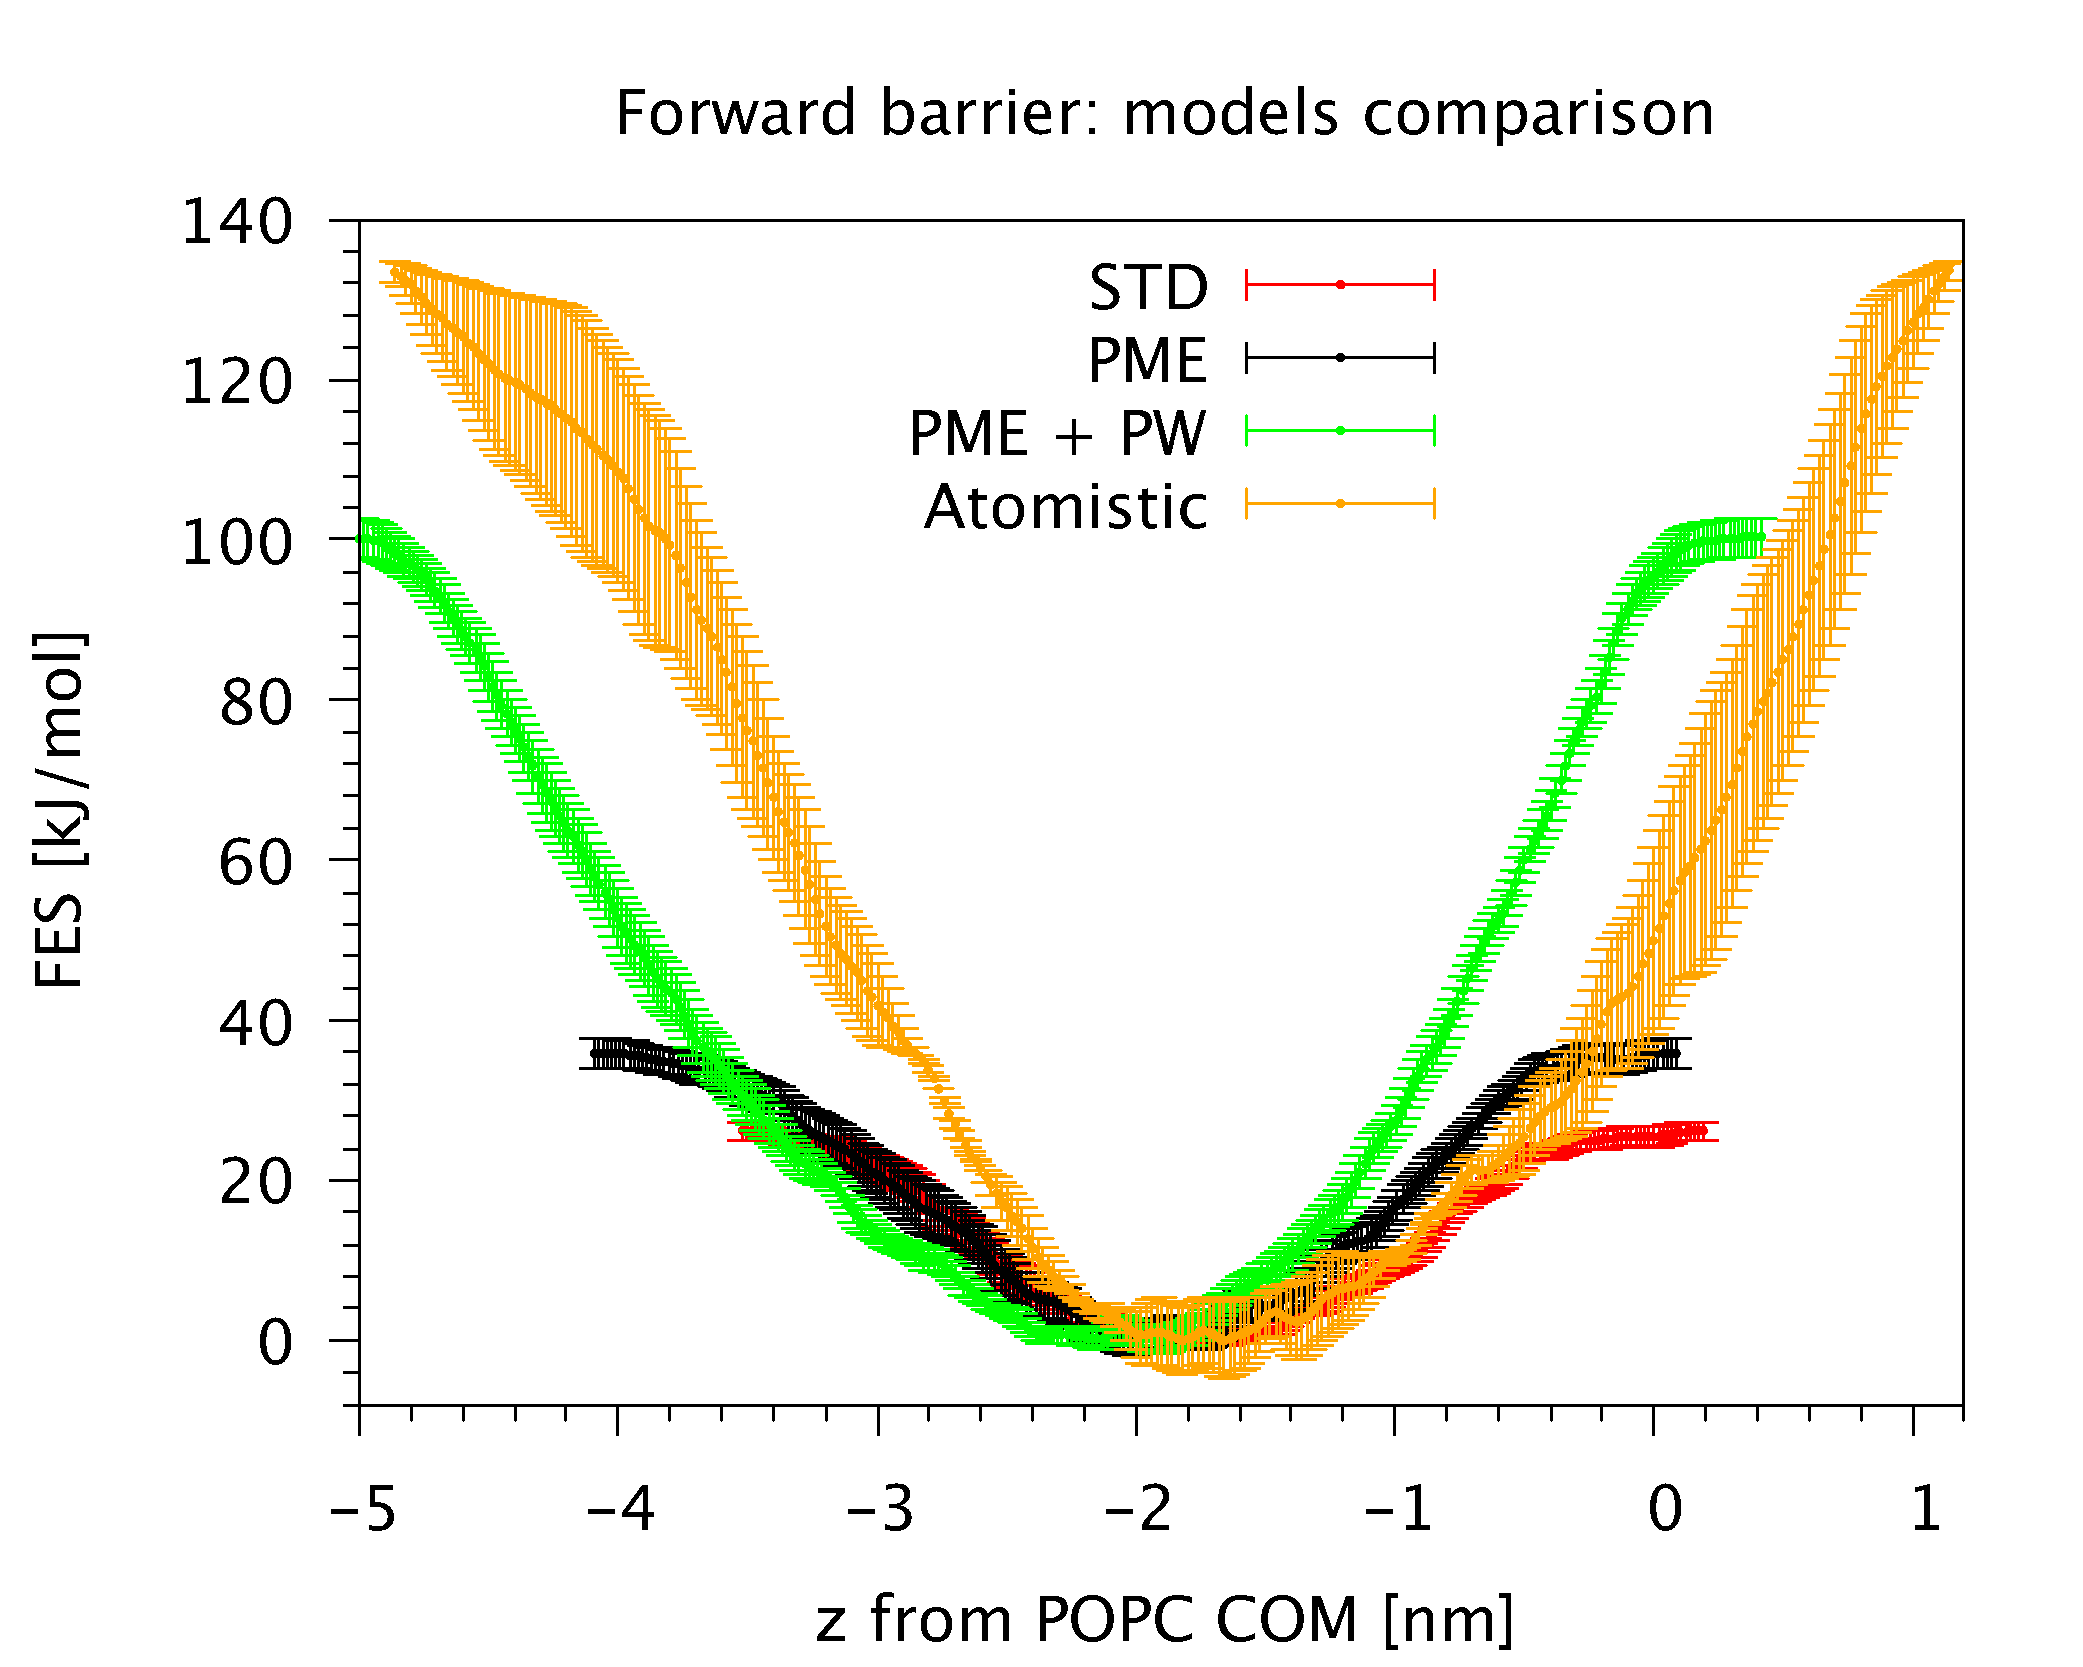
\includegraphics[width=0.5\linewidth]{./img/results/forwardWall}%
		}%
		\subfloat[Random and striped NP comparison]{%
		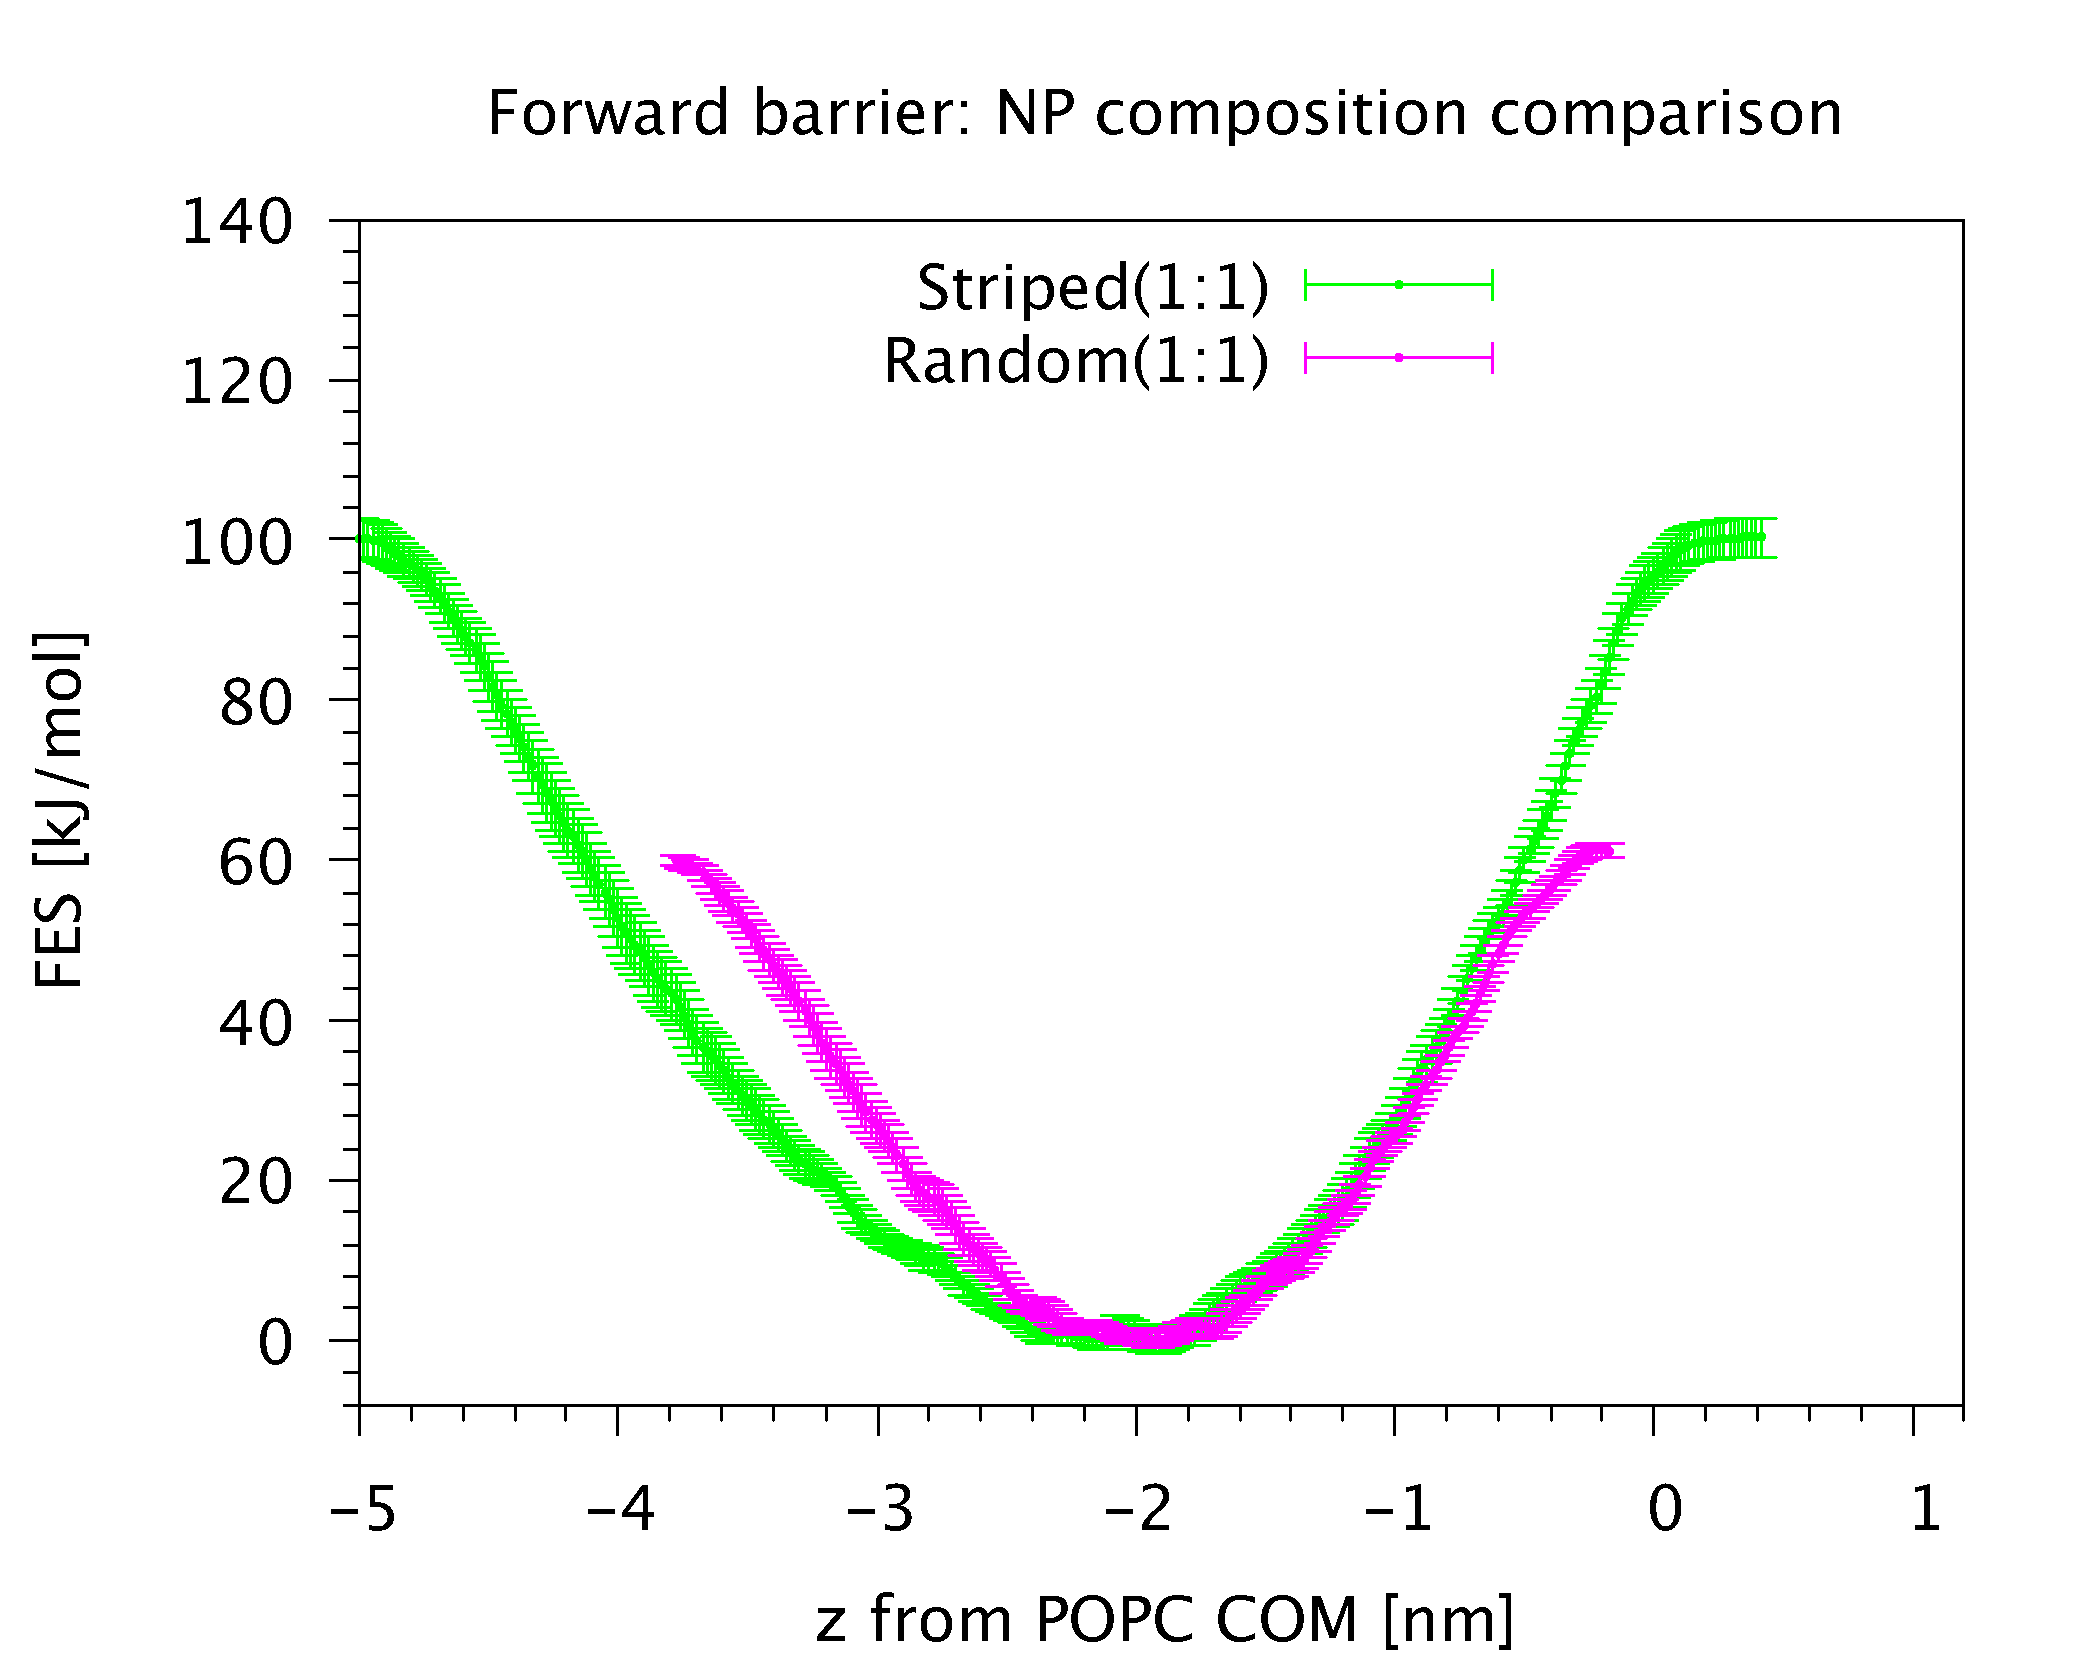
\includegraphics[width=0.5\linewidth]{./img/results/forwardWallRP}%
		}%
		\caption{\acs{FES} of the forward energy barrier as a function of the \acs{CV}. (a) In a comparison with different models. (b) In a comparison with the striped and the random \acp{NP} with \acs{PME} and \acs{PW}. The data for the STD version are an average over eight runs; for the \acs{PME} and \acs{PME}+\acs{PW} are an average over ten simulations each and the atomistic data are an average over two runs.}%
		\label{fig:forwardWall}%

		\vspace*{\floatsep}%

		\subfloat[Striped NP: models comparison]{%
		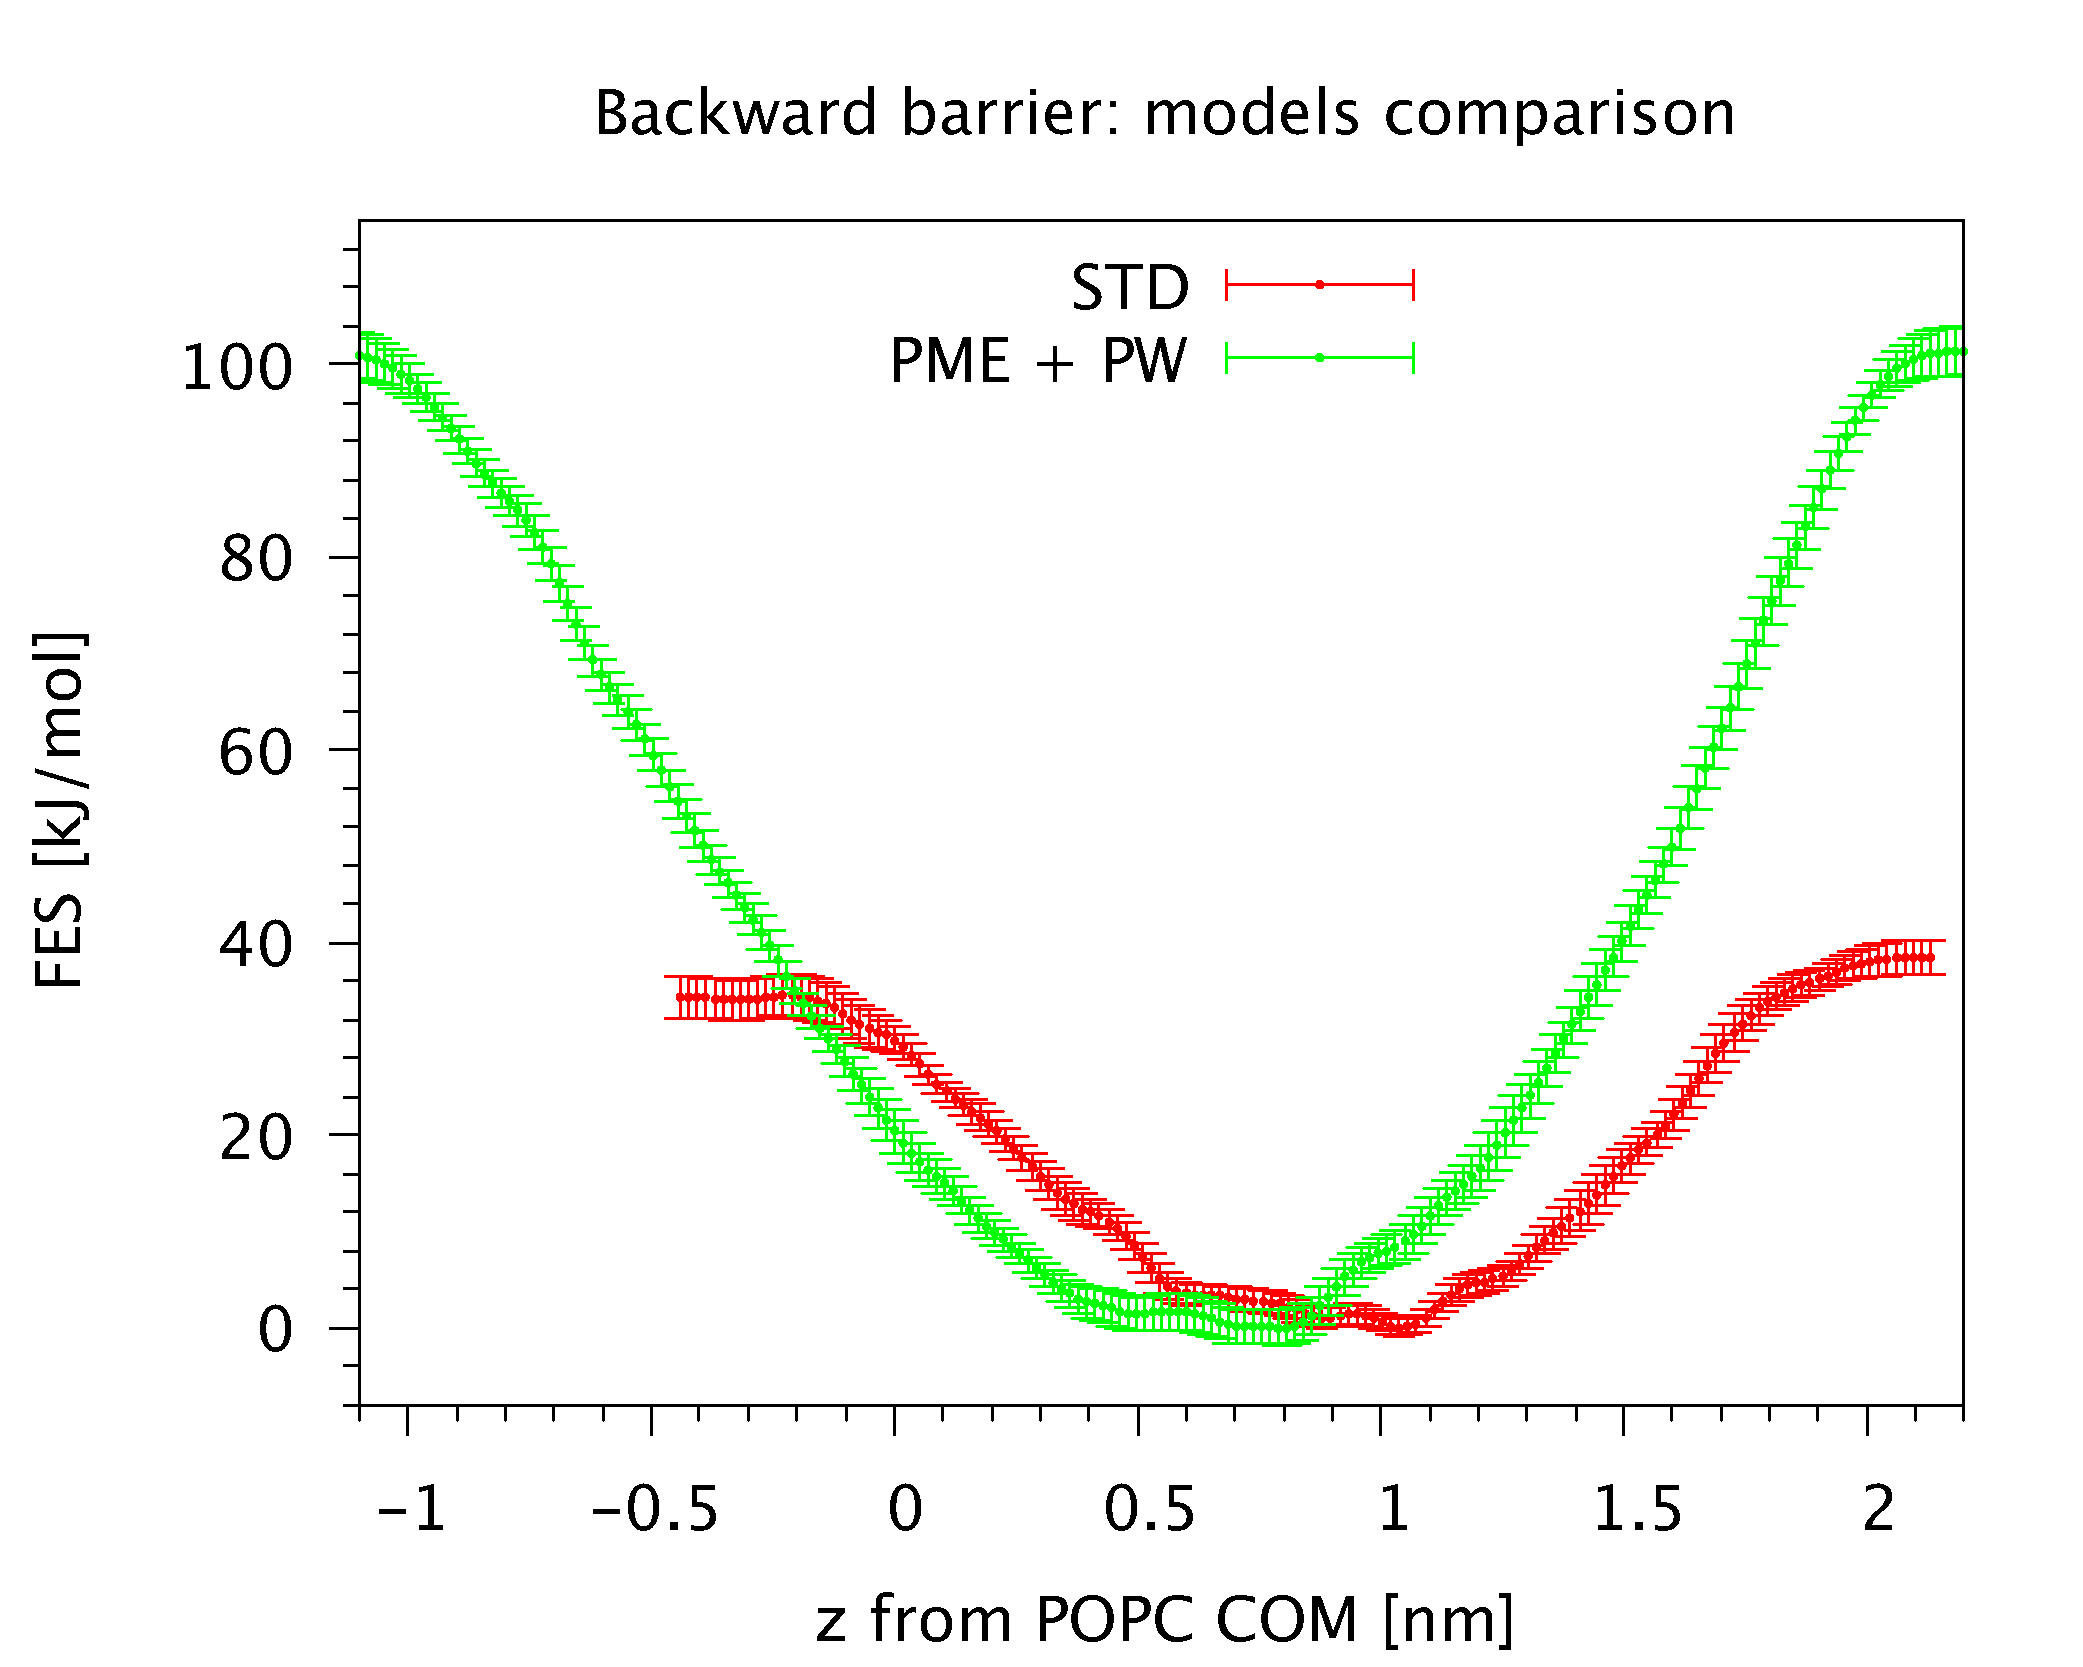
\includegraphics[width=0.5\linewidth]{./img/results/backwardWall}%
		}%
		\subfloat[Random and striped NP comparison]{%
		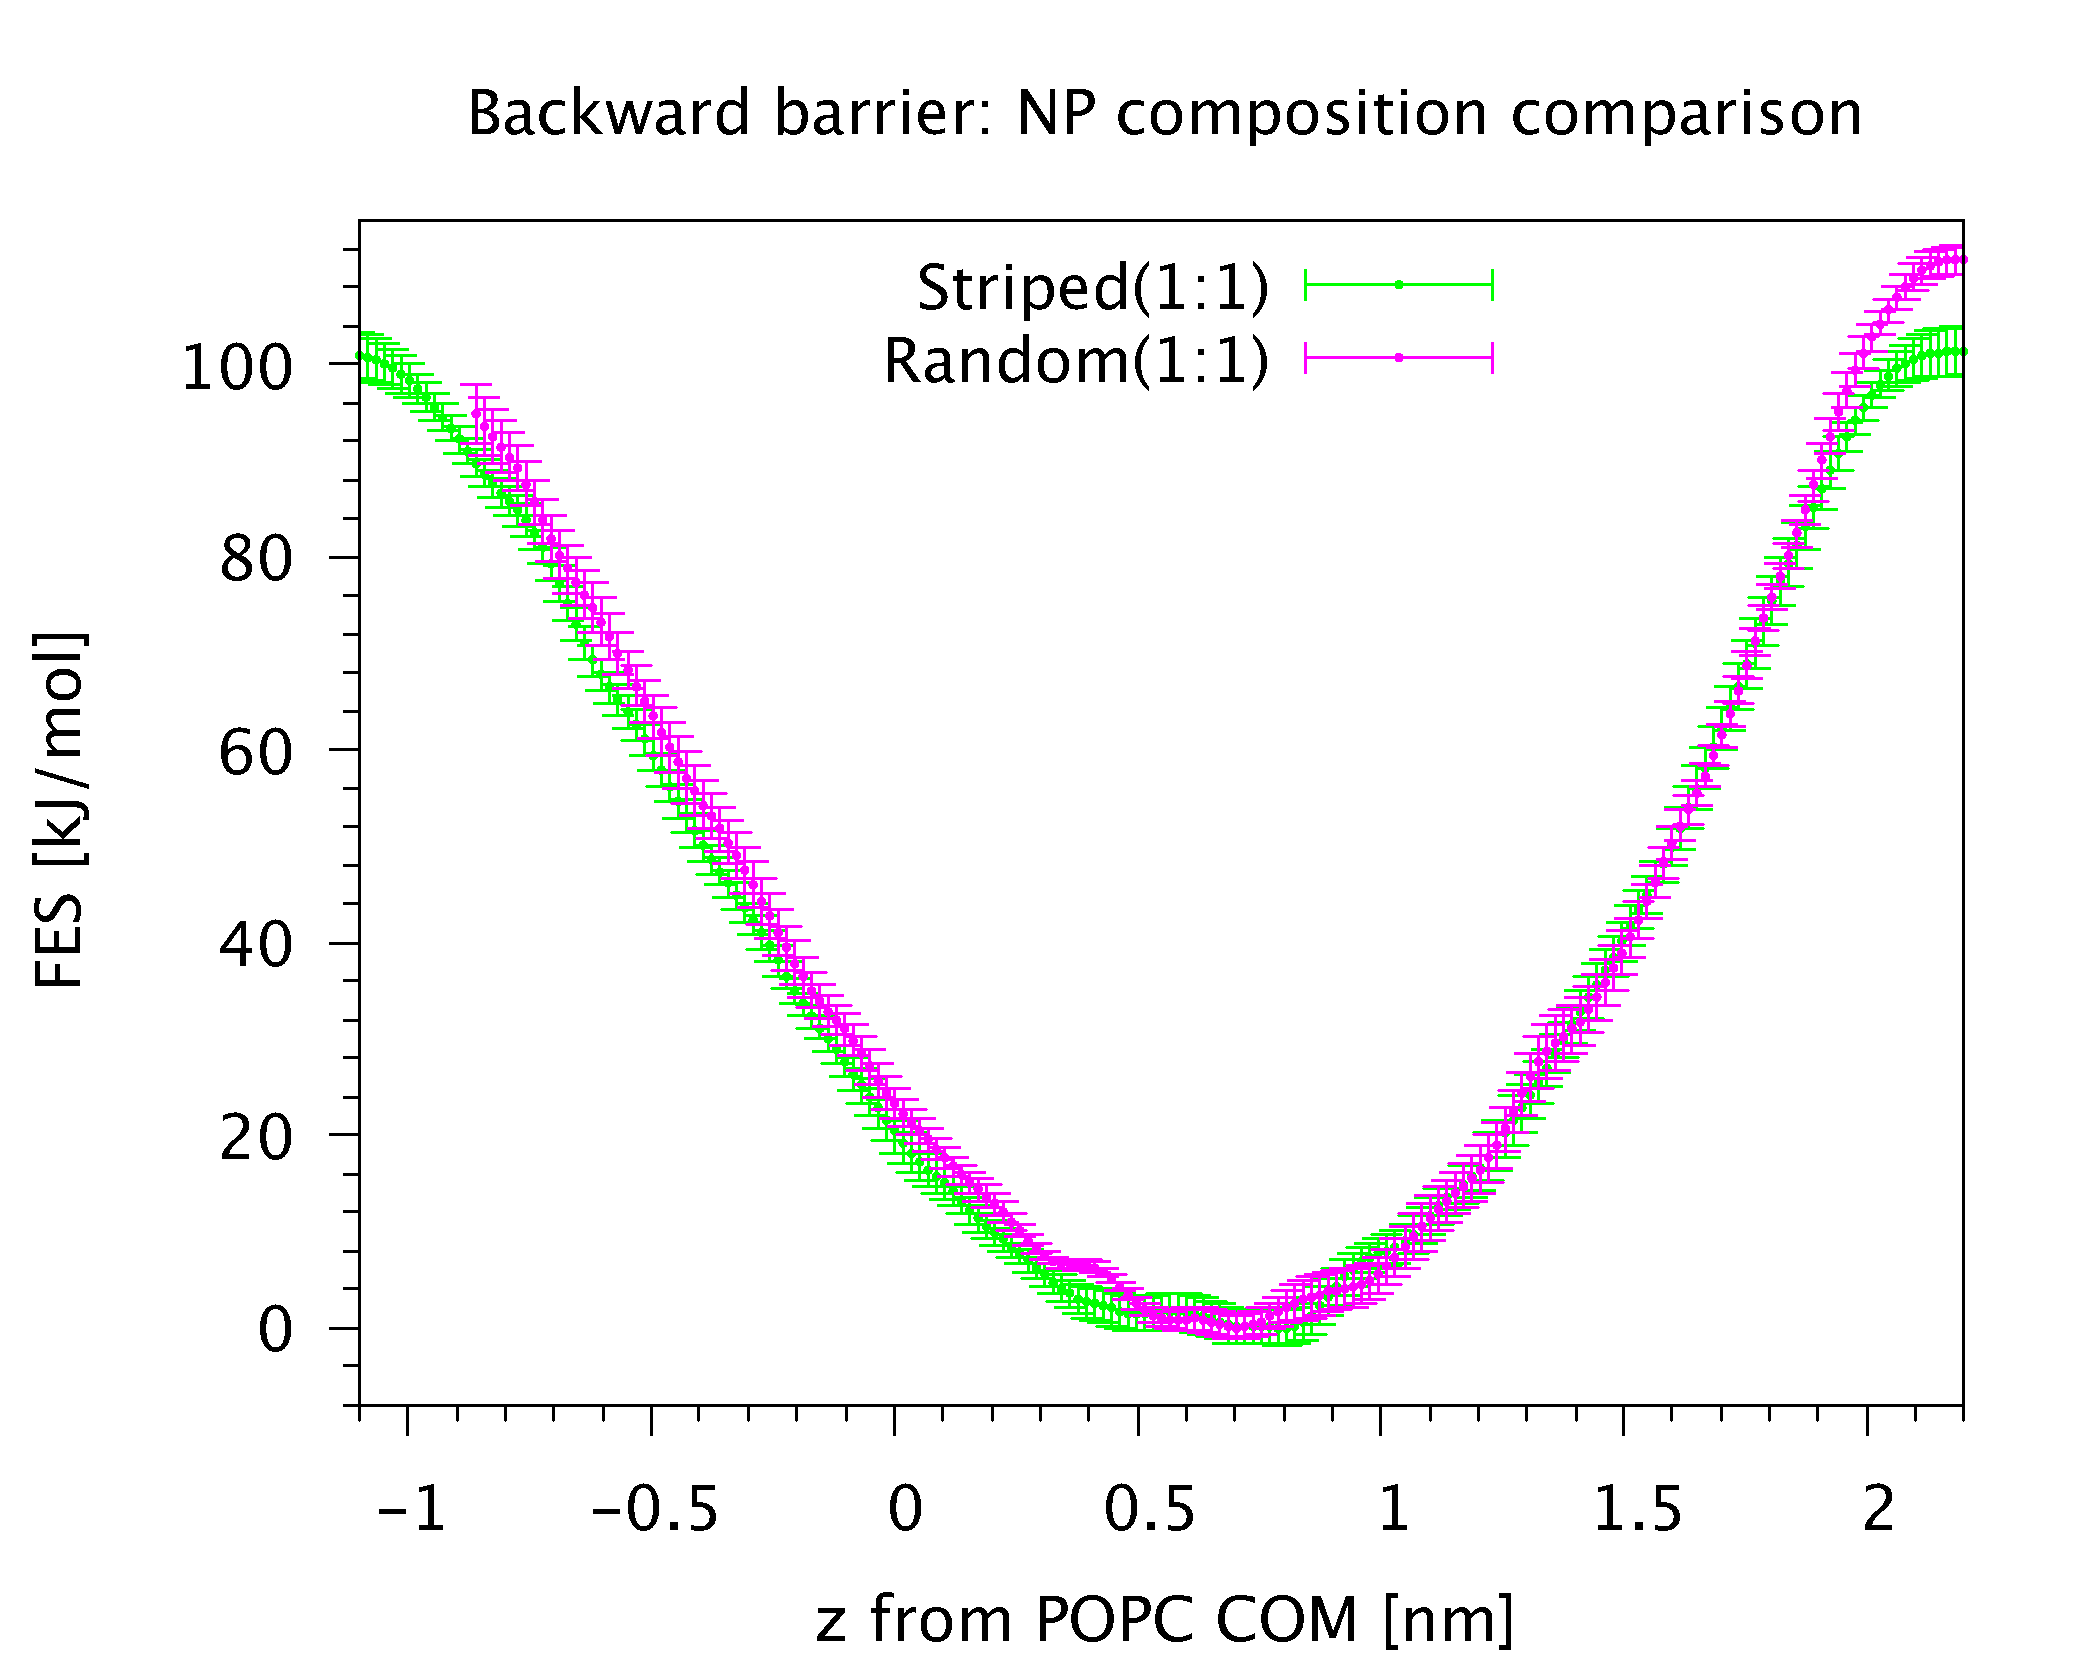
\includegraphics[width=0.5\linewidth]{./img/results/backwardWallRP}%
		}%
		\caption{\acs{FES} of the backward energy barrier as a function of the \acs{CV}. (a) In a comparison with different \acs{CG} models. (b) In a comparison with the striped and the random \acp{NP} with \acs{PME} and \acs{PW}. The data for the STD version are an average over eight runs; for the striped with \ac{PME} and \acs{PW} are an average over eight runs and for the random with \ac{PME} and \acs{PW} are an average over five runs.}%
		\label{fig:backwardWall}
	\end{adjustwidth}
\end{figure}

%\subsection{Striped and random comparison}
The metadynamics runs performed allow us for a comparison of the forward energy barrier for the striped 
(\ac{MUS}:\ac{OT} $1$:$1$) and the random (\ac{MUS}:\ac{OT} $1$:$1$) \acp{NP} with the \ac{PW}. The comparison is 
shown in figure~(\ref{fig:forwardWall}b) and in table~(\ref{tab:hydroTime}). We can confirm the trend observed in 
\cite{ourPaper}: the striped (\ac{MUS}:\ac{OT} $1$:$1$) \ac{NP} has an higher energy barrier for the hydrophobic 
to one anchor state transition than the random (\ac{MUS}:\ac{OT} $1$:$1$) \ac{NP}. Moreover in 
table~(\ref{tab:hydroTime}) we can see that the different height of the energy barriers is reflected by the time 
spent by the two types of \acp{NP} in the hydrophobic state.

\subsection{Backward process}
As for the forward energy wall, the same procedure was followed in order to calculate the backward energy wall. 
This time the metadynamics runs have to start from the anchored state, as an example in 
figure~(\ref{fig:startFrameAnchored}). Since the available machine time, I have performed eight metadynamics runs 
for the striped (\ac{MUS}:\ac{OT} $1$:$1$) \ac{NP} with the \ac{STD} \martini{} models; nine metadynamics runs for 
the striped (\ac{MUS}:\ac{OT} $1$:$1$) \ac{NP} with \ac{PME} and \ac{PW} and five metadynamics runs for the random 
(\ac{MUS}:\ac{OT} $1$:$1$) \ac{NP} with \ac{PME} and \ac{PW}. The achieved results are shown in 
figure~(\ref{fig:backwardWall}).
\begin{table}[h!t]
	\centering
	\begin{tabular}{lcccc}
		\toprule
		\,					& striped($1$:$1$)	& striped($1$:$1$)	& random($1$:$1$)	\\
		\,					& STD & \acs{PME}$+$\acs{PW} & \acs{PME}$+$\acs{PW} \\ \toprule
	$\overline{t_{a}}$ [ns]	& $\sim 156$	& $\sim 607$	& $\sim 680$	\\ \midrule
	$\Delta G$ [kJ/mol] 	& $34 \pm 3$ 	& $100 \pm 4$ 	& $95 \pm 4$	\\ \bottomrule
	\end{tabular}
	\caption{Summary of the metadynamics results for the striped and the random \acp{NP} for the backward process. $\overline{t_a}$ is average time spent by the \acs{NP} in the anchored state. $\Delta G$ is the average height of the backward energy wall. The error is the standard error of the mean value. Data obtained from my \acs{MD} runs.}%
	\label{tab:anchorTime}
\end{table}

\begin{SCfigure}[][!ht]
	\centering
	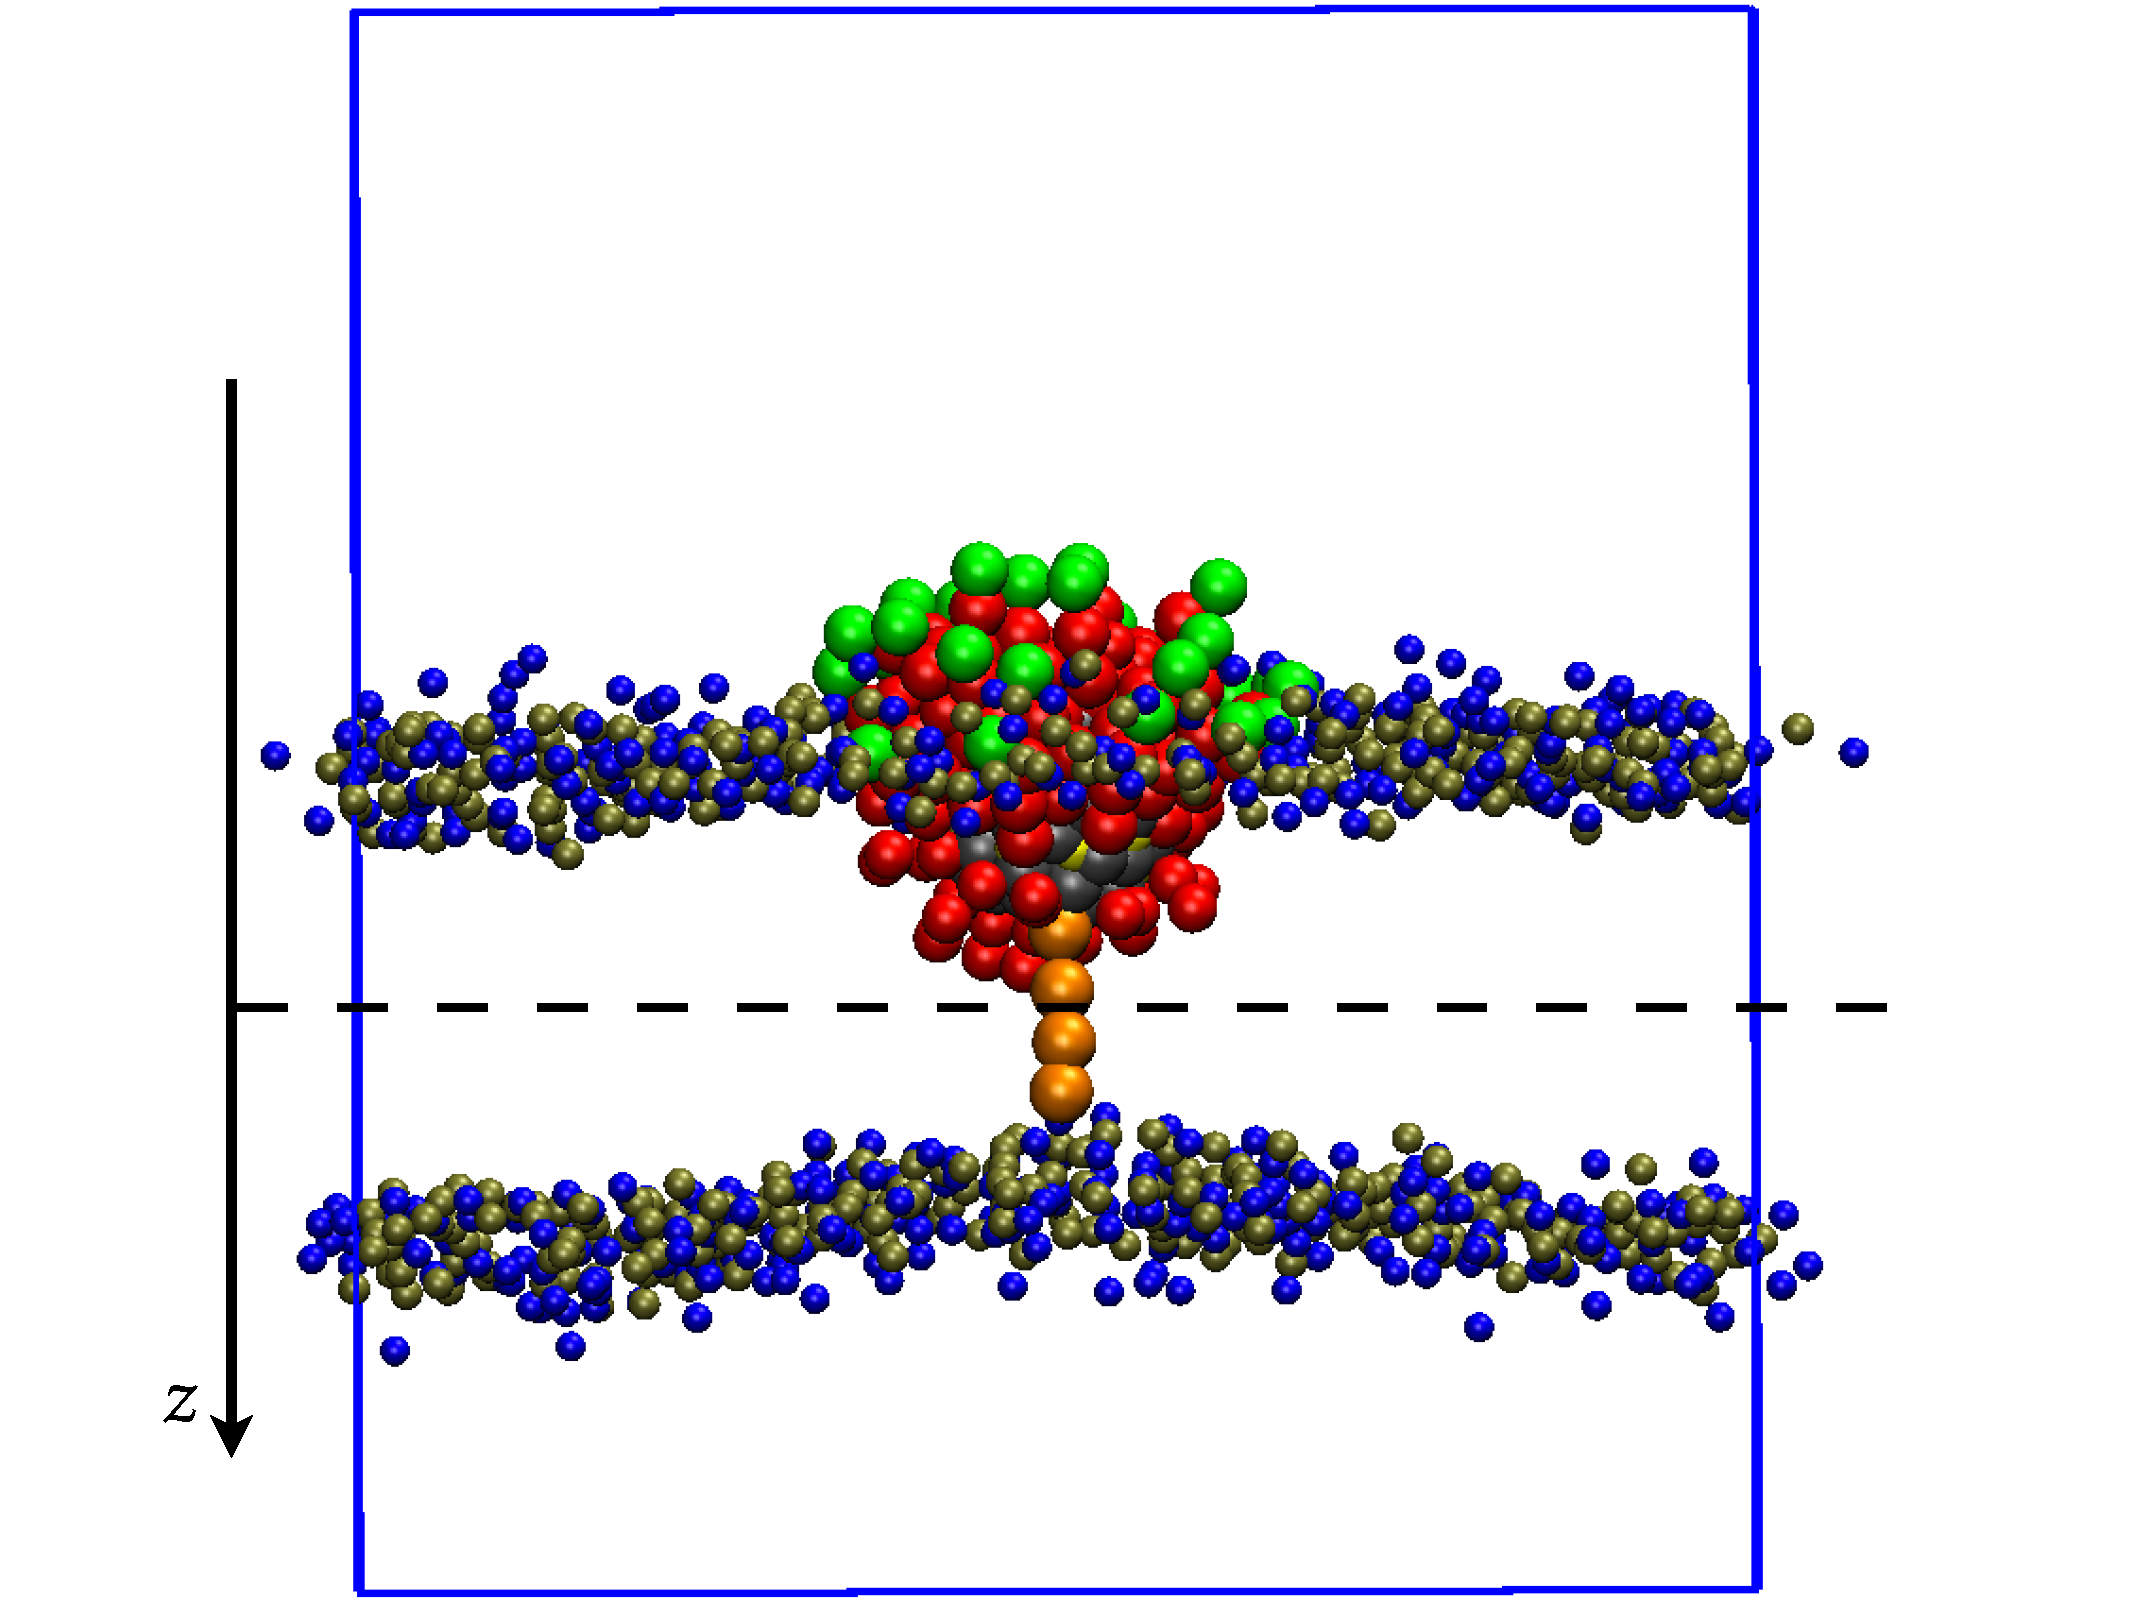
\includegraphics[width=0.44\textwidth]{./img/patchedAnchored.pdf}
	\caption{Example of a starting frame of a metadynamics run of a striped (\ac{MUS}:\ac{OT} $1$:$1$) \ac{NP} in a one anchor state. Color code as in figure~(\ref{fig:threeProcess}). The charged ligand chosen for the anchoring process is in orange. The dashed line is the center of the bilayer. The blue contour is the simulation box. Water beads and lipid tails are not shown.}%
	\label{fig:startFrameAnchored}
\end{SCfigure}

This results suggest that the for- and backward processes for the striped \ac{NP} are more similar and symmetrical 
to each other than what is observed in \cite{ourPaper}. The random \ac{NP}, instead, shows a more stable 
configuration in the anchored state since the backward energy wall is higher for the random \ac{NP} then that for 
the striped one.

In table~(\ref{tab:anchorTime}) is shown the energy wall and the average time spent by the \ac{NP} in the anchored 
state in a comparison between different models and configurations.

\subsection{Discussion of the results}
The process of the charged ligand translocation through the membrane can be thermodynamically compared to two 
other relevant processes for biological membranes: the ion membrane translocation and the lipid flip--flopping.

For the first comparison, in \cite{PW} the authors have computed the \ac{FES} of the translocation of one Na$^+$ 
and one Cl$^-$ ion across a \acs{DPPC} membrane using umbrella sampling and the \ac{WHAM} procedure with the 
\ac{STD} \martini{} \ac{FF}. The calculations were performed with the \ac{PW} alone and with \ac{PW}$+$\ac{PME}. 
The height of the barriers are reported in table~(\ref{tab:ionTranslocation}). The same \ac{FES} for a \acs{DMPC} 
membrane was calculated by Khavrutskii \etal{} \cite{atomisticTranslocation} with an atomistic \ac{FF}. Since the 
\martini{} model for the \acs{DPPC} lipid also model the \acs{DMPC} lipid a comparison can be made and it is shown 
in table~(\ref{tab:ionTranslocation}). As one can see, from left to right, increasing the accuracy of the 
treatment of the electrostatic interactions the \martini{} \ac{FF} approaches the results of the atomistic 
\ac{FF}, as we have observed for the charged ligand translocation, see figure~(\ref{fig:forwardWall}). Moreover, 
the energy barrier for ion translocation is quantitatively comparable to those we have calculated for the forward 
and backward translocation of the charged ligand.
%Moreover in \cite{PW}, in accordance with the atomistic results in \cite{atomisticTranslocation}, for small cross membrane ions imbalance and only with the use of the \ac{PW} model and the \ac{PME} method, they observe some ion leakage without pore formation but still mediated by a water defect inside the membrane, called \textit{water finger} that help the ions to cross the hydrophobic region of the membrane.
%We remark that, these kind of phenomena, are totally absent using the \ac{STD} \martini{} \ac{FF}. Hence, as already outlined, the importance to use a better treatment of the electrostatic interaction and a better model for water solvent.
\begin{table}[h!t]
	\centering
	\begin{tabular}{lcccc}
		\toprule
		\,		& STD$^a$ 	& \acs{PW}$^a$ 	& \acs{PW}$+$\acs{PME}$^a$ 	& atomistic$^b$	\\ \toprule
		Na$^+$	& $68.0$& $67.6$	& $78.6$	& $91.7$ 	\\ \midrule
		Cl$^-$	& $69.2$& $70.4$	& $99.0$	& $98.8$	\\ \bottomrule
	\end{tabular}
	\caption{Height of the energy barrier (in kJ/mol) for Na$^+$ and Cl$^-$ ion translocation across a bilayer. $^a$ Results based on a \acs{DPPC} membrane, taken from \cite{PW}. $^b$ Results based on a \acs{DMPC} membrane, taken from \cite{atomisticTranslocation}.}%
	\label{tab:ionTranslocation}
\end{table}

For the second comparison, we refer to the work of Sapay \etal{} in \cite{Sapay2009}, in which the authors have 
calculated, using an atomistic \ac{FF} and through umbrella sampling, the \acp{FES} of a flip--flopping process of 
a lipid in several pure bilayers with different lipid composition, including a pure \ac{POPC} membrane. They pull 
a lipid head inside the hydrophobic core via a bias potential and found that the energy barrier of a lipid 
flip--flop in a \ac{POPC} membrane is of the order of $\sim 90$~kJ/mol. Moreover they observe that the 
flip--flopping process occurs without a water pore formation, as in our case: the  ligand translocation occurs 
without a pore formation. Maybe this kind of comparison is more realistic than the previous one. This because the 
charged ligand has an hydrophobic chain, like a lipid, and because, the ions penetrate the membrane from the water 
phase while our ligand starts in the lipid heads region of the entrance leaflet and in most cases the hydrophobic 
beads are already in contact with the hydrophobic region of the membrane. Instead, there is an important 
difference: the lipid has a natural polar head while the ligand is charged.

\section{Molecular description of the process}
\label{sec:resultsUnBiased}
%Introduzione a seguito dei risultati con la metadinamica: run unbiased con PW striped, random11, random 12 e POPC
In the previous paragraphs we have characterized the anchoring and dis--anchoring process from a thermodynamic 
point of view. In the following we will instead focus on the molecular processes that occur during anchoring and 
dis--anchoring.

To this aim, we will analyze both biased (via metadynamics) and unbiased \ac{MD} trajectories. We remark that the 
unbiased \ac{MD} simulations we have performed with the \ac{PW}+\ac{PME} model concern the \ac{NP} in the 
hydrophobic state only. Indeed, the high energy barriers that need to be overcome to get to the anchored state 
make the spontaneous anchoring process too slow to be observed on the microsecond time scale. Unbiased \ac{MD} 
simulations are nevertheless useful to characterize the hydrophobic state in absence of any biasing potential.

% In view of the results obtained with metadynamics, shown in the previous chapter, and in order to try to see the anchoring process to spontaneously occur, we decide to perform unbiased runs starting from the hydrophobic state for all the anionic \ac{AuNP} configurations: the striped (\ac{MUS}:\ac{OT} $1$:$1$), the random (\ac{MUS}:\ac{OT} $1$:$1$) and the random (\ac{MUS}:\ac{OT} $2$:$1$), with both \ac{PME} and \ac{PW} model. This runs are suitable to get some useful information about the molecular processes involved and about the hydrophobic state with a more realistic \ac{CG} description.
%
% Unfortunately, with ten of microseconds for each configurations, we have not seen any anchoring process. This confirm, in accordance with the atomistic model and the metadynamics results, the increase of the energy barrier respect to the \ac{STD} \martini{} model and the slowdown of the dynamics of the system. Despite this, the unbiased runs are useful in order for a comparison with the metadynamics runs to be made. In particular we can compare some interesting molecular phenomena that we have see in metadynamics runs such as: the dragging of the water bead inside the hydrophobic region of the membrane by the charged bead during the anchoring process; the choline group bead of the entrance leaflet dragged inside the hydrophobic region by the charged bead during the anchoring process and the engulfment effect of the opposite leaflet during the dis--anchor process. Moreover, comparing the results of the hydrophobic state only, we can get some information about the destructiveness of the metadynamics and if and how the bilayer properties change.

\subsection{Water dragging}
\label{sec:WDragging}
%Trascinamento delle PW nelle varie salse
In order to quantify the amount of water dragged within the membrane core during the charged ligand translocation, 
I calculated the number of contacts between the (biased) charged ligand terminal and the solvent particles. At 
\ac{CG} level, I considered two beads to be in contact whenever their distance was found to be shorter than 
$0.6$~nm. In figure~(\ref{fig:PWDragging}) it is shown an example of the dragging effect for a metadynamics run of 
a striped \ac{NP} with \ac{PME}$+$\ac{PW} while in figure~(\ref{fig:WContact}) the number of ligand--water 
contacts are plotted as a function of the $z$ distance between the charged ligand terminal and the \ac{COM} of the 
membrane. In particular, in figure~(\ref{fig:WContact}a) it is shown a comparison between different \ac{CG} 
\martini{} models: the \ac{STD}, with \ac{PME} alone and with both \ac{PME}$+$\ac{PW}. Instead, in 
figure~(\ref{fig:WContact}b) it is shown a comparison between the striped and the random \acp{NP} with both 
\ac{PME}$+$\ac{PW}. For the number of contacts with the \ac{PW} bead, since the ligand is negatively charged, only 
the contacts with the $WP$ particle of the \ac{PW} bead are considered.
%	WPatchedComparison		WRPComparison
\begin{figure}[!ht]
	\center
	\subfloat[]{%
		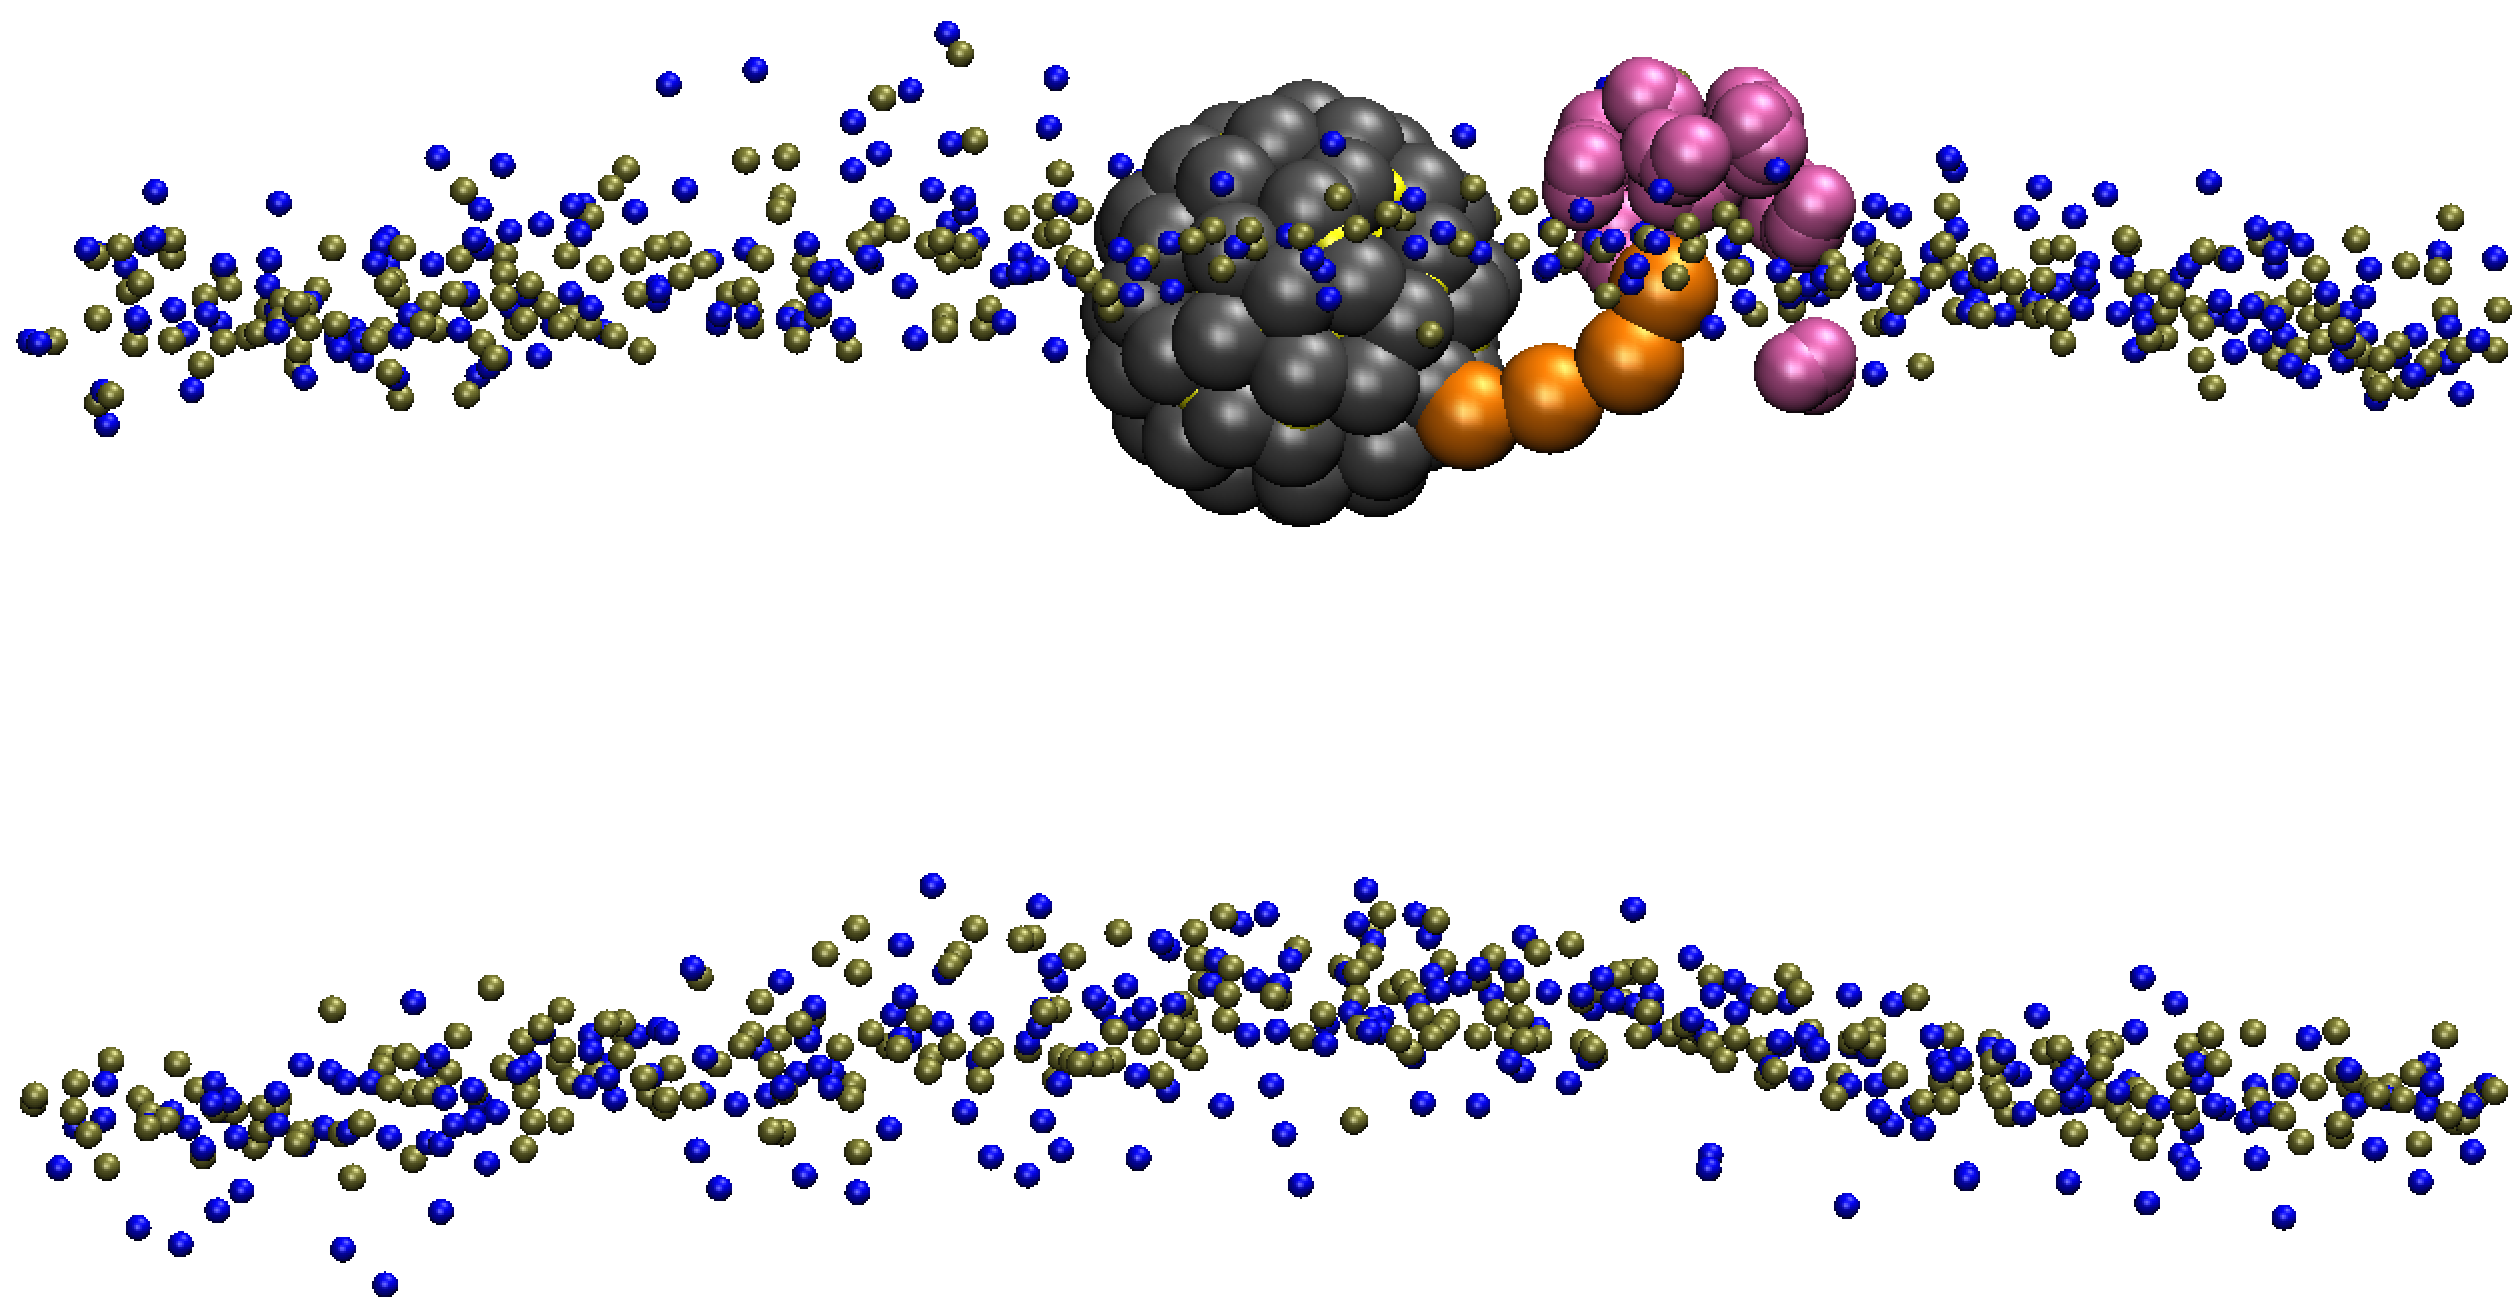
\includegraphics[width=0.47\textwidth]{./img/NC3PWFrame/PWa.png}%
	}\ %
	\subfloat[]{%
		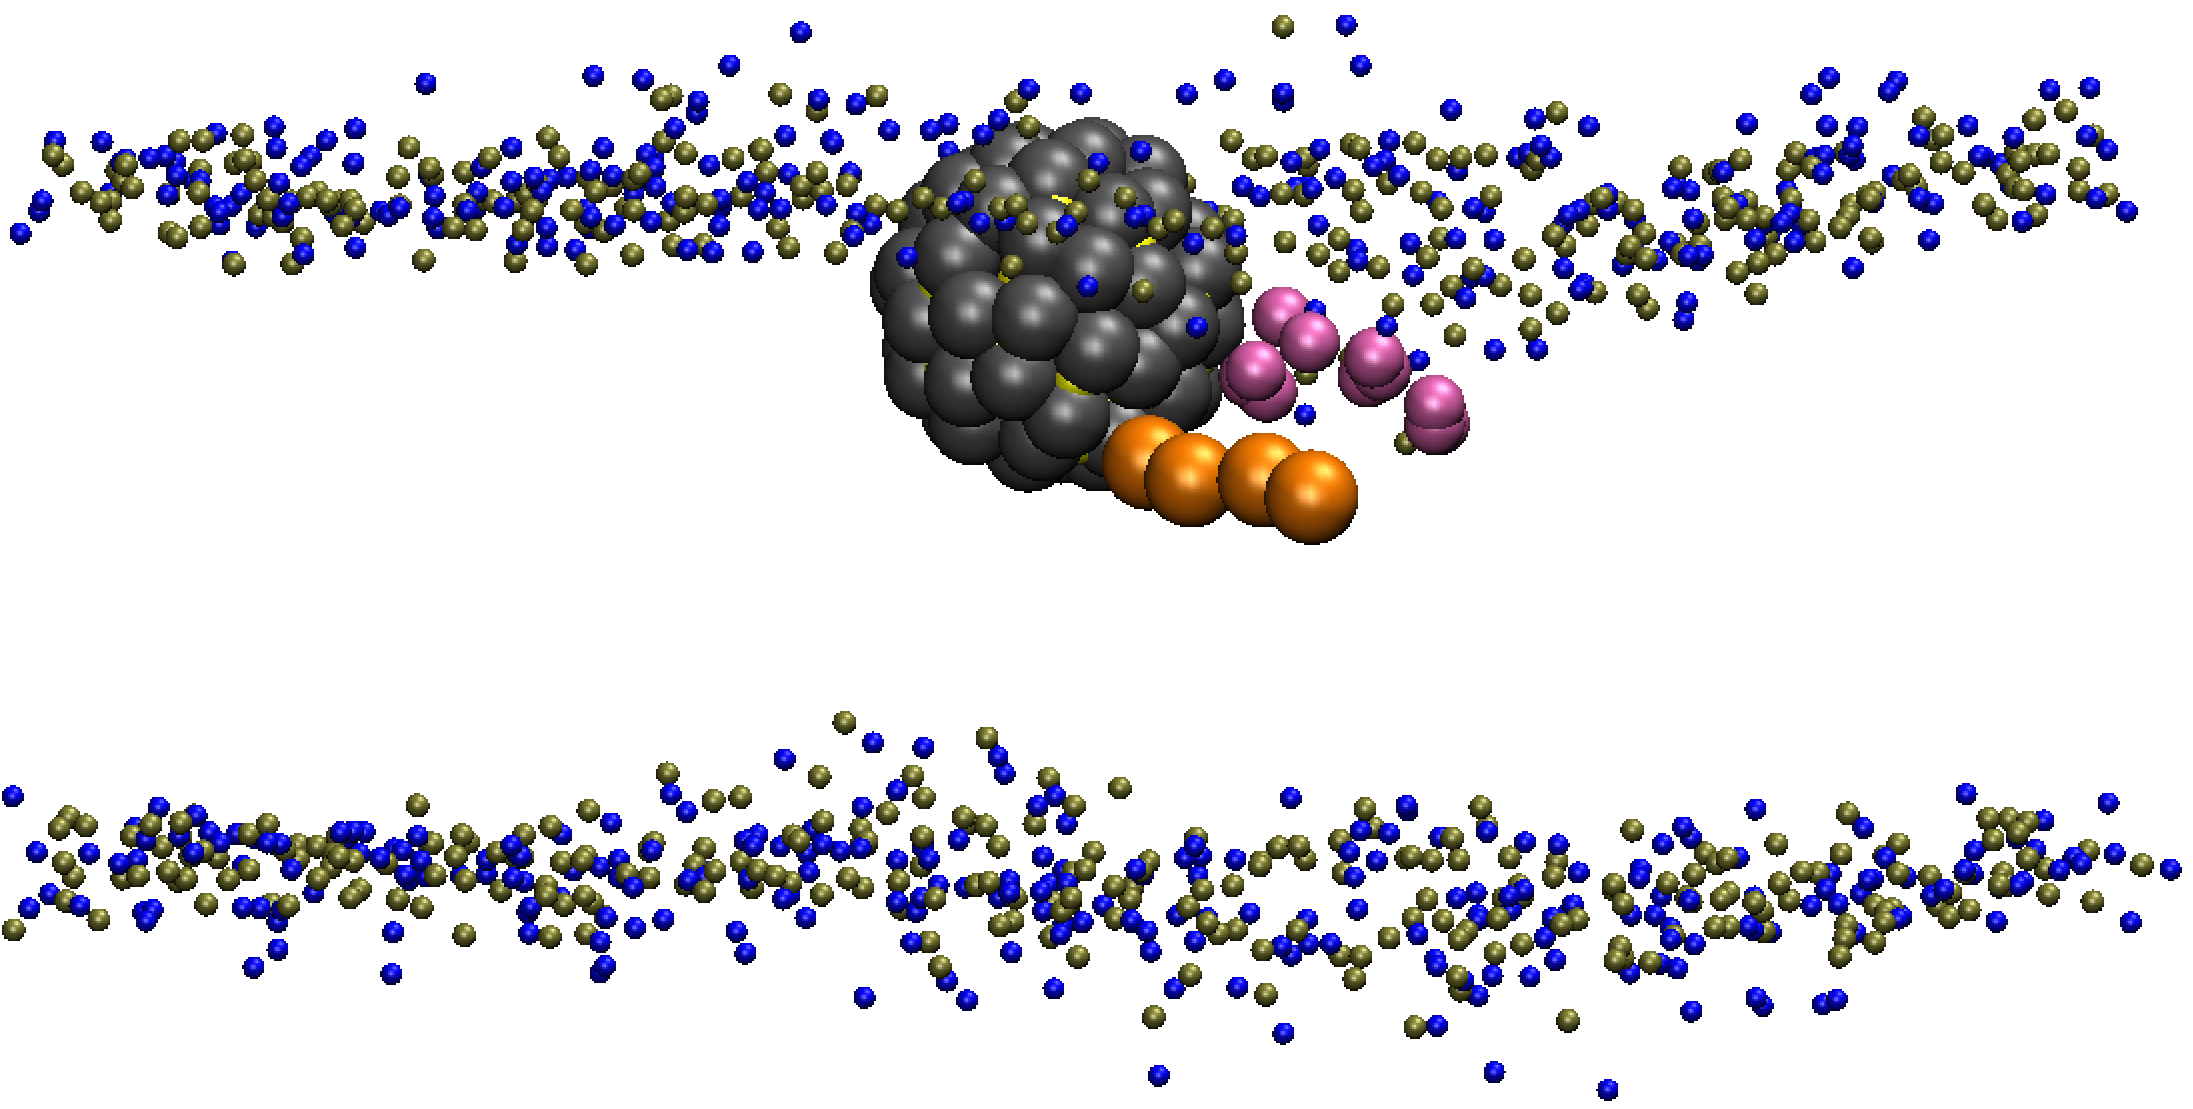
\includegraphics[width=0.47\textwidth]{./img/NC3PWFrame/PWb.png}%
	}\\\medskip%
	\subfloat[]{%
		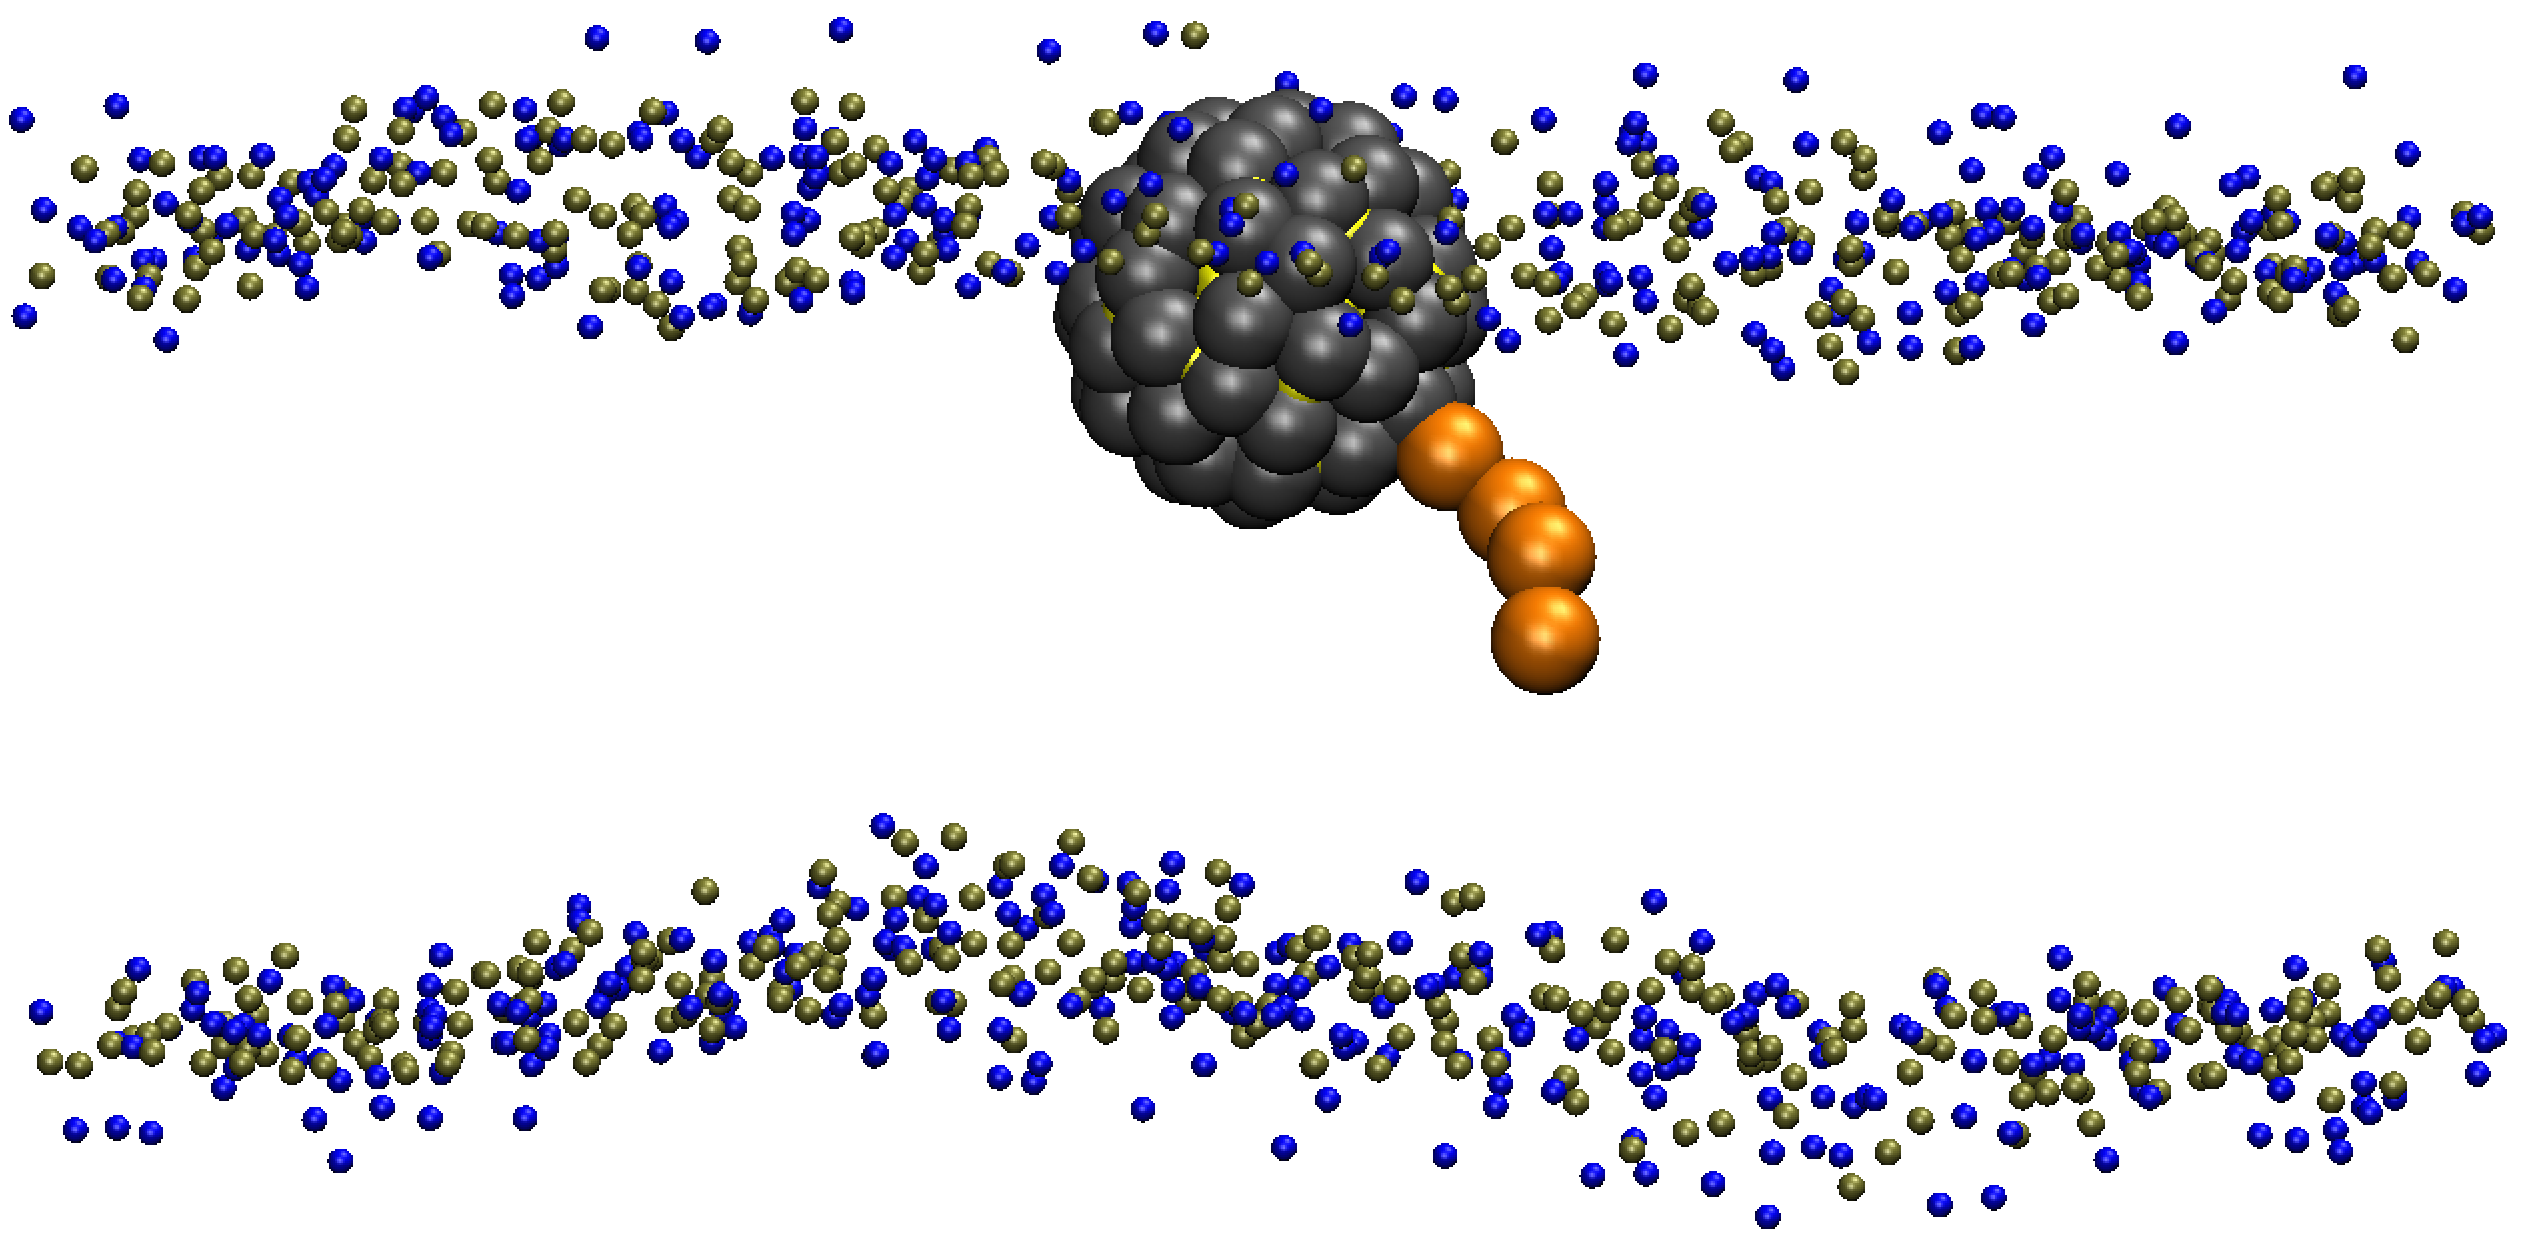
\includegraphics[width=0.47\textwidth]{./img/NC3PWFrame/PWc.png}%
	}\ %
	\subfloat[]{%
		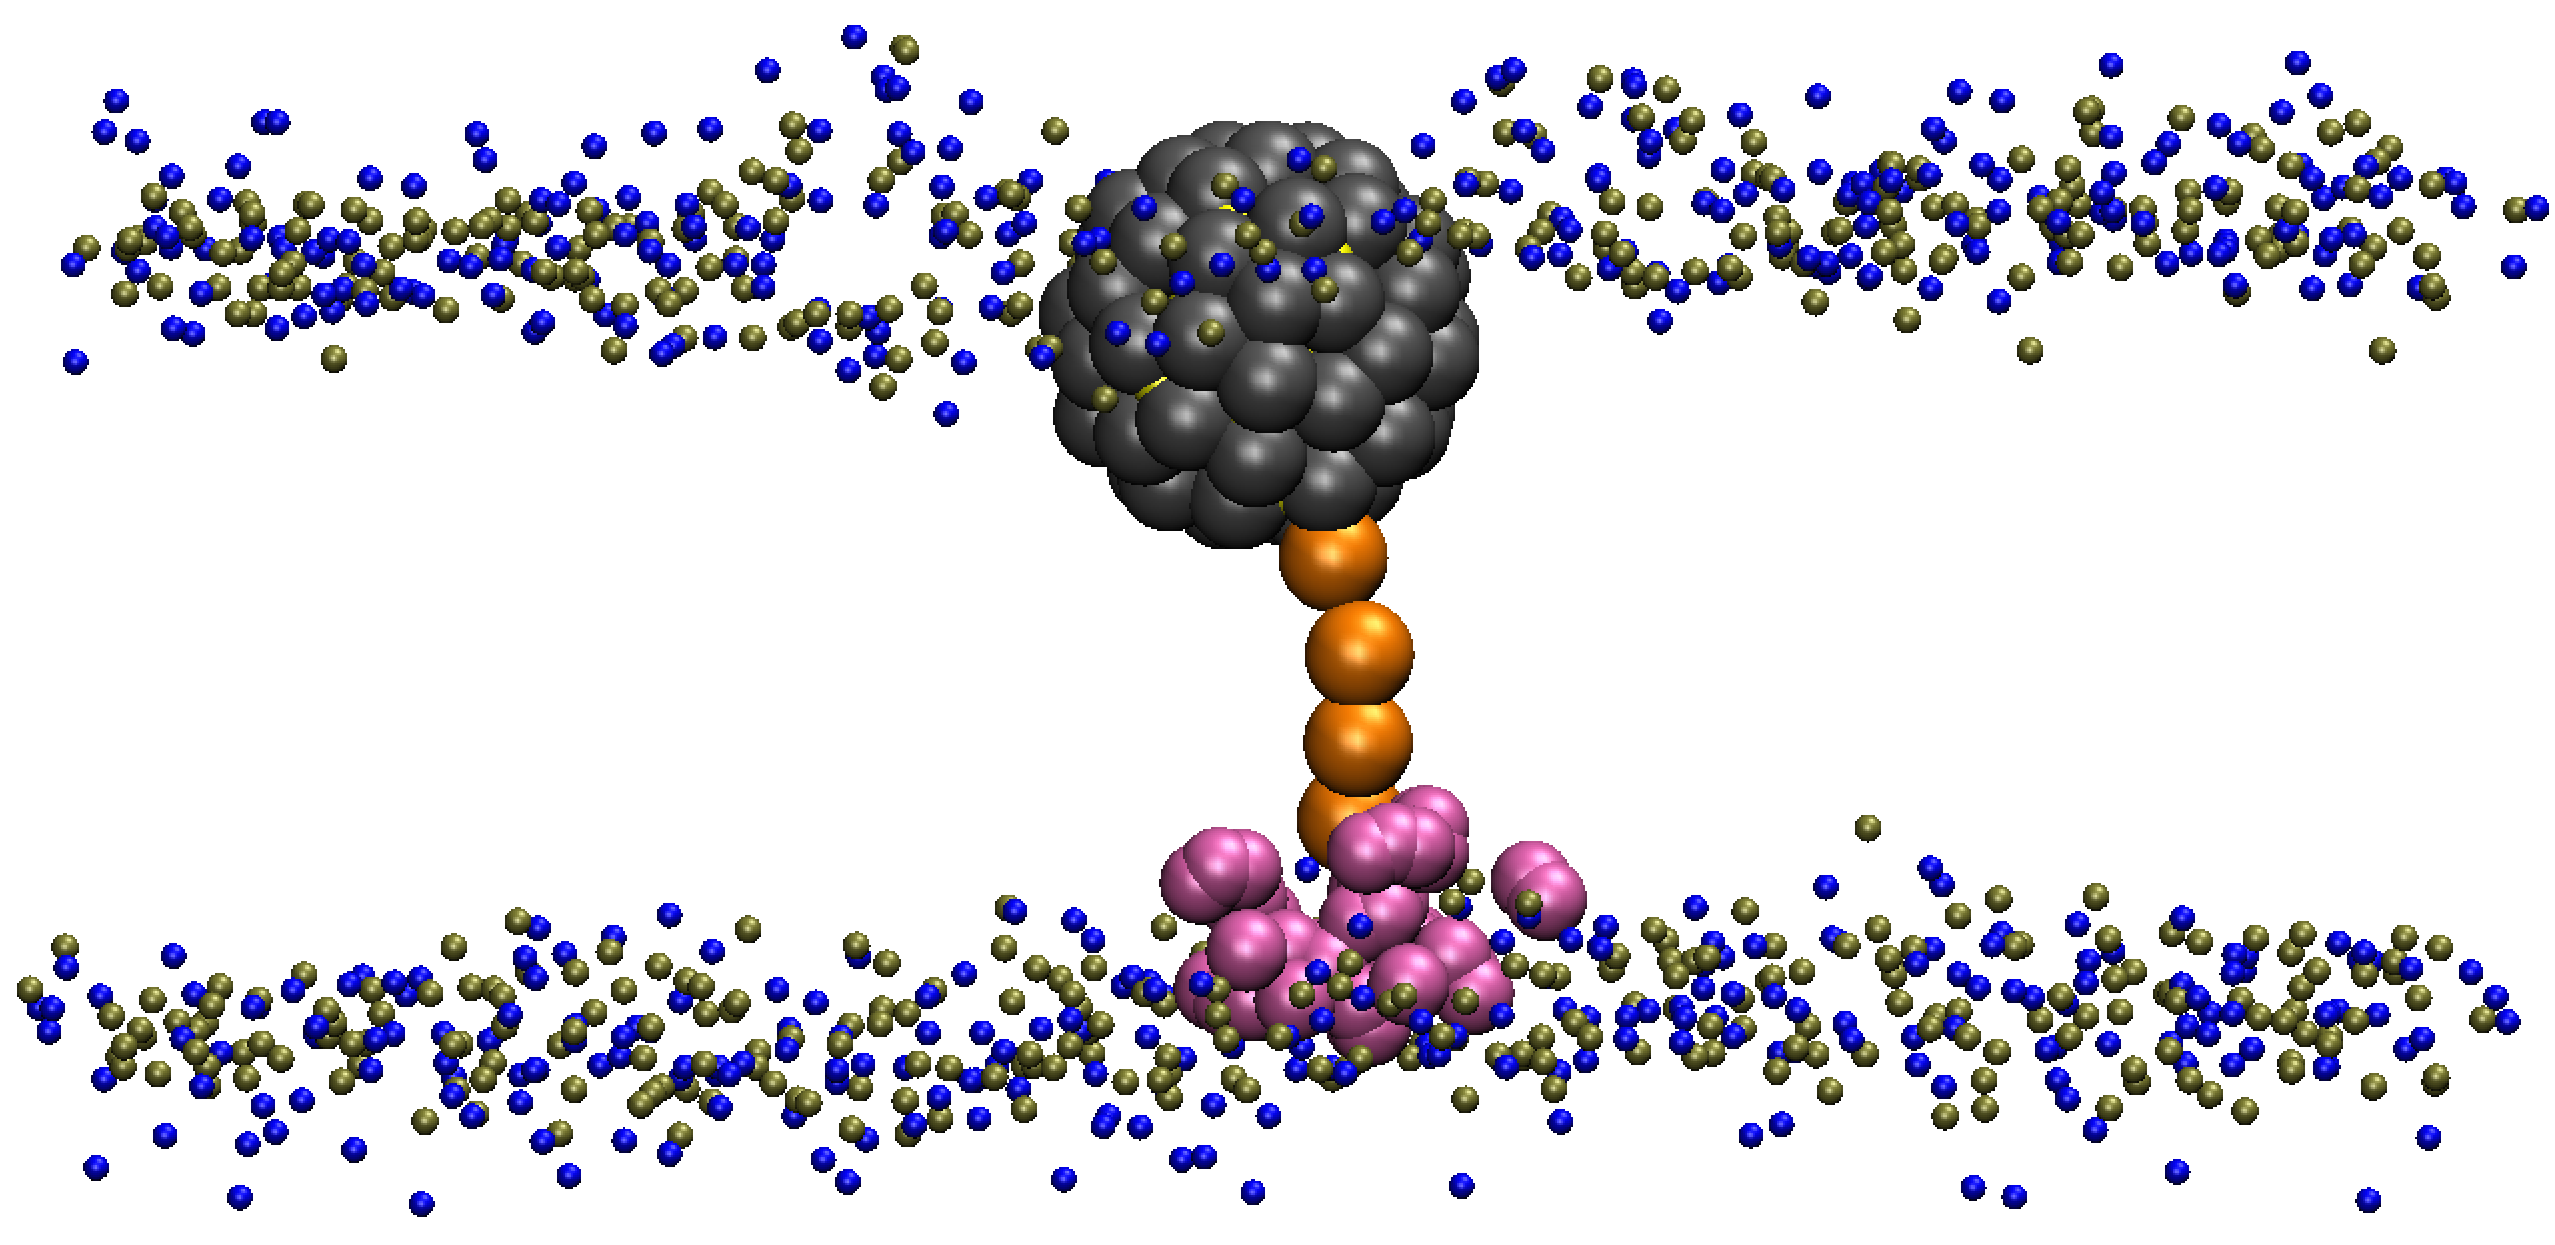
\includegraphics[width=0.47\textwidth]{./img/NC3PWFrame/PWd.png}%
	}\\\medskip%
	\subfloat[]{%
		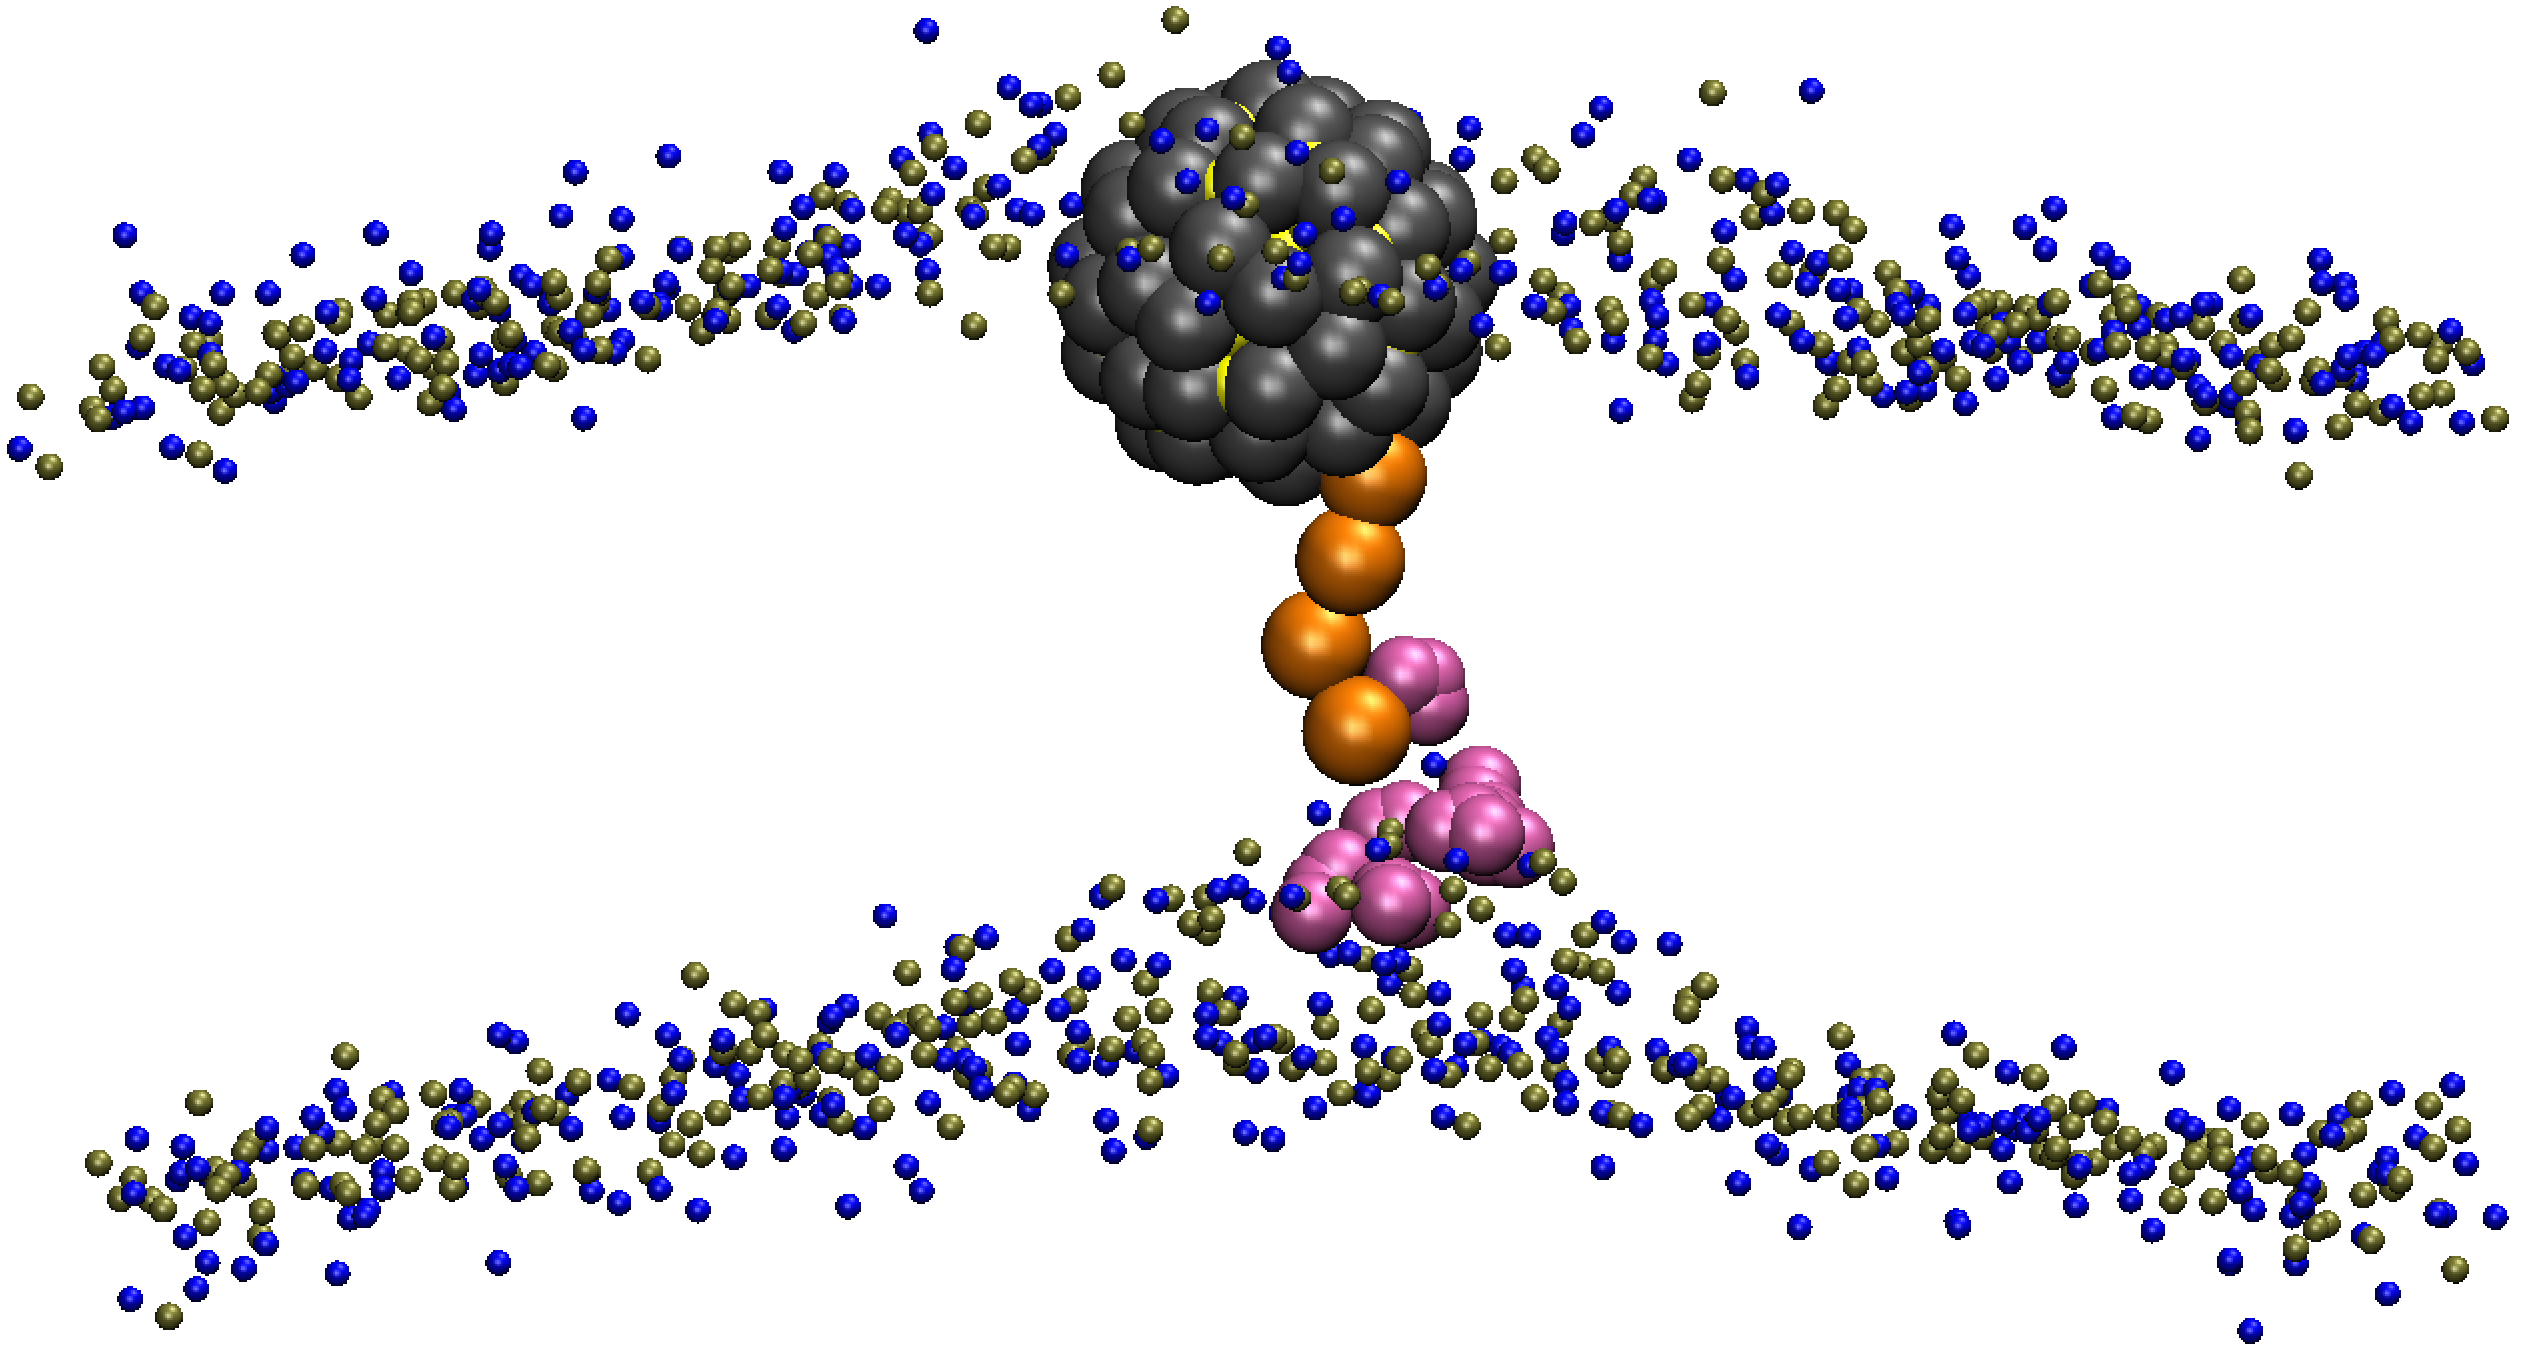
\includegraphics[width=0.47\textwidth]{./img/NC3PWFrame/PWe.png}%
	}\ %
	\subfloat[]{%
		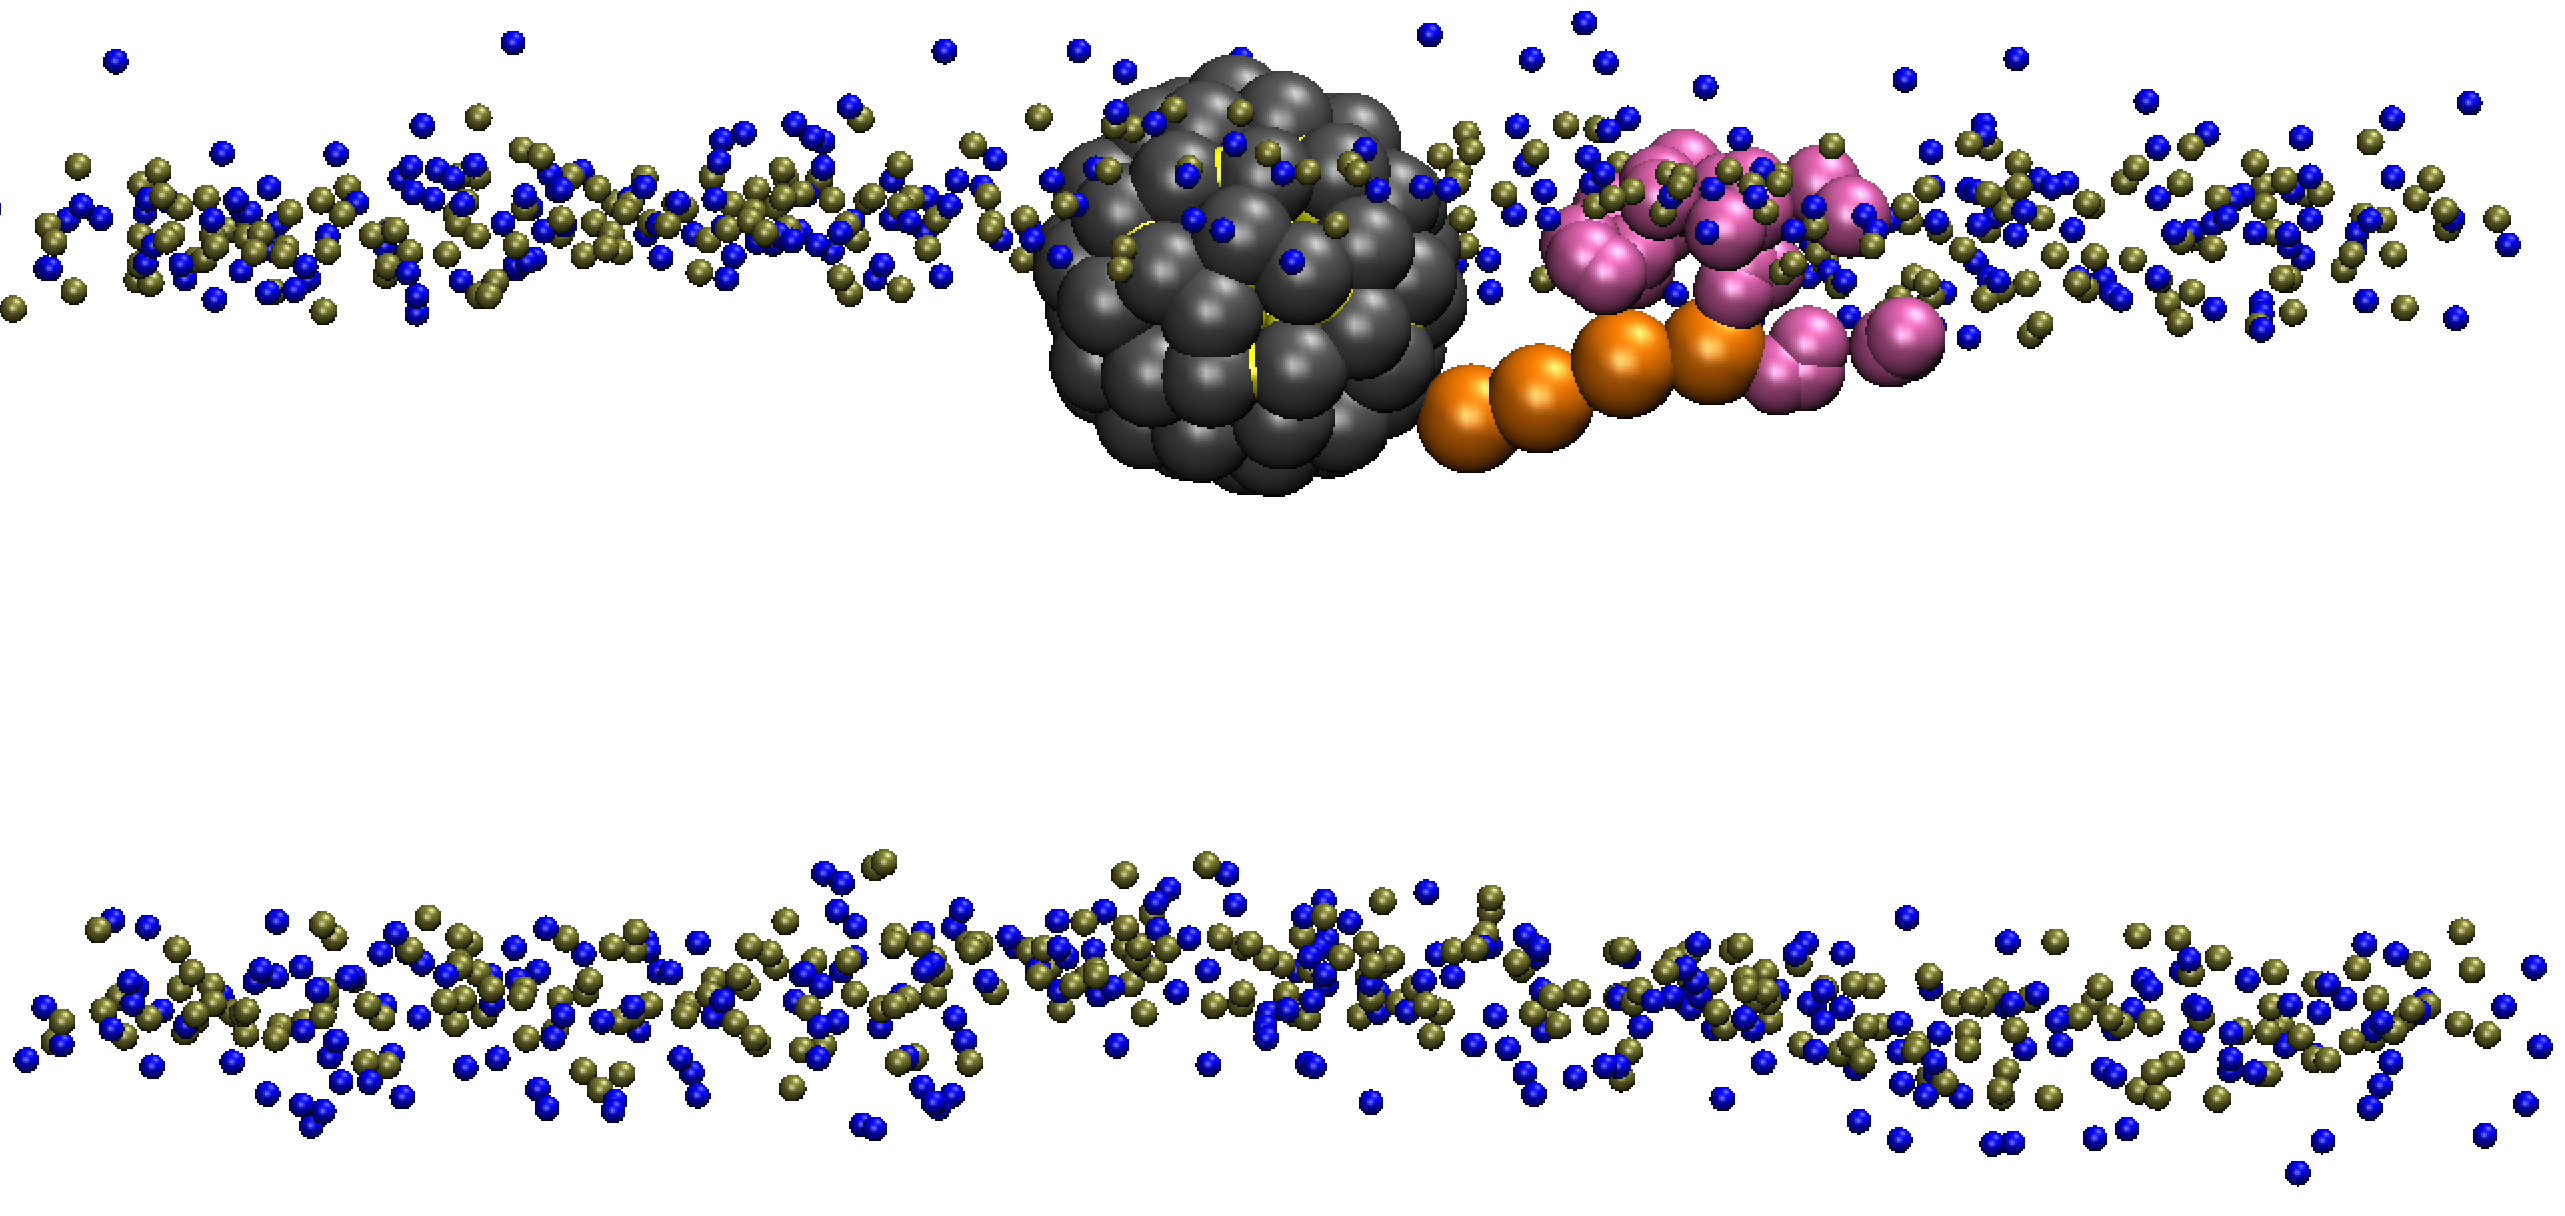
\includegraphics[width=0.47\textwidth]{./img/NC3PWFrame/PWf.png}%
	}%
	\caption{Same frames of figure~(\ref{fig:metaFrame}) in which the water dragging effect is shown. We see that when the ligand approaches the opposite leaflet or when it tries to dis--anchor some \acs{PW} beads penetrate inside the membrane. But when the ligand is in the core of the membrane (c), no water beads are present. Color code as in figure~(\ref{fig:threeProcess}). The charged ligand chosen for the metadynamics is in orange. Water beads (pink) are not shown except for those in contact with the charged ligand terminal. Lipid tails and the other \acs{NP} ligands are not shown.}%
	\label{fig:PWDragging}
\end{figure}
\begin{figure}[ht!]
	\center
	\subfloat[Striped NP: models comparison]{
		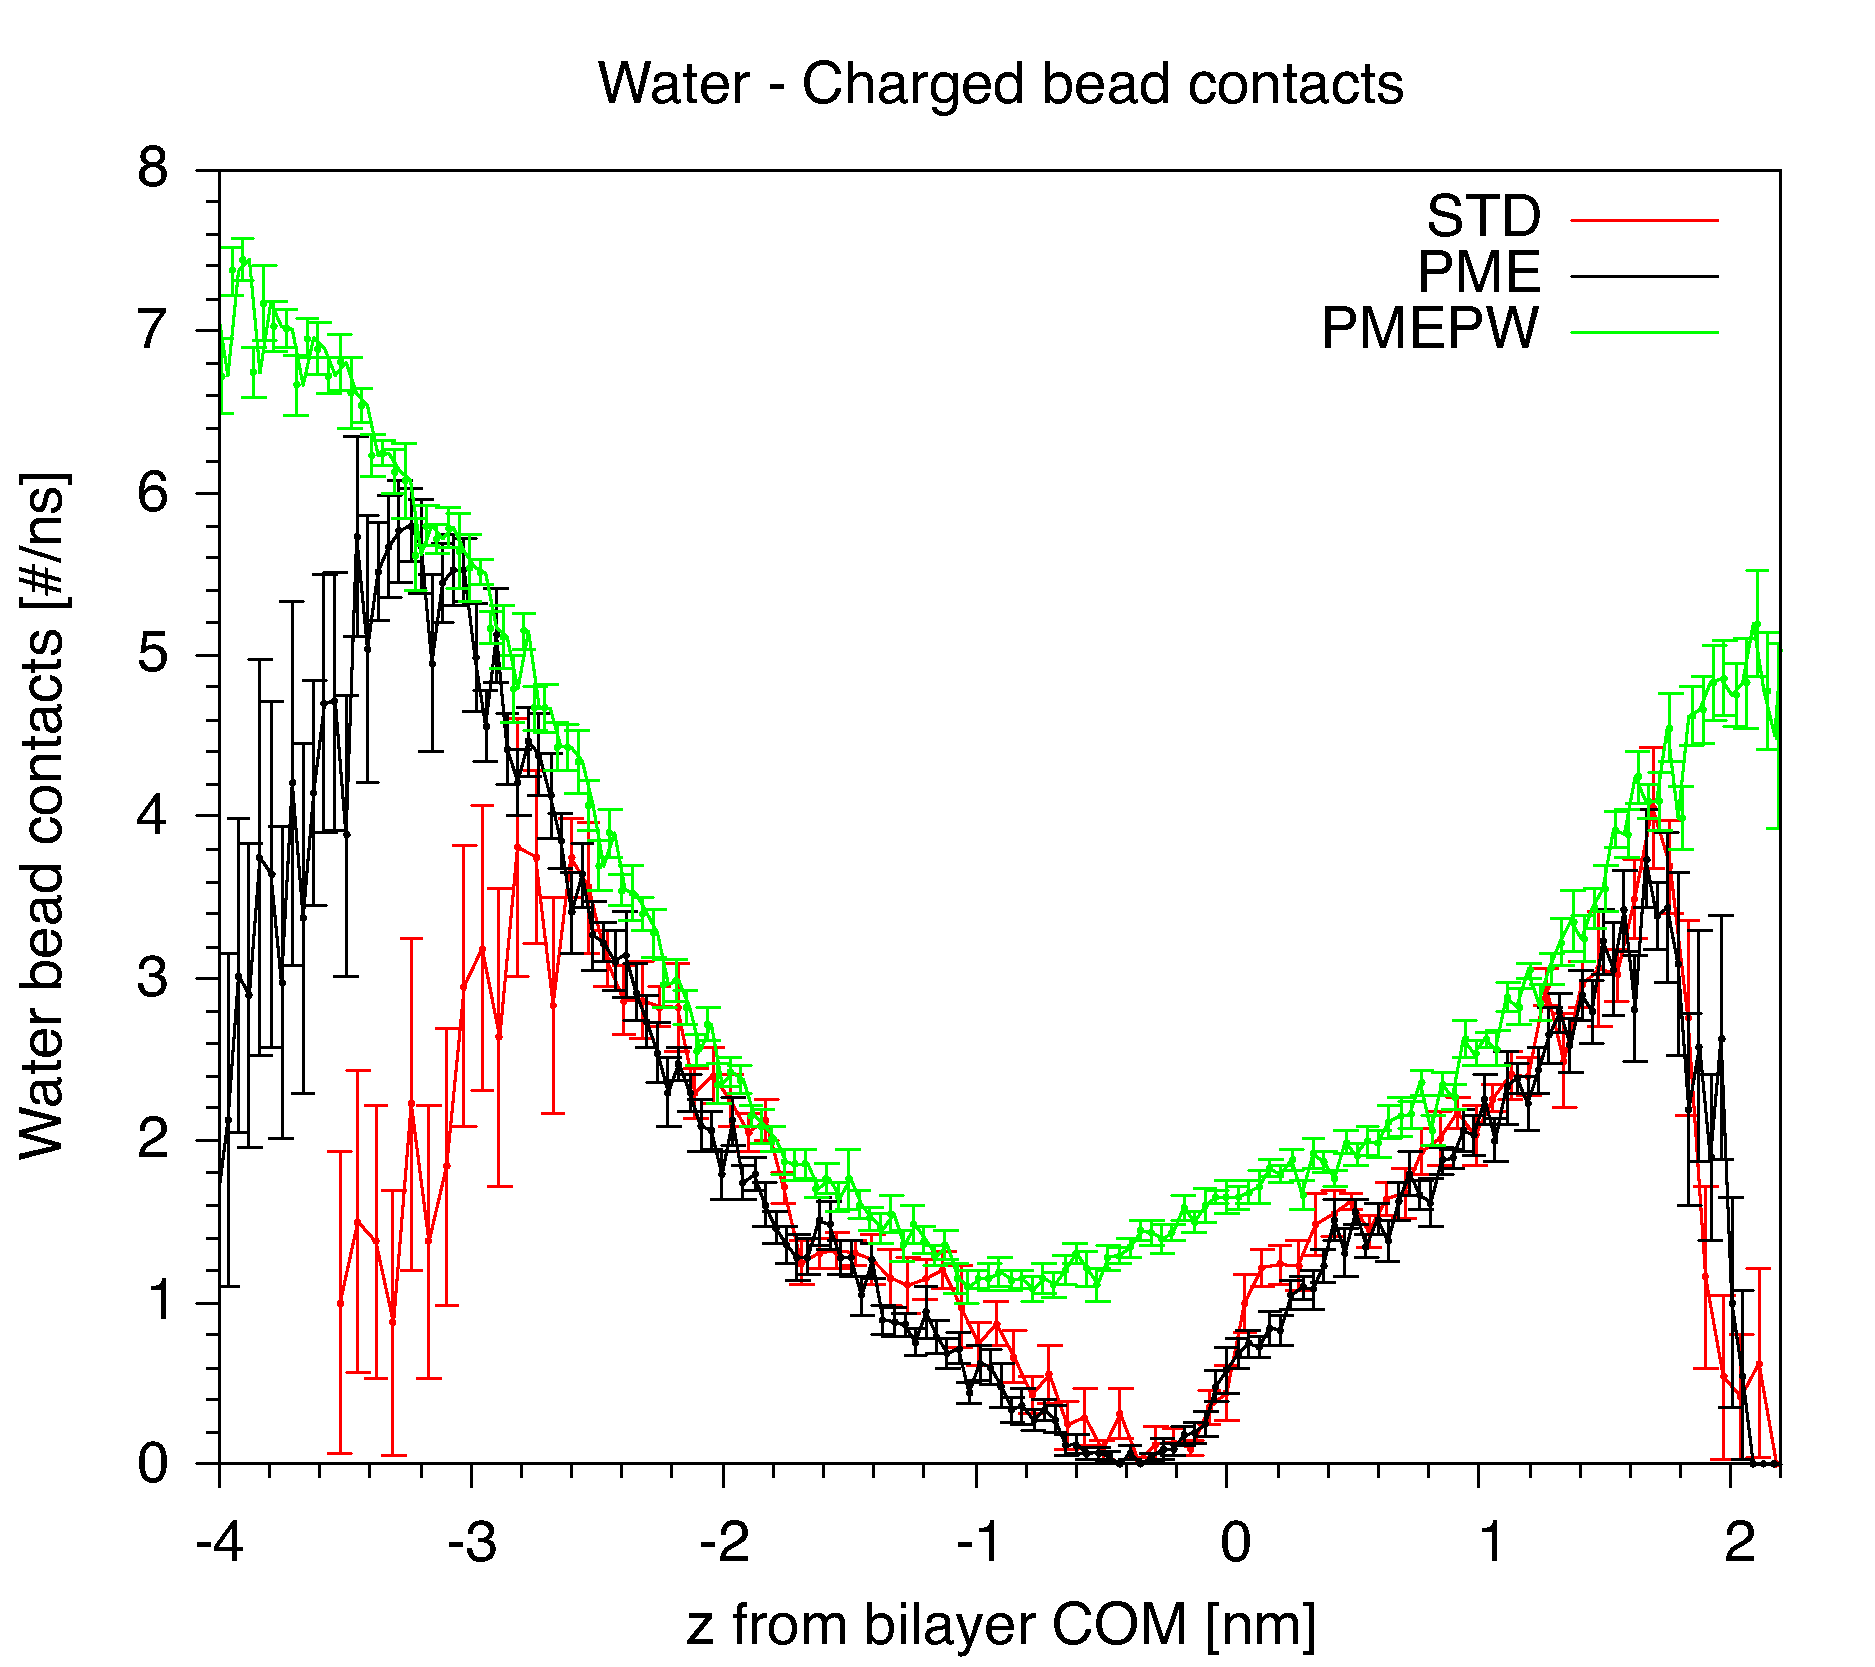
\includegraphics[width=0.5\textwidth]{./img/results/WPatchedComparison}
	}%
	\subfloat[Random and striped NP comparison]{
		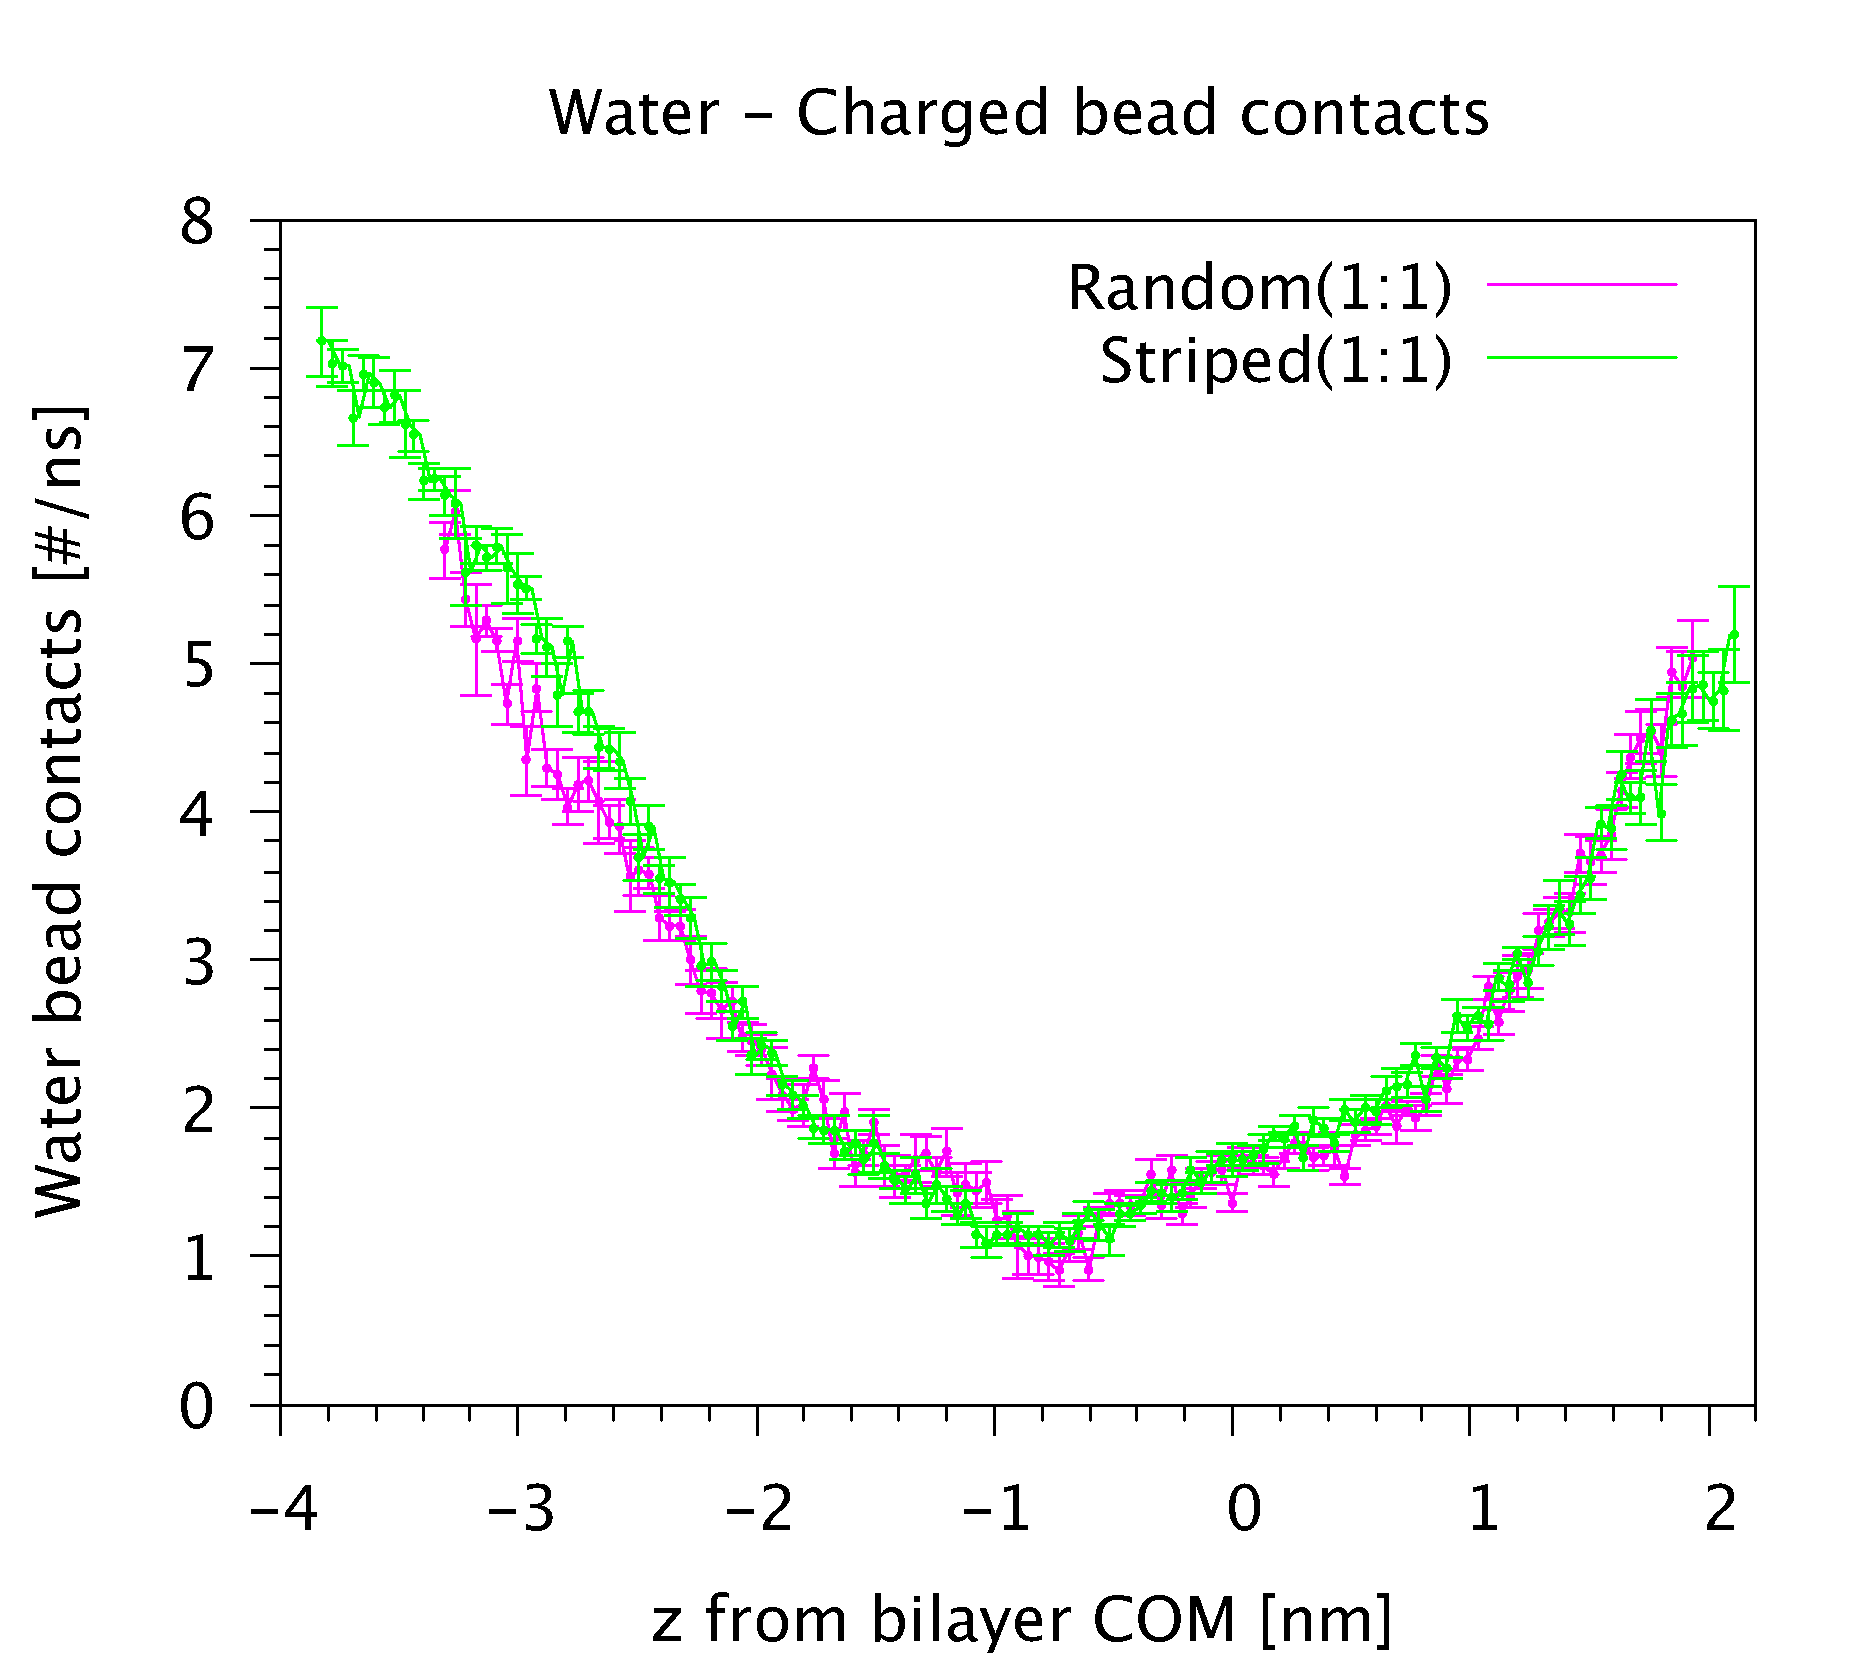
\includegraphics[width=0.5\textwidth]{./img/results/WRPComparison}
	}\\%
	\subfloat[Striped NP: atomistic model]{
		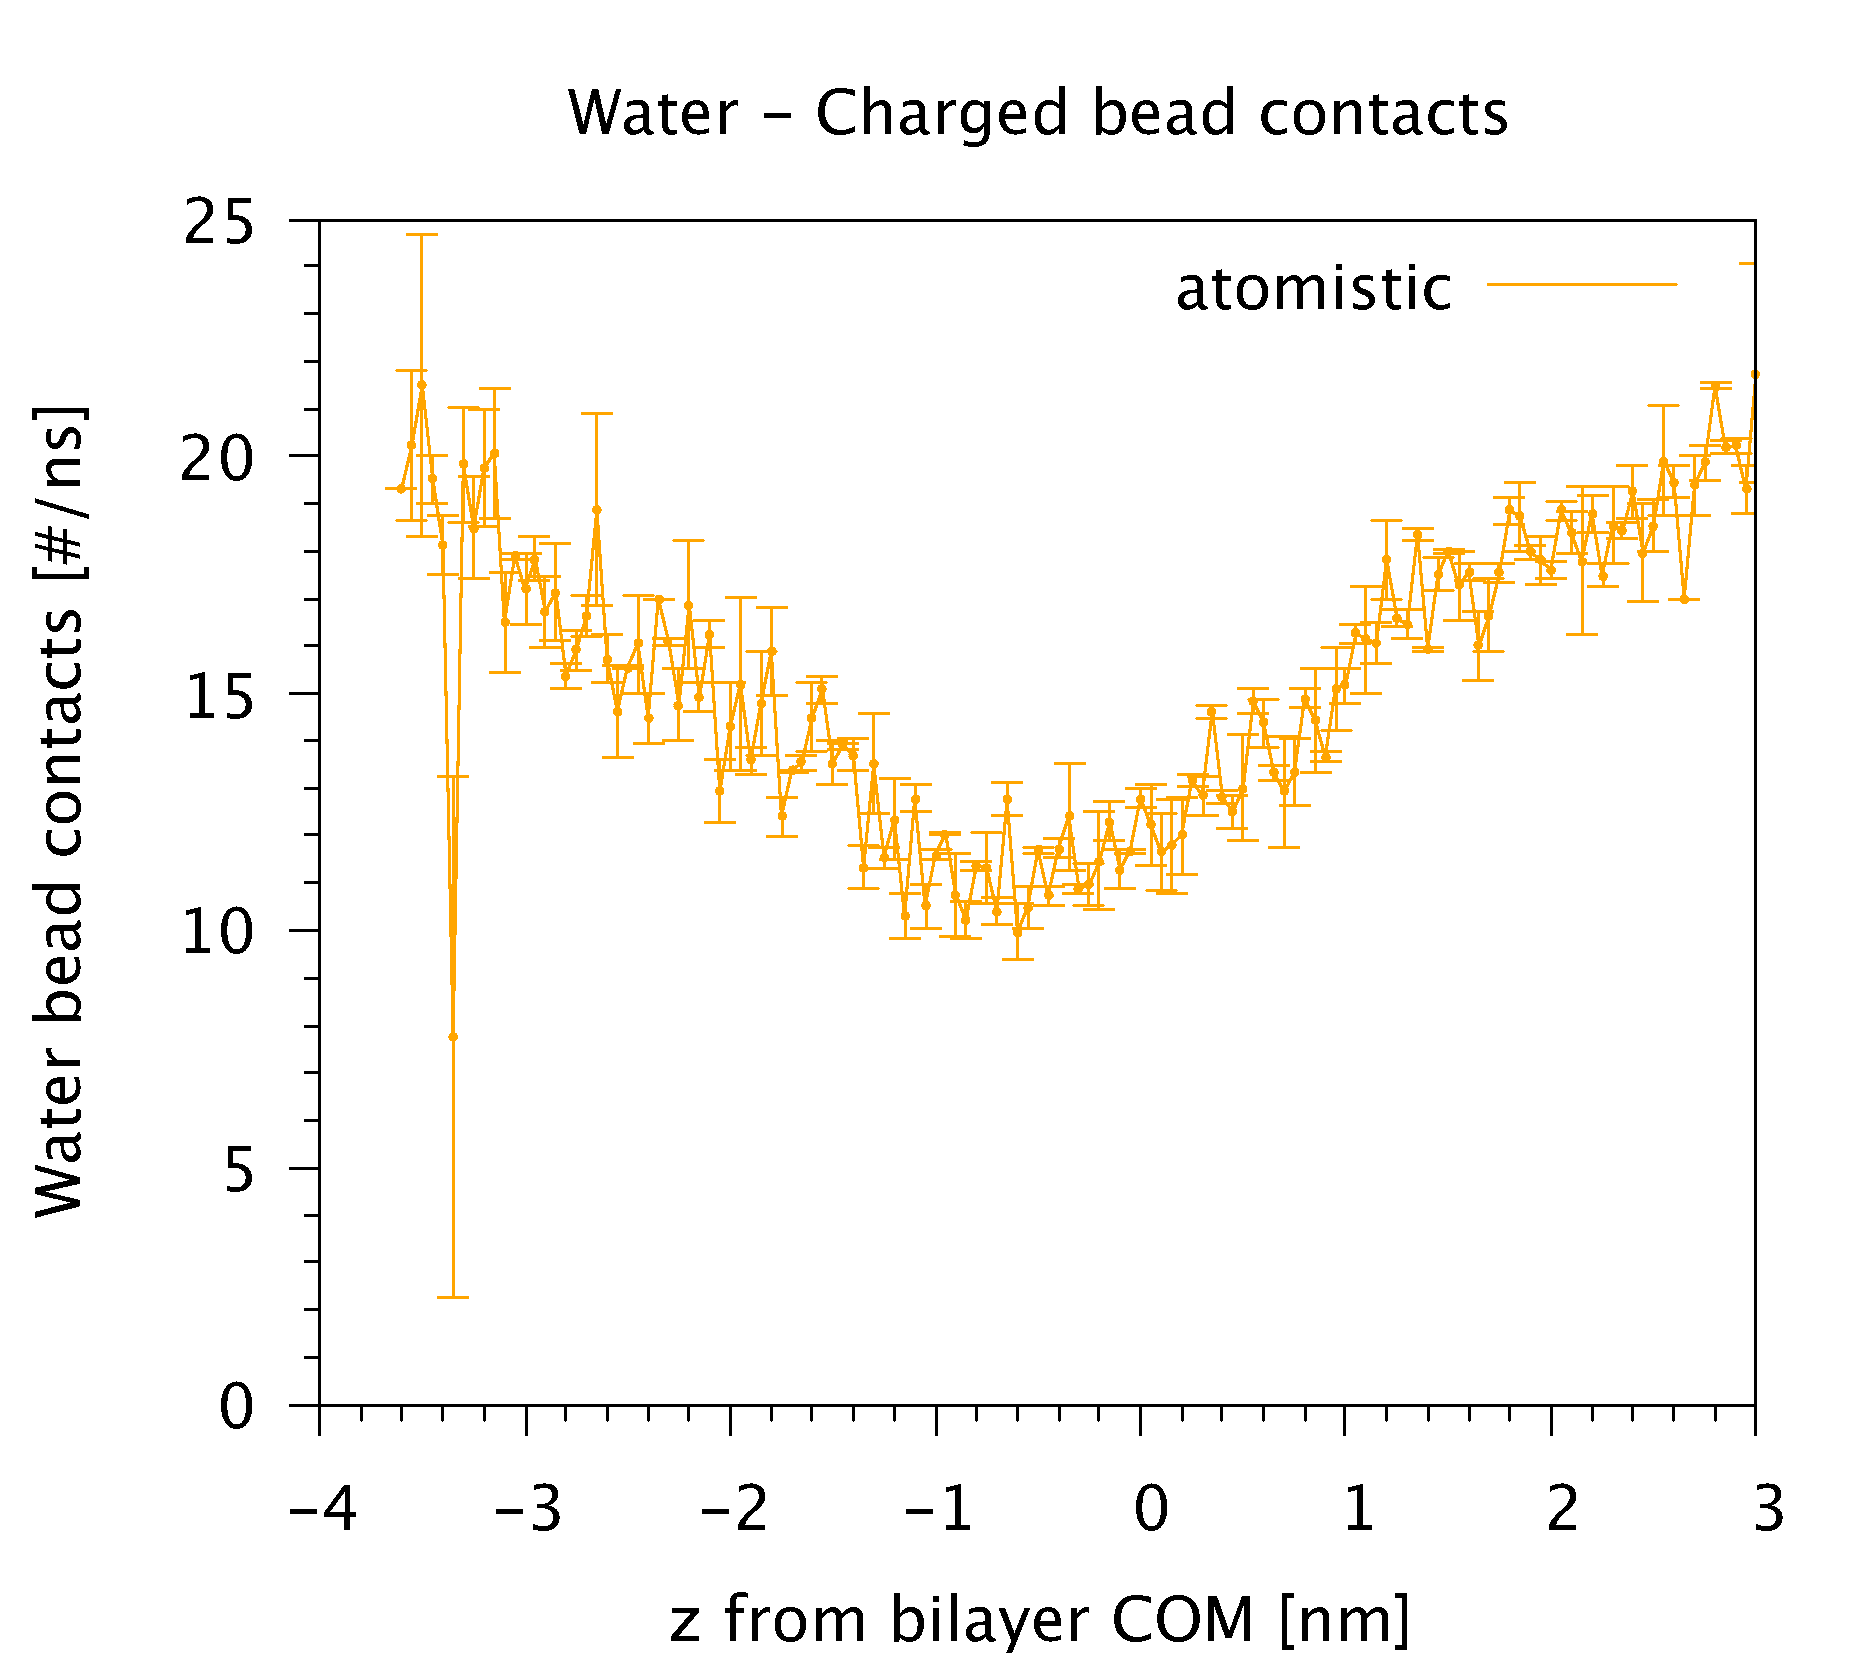
\includegraphics[width=0.5\textwidth]{./img/results/WPatchedAtomistic}
	}%
	\caption{Number of contacts per ns between water beads and the charged ligand terminal subject to the metadynamics bias potential in function of the position of the charged ligand terminal. For $z<0$ the charged ligand terminal is near the entrance leaflet. (a) For the striped \acs{NP} with different models. (b) For the striped and the random \acs{NP}s with \acs{PME}+\acs{PW}. (c) For the striped \acs{NP} with the atomistic model (data courtesy of F. Simonelli). The \ac{CG} data are binned with a bin width of $0.08$~nm while the atomistic with a bin width of $0.05$~nm. For each histogram, the total number of counts per bin is normalized with the number of the bin entries. The error bar is the standard error of the mean value.}%
	\label{fig:WContact}
\end{figure}

As we can see from figure~(\ref{fig:WContact}a) for the \ac{STD} \martini{} model and for the model with \ac{PME} 
alone we observe that the number of water contacts drops to zero in the core of the hydrophobic region. For the 
model with the \ac{PME}+\ac{PW} there is at least one contact per ns even in the core of the bilayer. This does 
not necessary mean that some \ac{PW} beads eventually cross the bilayer. Instead, they are bound to choline groups 
and to the charged ligand terminal. When the ligand tend to approach the core of the bilayer, or when it try to 
dis--anchor from the opposite leaflet, occurs a small deformation of the leaflet it self, as we better see from 
figures~(\ref{fig:NC3Dragging}b) and~(\ref{fig:engulfmentFrame}f), thus some water can penetrate inside the hollow 
following the choline groups and the charged ligand terminal, see figure~(\ref{fig:PWDragging}e). Also we have to 
remark that the time spent by the charged bead in the hydrophobic region is no more than $1$ or $2$~ns. The same 
behavior with the \ac{PW} model is observed also for the random \ac{NP}, shown in figure~(\ref{fig:WContact}b). In 
figure~(\ref{fig:WContact}c) it is plotted the number of water contacts as obtained from atomistic metadynamics 
runs. While crossing the membrane center, the atomistic charged ligand retains up to about $10-12$ contacts per ns 
with water molecules, that would correspond to $2.5-3$ contacts per ns with \martini{} \ac{CG} water beads. The 
results obtained with the \ac{PME}$+$\ac{PW} \ac{CG} model, while still underestimating the number of water beads 
dragged to the membrane center during translocation, are more consistent with the atomistic simulations than those 
obtained with the \ac{STD} \martini{} model.
% \begin{figure}[ht]
% 	\center
% 	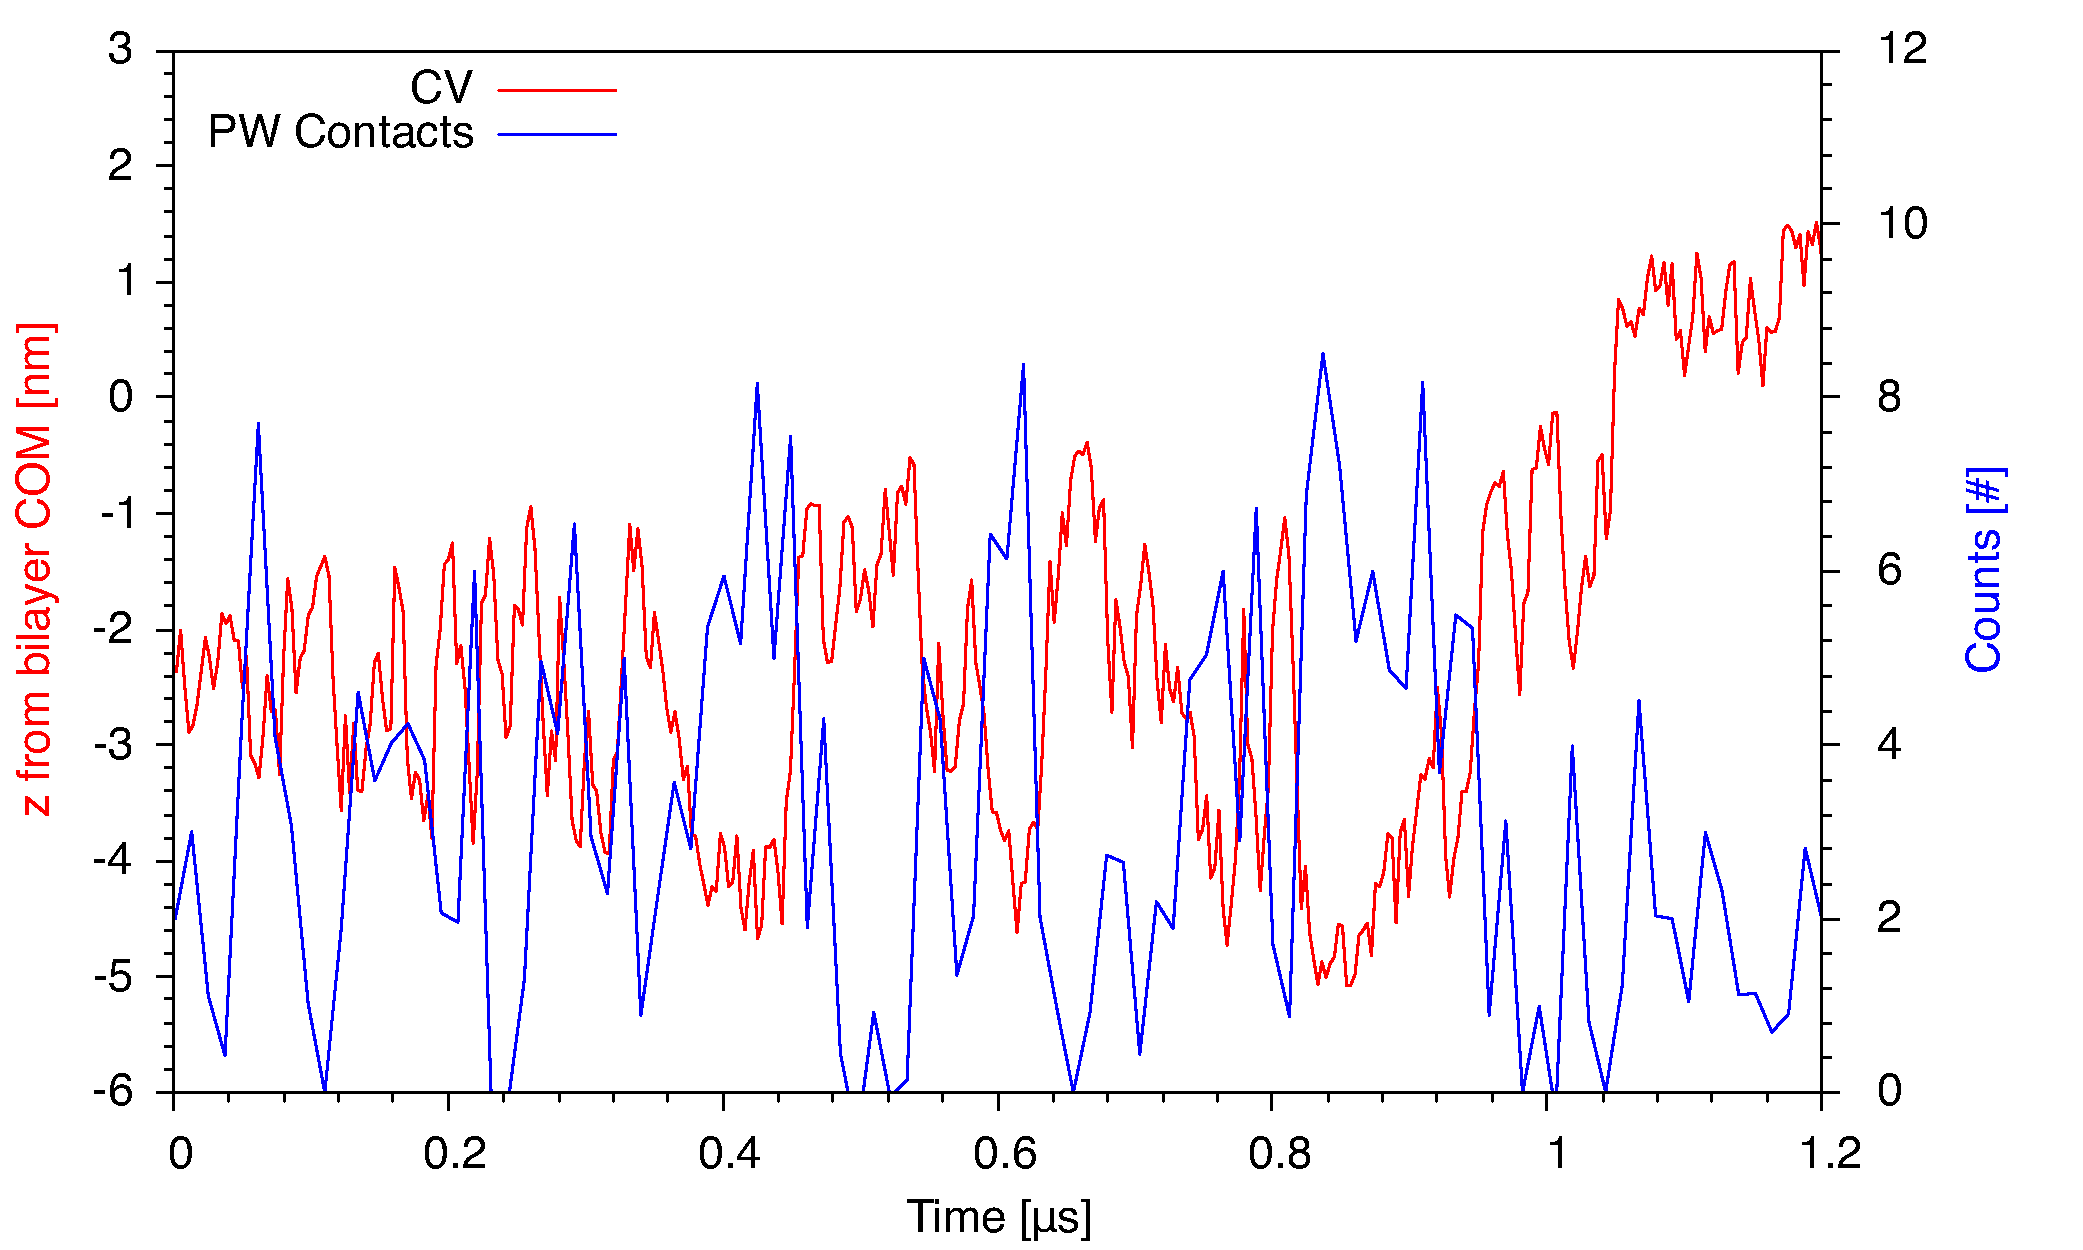
\includegraphics[width=0.9\textwidth]{./img/results/wCorrelation}
% 	\caption{Superposition of the \acs{CV} (red) and the number of contacts between the \acs{PW} beads and the charged bead (blue) in function of the time for a striped metadyamcis run. $z>0$ corresponds to the anchored state. It can be noted a clear anti--correlation between the distance of the charged bead from the bilayer \acs{COM} and the number of the \acs{PW} contacts: they decrease when the charged bead is approaching the hydrophobic region.}
% \end{figure}

\subsection{Lipid heads dragging}
%Trascinamento delle teste dei lipidi nelle varie salse
The same dragging effect of the water beads during the forward process is also noticed for the choline groups 
(NC$3$ \martini{} bead) of the lipids of the entrance leaflet. When the charged ligand terminal approaches the 
hydrophobic core of the bilayer it tends to drag the choline groups, as a result the entrance leaflet slightly 
deforms producing a small hollow. An example of this phenomenon is shown in figure~(\ref{fig:NC3Dragging}).

In order to investigate the process, in figure~(\ref{fig:NC3Correlation}) I have plotted the \ac{CV}, which is the 
distance of the charged ligand terminal from the bilayer \ac{COM} (red); and $d_\text{min}^{\text{NC}3}$, which is 
the minimum distance of the choline groups from the bilayer \ac{COM} (blue) as a function of time. We can see an 
evident correlation: when the ligand tends to approach the center of the membrane the minimum distance between the 
choline groups and the center of the membrane decreases, as well. This suggests that some choline groups are 
strongly bound to the charged ligand terminal while the latter tries to penetrate into the membrane hydrophobic 
region.
\begin{figure}[!ht]
	\center
	\subfloat[]{%
		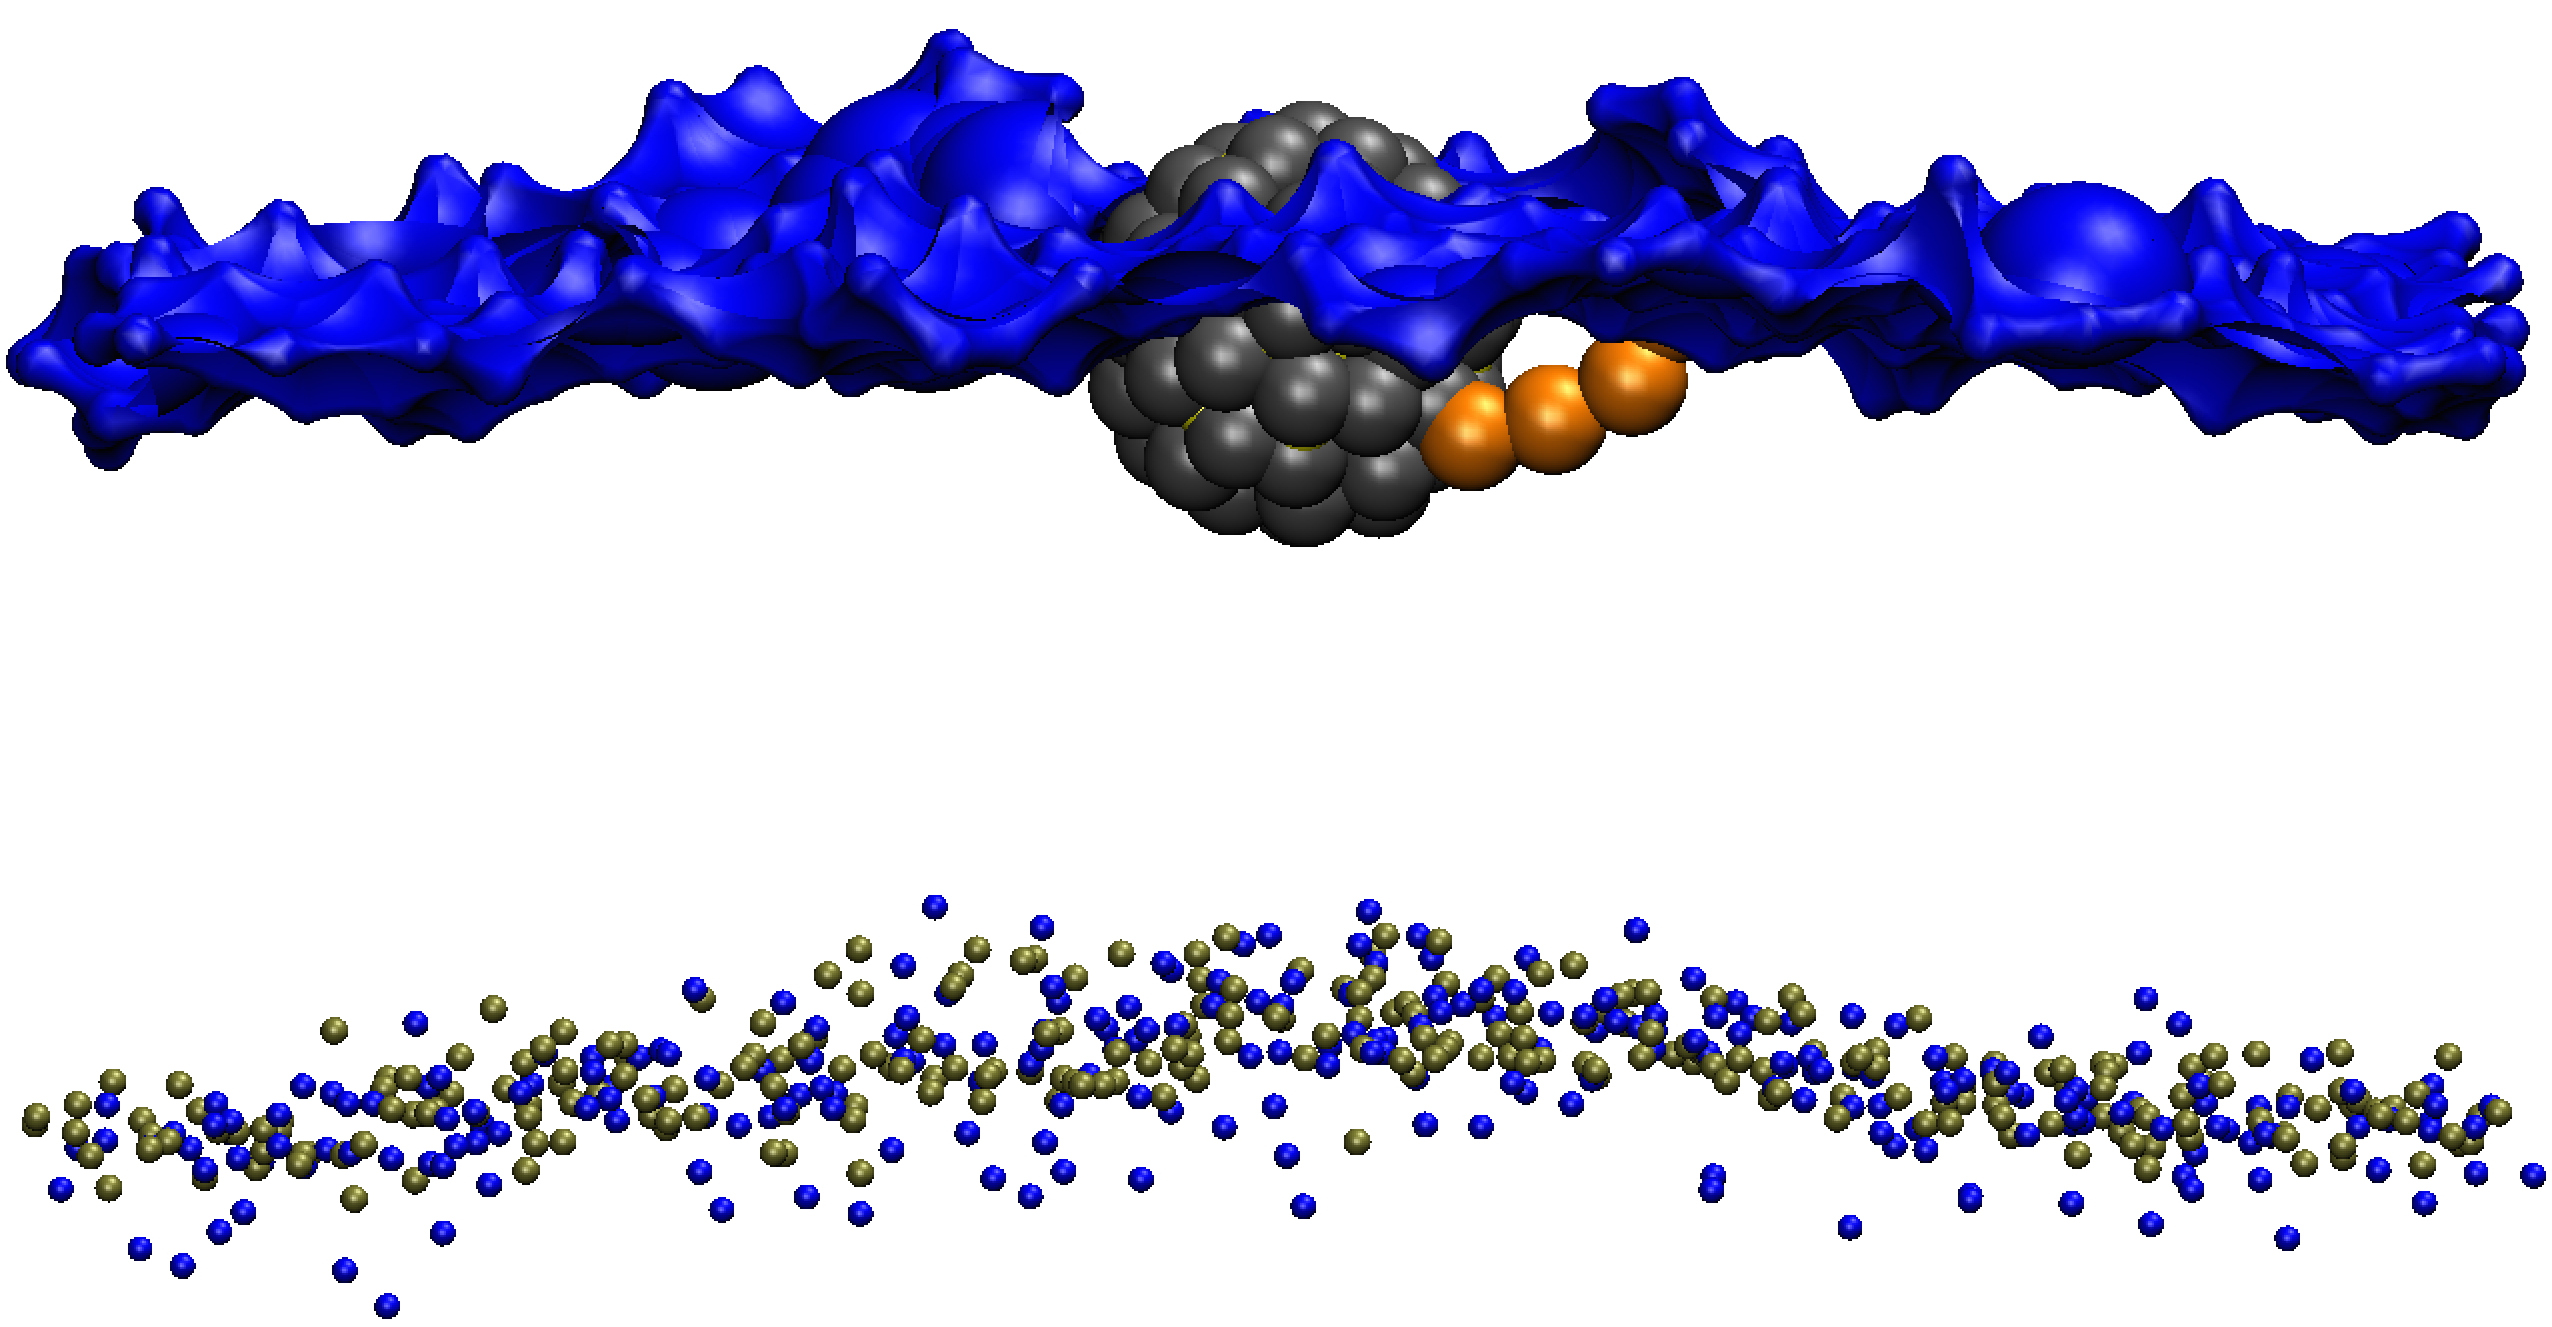
\includegraphics[width=0.47\textwidth]{./img/NC3PWFrame/NC3a.png}%
	}\ %
	\subfloat[]{%
		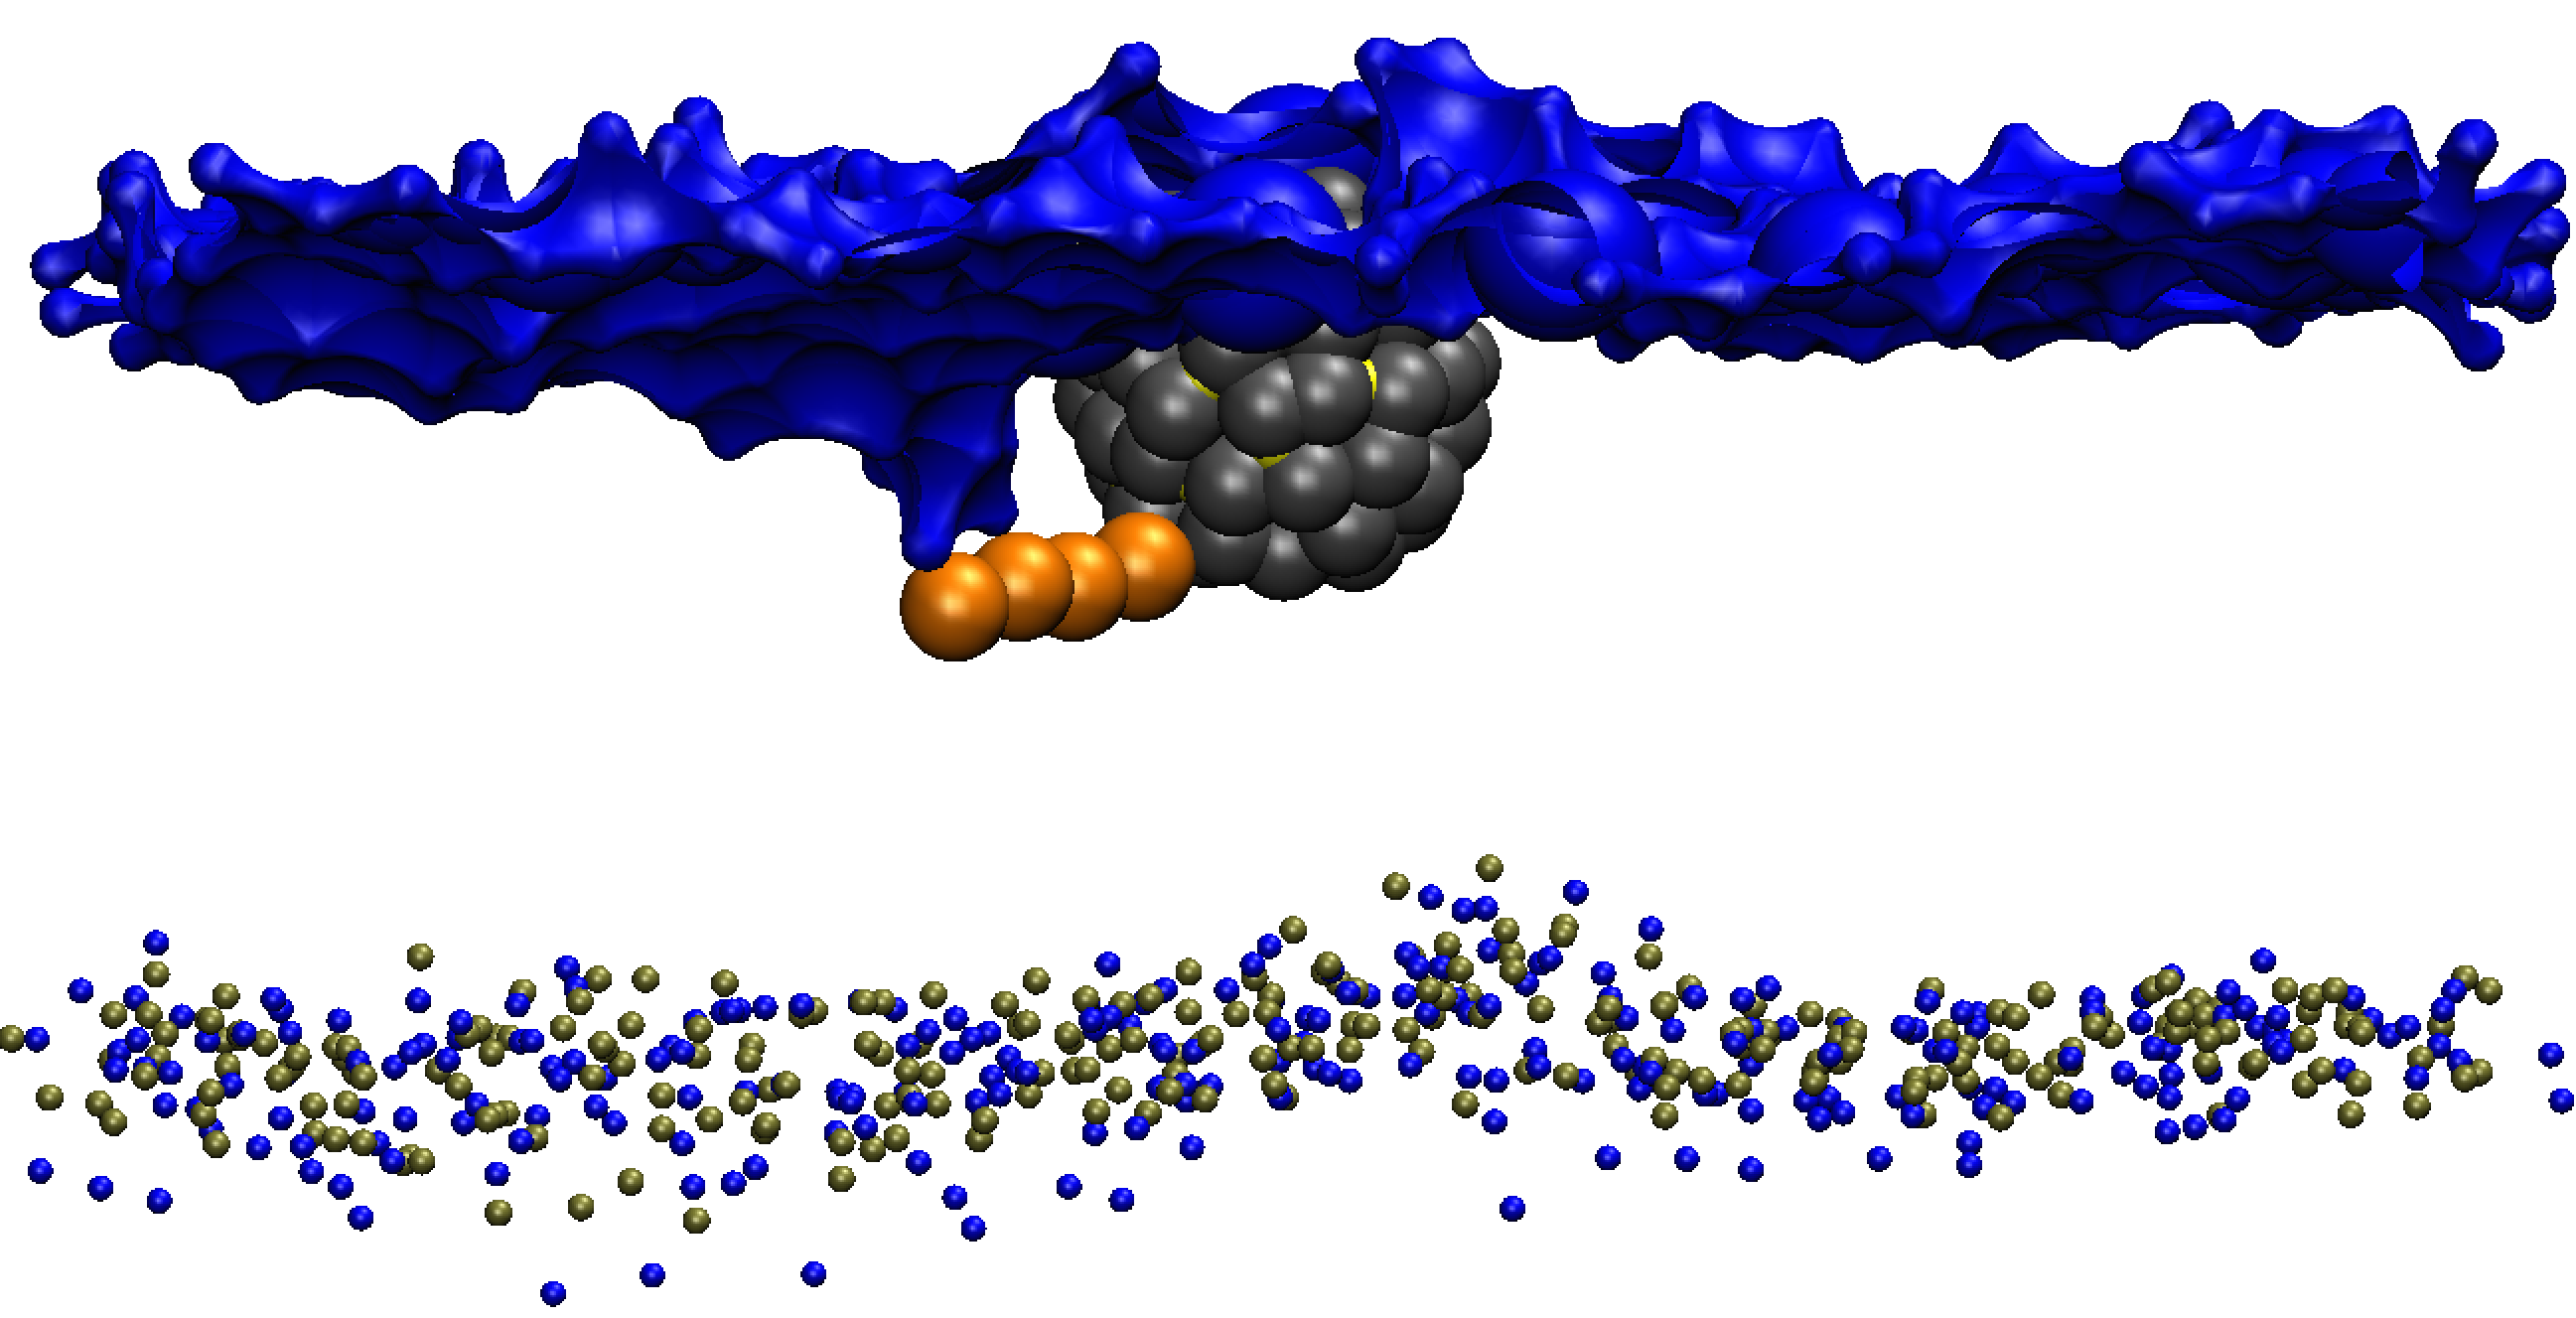
\includegraphics[width=0.47\textwidth]{./img/NC3PWFrame/NC3b.png}%
	}\\\medskip%
	\subfloat[]{%
		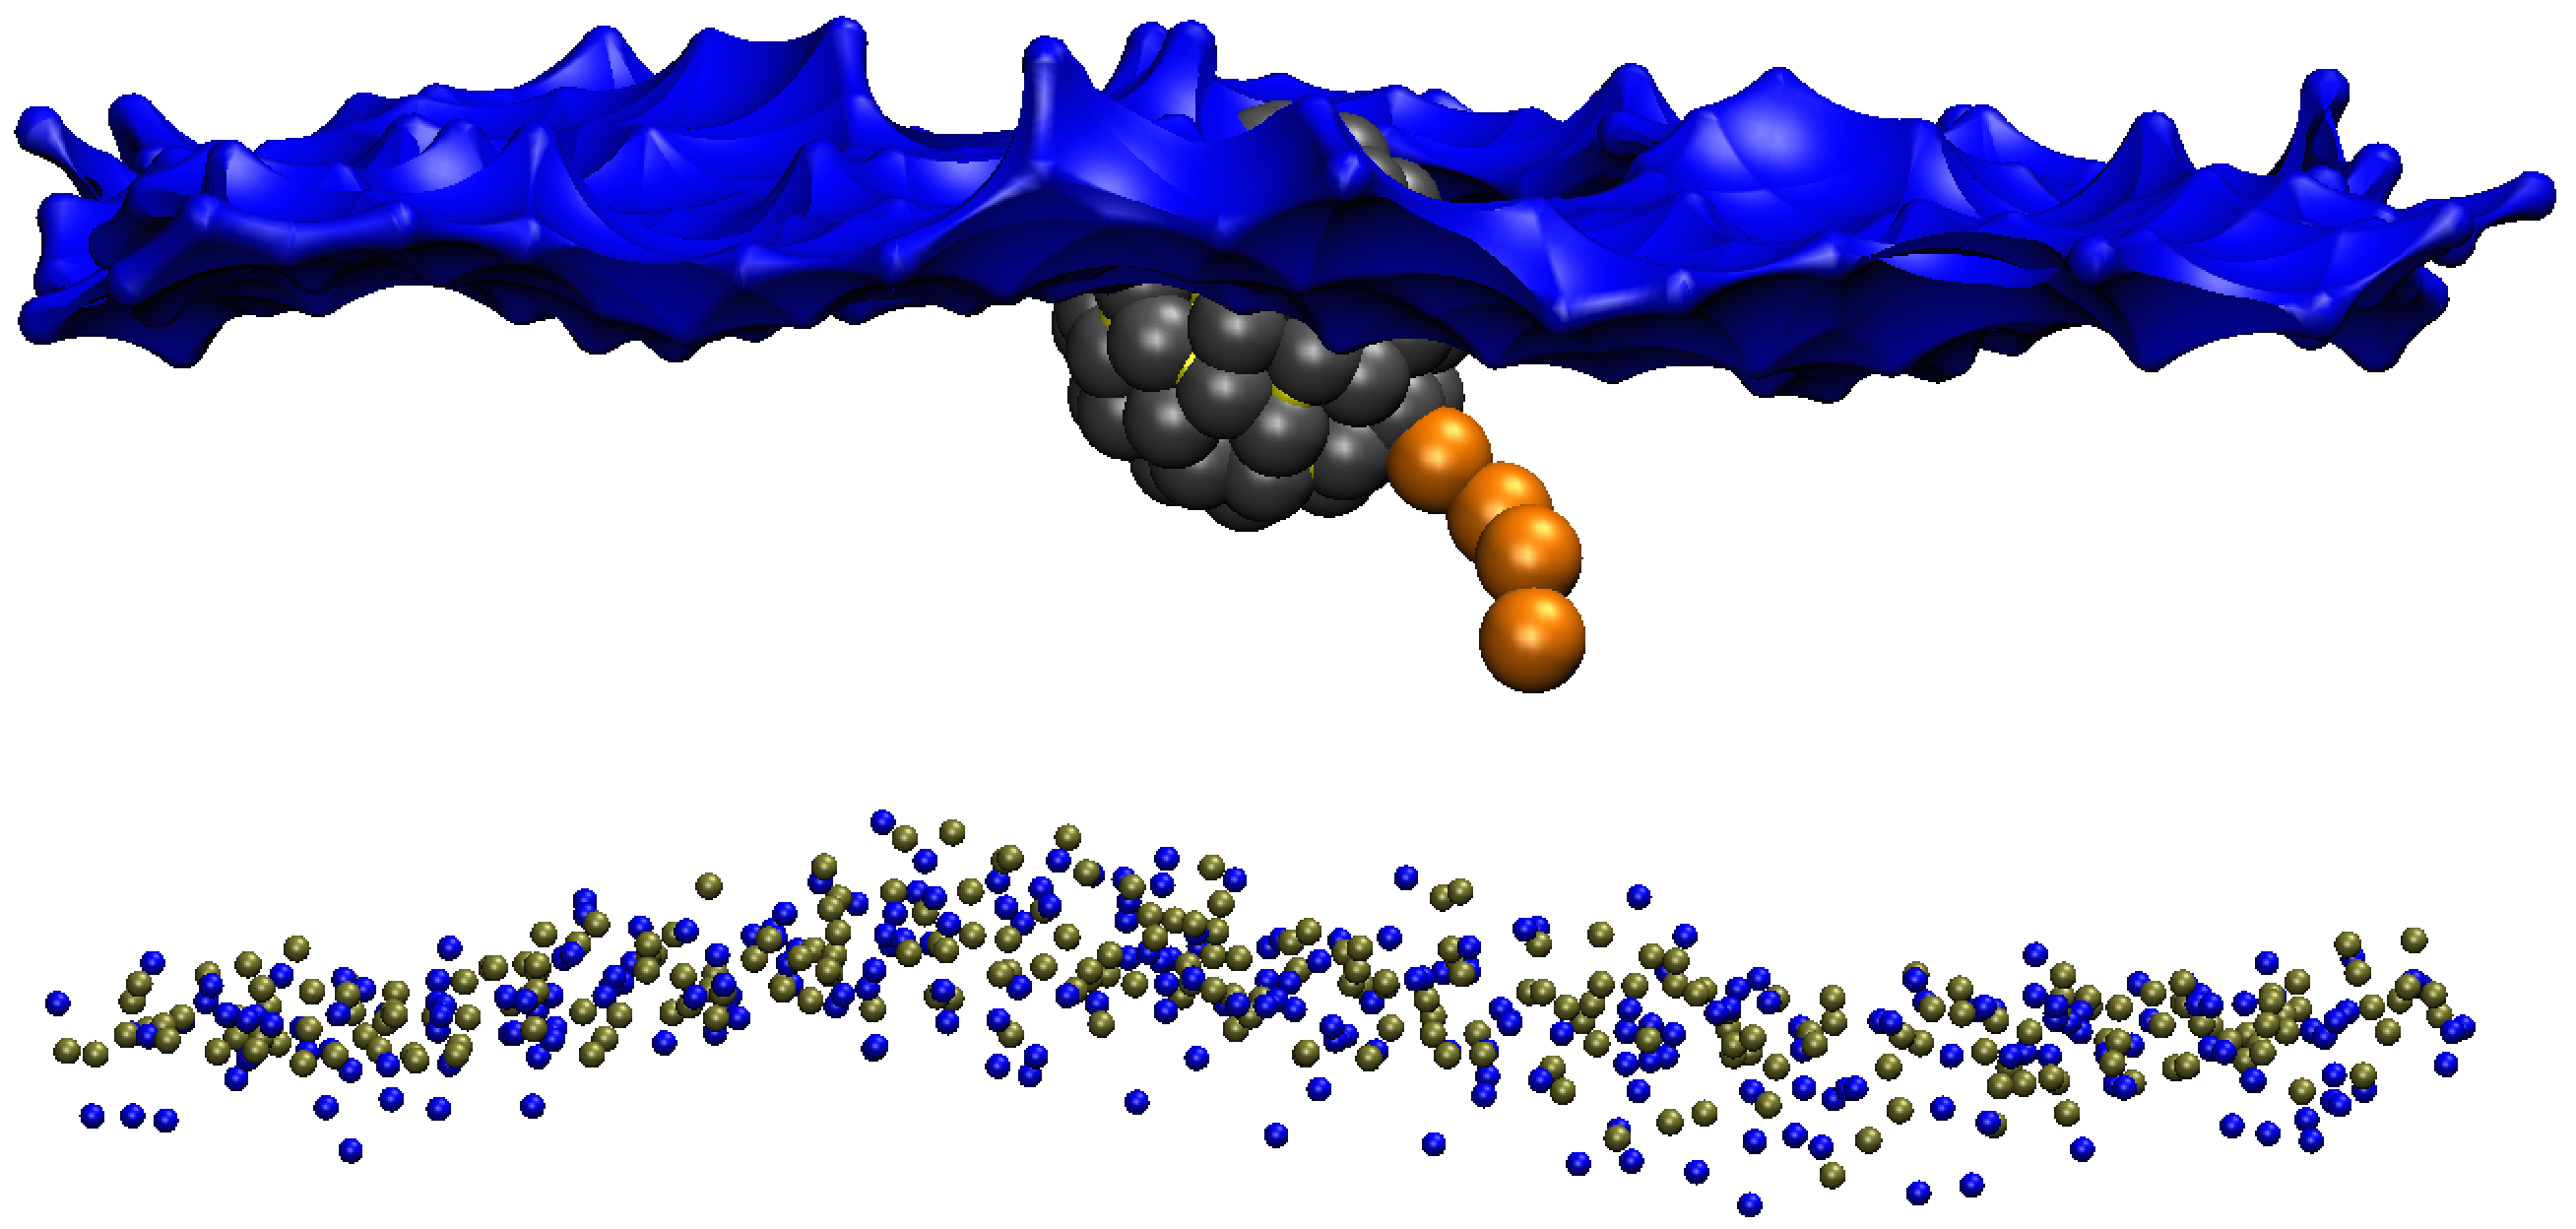
\includegraphics[width=0.47\textwidth]{./img/NC3PWFrame/NC3c.png}%
	}%
	\caption{Same frames of figure~(\ref{fig:metaFrame}a-c), respectively. In (a) the normal configuration of the lipid heads in the entrance leaflet during the hydrophobic state. In (b) an example of the dragging effect of the lipid heads inside the center of the bilayer by the charged ligand and in (c) no deformation occur since the changed ligand is no more bound to the lipid heads of the entrance leaflet. Color code as in figure~(\ref{fig:threeProcess}). The surface in blue is the surface representation of the choline and phosphate groups. The charged ligand chosen for the metadynamics is in orange. Water beads, lipid tails and the other \acs{NP} ligands are not shown.}%
	\label{fig:NC3Dragging}
\end{figure}
\begin{figure}[!ht]
	\center
	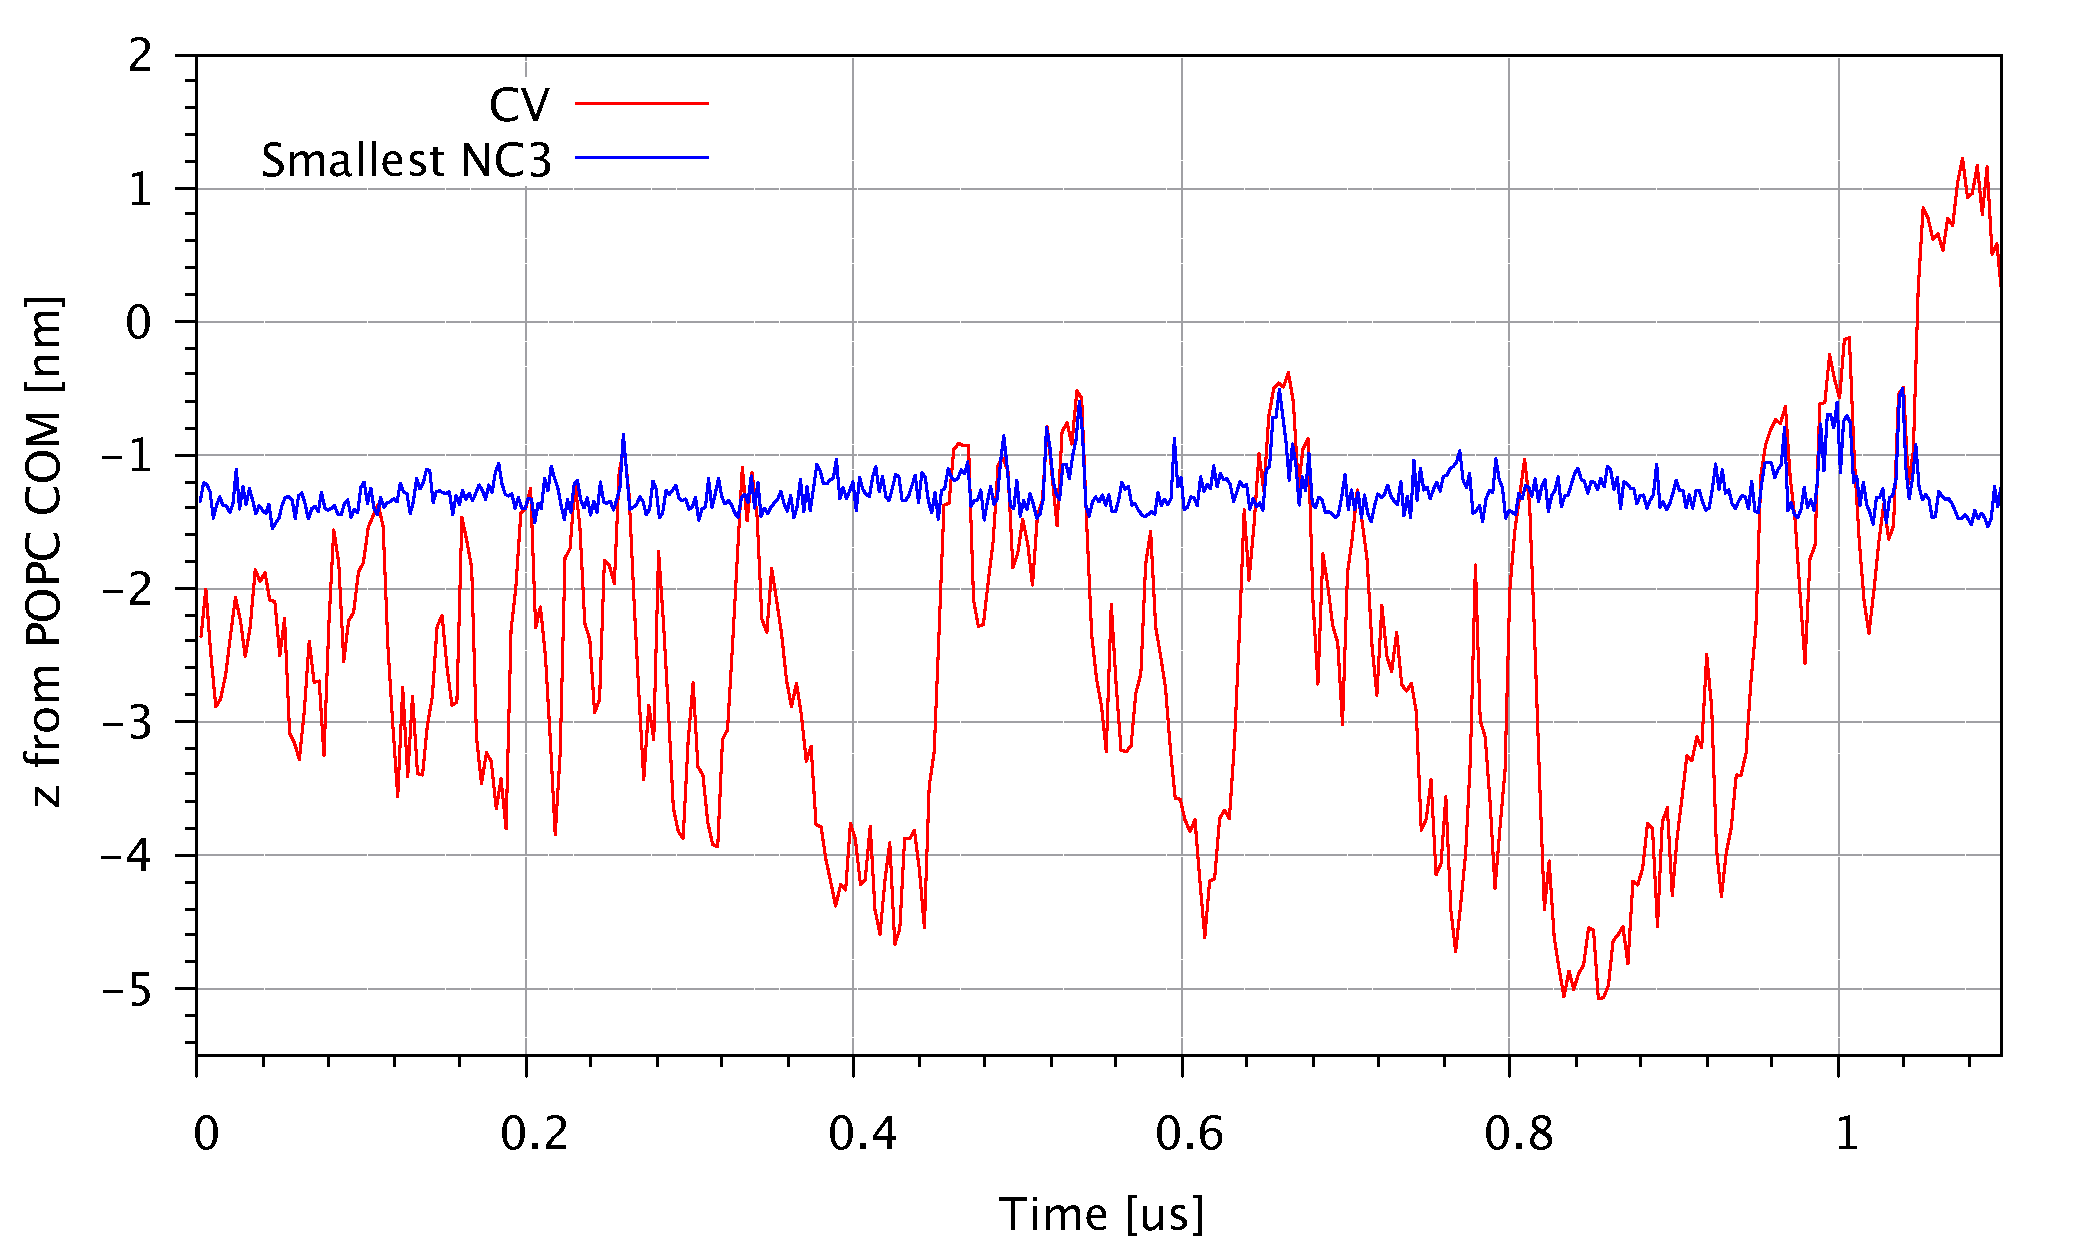
\includegraphics[width=0.8\textwidth]{./img/results/NC3Correlation}
	\caption{Superposition of the \acs{CV} (red) and $d_\text{min}^{\text{NC}3}$, the minimum distance, along $z$, between the choline groups of the lipid of the \acs{NP} entrance leaflet and the bilayer \acs{COM} (blue) as a function of time. The data are from a metadynamics run of a striped \acs{NP} with \acs{PME}+\acs{PW}. $z>0.5$~nm corresponds to the anchored state. In order to reduce the noise, both the \ac{CV} and the choline  distances data are filtered with a rolling mean filter: the former over four points, the latter over two points.}%
	\label{fig:NC3Correlation}
\end{figure}
Since the flip-flopping energy for a \ac{POPC} lipid is too high, when the charged bead is too far from the entrance leaflet the choline groups detaches and goes back to the entrance leaflet.

To better investigate such process, in figure~(\ref{fig:NC3minDist}) I show an histogram of the distribution of 
$d_\text{min}^{\text{NC}3}$ in the entrance leaflet. The distribution of the choline groups in the \ac{NP} 
entrance leaflet are compared to that obtained from a reference pure \ac{POPC} membrane. All the data are from 
runs with both \ac{PME} and \ac{PW} and were obtained via both biased and unbiased \ac{MD} simulations. In both 
the metadynamics and unbiased \ac{MD} runs, i.e. when the \ac{NP} is present, we can observe that the distribution 
of the lipid heads shifts towards the membrane center.
% 	minDistPatched			minDistRandom11
\begin{figure}[th!]
	\center
	\subfloat[Striped NP]{
		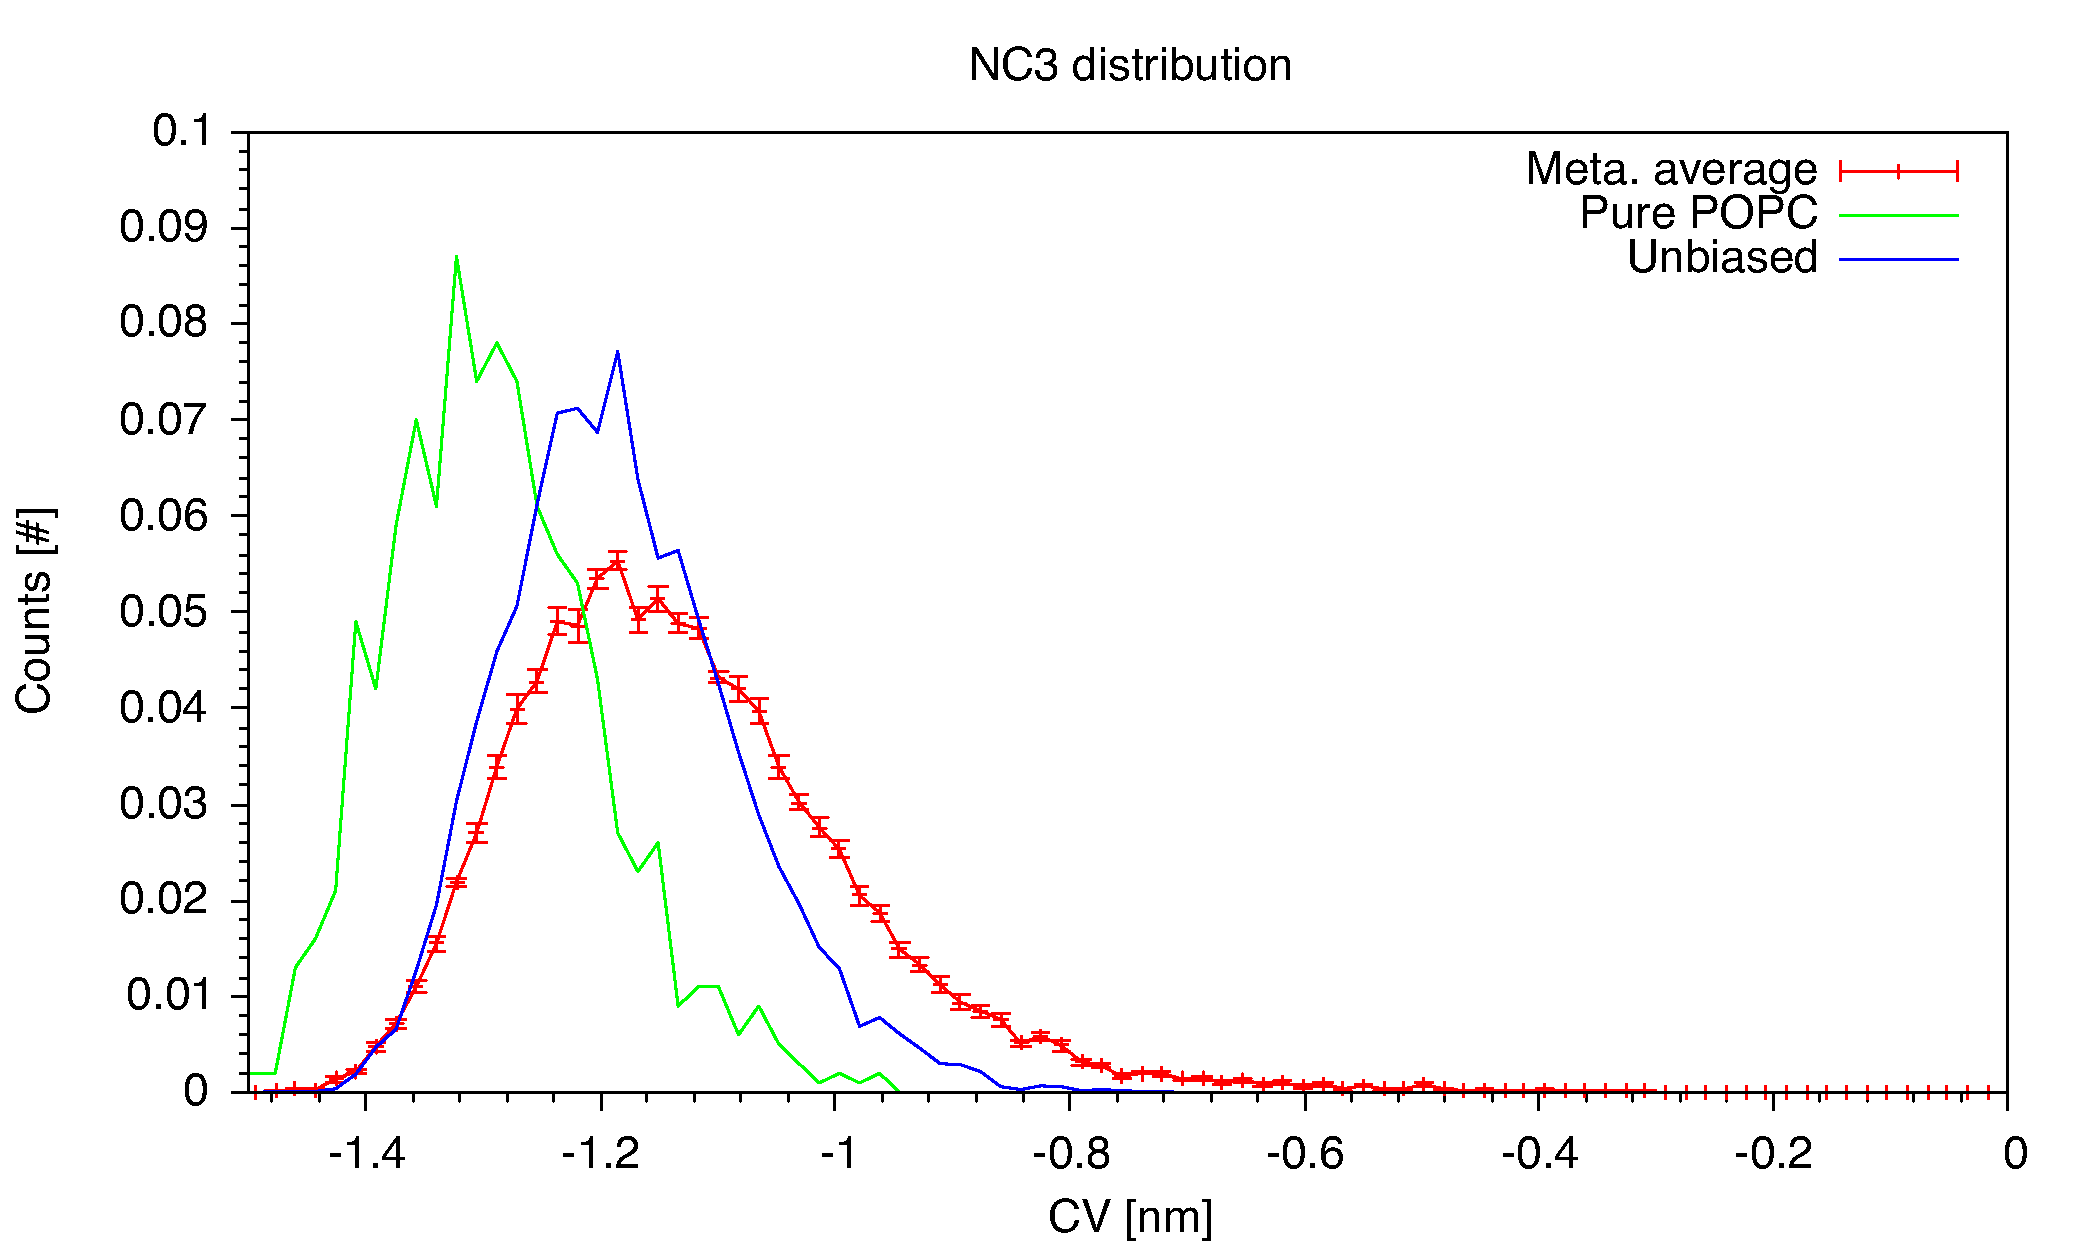
\includegraphics[width=0.85\textwidth]{./img/results/minDistPatched}
	}\\%
	\subfloat[Random NP]{
		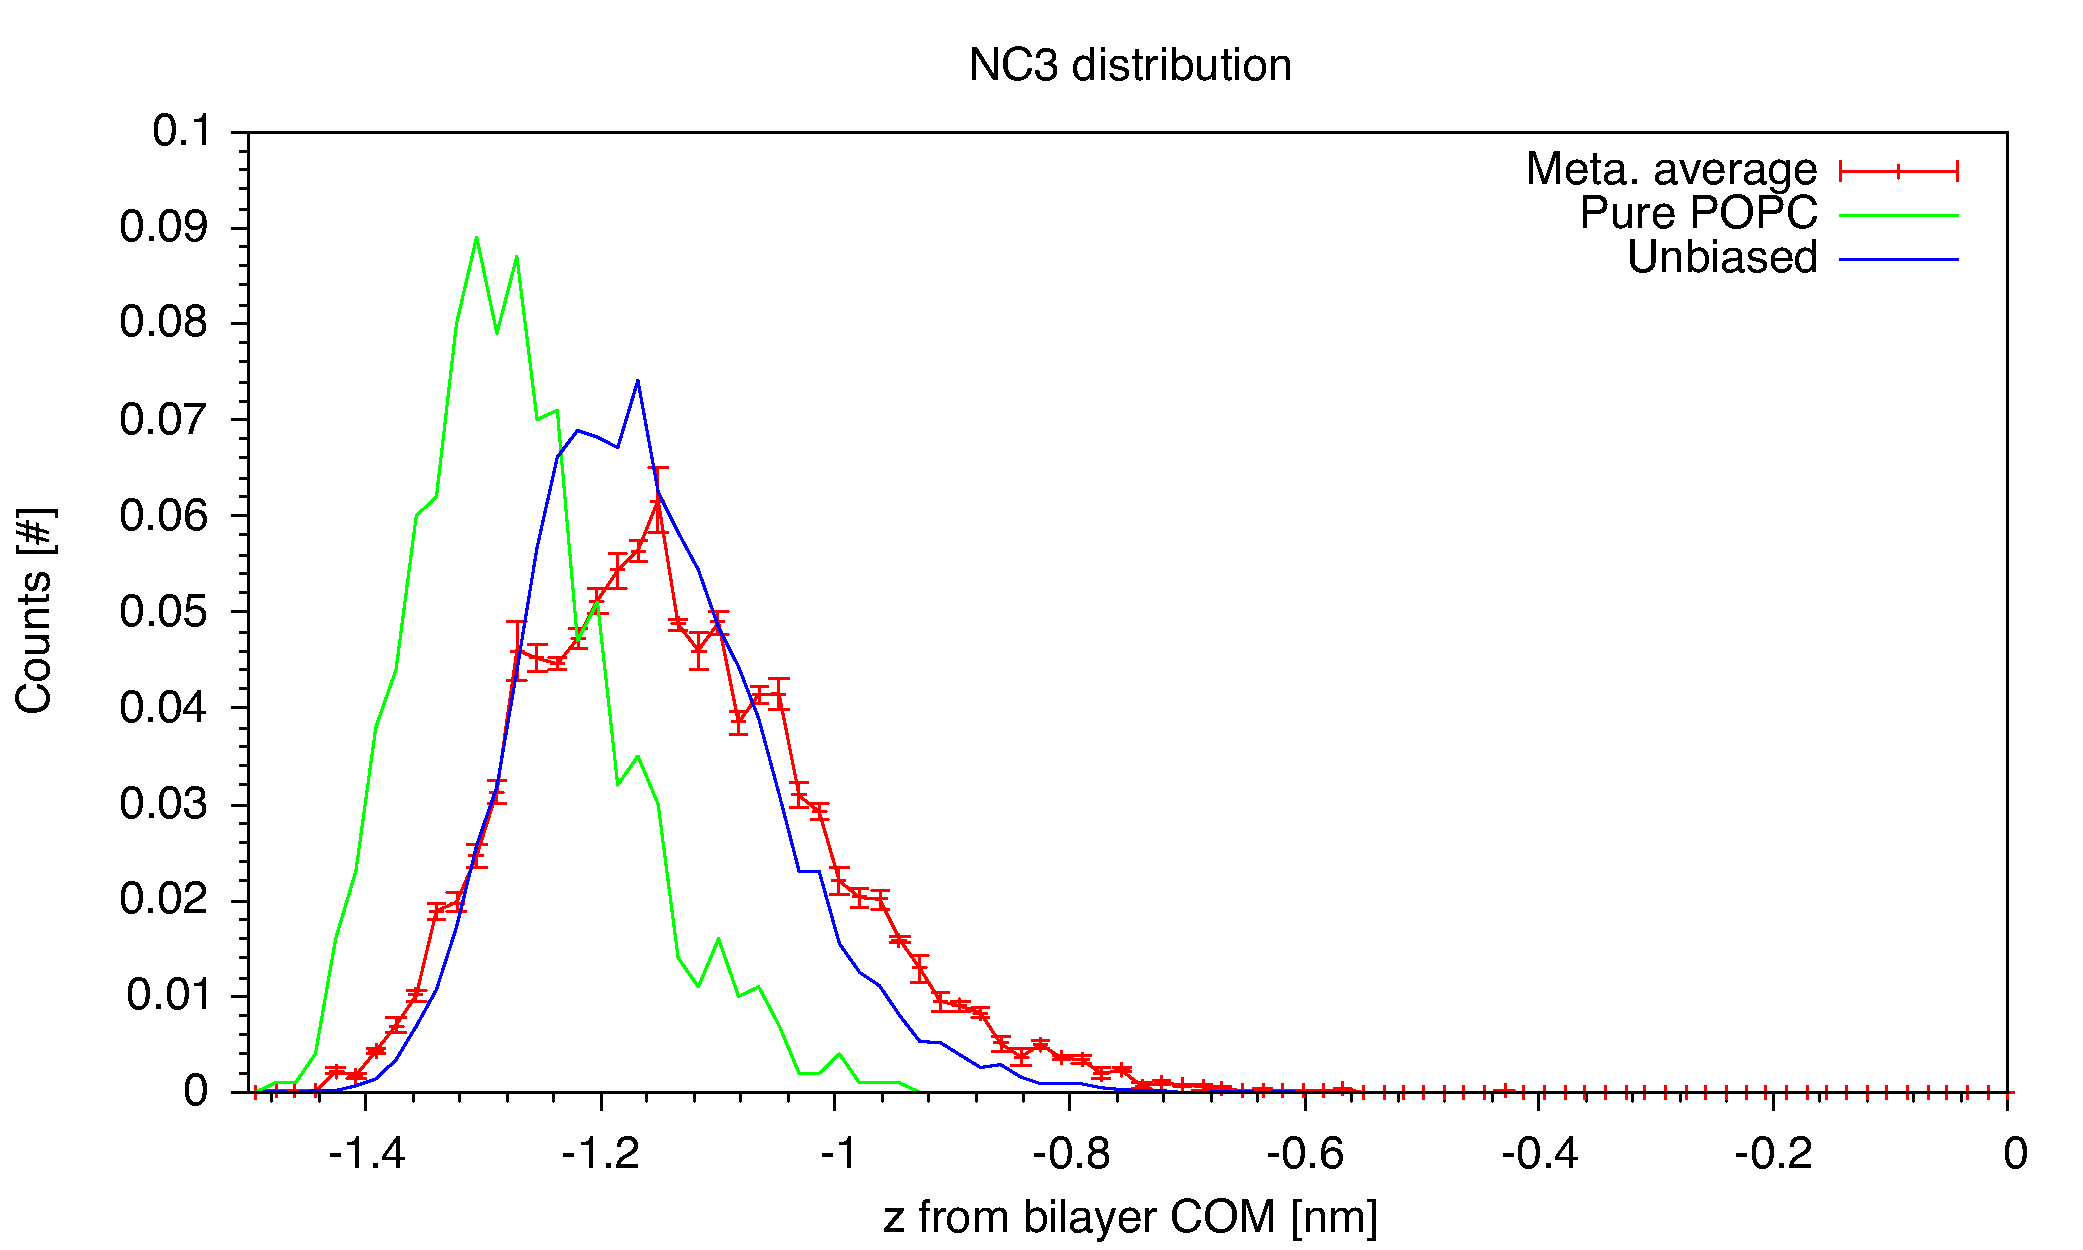
\includegraphics[width=0.85\textwidth]{./img/results/minDistRandom11}
	}%
	\caption{Distribution of $d_\text{min}^{\text{NC}3}$ in the entrance leaflet. The red curve is from an average over the metadynamics runs considering the whole trajectory. The blue curve is from the unbiased run and the green one is from a pure \acs{POPC} membrane. (a) For the striped \acs{NP}. (b) For the random \acs{NP}. The bin width is $0.02$~nm for all curves and each histogram is normalized to the total number of entries. The error bar for the metadynamics runs is calculated as the standard error of the mean value.}%
	\label{fig:NC3minDist}
\end{figure}

%	NC3PatchedComparison	NC3RPComparison
\begin{figure}[th!]
	\center
	\subfloat[Striped – model comparison]{
		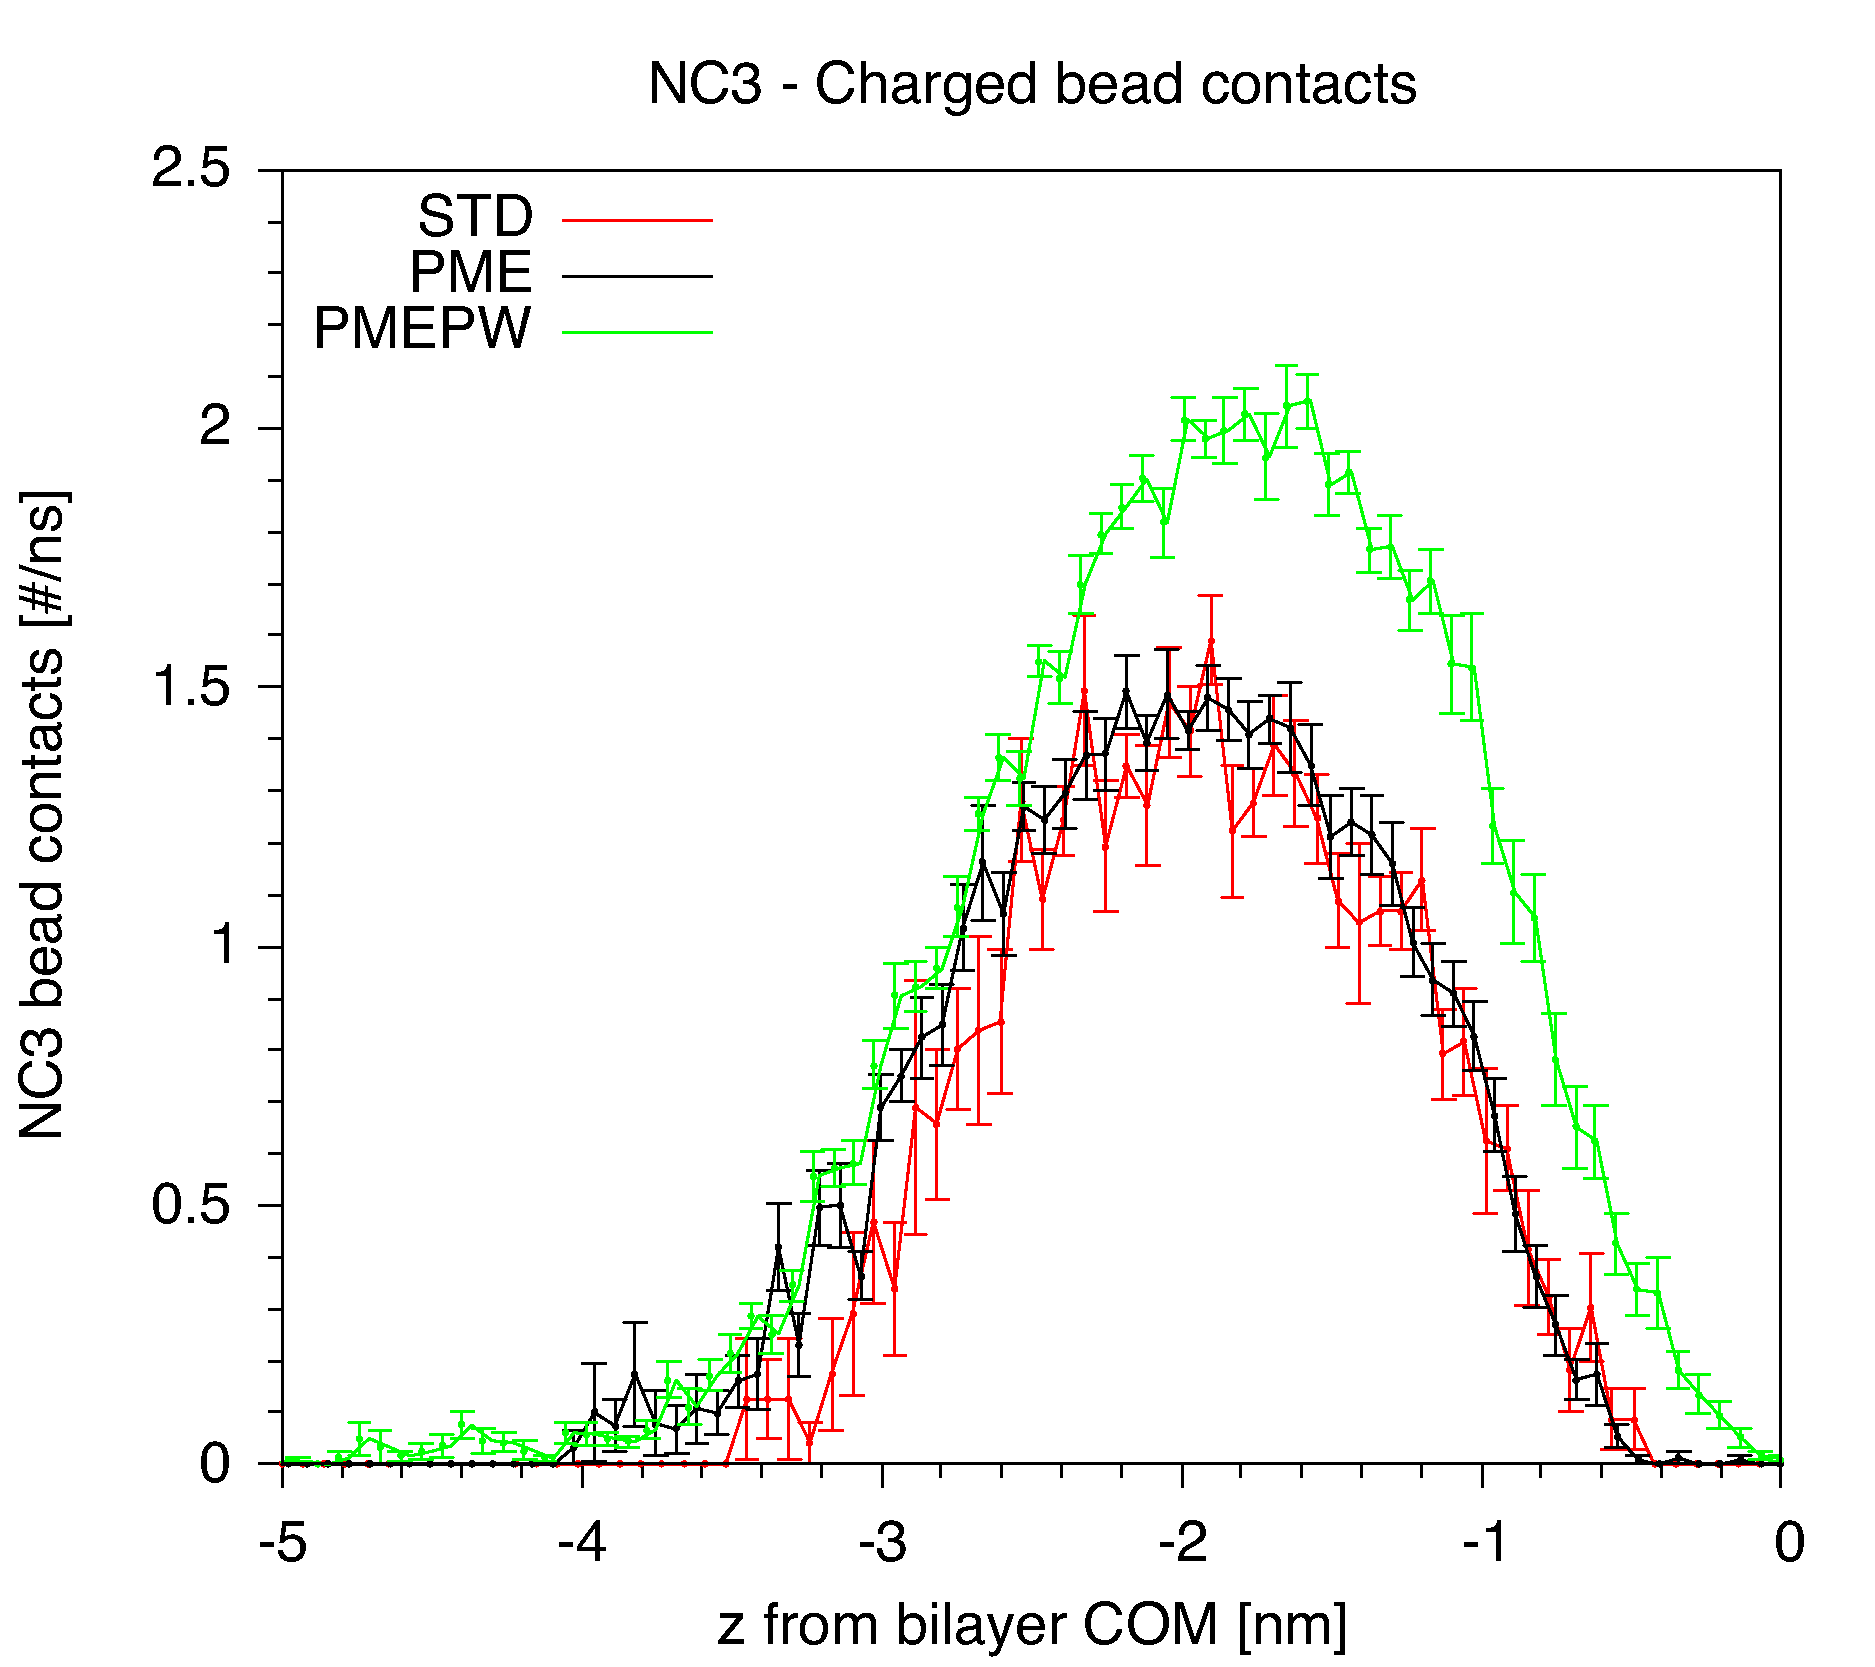
\includegraphics[width=0.5\textwidth]{./img/results/NC3PatchedComparison}
	}%
	\subfloat[Striped – random comparison]{
		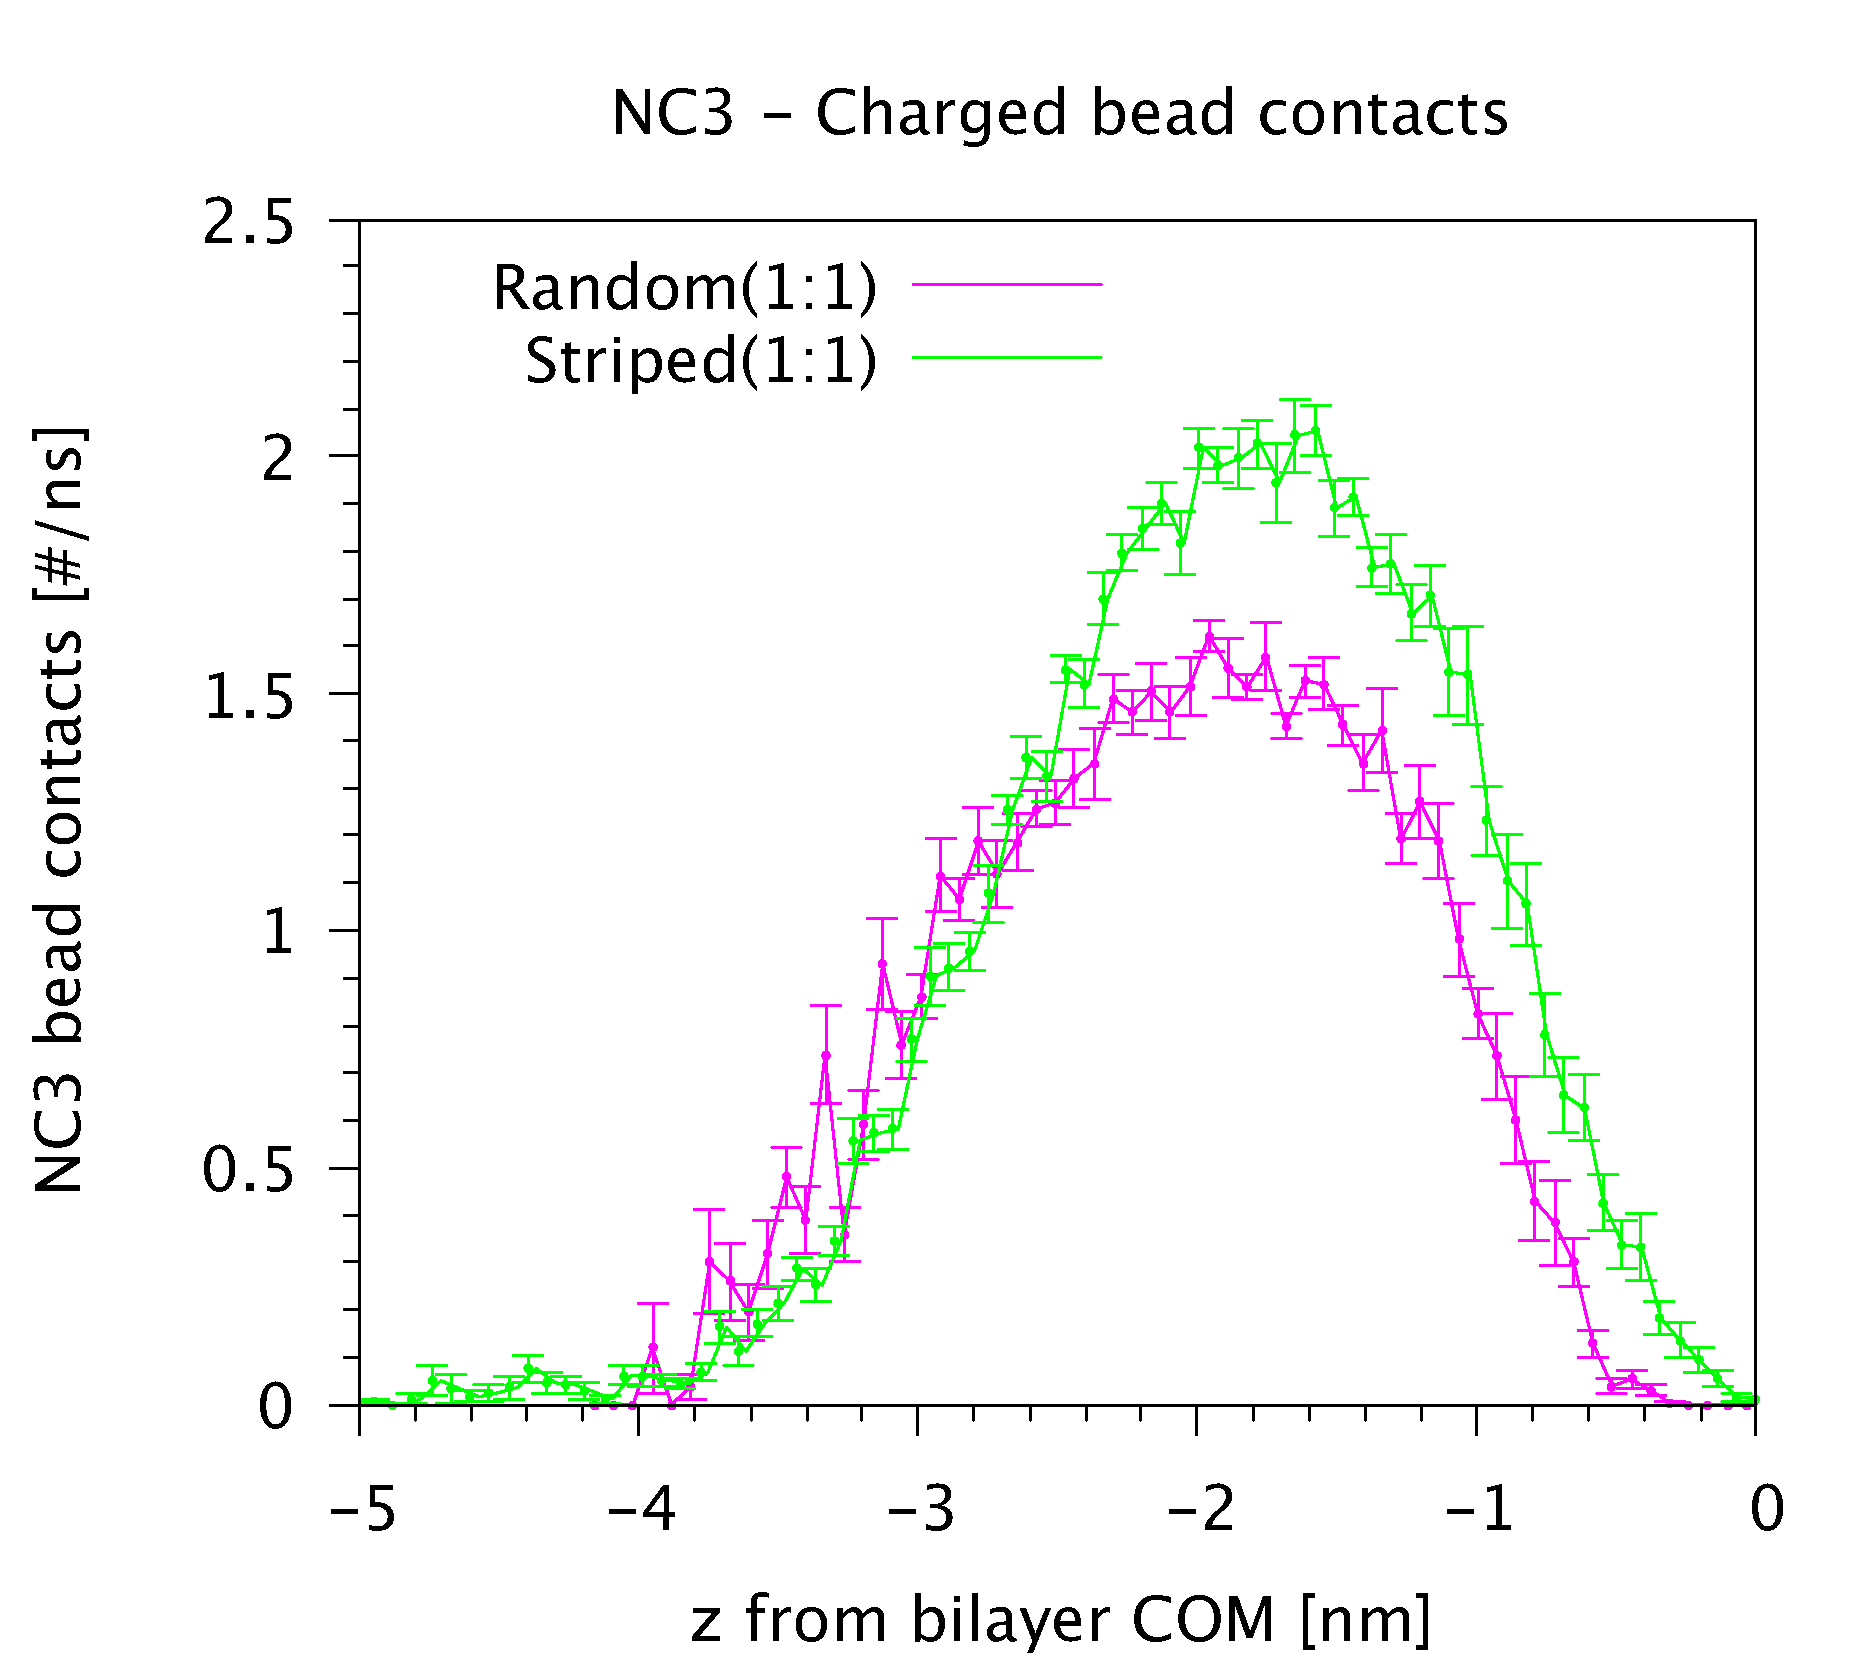
\includegraphics[width=0.5\textwidth]{./img/results/NC3RPComparison}
	}\\%
	\subfloat[Striped NP: atomistic model]{
		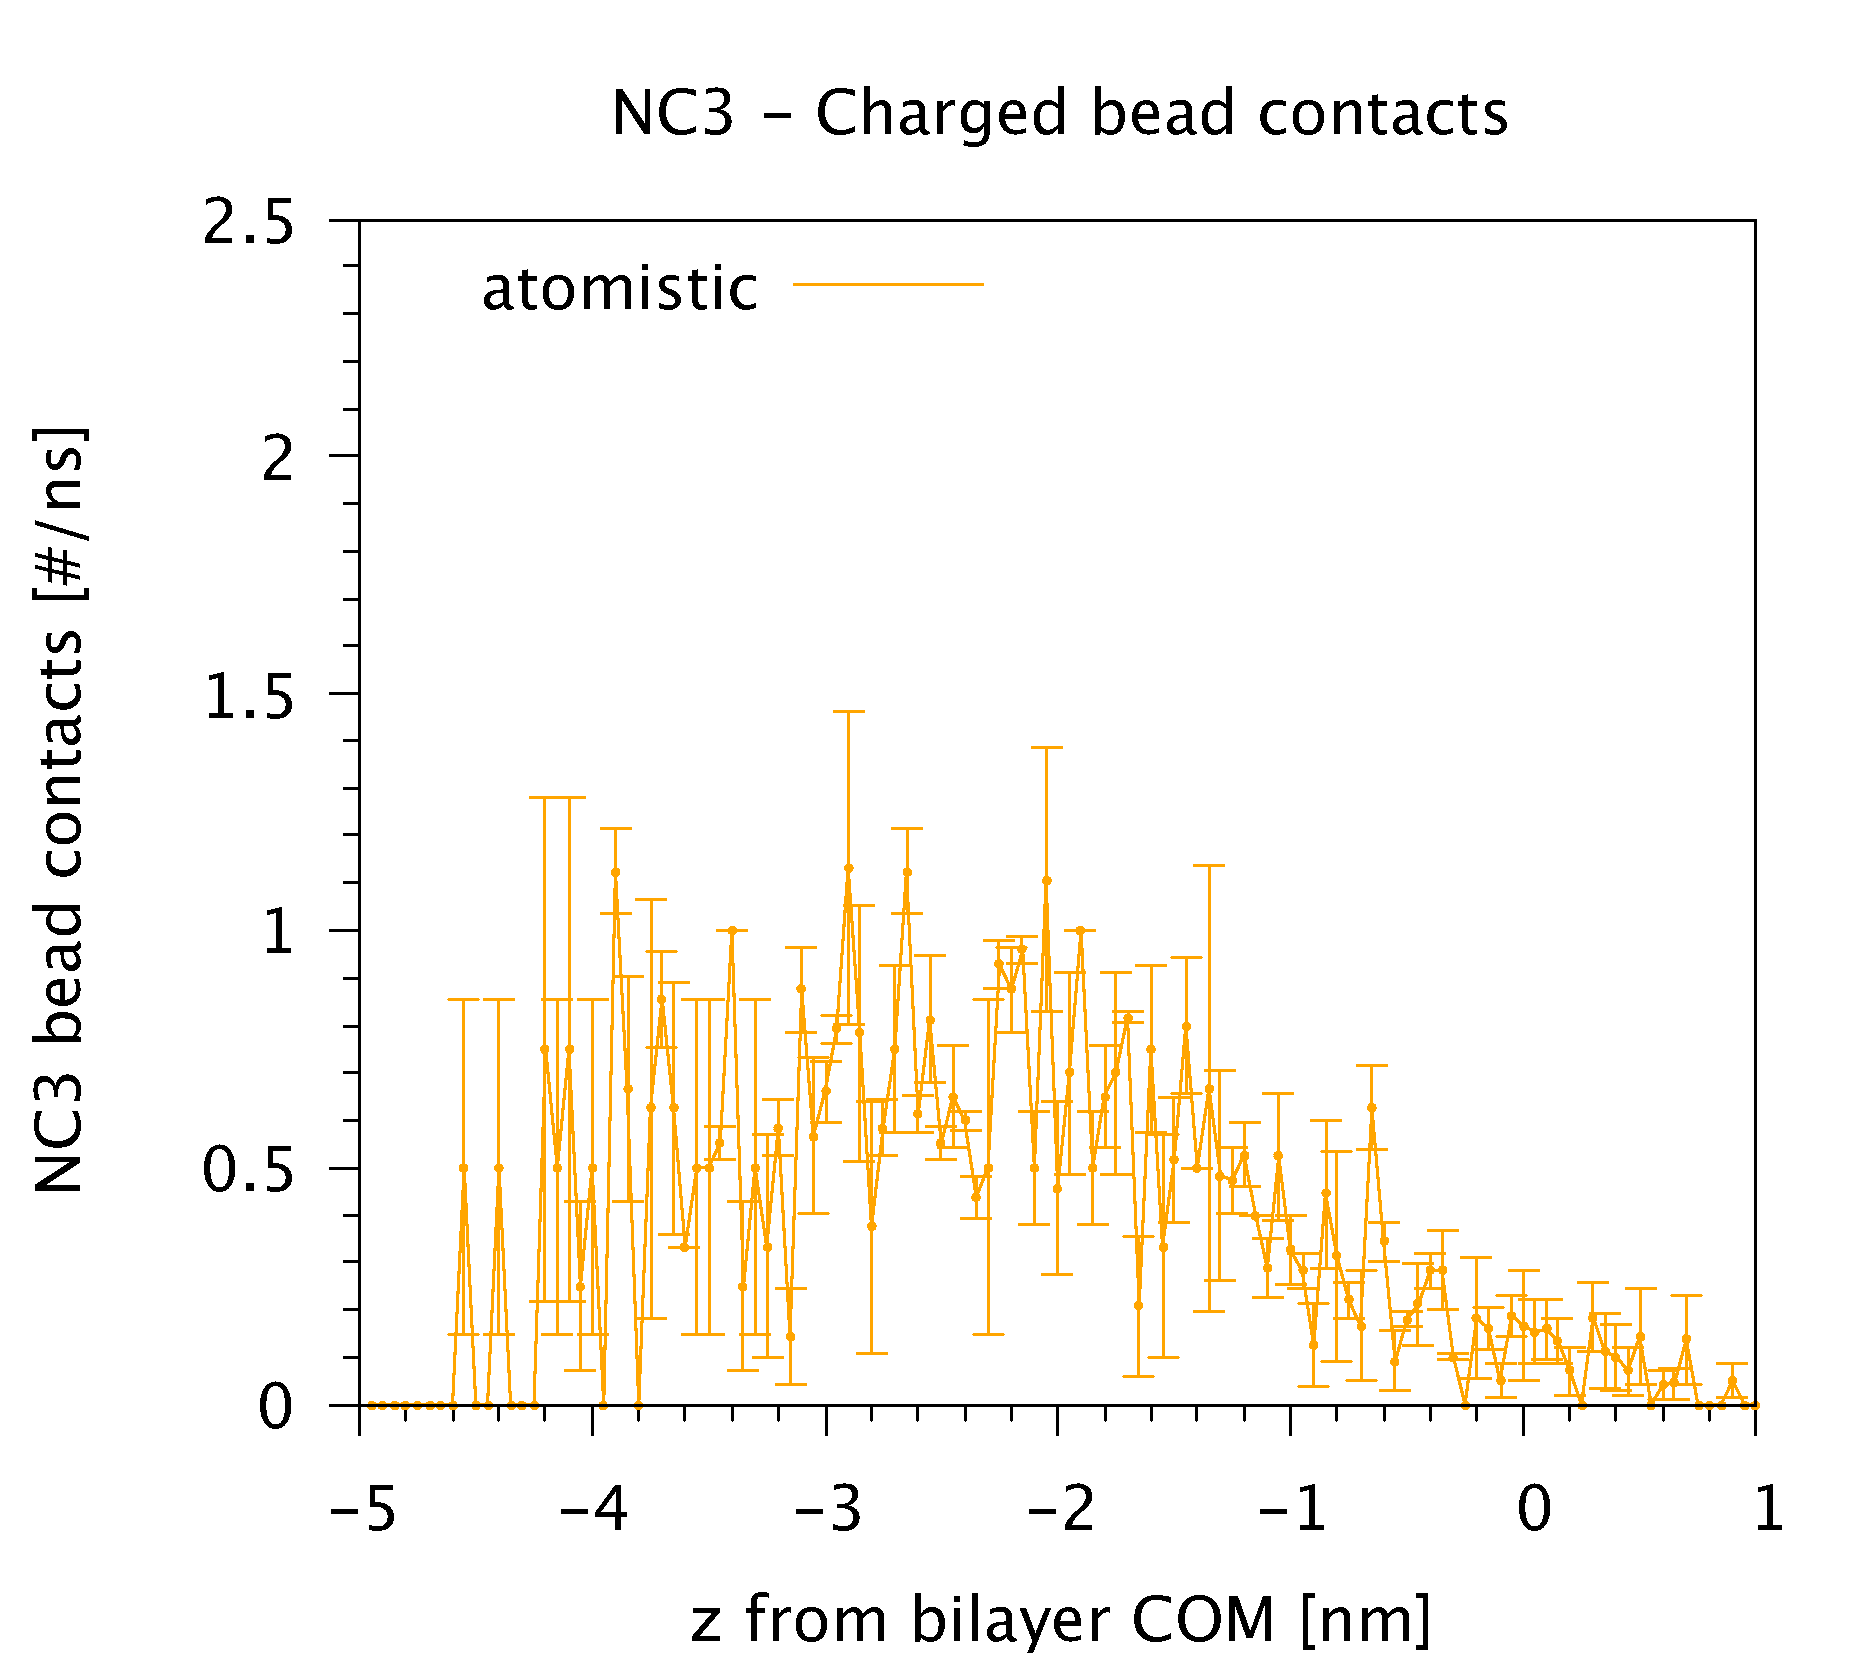
\includegraphics[width=0.5\textwidth]{./img/results/NC3PatchedAtomistic}
	}%
	\caption{Number of contacts per ns between the choline groups in the entrance leaflet and the charged ligand terminal subject to the metadynamics bias potential in function of the position of the charged ligand terminal. For $z<0$ the ligand is in the entrance leaflet. (a) For the striped \acs{NP} with different models. (b) For the striped and the random \acs{NP}s with \acs{PME} and \acs{PW}. (c) For the striped \ac{NP} with the atomistic model, (data courtesy of F. Simonelli). The \ac{CG} data are binned with a bin width of $0.08$~nm while the atomistic with a bin width of $0.05$~nm. For each histogram, the total number of counts per bin is normalized with the number of the bin entries. The error bar is the standard error of the mean value.}%
	\label{fig:NC3Contact}
\end{figure}
Moreover, the same analysis for the water contacts as described in~\ref{sec:WDragging}, is made even for the 
contacts of the choline groups in the entrance leaflet within $0.6$~nm from the charged ligand terminal. The 
results, referred to our metadynamics runs, are shown in figure~(\ref{fig:NC3Contact}). In particular, in 
figure~(\ref{fig:NC3Contact}a) is shown a comparison of the striped \ac{NP} with different \ac{CG} \martini{} 
models: the \ac{STD}, with \ac{PME} alone and with both \ac{PME} and \ac{PW}. Instead, in 
figure~(\ref{fig:NC3Contact}b) is shown a comparison between the striped and the random \acp{NP} with \ac{PME} and 
\ac{PW} and in figure~(\ref{fig:NC3Contact}c) the atomistic results for a striped \ac{NP}. We see that with the 
\ac{PW} model the contacts per ns are still appreciable even near the core of the membrane. This and the previous 
results confirm the dragging effect of the lipid heads of the entrance leaflet by the charged bead during the 
forward process. In the random--striped comparison we see that this effect is less noticeable for the random 
\ac{NP} and the number of contacts is globally lower than for the striped one. This can be consistent with the 
fact that the average $z$ distance of the \ac{NP} \ac{COM} from the bilayer \ac{COM} is shorter for the striped 
than that for the random one, as shown in table~(\ref{tab:NPMembProperties}).

\clearpage
\subsection{Effects of metadynamics}
%Quanto la metadinamica sia distrittiva: comparazione tra rum unbiased e biased
% 	minDistHydroPatched		minDistHydroRandom11
We have used metadynamics to observe the crossing of the energy barriers separating the hydrophobic contact stage 
from the anchored stage, both in forward and backward direction. It is nevertheless necessary to understand to 
what extent the
\begin{figure}[hb!]
	\center
	\subfloat[Striped NP]{
		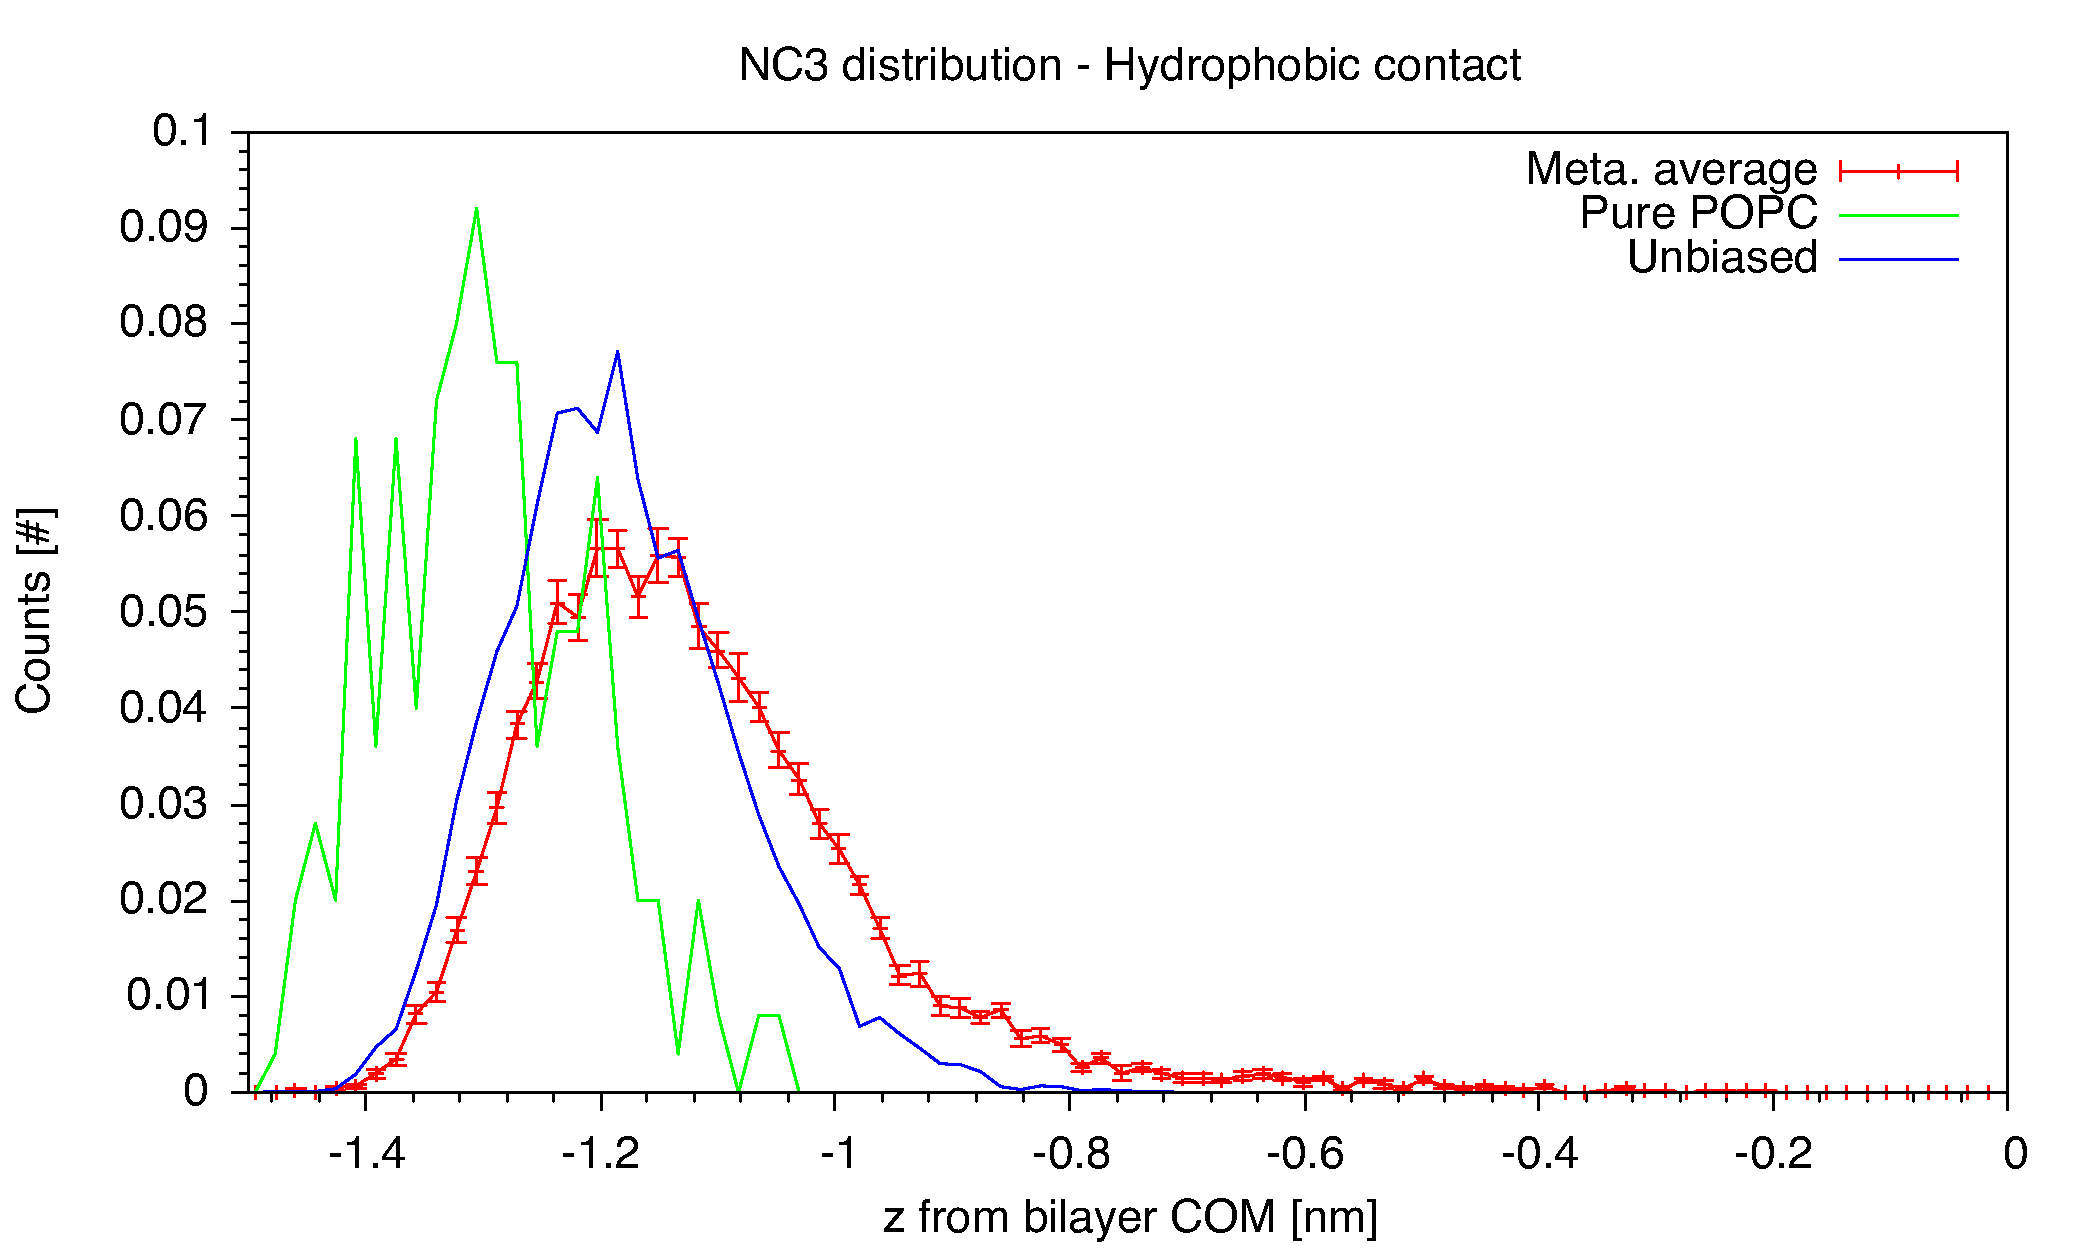
\includegraphics[width=0.85\textwidth]{./img/results/minDistHydroPatched}
	}\\%
	\subfloat[Random NP]{
		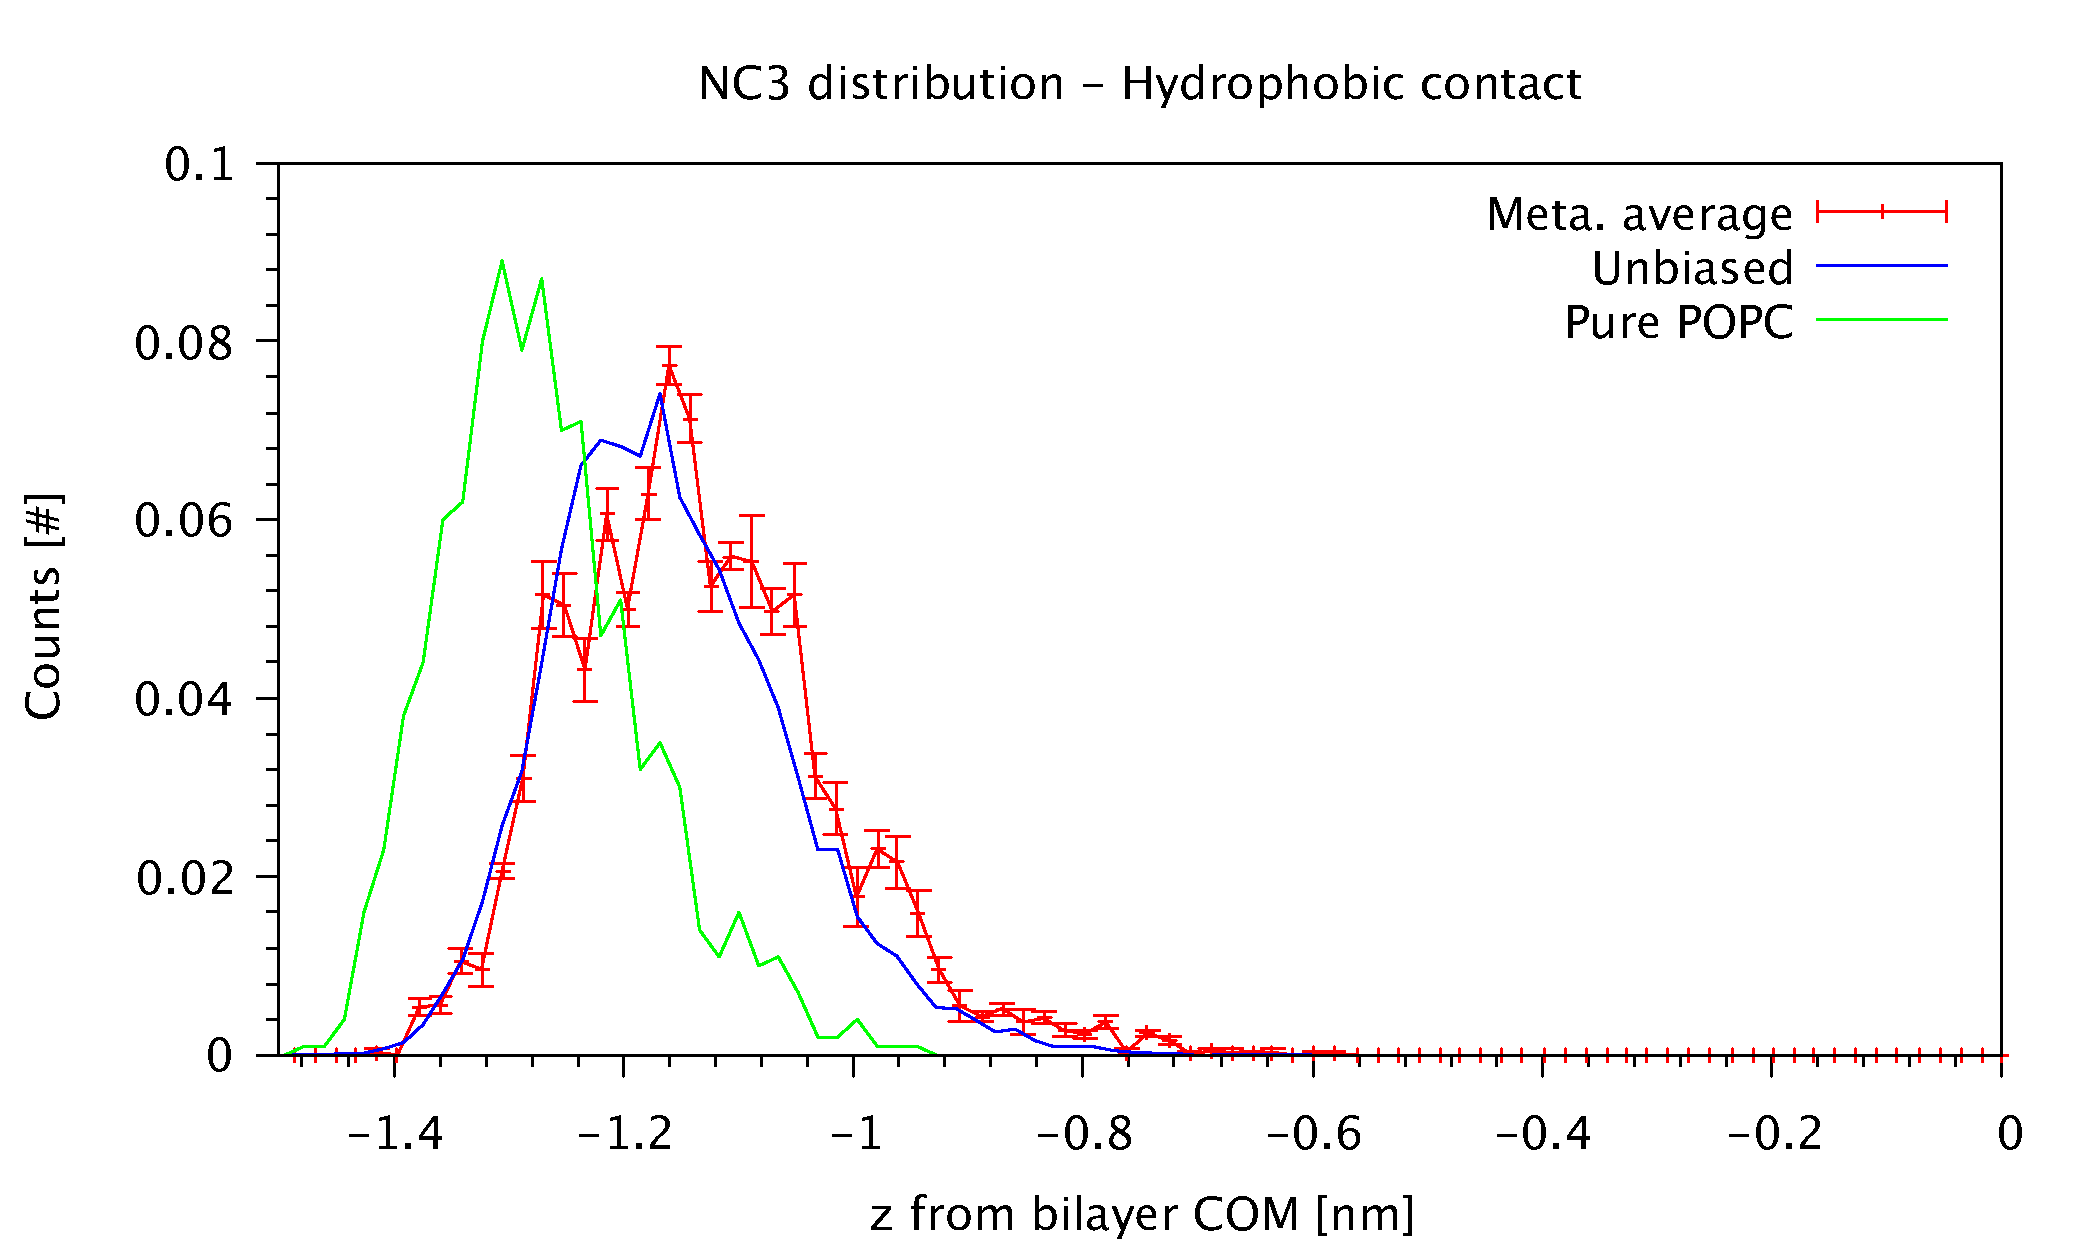
\includegraphics[width=0.85\textwidth]{./img/results/minDistHydroRandom11}
	}%
	\caption{Distribution of $d_\text{min}^{\text{NC}3}$ in the entrance leaflet. The red curve is from an average over the metadynamics runs considering only the portion of the trajectory in which the \acs{NP} is in the hydrophobic state. The blue curve is from the unbiased run and the green one is from a pure \acs{POPC} membrane. (a) For the striped \acs{NP}. (b) For the random \acs{NP}. The bin width is $0.02$~nm for all curves and each histogram is normalized to the total number of entries. The error bar for the metadynamics runs is calculated as the standard error of the mean value.}%
	\label{fig:NC3minDistUn}
\end{figure}
metadynamics biasing potential affects the molecular mechanism of the transition. In this section we are going to 
compare the structural properties of the membrane, in presence of the \ac{NP}, as measured from our metadynamics 
runs and from the unbiased runs. In figure~(\ref{fig:NC3minDistUn}) it is shown an histogram of the distribution 
of $d_\text{min}^{\text{NC}3}$ in the \ac{NP} entrance leaflet. The distribution is compared to that obtained from 
a reference pure \ac{POPC} membrane, an unbiased run and an average over the biased runs for which only the 
portion of the trajectory in which the \ac{NP} is in the hydrophobic state are considered. We observe an 
appreciable count near the hydrophobic core of the bilayer, even if only the hydrophobic state is considered. This 
suggests that the lipid head dragging is present due to the oscillation of the charged bead exploring a bigger 
area of the \ac{CV} phase space when the \ac{NP} is still in the hydrophobic state. Then, in 
figure~(\ref{fig:contactsUn}) it is shown the number of contacts per ns between the \ac{PW} beads and the charged 
ligand terminal and between the choline groups and the charged ligand terminal of a striped and a random \acp{NP} 
for the biased runs in comparison with the unbiased runs. These analysis are made considering only the 
\ac{PME}+\ac{PW} model. From figure~(\ref{fig:contactsUn}) we see that the number of contacts are almost equal in 
the hydrophobic state for all plots, suggesting that the metadynamics is non--destructive.
%	patchedPWContact	randon11PWContact
% 	patchedNC3Contact	random11NC3Contact
\begin{figure}[ht!]
	\center
%	\begin{adjustwidth}{-0.5cm}{-1.5cm}
		\subfloat[Striped NP]{
		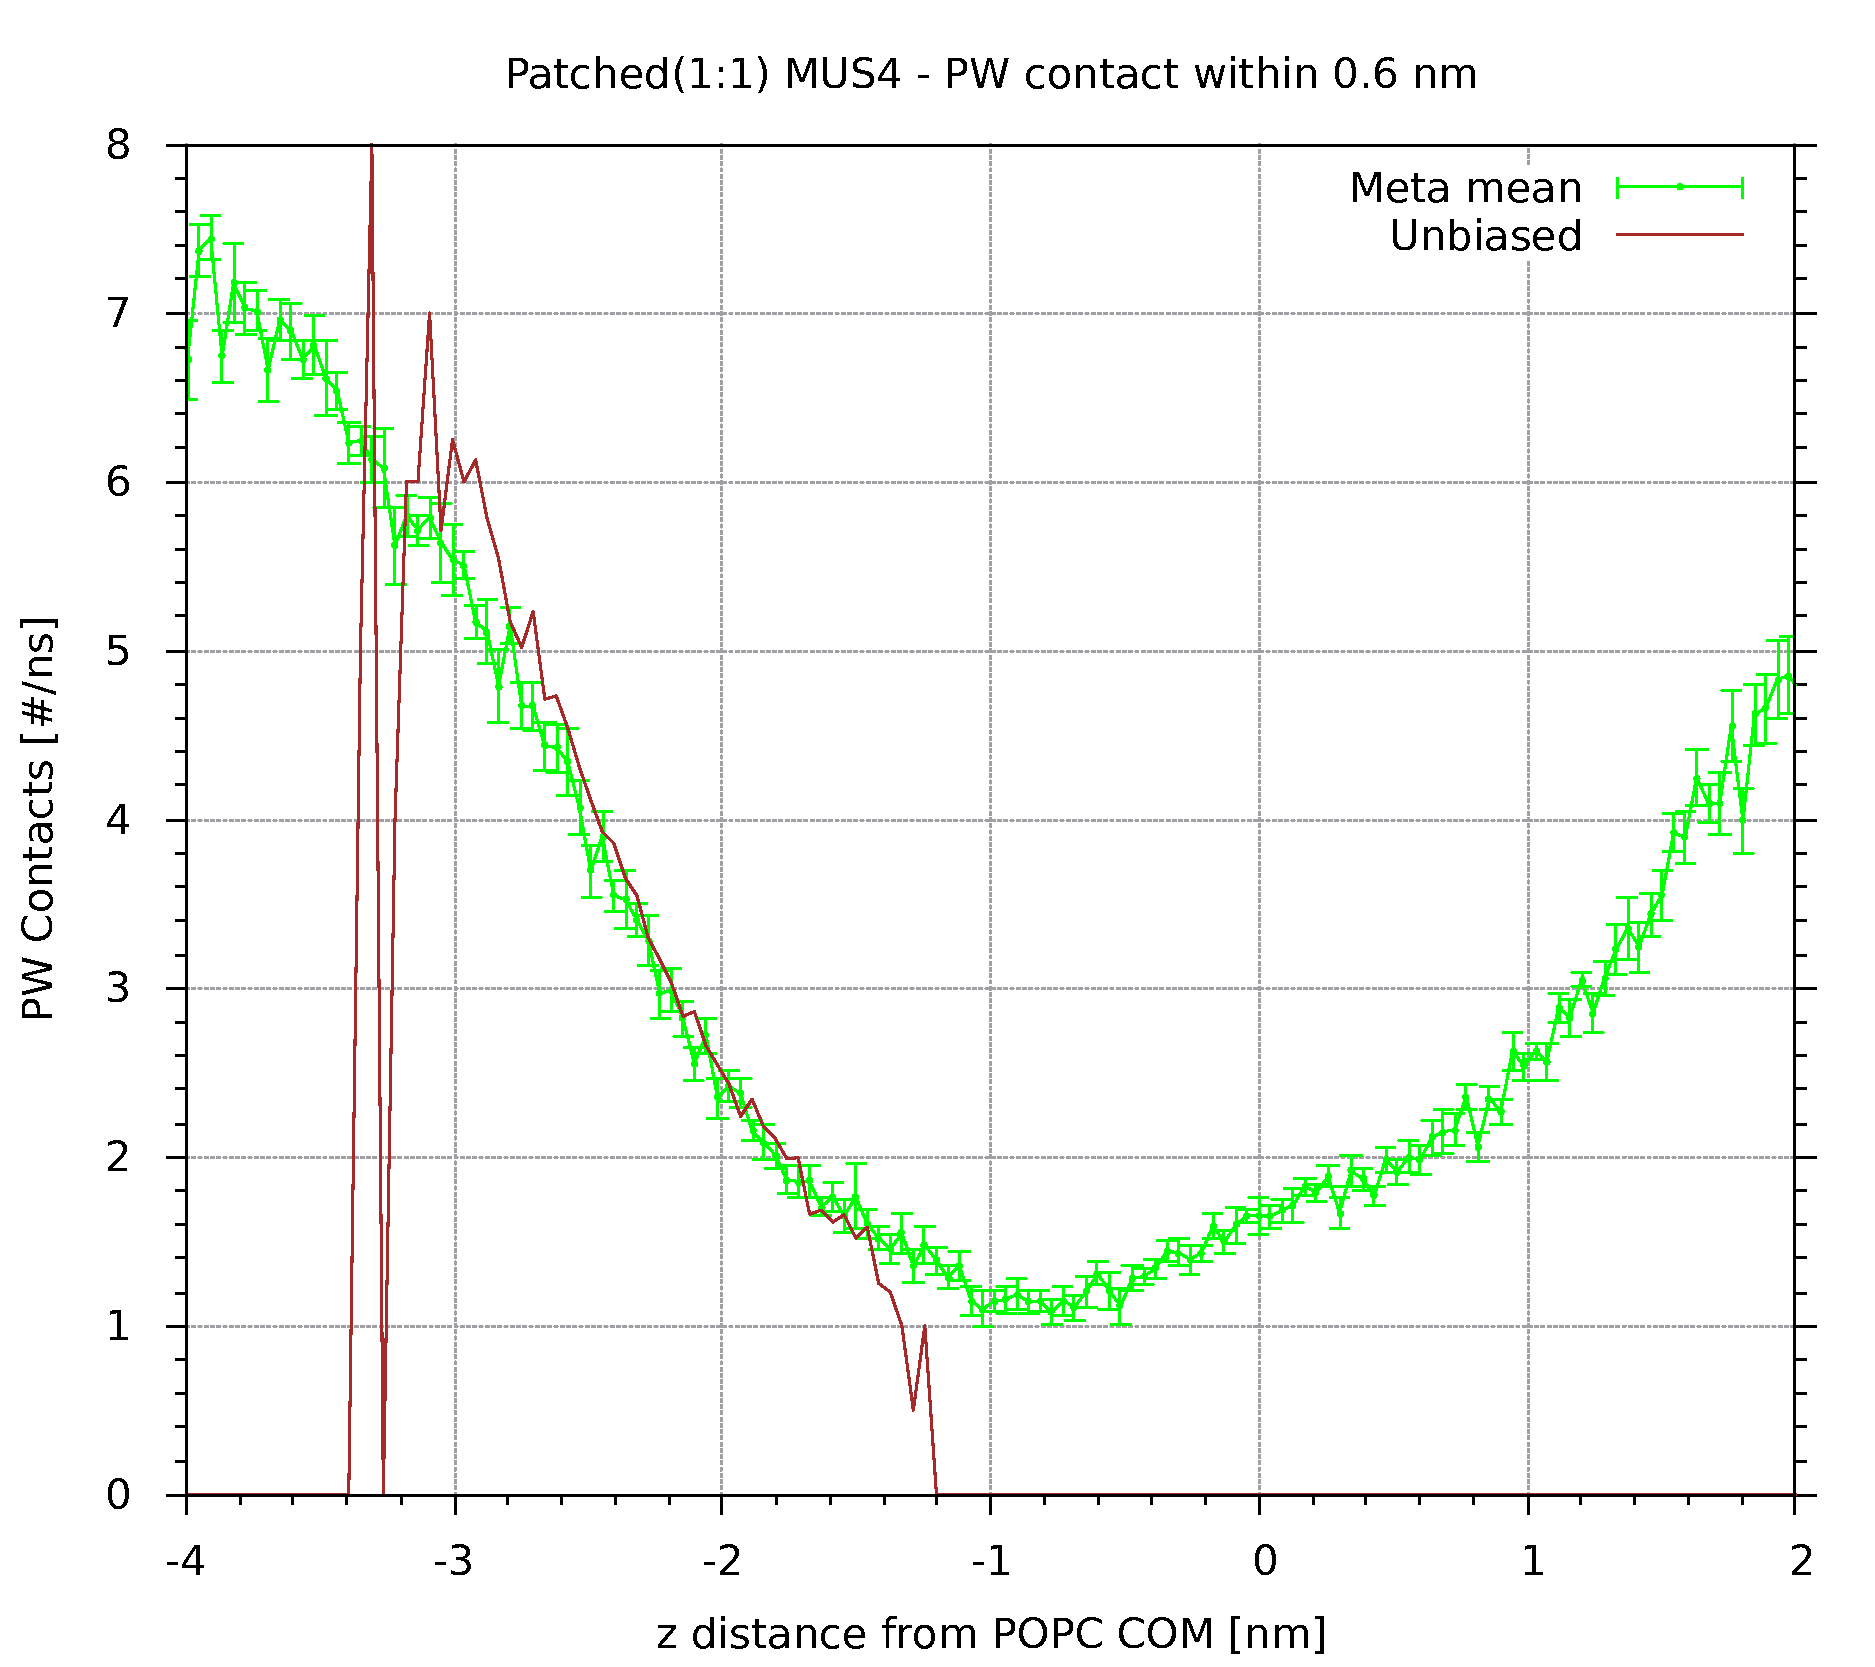
\includegraphics[width=0.5\linewidth]{./img/results/patchedPWContact}
		}%
		\subfloat[Random NP]{
		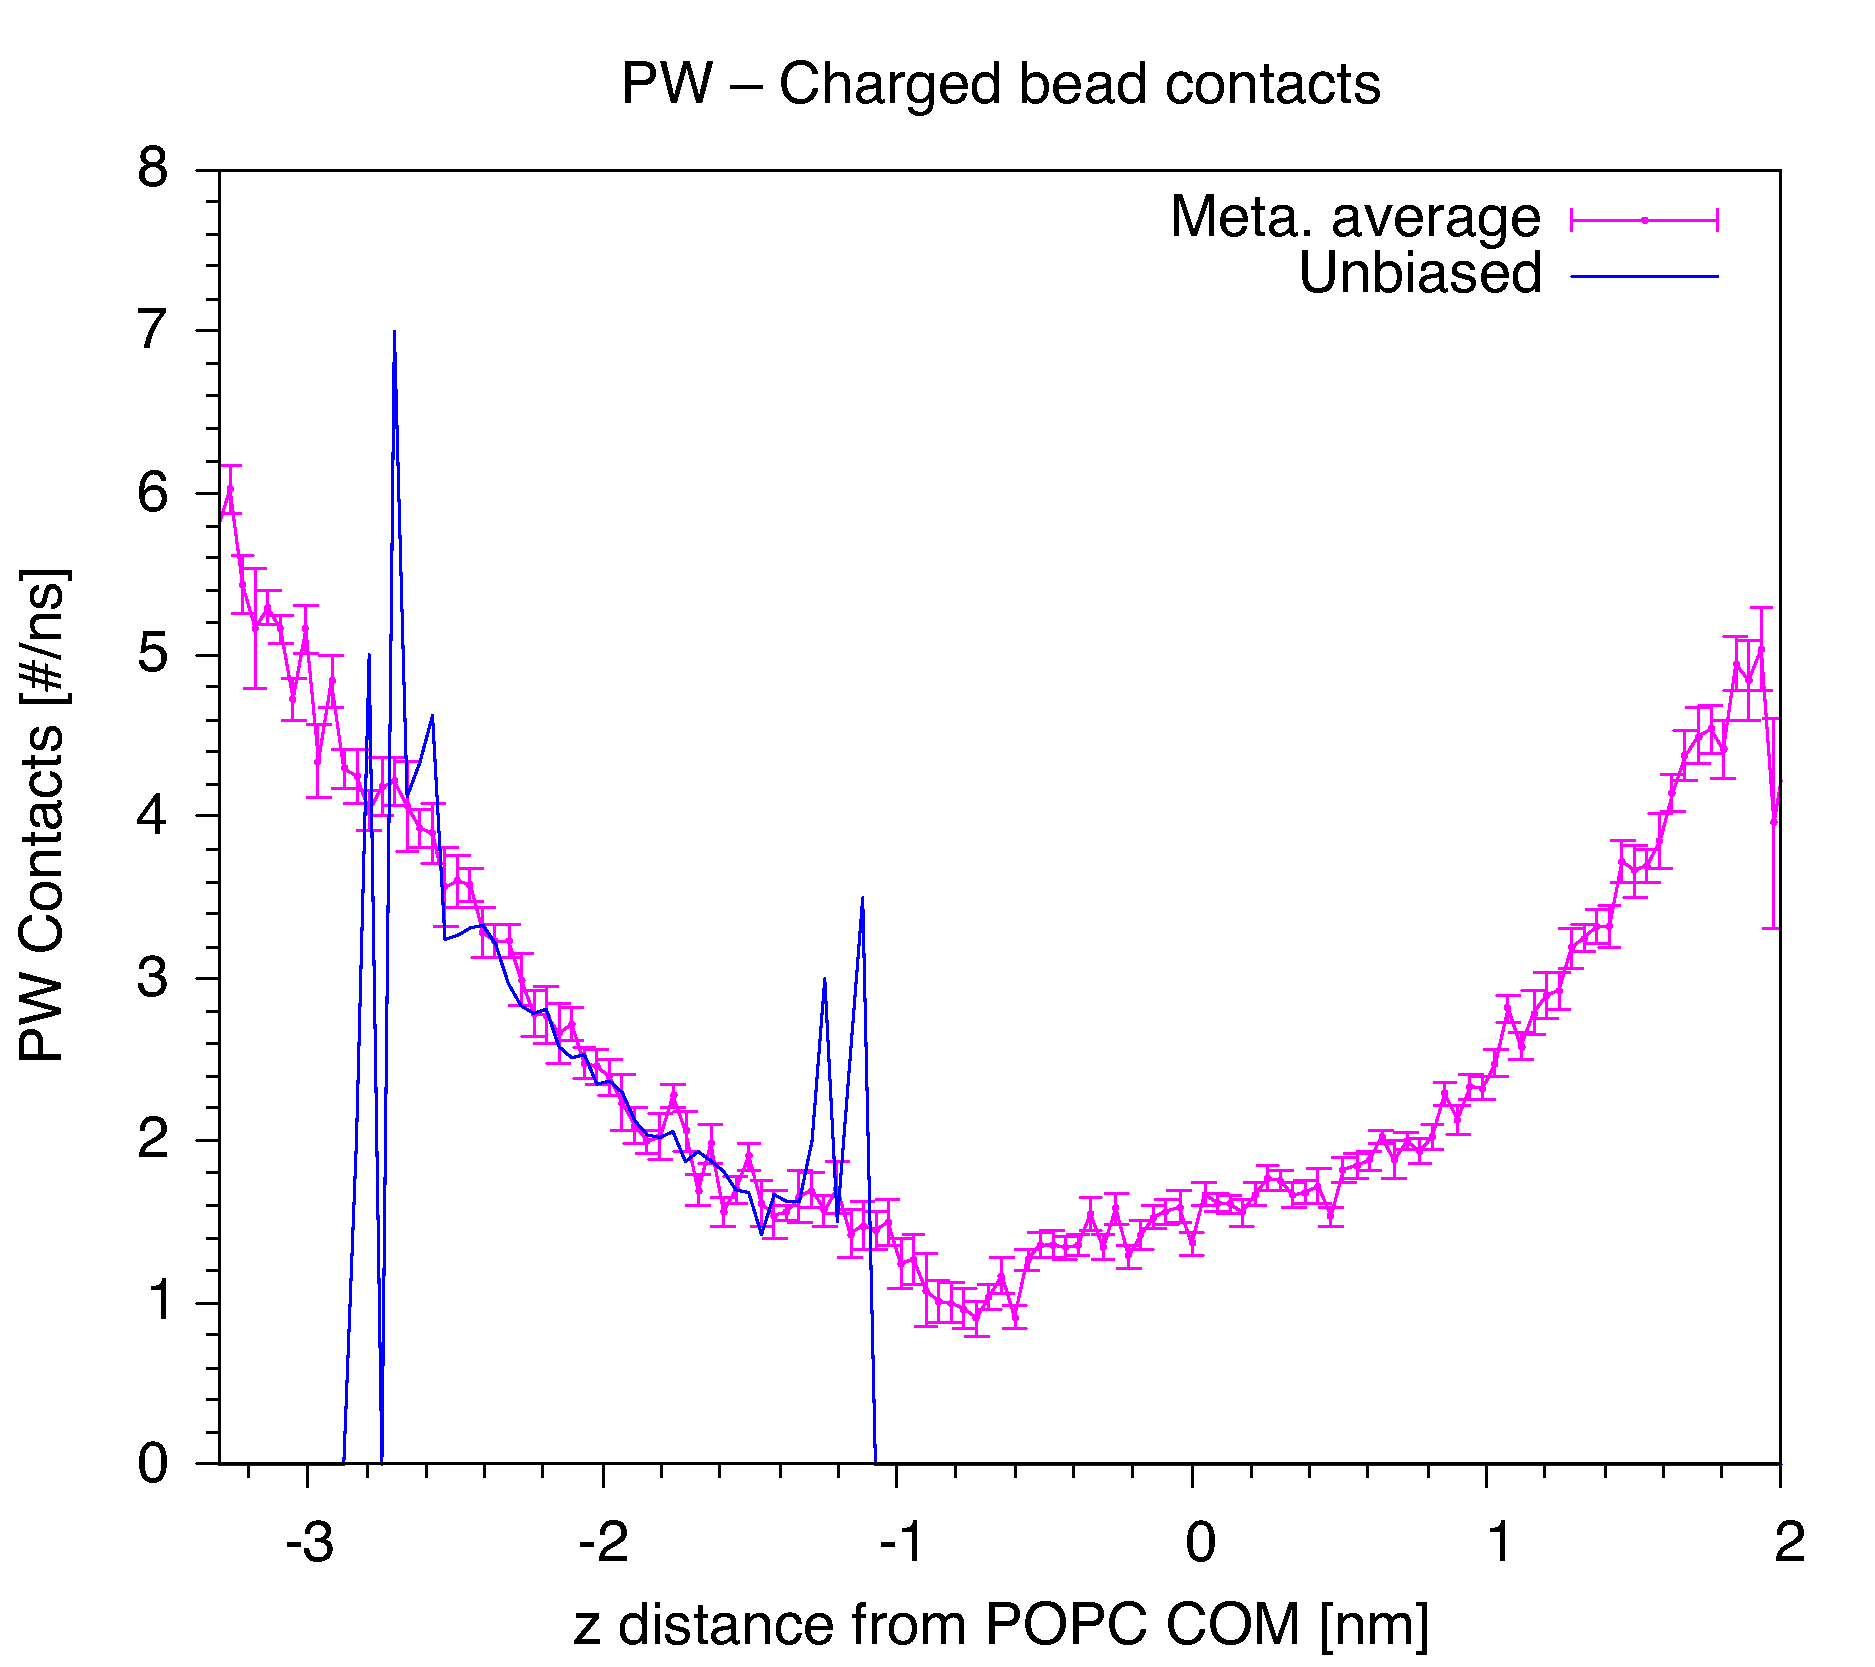
\includegraphics[width=0.5\linewidth]{./img/results/random11PWContact}
		}\\%
		\subfloat[Striped NP]{
		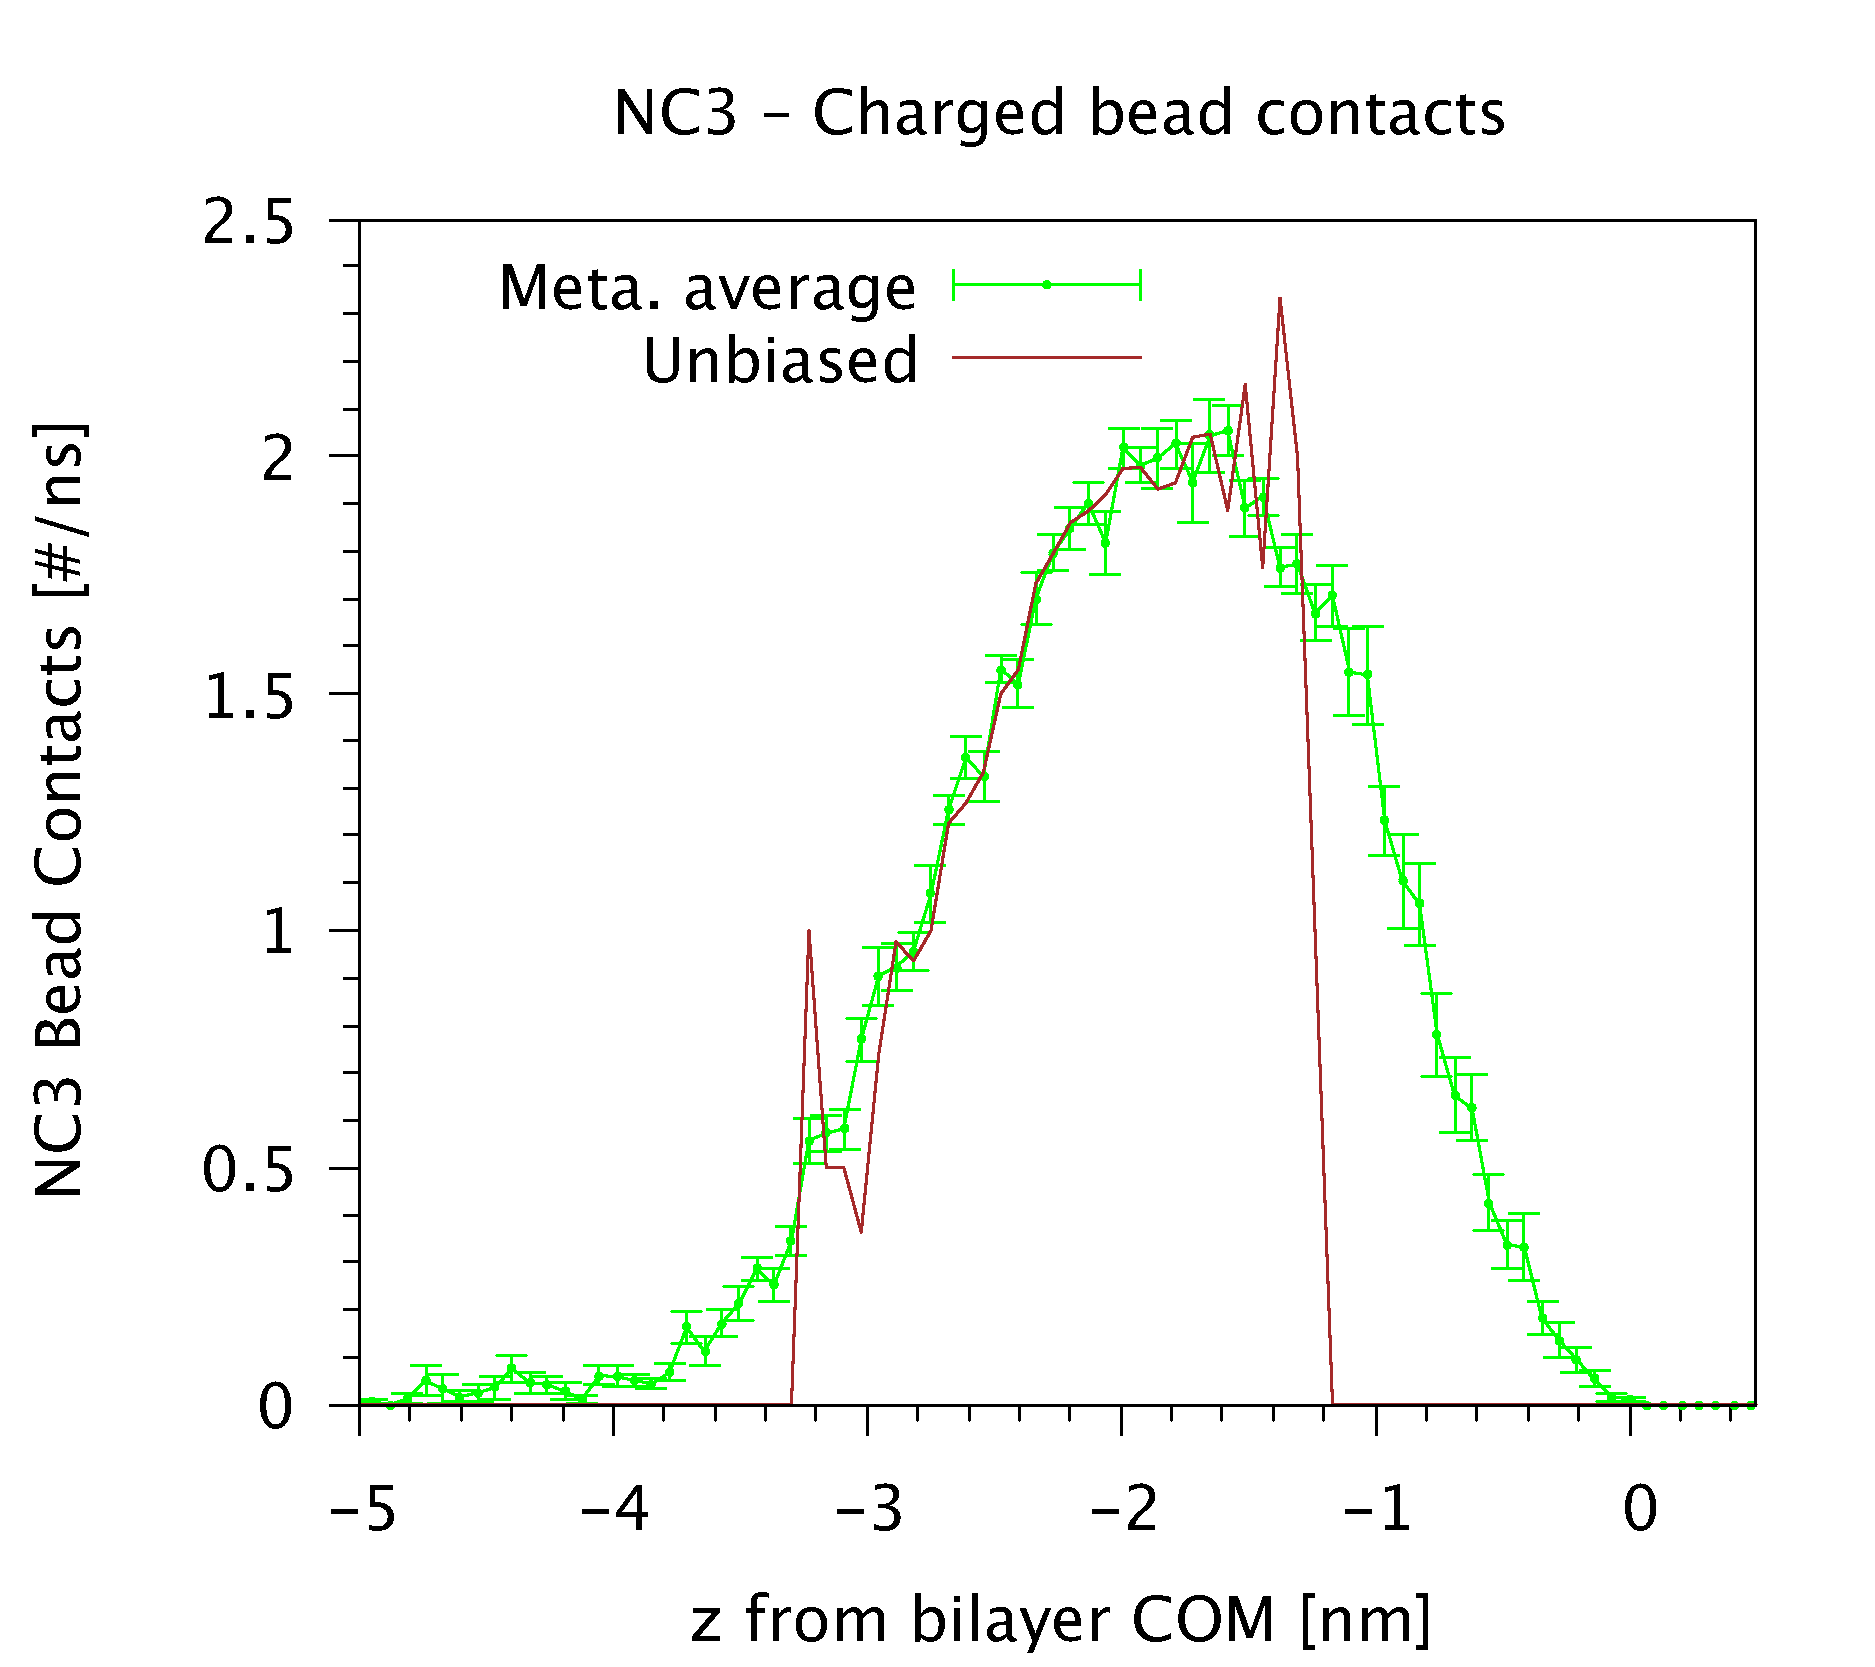
\includegraphics[width=0.5\linewidth]{./img/results/patchedNC3Contact}
		}%
		\subfloat[Random NP]{
		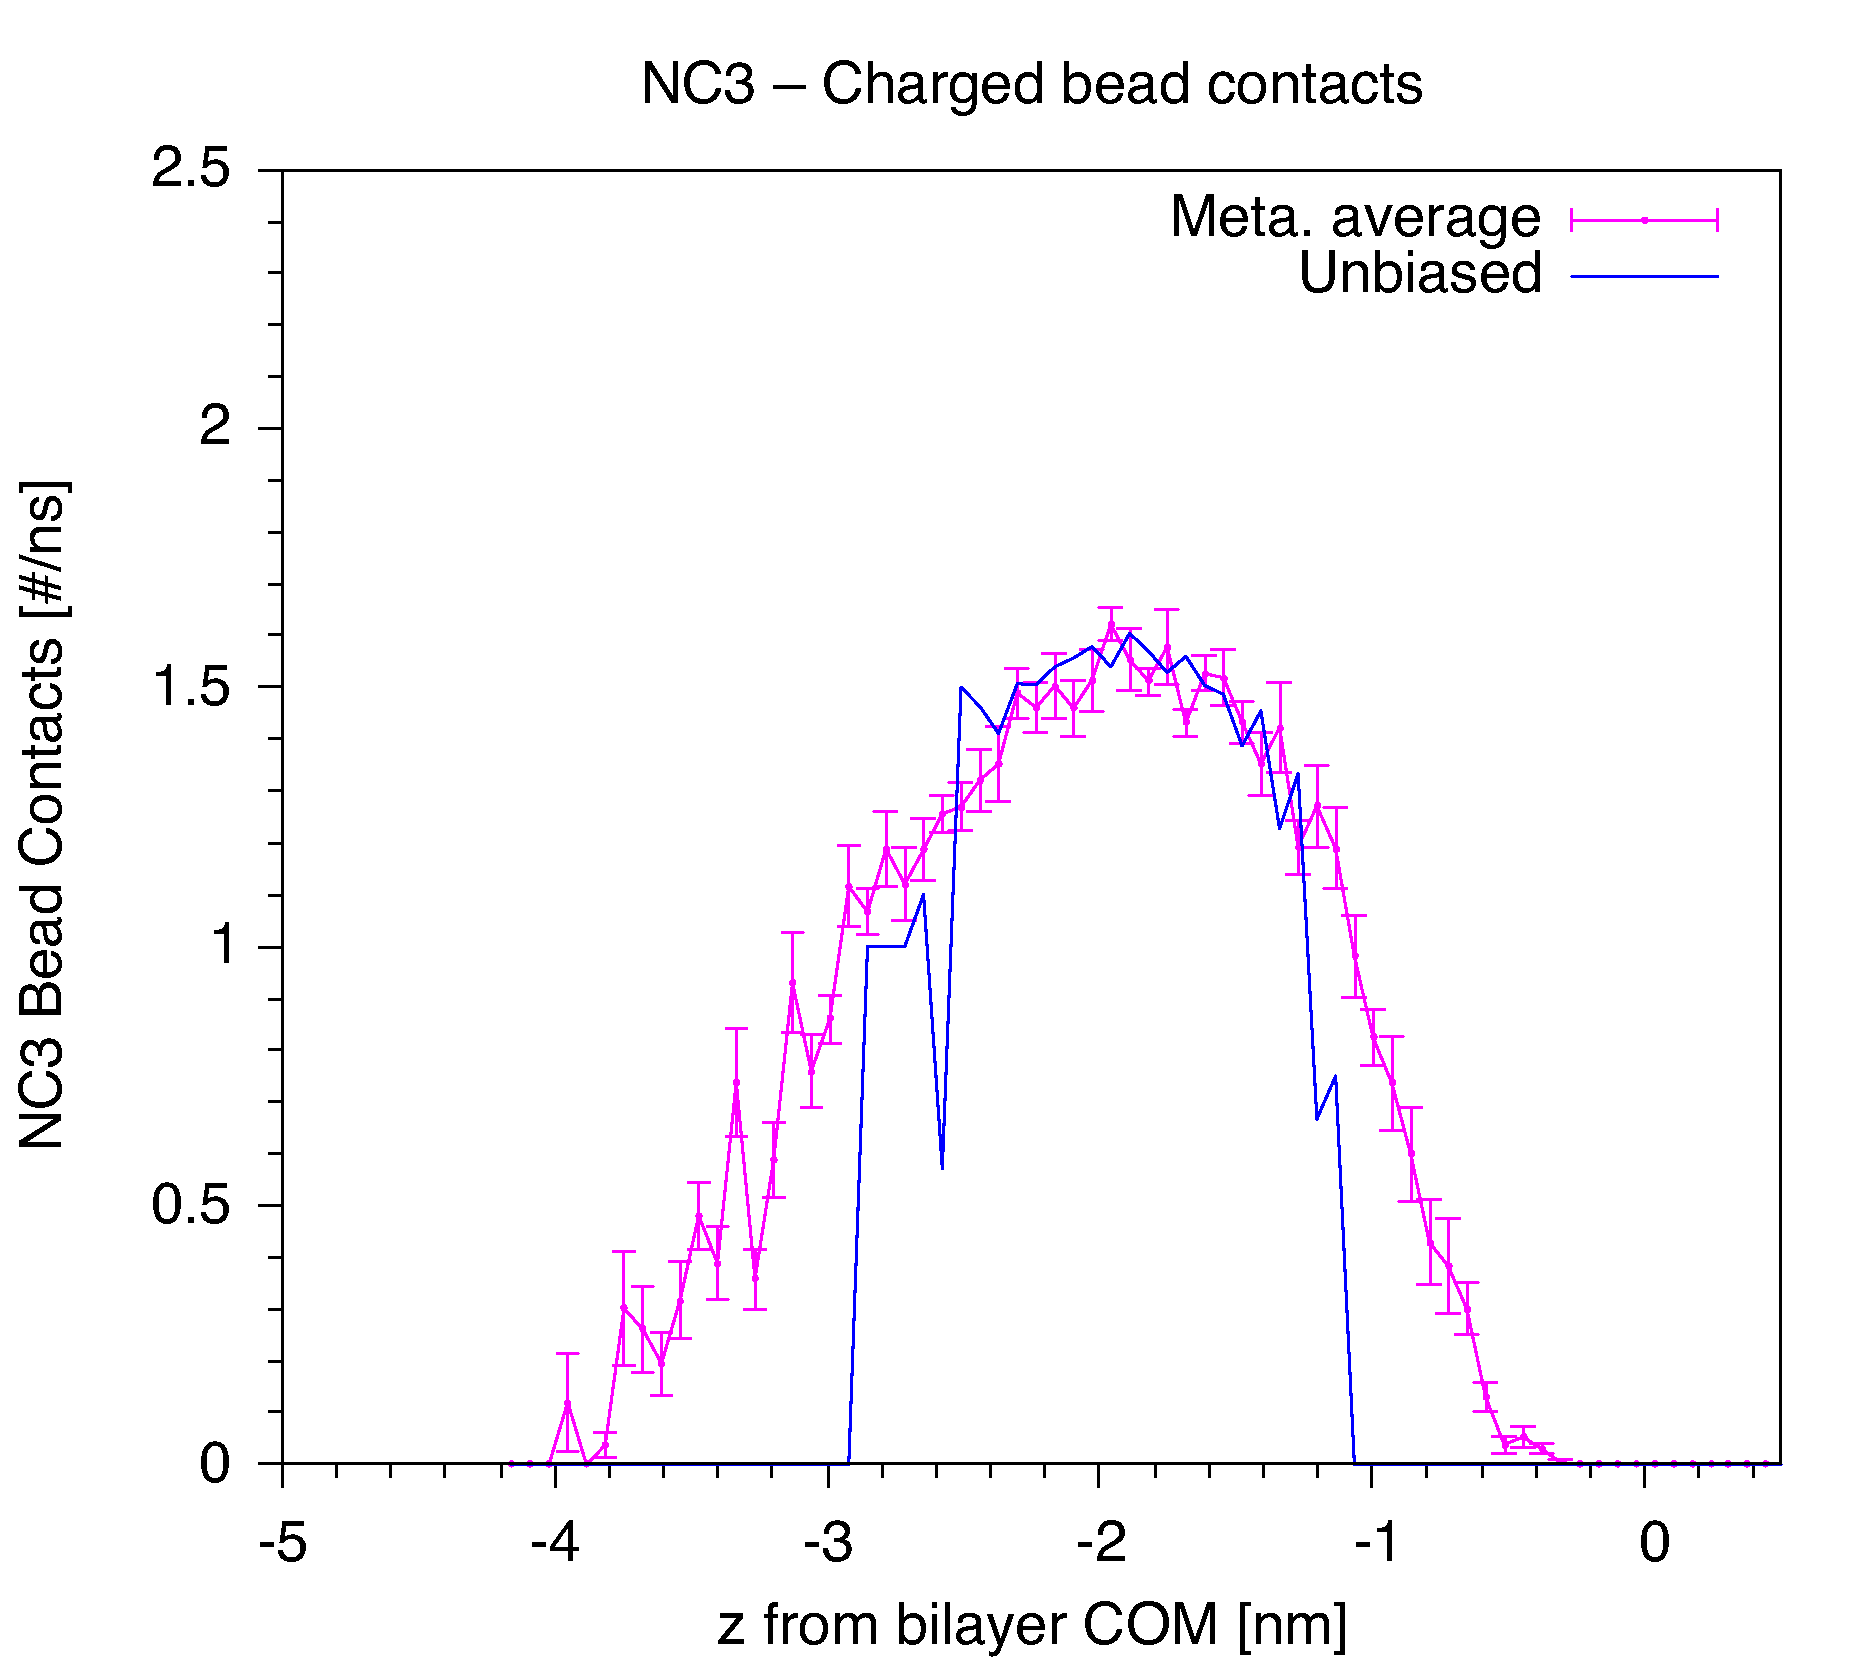
\includegraphics[width=0.5\linewidth]{./img/results/random11NC3Contact}
		}
		\caption{(a-b) Number of contacts per ns between the \acs{PW} beads and the charged bead in function of the position of the charged ligand terminal for: (a) the striped \acs{NP} and (b) the random \acs{NP}. (c-d) The same for the choline group and the charged ligand terminal in the hydrophobic state for: (c) the striped \ac{NP} and (d) the random \acs{NP}. For each plots the number of contacts are in comparison with the corresponding unbiased runs. $z<0$ corresponds to the entrance leaflet. The biased data are binned with a bin width of $0.08$~nm and the total number of counts per bin is normalized with the number of the bin entries. The error bar is the standard error of the mean value.}%
		\label{fig:contactsUn}
%	\end{adjustwidth}
\end{figure}

\clearpage
\section{NP and membrane properties}
%Proprietà generali
%Coef di diffusione stato ancorato, stato idrofobico
To complete the set of analysis on the interaction between the \acp{NP} and the model lipid membrane with the 
\martini{} \ac{FF} with \ac{PME}$+$\ac{PW} model, we investigate the effect on the membrane properties, such as 
the lipid diffusion coefficient and the density map of the lipids treating the \ac{NP} entrance leaflet and the 
anchoring leaflet, separately. Eventually, we consider also the \ac{NP}--lipid heads and the \ac{NP}--lipid tails 
$2$D--\ac{RDF} along the $xy$--plane, separately for the two leaflets.

In the following first some general analysis of the \acp{NP} and the bilayer lipids are given. Then we investigate the membrane properties.

\paragraph{\textbf{General properties}} For each of the unbiased runs of the different \ac{NP} configurations in 
the hydrophobic state, I show in table~(\ref{tab:NPMembProperties}) some general properties about the \ac{NP} and 
the bilayer. In particular, $\overline{d_z}$ is the average over time of the $z$ component of the distance between 
the \ac{COM} of the \ac{NP} and the \ac{COM} of the bilayer: the striped configuration is the one closest to the 
bilayer center. Moreover, I have calculated the lateral diffusion coefficient of the \ac{NP} and of the \ac{POPC} 
lipids separately for the two leaflets. We see that the striped \ac{NP} shows the fastest diffusion rate. For what 
concern the lipids, if we compare this result to the one showed in table~(\ref{tab:POPCData}), we see a general 
slow down of the diffusion rate of the lipids in presence of the \ac{NP}, with the slowest diffusion rate of the 
lipids in the \ac{NP} entrance leaflet.
\begin{table}[h!t]
	\centering\footnotesize
	\begin{tabular}{lcccc}
		\toprule
		\,		& striped ($1$:$1$)		& random ($1$:$1$)		& random ($2$:$1$)	& striped ($1$:$1$)	\\
		\,		& \acs{PW}$+$\acs{PME}$^a$ & \acs{PW}$+$\acs{PME}$^a$ & \acs{PW}$+$\acs{PME}$^a$ & atomistic$^b$ \\ \toprule
		$D^h_{\text{NP}}$ [$10^{-8}$~cm$^2$/s] & $12$ & $5$ & $5.7$ & –		 \\ \midrule
		$D_{el}$ [$10^{-8}$~cm$^2$/s] & $22 \pm 2$ & $25 \pm 1$ & $27.8 \pm 0.1$ & $8.2 \pm 0.2$	\\ \midrule
		$D_{al}$ [$10^{-8}$~cm$^2$/s] & $30 \pm 1$ & $27 \pm 3$	& $35 \pm 1$	& $6.8 	\pm 0.1$		\\ \midrule
		$\overline{d_z}$ [nm] & $1.996 \pm 0.0016$	& $2.2794 \pm 0.0017$	& $2.7284 \pm 0.0014$	& $1.708 \pm 0.008$\\ \bottomrule
	\end{tabular}
	\caption{Lateral diffusion coefficients: of the \acs{NP} in the hydrophobic state ($D^h_\text{NP}$), of the lipids in the entrance leaflet ($D_{el}$) and in the anchoring leaflet ($D_{al}$). $\overline{d_z}$ is the average $z$ component of the distance between the \acs{COM} of the \acs{NP} and the \acs{COM} of the \acs{POPC} bilayer. $^a$ Data obtained from my unbiased runs. $^b$ Data courtesy of F. Simonelli.}%
	\label{tab:NPMembProperties}
\end{table}

\paragraph{\textbf{Bilayer structural properties}}
%Risucchio delle membrane al recrossing
%Deformazione del leaflet di ancoraggio: RDF e densitymap 2D
In my biased and unbiased \ac{MD} runs with the \martini{} \ac{PME}$+$\ac{PW} model, the main membrane structural 
deformation is related to an evident distortion of the leaflet that does not host the \ac{NP}, as it is shown in 
figure~(\ref{fig:engulfmentFrame}). This effect is in agree with the atomistic simulation. The opposite leaflet 
deformation related to the metadynamics run, figure~(\ref{fig:engulfmentFrame}e-f), is clearly more accentuated 
due to the strong electrostatic interaction between the charged ligand terminal and the choline groups of the 
anchoring leaflet. As a consequence, during the backward process, the charged ligand terminal drag the anchoring 
leaflet before the dis--anchor can occurs. Moreover, as one can see from figure~(\ref{fig:engulfmentFrame}), the 
leaflet deformation seems to be clearly related to the distance between the \ac{COM} of the \ac{NP} and the lipid 
membrane along the bilayer normal.

For the striped (\ac{MUS}:\ac{OT} $1$:$1$), the random (\ac{MUS}:\ac{OT} $1$:$1$) and the random (\ac{MUS}:\ac{OT} 
$2$:$1$) \acp{NP} in the hydrophobic state of my unbiased runs the numerical density of lipids in the \ac{NP} 
entrance leaflet and in the opposite one is considered separately. In figures~(\ref{fig:stripedDensity}), 
(\ref{fig:randomDensity}) and~(\ref{fig:random21Density}) the $2$D--density plots are obtained from averages of 
the number density values in the box volume over time and $z$--axis. Instead, figure~(\ref{fig:RDF}) shows the 
$2$D--\ac{RDF} along the $xy$--plane of the \ac{NP}--lipid heads and the \ac{NP}--lipid tails, separately for both 
leaflets. For all the \ac{NP} configurations we see an increase of the density of the lipid heads in the opposite 
leaflet as a result of the lipid heads clustering under the \ac{NP}. As a consequence, the lipid tails of the 
opposite leaflet accumulate in a circular corona around the \ac{NP}. For what concerns the entrance leaflet we 
observe an opposite behavior. The lipid heads, especially the positively charged choline groups, are 
electrostatically attracted to the negatively charged \ac{MUS} ligands, hence the choline groups cluster in a 
circular corona at the edge of the \ac{NP}. The lipid tails of the entrance leaflet, instead, are placed 
immediately below the \ac{NP} since they are strongly attracted to the hydrophobic \ac{OT} ligands attached to the 
\ac{NP} core. This behavior produces the opposite leaflet deformation as shown in 
figure~(\ref{fig:engulfmentFrame}).

\begin{figure}[ht!]
	\center
		\subfloat[\ac{CG} unbiased run]{%
			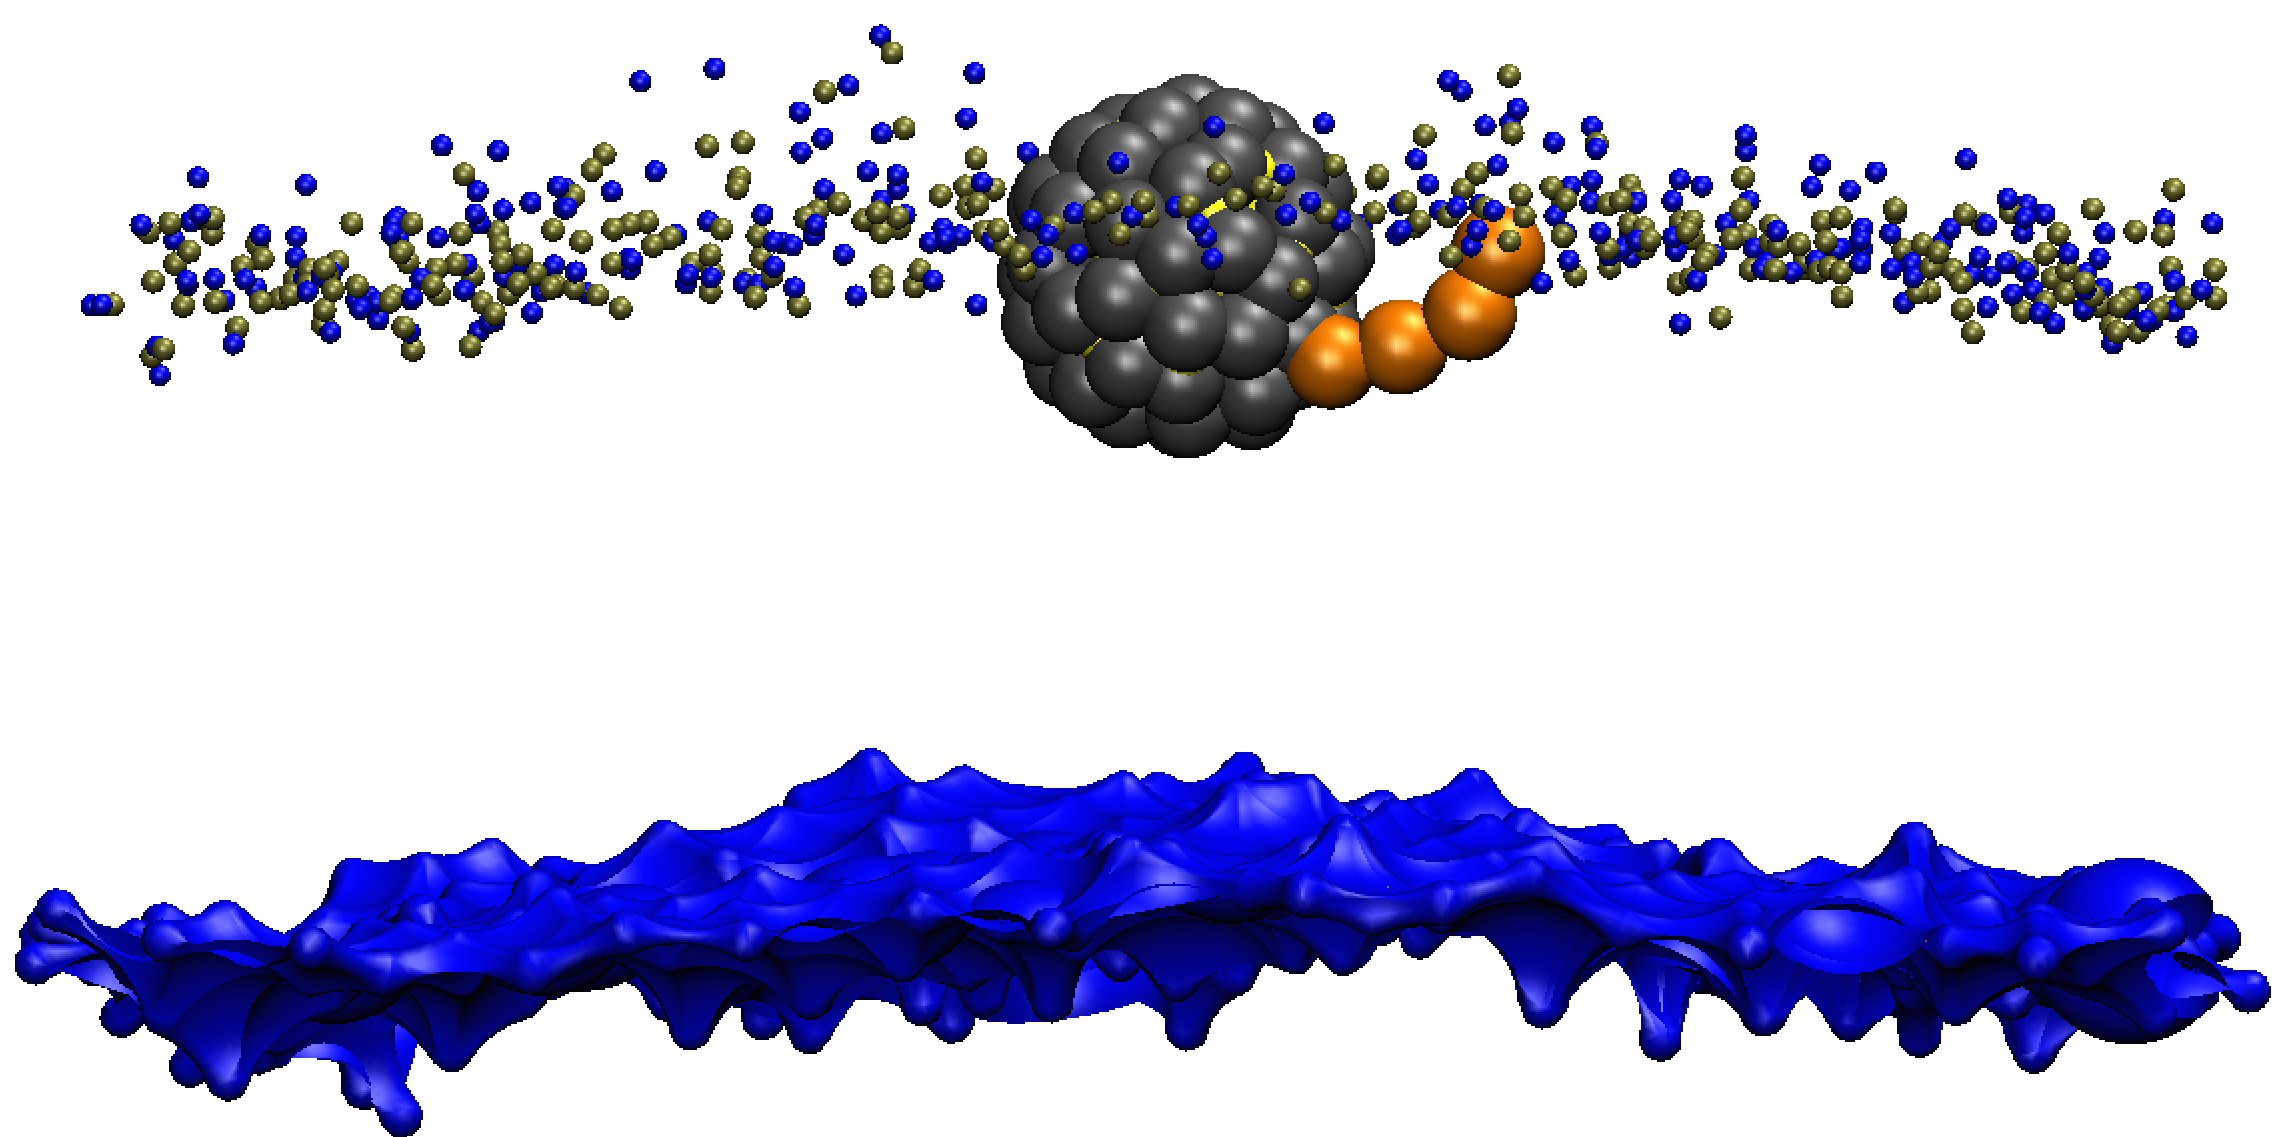
\includegraphics[width=0.47\linewidth]{./img/engulfmentFrame/a.png}%
		}\ %
		\subfloat[\acs{CG} unbiased run]{
			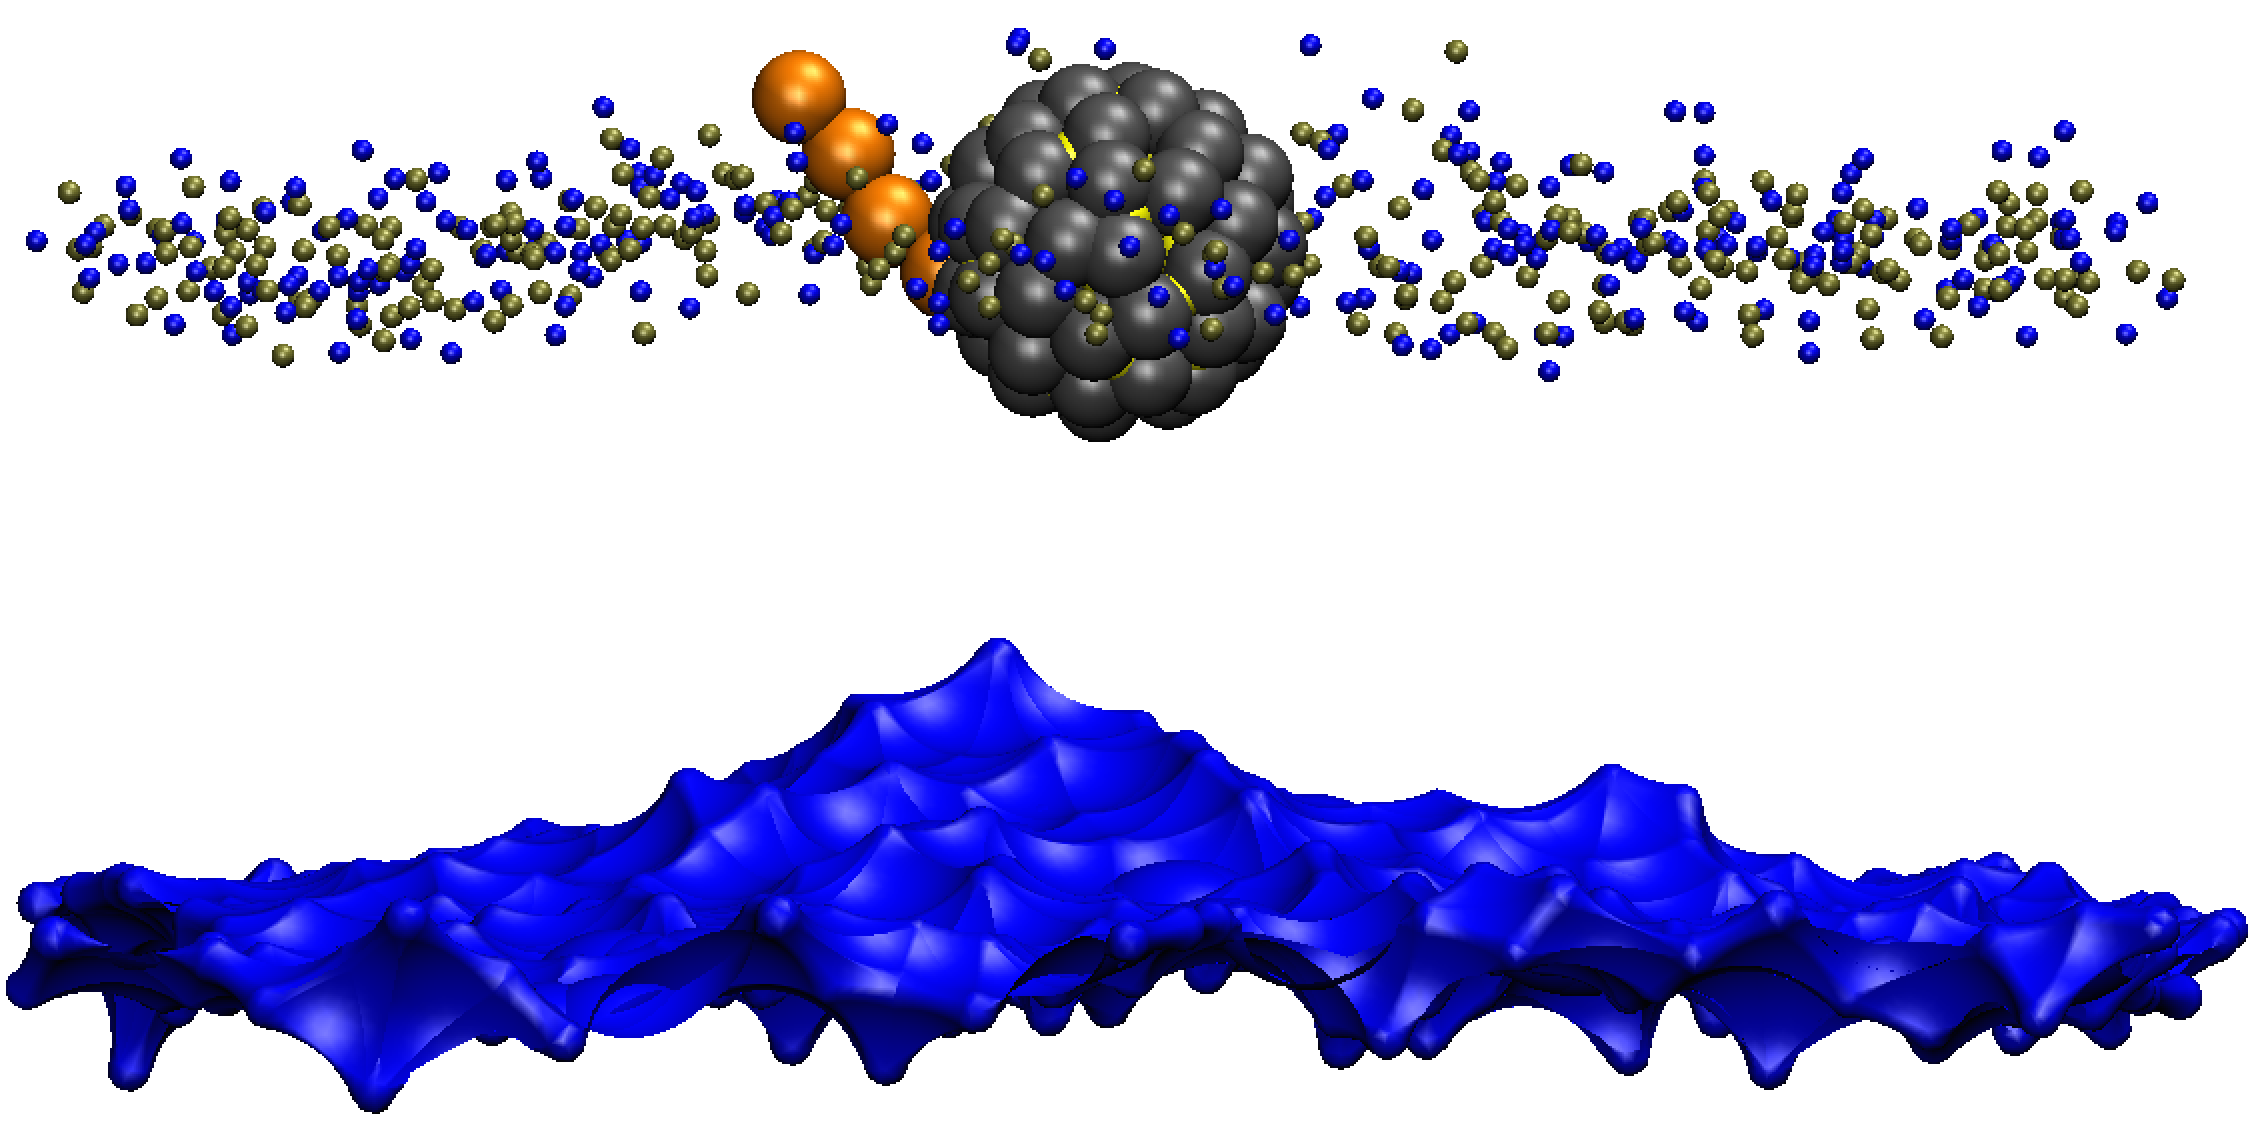
\includegraphics[width=0.47\linewidth]{./img/engulfmentFrame/b.png}%
		}\\\bigskip%
		\subfloat[Atomistic unbiased run]{%
			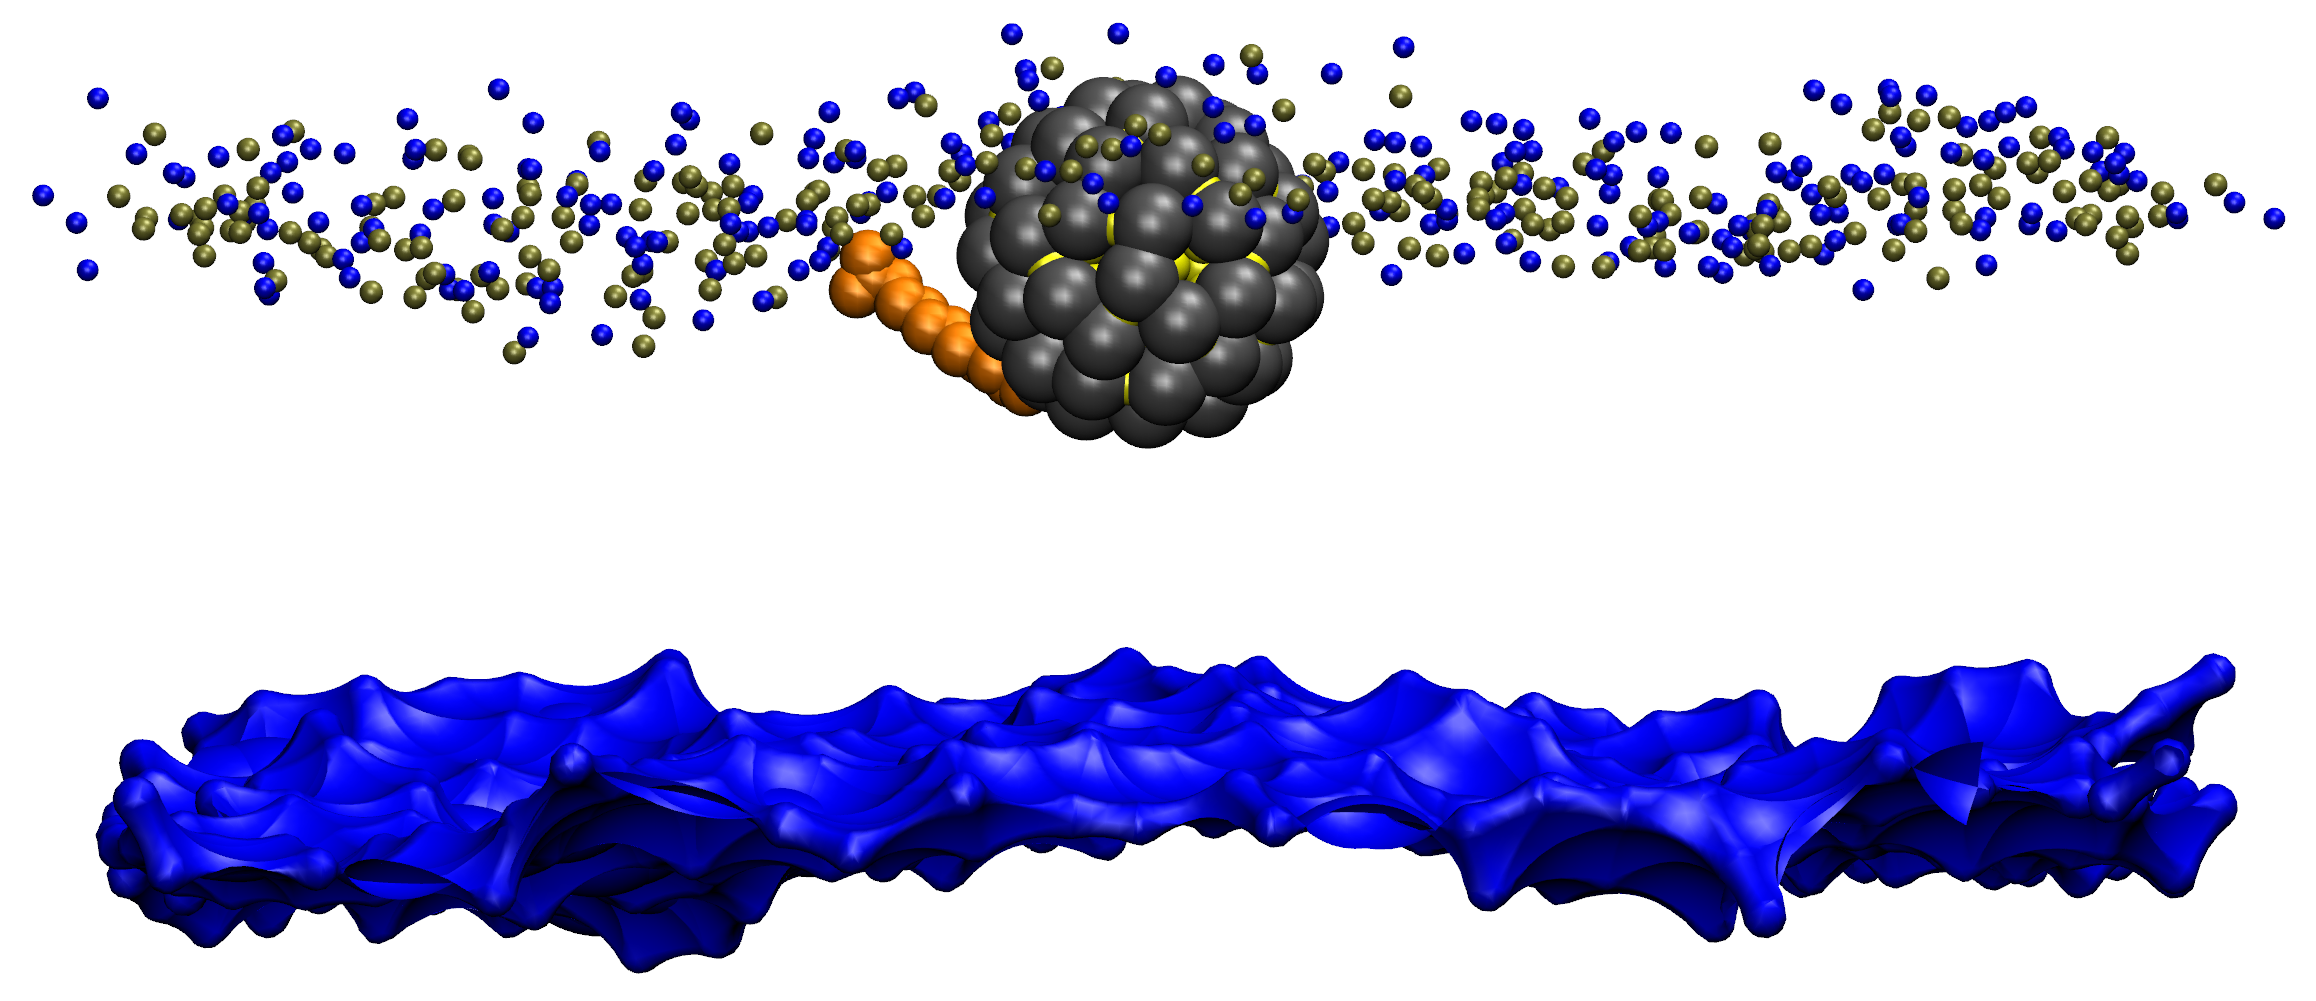
\includegraphics[width=0.47\linewidth]{./img/engulfmentFrame/atomistic_c.png}%
		}\ %
		\subfloat[Atomistic unbiased run]{
			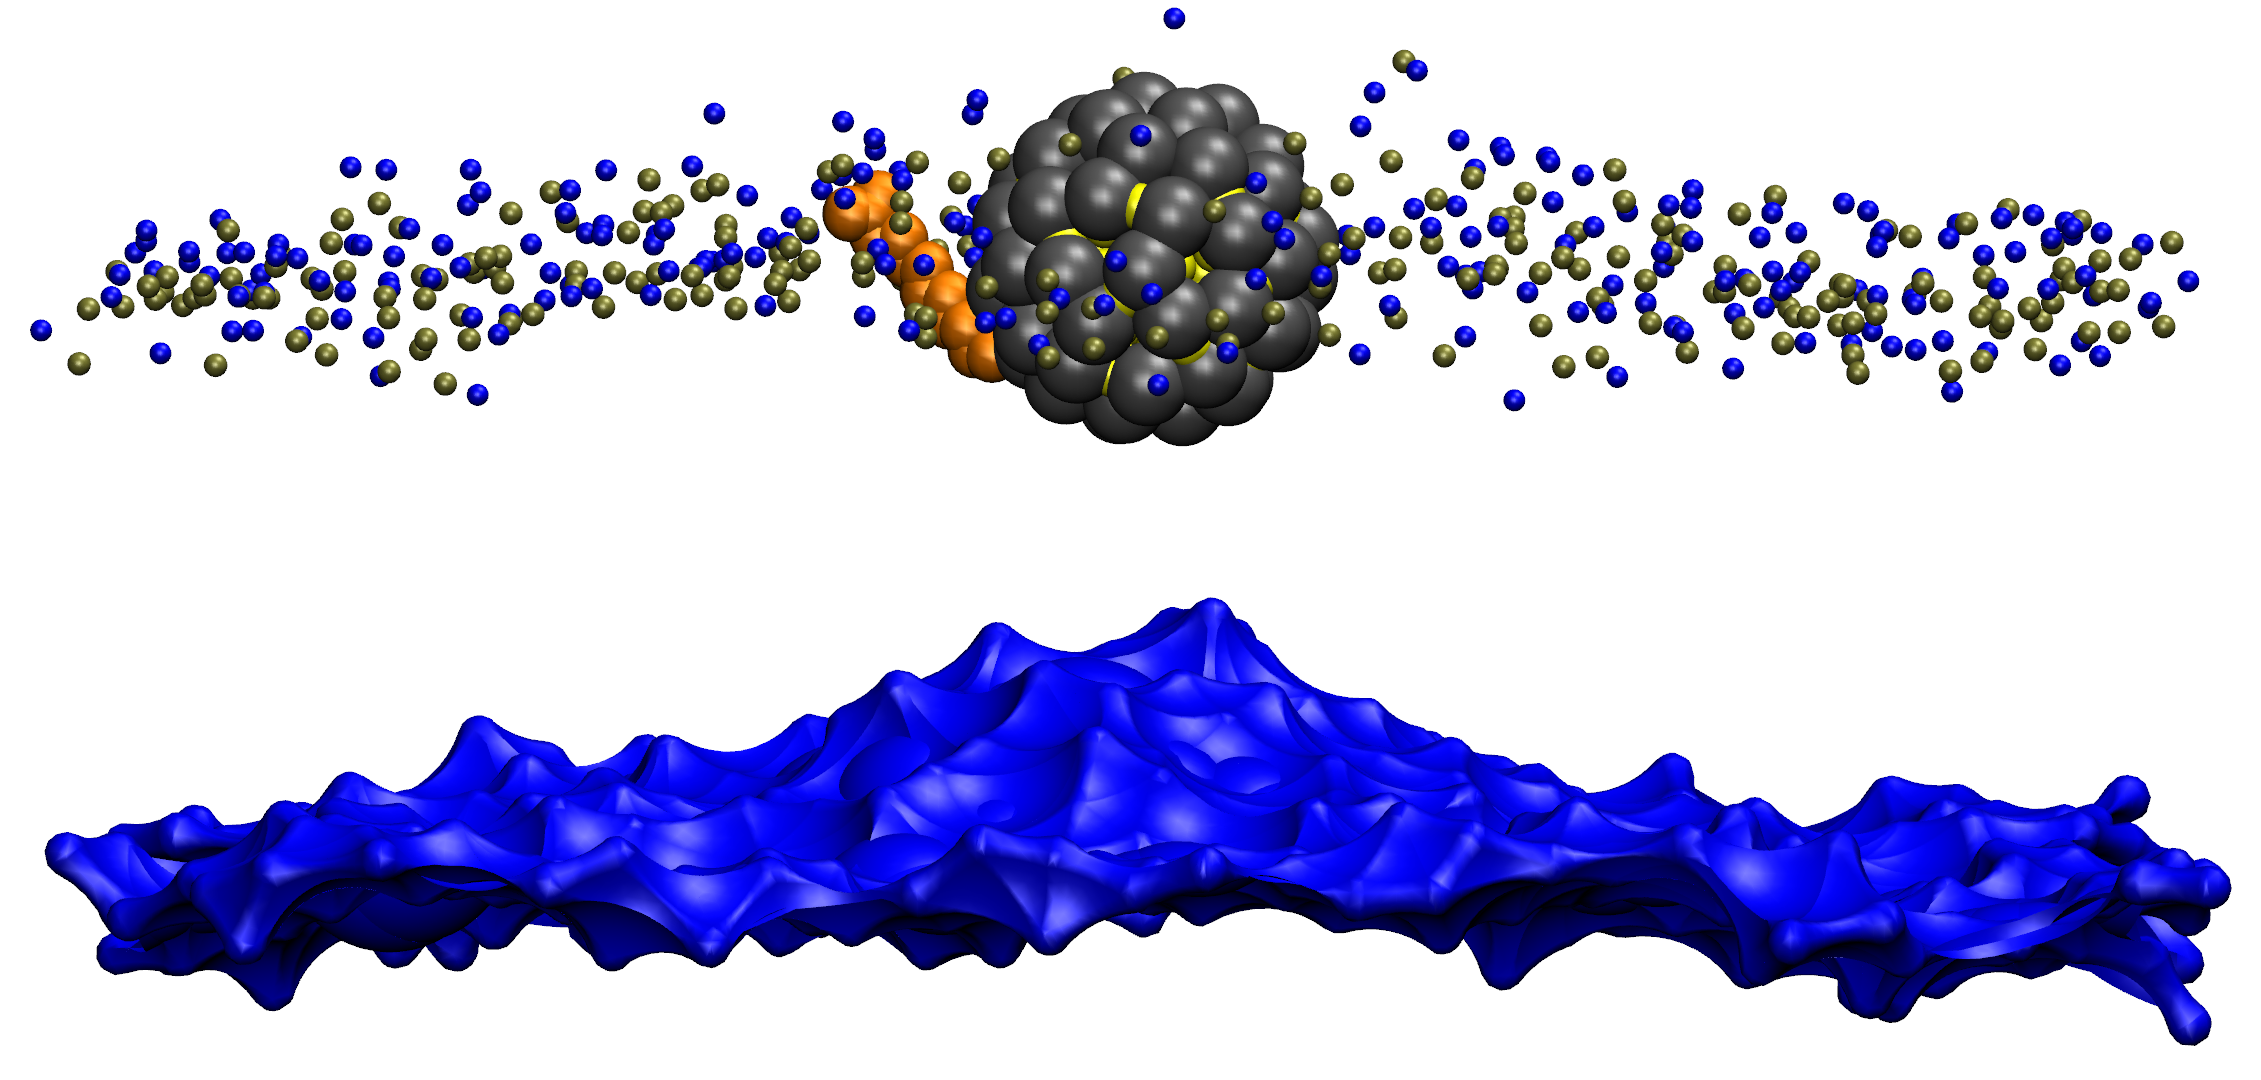
\includegraphics[width=0.47\linewidth]{./img/engulfmentFrame/atomistic_d.png}%
		}\\\bigskip%
		\subfloat[\ac{CG} biased run]{
			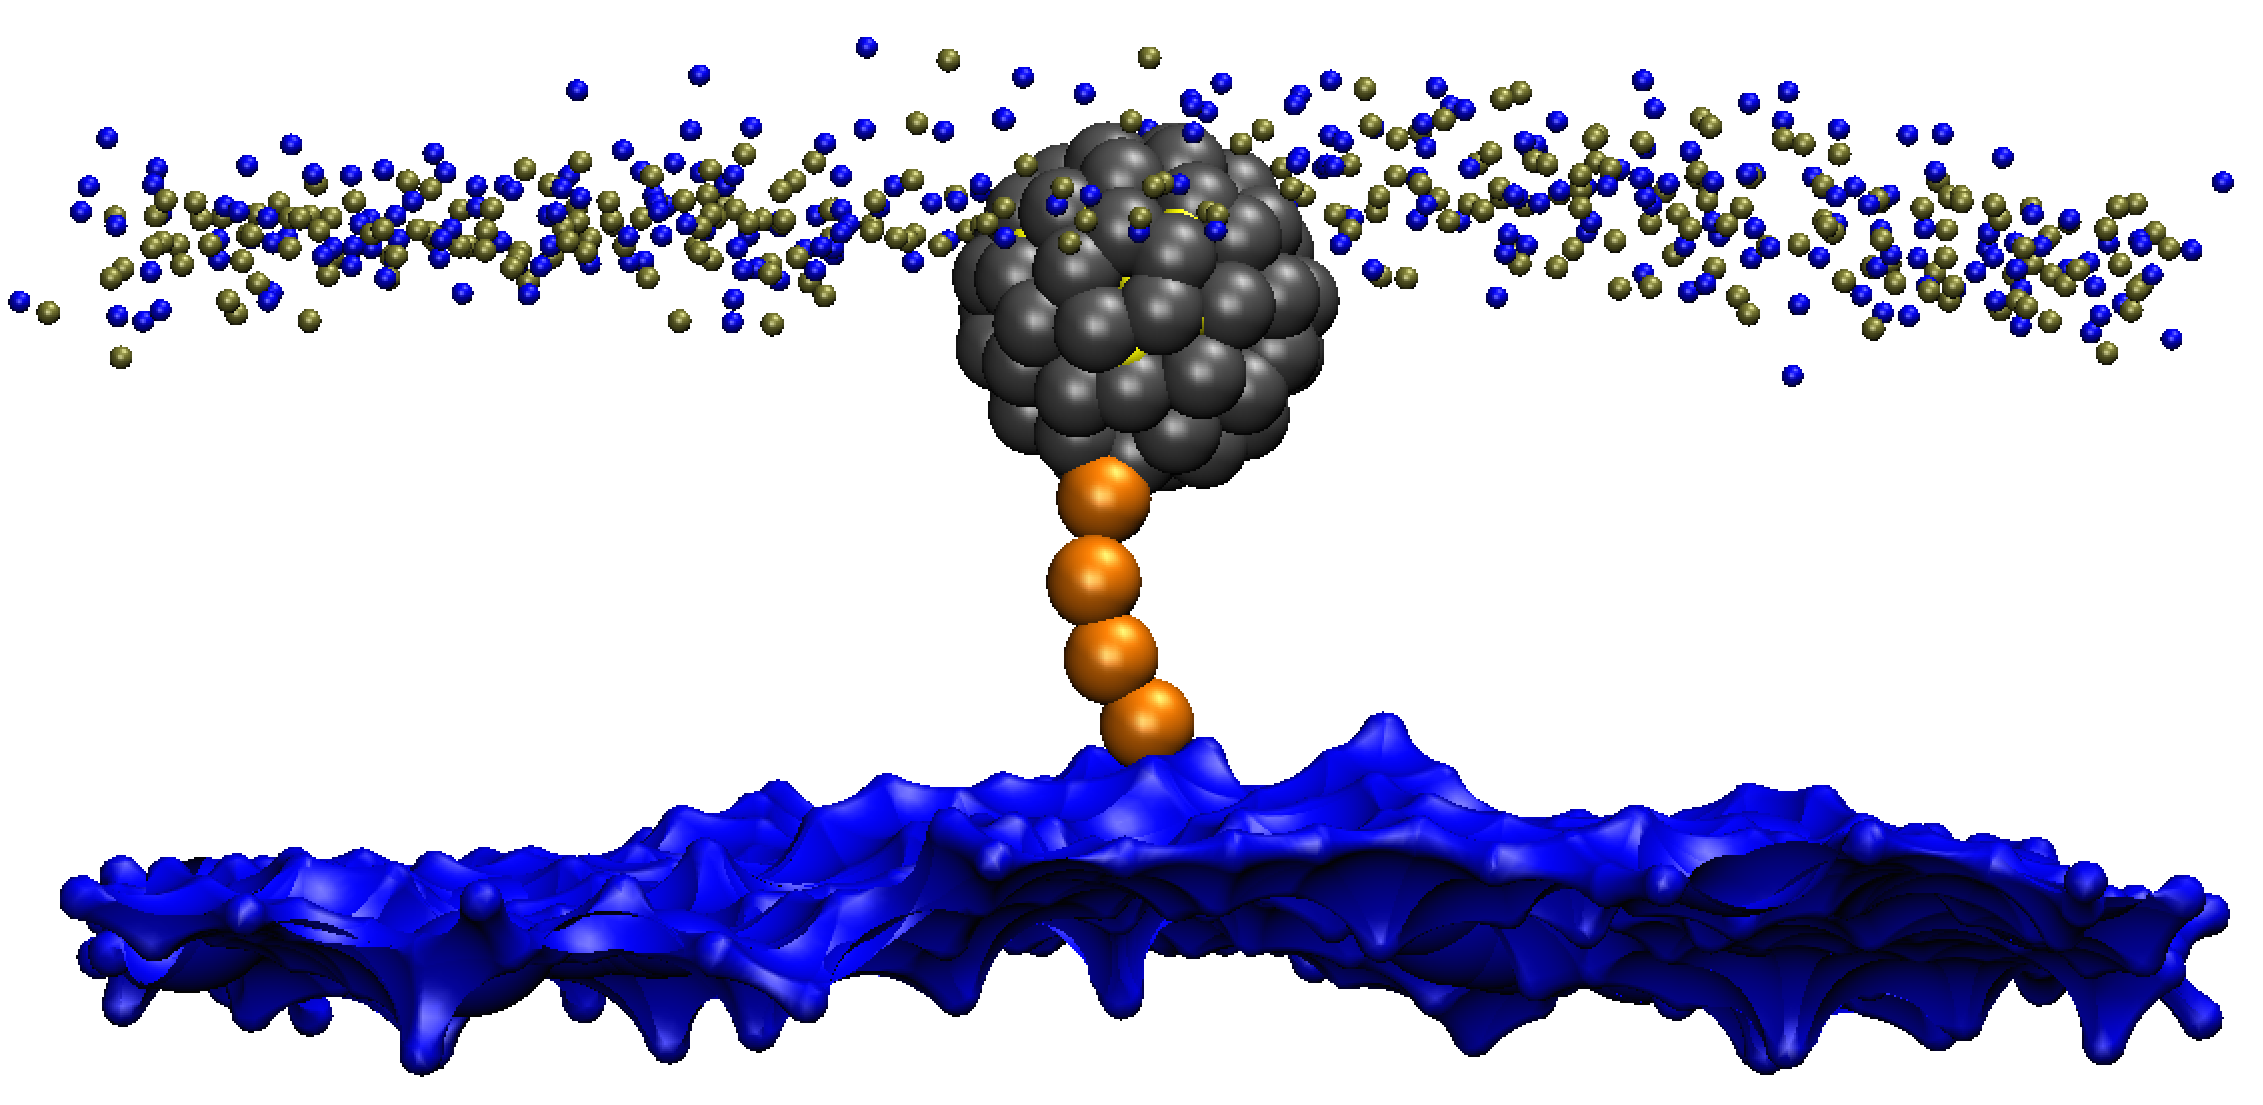
\includegraphics[width=0.47\linewidth]{./img/engulfmentFrame/e.png}%
		}\ %
		\subfloat[\ac{CG} biased run]{
			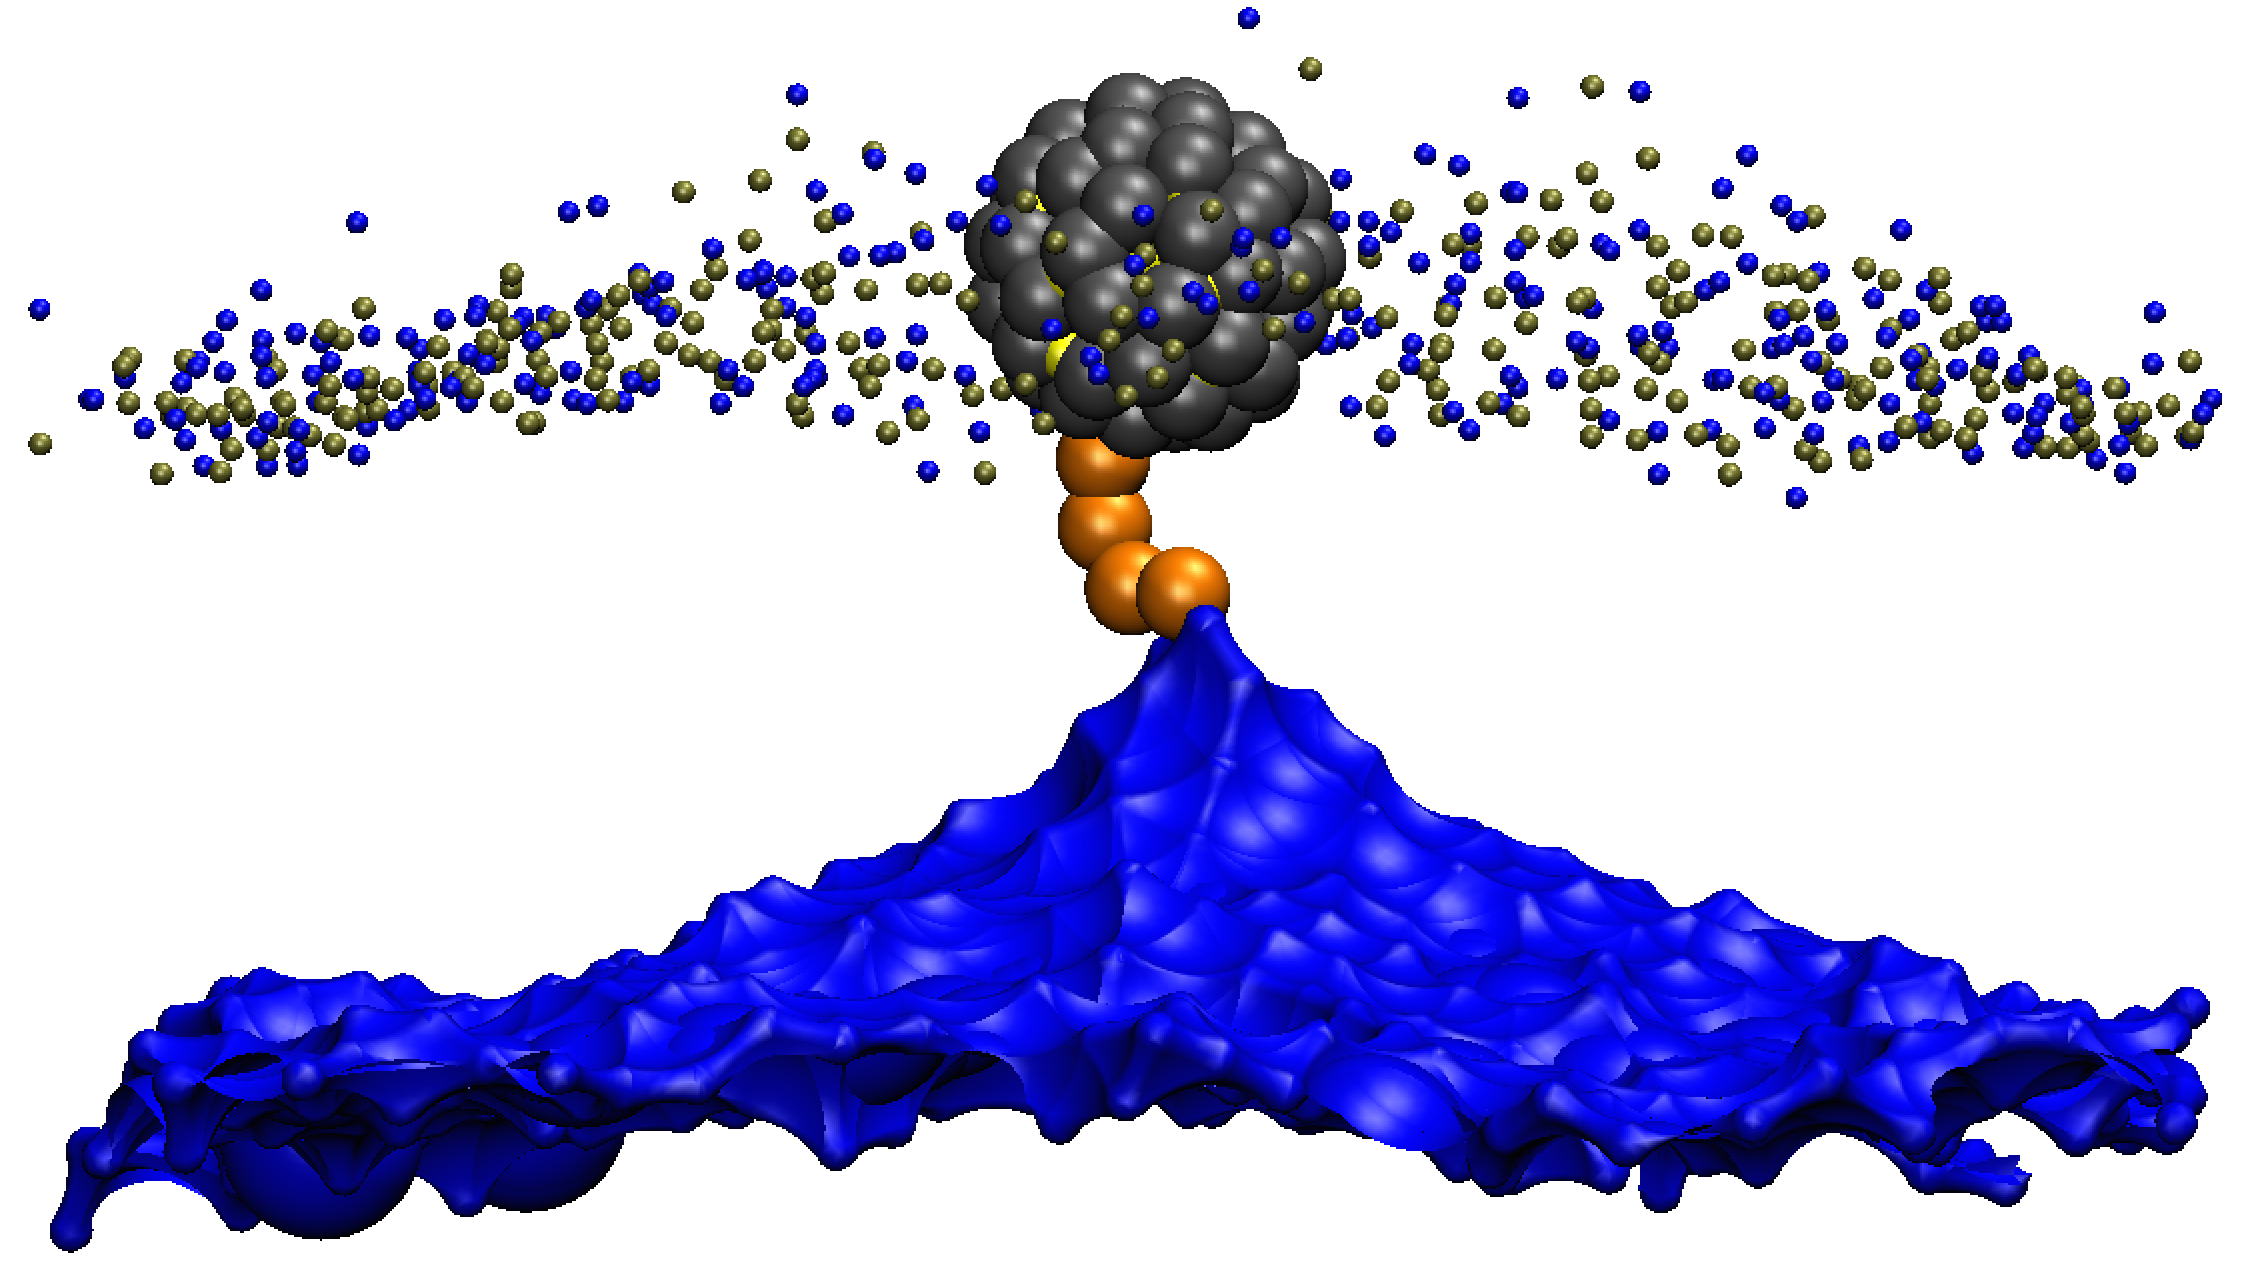
\includegraphics[width=0.47\linewidth]{./img/engulfmentFrame/f.png}%
		}%
		\caption{Snapshots from unbiased and biased simulations showing the deformation of the anchoring leaflet. The top panels refer to my unbiased run of a \acs{CG} striped \acs{NP} with \acs{PME}$+$\acs{PW}, the middle panels refer to an unbiased run of a striped \acs{NP} with atomistic model (figures courtesy of F. Simonelli) and the bottom panels refer to a biased run of a \acs{CG} striped \acs{NP} with \acs{PME}$+$\acs{PW}. In the left panels we see the anchoring leaflet with no appreciable deformation while in the right panels we see the distortion of the anchoring leaflet. Color code as in figure~(\ref{fig:threeProcess}). The surface in blue is the surface representation of the choline and phosphate groups. The charged ligand chosen for the metadynamics is in orange. Water beads, lipid tails and the other \acs{NP} ligands are not shown.}%
		\label{fig:engulfmentFrame}
\end{figure}

\begin{figure}[p]
	\centering
		\subfloat[Entrance leaflet: POPC]{
		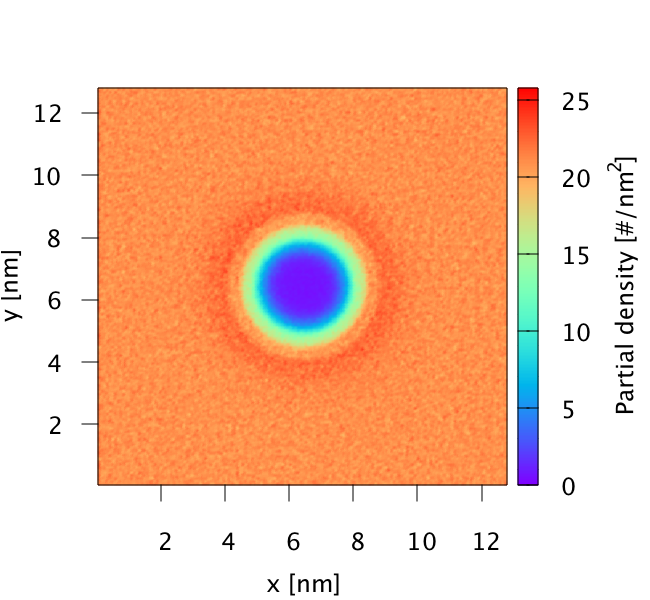
\includegraphics[width=0.5\textwidth]{./img/density_RDF/patched/down.png}
		}%
		\subfloat[Opposite leaflet: POPC]{
		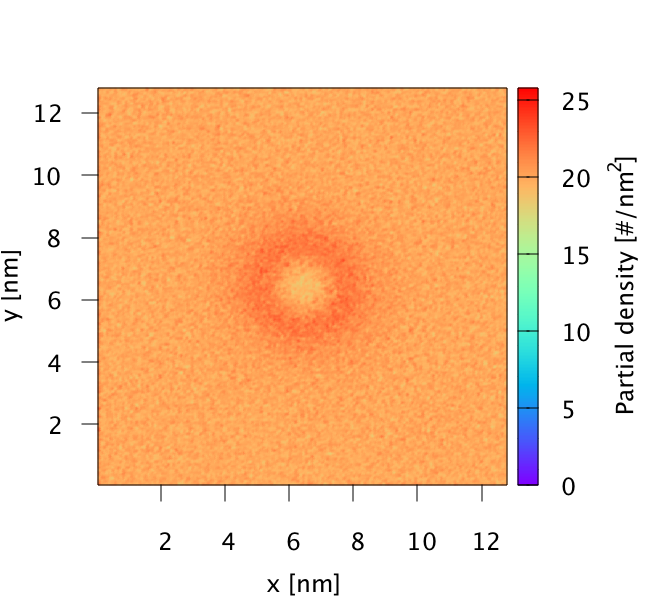
\includegraphics[width=0.5\textwidth]{./img/density_RDF/patched/up.png}
		}\\%
		\subfloat[Entrance leaflet: lipid head]{
		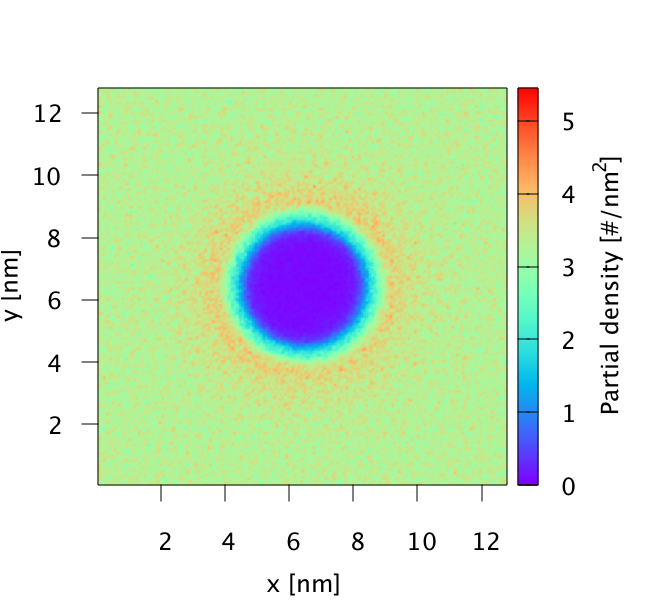
\includegraphics[width=0.5\textwidth]{./img/density_RDF/patched/NC3PO4Down.png}
		}%
		\subfloat[Opposite leaflet: lipid head]{
		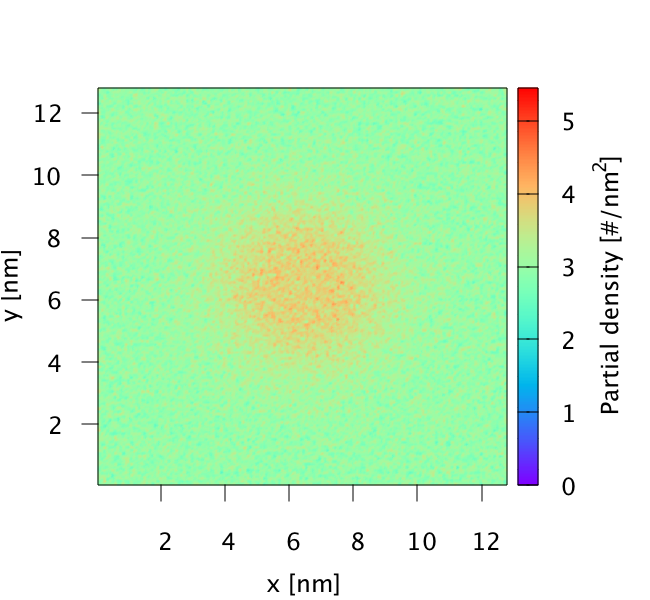
\includegraphics[width=0.5\textwidth]{./img/density_RDF/patched/NC3PO4Up.png}
		}\\%
		\subfloat[Entrance leaflet: lipid tail]{
		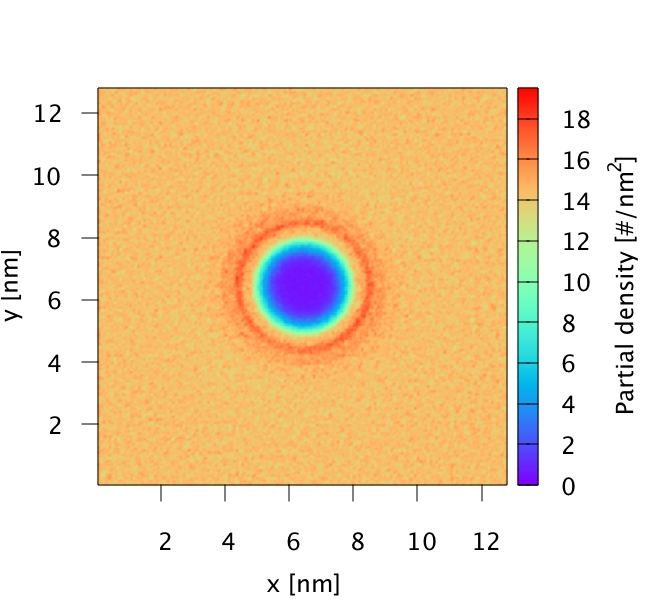
\includegraphics[width=0.5\textwidth]{./img/density_RDF/patched/tailDown.png}
		}%
		\subfloat[Opposite leaflet: lipid tail]{
		\includegraphics[width=0.5\textwidth]{./img/density_RDF/patched/tailUp.png}
		}%
	\caption{Density map for the striped (\acs{MUS}:\acs{OT} $1$:$1$) \acs{NP} in the hydrophobic state of my unbiased run. Left (a), (c) and (e) panels refer to the entrance leaflet. Right (b), (d) and (f) panels refer to the opposite leaflet.}%
	\label{fig:stripedDensity}
\end{figure}

\begin{figure}[p]
	\centering
		\subfloat[Entrance leaflet: POPC]{
		\includegraphics[width=0.5\textwidth]{./img/density_RDF/random/up.png}
		}%
		\subfloat[Opposite leaflet: POPC]{
		\includegraphics[width=0.5\textwidth]{./img/density_RDF/random/down.png}
		}\\%
		\subfloat[Entrance leaflet: lipid head]{
		\includegraphics[width=0.5\textwidth]{./img/density_RDF/random/NC3PO4Up.png}
		}%
		\subfloat[Opposite leaflet: lipid head]{
		\includegraphics[width=0.5\textwidth]{./img/density_RDF/random/NC3PO4Down.png}
		}\\%
		\subfloat[Entrance leaflet: lipid tail]{
		\includegraphics[width=0.5\textwidth]{./img/density_RDF/random/tailUp.png}
		}%
		\subfloat[Opposite leaflet: lipid tail]{
		\includegraphics[width=0.5\textwidth]{./img/density_RDF/random/tailDown.png}
		}
	\caption{Density map for the random (\acs{MUS}:\acs{OT} $1$:$1$) \acs{NP} in the hydrophobic state of my unbiased run. Left (a), (c) and (e) panels refer to the entrance leaflet. Right (b), (d) and (f) panels refer to the opposite leaflet.}%
	\label{fig:randomDensity}
\end{figure}

\begin{figure}[p]
	\centering
		\subfloat[Entrance leaflet: POPC]{
		\includegraphics[width=0.5\textwidth]{./img/density_RDF/random21/up.png}
		}%
		\subfloat[Opposite leaflet: POPC]{
		\includegraphics[width=0.5\textwidth]{./img/density_RDF/random21/down.png}
		}\\%
		\subfloat[Entrance leaflet: lipid head]{
		\includegraphics[width=0.5\textwidth]{./img/density_RDF/random21/NC3PO4Up.png}
		}%
		\subfloat[Opposite leaflet: lipid head]{
		\includegraphics[width=0.5\textwidth]{./img/density_RDF/random21/NC3PO4Down.png}
		}\\%
		\subfloat[Entrance leaflet: lipid tail]{
		\includegraphics[width=0.5\textwidth]{./img/density_RDF/random21/tailUp.png}
		}%
		\subfloat[Opposite leaflet: lipid tail]{
		\includegraphics[width=0.5\textwidth]{./img/density_RDF/random21/tailDown.png}
		}
	\caption{Density map for the random (\acs{MUS}:\acs{OT} $2$:$1$) \acs{NP} in the hydrophobic state of my unbiased run. Left (a), (c) and (e) panels refer to the entrance leaflet. Right (b), (d) and (f) panels refer to the opposite leaflet.}%
	\label{fig:random21Density}
\end{figure}

\begin{figure}[p]
	\centering
		\subfloat[Striped($1$:$1$): Entrance leaflet]{%
		\includegraphics[width=0.5\textwidth]{./img/density_RDF/patched/lipidBottomRDF}
		}%
		\subfloat[Striped($1$:$1$): opposite leaflet]{%
		\includegraphics[width=0.5\textwidth]{./img/density_RDF/patched/lipidTopRDF}
		}\\%
		\subfloat[Random($1$:$1$): entrance leaflet]{%
		\includegraphics[width=0.5\textwidth]{./img/density_RDF/random/lipidTopRDF}
		}%
		\subfloat[Random($1$:$1$): opposite leaflet]{%
		\includegraphics[width=0.5\textwidth]{./img/density_RDF/random/lipidBottomRDF}
		}\\%
		\subfloat[Random($2$:$1$): entrance leaflet]{%
		\includegraphics[width=0.5\textwidth]{./img/density_RDF/random21/lipidTopRDF}
		}%
		\subfloat[Random($2$:$1$): opposite leaflet]{%
		\includegraphics[width=0.5\textwidth]{./img/density_RDF/random21/lipidBottomRDF}
		}%
		\caption{\acs{RDF} centered to the \acs{NP} \acs{COM} of the lipid tails (green) and the lipid heads (violet). The left panels refer to the entrance leaflet, the right to the opposite one. (a) and (b) panels refer to the striped (\acs{MUS}:\acs{OT} $1$:$1$) \acs{NP}. (c) and (d) panels refer to the random (\acs{MUS}:\acs{OT} $1$:$1$) \acs{NP}. (e) and (f) panels refers to the random (\acs{MUS}:\acs{OT} $2$:$1$) \acs{NP}. All \acp{NP} are in the hydrophobic state and refers to my unbiased runs.}%
		\label{fig:RDF}
\end{figure}
